%-------------------------------------------------------------------------------------
%\documentclass[a4paper, 11pt, oneside, openany]{ThesisStyle}
\documentclass[a4paper, 11pt, twoside, openany]{ThesisStyle}

%-------------------------------------------------------------------------------------
\usepackage{amsmath}
\usepackage{amssymb}
\usepackage{latexsym}
\usepackage{graphicx}
\usepackage{epsfig}
\usepackage{epstopdf}
\usepackage{color}
\usepackage{url}
\usepackage{cite}
\usepackage[nottoc]{tocbibind}
\usepackage{multirow}
\usepackage[left=1.2in, right=1in, top=1in, bottom=1in, includefoot, headheight=13.6pt]{geometry}
\usepackage{array} %allow commands for the table columns specification
\usepackage{subfigure} %for column figures
\usepackage{floatflt} %for floating (wrapped) figures
\usepackage[british]{babel} % For british english hyphenation patterns
\usepackage[font=small, labelfont=bf]{caption} % Captions
\usepackage{url} % Formatting for URL's i.e. http://www.rhizobia.co.nz
\usepackage{microtype} % makes pdf look better
\usepackage[nottoc]{tocbibind} % Table of contents
\usepackage[hyperindex=true,pdftitle={Search for diboson resonances with CMS and Pixel Barrel Detector  Calibration and Upgrade},pdfauthor={Jennifer Ngadiuba},colorlinks=false,pagebackref=false,citecolor=blue,plainpages=false,filecolor=blue,linkcolor=blue,urlcolor=blue,pdfpagelabels]{hyperref} % colourlinks=false for printing 
\usepackage{xspace}
\usepackage{fancyhdr}
%\usepackage[colorlinks=true,citecolor=blue,filecolor=blue,linkcolor=blue,urlcolor=blue,pdftex]{hyperref}
%\usepackage{capt-of} % needed to put table next to a figure and have captions
%\usepackage{natbib} % The best package for bibliographies
%\usepackage[width=11cm,font=footnotesize,labelfont=bf, format=default,justification=centerlast]{caption} % Captions\usepackage{fancyhdr} % Change caption style; changes headers and page styles etc.
%\usepackage{natbib}

%-------------------------------------------------------------------------------------
\pagestyle{fancy}
% with this we ensure that the chapter and section
% headings are in lowercase.
\renewcommand{\chaptermark}[1]{\markboth{#1}{}}
\renewcommand{\sectionmark}[1]{\markright{\thesection\ #1}}
\fancyhf{} % delete current setting for header and footer
\fancyhead[LE,RO]{\bfseries\thepage}
\fancyhead[LO]{\bfseries\rightmark}
\fancyhead[RE]{\bfseries\leftmark}
%\renewcommand{\headrulewidth}{0.5pt}
%\renewcommand{\footrulewidth}{0pt}
\addtolength{\headheight}{0.5pt} % make space for the rule
%\fancypagestyle{plain}{%
%\fancyhead{} % get rid of headers on plain pages
%\renewcommand{\headrulewidth}{0pt} % and the line
%-------------------------------------------------------------------------------------

%-------------------------------------------------------------------------------------
\providecommand{\FIXME}[1]{\textcolor{red}{{\sffamily{\bfseries{}FIXME:} #1}}}
\newcommand{\chone}{chapters/Chapter1-Introduction/Figures}
\newcommand{\chtwo}{chapters/Chapter2-Theory/Figures}
\newcommand{\chthree}{chapters/Chapter3-CMSatLHC/Figures}
\newcommand{\chfour}{chapters/Chapter4-DibosonIntro/Figures}
\newcommand{\chfive}{chapters/Chapter5-DataAndSimulation/Figures}
\newcommand{\chsix}{chapters/Chapter6-Objects/Figures}
\newcommand{\chseven}{chapters/Chapter7-JetSubstructure/Figures}
\newcommand{\cheight}{chapters/Chapter8-AnalysisStrategy/Figures}
\newcommand{\chnine}{chapters/Chapter9-Results8TeV/Figures}
\newcommand{\chten}{chapters/Chapter10-Results13TeV/Figures}
\newcommand{\cheleven}{chapters/Chapter11-Combination/Figures}
\newcommand{\mWH}{\ensuremath{m_{\rm WH}}\xspace}
\newcommand{\mWV}{\ensuremath{m_{\rm WV}}\xspace}
\newcommand{\mlvj}{\ensuremath{m_{\ell\nu+{\rm jet}}}\xspace}
\newcommand{\mJ}{\ensuremath{m_{\text{jet}}}\xspace} 
\newcommand{\nsubj}{\ensuremath{\tau_{21}}\xspace}%
\newcommand{\lnujet}{\ensuremath{\ell \nu}+jet\xspace}
\newcommand{\lnuHjet}{\ensuremath{\ell \nu}+\bbbar\xspace}
\newcommand{\WMASSDATAWPT} {\ensuremath{84.6\pm0.7}\xspace}
\newcommand{\WRESDATAWPT} {\ensuremath{8.2\pm0.7}\xspace}
\newcommand{\WMASSMCWPT} {\ensuremath{85.1\pm0.2}\xspace}
\newcommand{\WRESMCWPT} {\ensuremath{7.8\pm0.3}\xspace}

%-------------------------------------------------------------------------------------
%%%%%%%%%%%%%%%%%%%%%%%%%%%%%%%%%%%%%%%%%%%%%%%%%%%%%%%%%%%%%%%%%%%%
%
%  Common definitions
%
%  N.B. use of \providecommand rather than \newcommand means
%       that a definition is ignored if already specified
%
%                                              L. Taylor 18 Feb 2005
%%%%%%%%%%%%%%%%%%%%%%%%%%%%%%%%%%%%%%%%%%%%%%%%%%%%%%%%%%%%%%%%%%%%

% Some shorthand
% turn off italics
\newcommand {\etal}{\mbox{et al.}\xspace} %et al. - no preceding comma
\newcommand {\ie}{\mbox{i.e.}\xspace}     %i.e.
\newcommand {\eg}{\mbox{e.g.}\xspace}     %e.g.
\newcommand {\etc}{\mbox{etc.}\xspace}     %etc.
\newcommand {\vs}{\mbox{\sl vs.}\xspace}      %vs.
\newcommand {\mdash}{\ensuremath{\mathrm{-}}} % for use within formulas

% some terms whose definition we may change
\newcommand {\Lone}{Level-1\xspace} % Level-1 or L1 ?
\newcommand {\Ltwo}{Level-2\xspace}
\newcommand {\Lthree}{Level-3\xspace}

% Some software programs (alphabetized)
\providecommand{\ACERMC} {\textsc{AcerMC}\xspace}
\newcommand{\amcatnlo}{\textsc{madgraph5\_amc@nlo}\xspace}
\providecommand{\ALPGEN} {{\textsc{alpgen}}\xspace}
\providecommand{\CHARYBDIS} {{\textsc{charybdis}}\xspace}
\providecommand{\CMKIN} {\textsc{cmkin}\xspace}
\providecommand{\CMSIM} {{\textsc{cmsim}}\xspace}
\providecommand{\CMSSW} {{\textsc{cmssw}}\xspace}
\providecommand{\COBRA} {{\textsc{cobra}}\xspace}
\providecommand{\COCOA} {{\textsc{cocoa}}\xspace}
\providecommand{\COMPHEP} {\textsc{CompHEP}\xspace}
\providecommand{\EVTGEN} {{\textsc{evtgen}}\xspace}
\providecommand{\FAMOS} {{\textsc{famos}}\xspace}
\providecommand{\GARCON} {\textsc{garcon}\xspace}
\providecommand{\GARFIELD} {{\textsc{garfield}}\xspace}
\providecommand{\GEANE} {{\textsc{geane}}\xspace}
\providecommand{\GEANTfour} {{\textsc{geant4}}\xspace}
\providecommand{\GEANTthree} {{\textsc{geant3}}\xspace}
\providecommand{\GEANT} {{\textsc{geant}}\xspace}
\providecommand{\HDECAY} {\textsc{hdecay}\xspace}
\providecommand{\HERWIG} {{\textsc{herwig}}\xspace}
\providecommand{\HIGLU} {{\textsc{higlu}}\xspace}
\providecommand{\HIJING} {{\textsc{hijing}}\xspace}
\providecommand{\IGUANA} {\textsc{iguana}\xspace}
\providecommand{\ISAJET} {{\textsc{isajet}}\xspace}
\providecommand{\ISAPYTHIA} {{\textsc{isapythia}}\xspace}
\providecommand{\ISASUGRA} {{\textsc{isasugra}}\xspace}
\providecommand{\ISASUSY} {{\textsc{isasusy}}\xspace}
\providecommand{\ISAWIG} {{\textsc{isawig}}\xspace}
\providecommand{\MADGRAPH} {\textsc{MadGraph}\xspace}
\providecommand{\MCATNLO} {\textsc{mc@nlo}\xspace}
\providecommand{\MCFM} {\textsc{mcfm}\xspace}
\providecommand{\MILLEPEDE} {{\textsc{millepede}}\xspace}
\providecommand{\ORCA} {{\textsc{orca}}\xspace}
\providecommand{\OSCAR} {{\textsc{oscar}}\xspace}
\providecommand{\PHOTOS} {\textsc{photos}\xspace}
\providecommand{\POWHEG} {{\textsc{powheg}}\xspace}
\providecommand{\PROSPINO} {\textsc{prospino}\xspace}
\providecommand{\PYTHIA} {{\textsc{pythia}}\xspace}
\providecommand{\SHERPA} {{\textsc{sherpa}}\xspace}
\providecommand{\TAUOLA} {\textsc{tauola}\xspace}
\providecommand{\TOPREX} {\textsc{TopReX}\xspace}
\providecommand{\XDAQ} {{\textsc{xdaq}}\xspace}

%  Experiments
\newcommand {\DZERO}{D\O\xspace}     %etc.


% Measurements and units...

\newcommand{\de}{\ensuremath{^\circ}}
\newcommand{\ten}[1]{\ensuremath{\times \text{10}^\text{#1}}}
\newcommand{\unit}[1]{\ensuremath{\text{\,#1}}\xspace}
\newcommand{\mum}{\ensuremath{\,\mu\text{m}}\xspace}
\newcommand{\micron}{\ensuremath{\,\mu\text{m}}\xspace}
\newcommand{\cm}{\ensuremath{\,\text{cm}}\xspace}
\newcommand{\mm}{\ensuremath{\,\text{mm}}\xspace}
\newcommand{\mus}{\ensuremath{\,\mu\text{s}}\xspace}
\newcommand{\keV}{\ensuremath{\,\text{ke\hspace{-.08em}V}}\xspace}
\newcommand{\MeV}{\ensuremath{\,\text{Me\hspace{-.08em}V}}\xspace}
\newcommand{\GeV}{\ensuremath{\,\text{Ge\hspace{-.08em}V}}\xspace}
\newcommand{\TeV}{\ensuremath{\,\text{Te\hspace{-.08em}V}}\xspace}
\newcommand{\PeV}{\ensuremath{\,\text{Pe\hspace{-.08em}V}}\xspace}
\newcommand{\keVc}{\ensuremath{{\,\text{ke\hspace{-.08em}V\hspace{-0.16em}/\hspace{-0.08em}}c}}\xspace}
\newcommand{\MeVc}{\ensuremath{{\,\text{Me\hspace{-.08em}V\hspace{-0.16em}/\hspace{-0.08em}}c}}\xspace}
\newcommand{\GeVc}{\ensuremath{{\,\text{Ge\hspace{-.08em}V\hspace{-0.16em}/\hspace{-0.08em}}c}}\xspace}
\newcommand{\TeVc}{\ensuremath{{\,\text{Te\hspace{-.08em}V\hspace{-0.16em}/\hspace{-0.08em}}c}}\xspace}
\newcommand{\keVcc}{\ensuremath{{\,\text{ke\hspace{-.08em}V\hspace{-0.16em}/\hspace{-0.08em}}c^\text{2}}}\xspace}
\newcommand{\MeVcc}{\ensuremath{{\,\text{Me\hspace{-.08em}V\hspace{-0.16em}/\hspace{-0.08em}}c^\text{2}}}\xspace}
\newcommand{\GeVcc}{\ensuremath{{\,\text{Ge\hspace{-.08em}V\hspace{-0.16em}/\hspace{-0.08em}}c^\text{2}}}\xspace}
\newcommand{\TeVcc}{\ensuremath{{\,\text{Te\hspace{-.08em}V\hspace{-0.16em}/\hspace{-0.08em}}c^\text{2}}}\xspace}

\newcommand{\pbinv} {\mbox{\ensuremath{\,\text{pb}^\text{$-$1}}}\xspace}
\newcommand{\fbinv} {\mbox{\ensuremath{\,\text{fb}^\text{$-$1}}}\xspace}
\newcommand{\nbinv} {\mbox{\ensuremath{\,\text{nb}^\text{$-$1}}}\xspace}
\newcommand{\percms}{\ensuremath{\,\text{cm}^\text{$-$2}\,\text{s}^\text{$-$1}}\xspace}
\newcommand{\lumi}{\ensuremath{\mathcal{L}}\xspace}
\newcommand{\Lumi}{\ensuremath{\mathcal{L}}\xspace}%both upper and lower
%
% Need a convention here:
\newcommand{\LvLow}  {\ensuremath{\mathcal{L}=\text{10}^\text{32}\,\text{cm}^\text{$-$2}\,\text{s}^\text{$-$1}}\xspace}
\newcommand{\LLow}   {\ensuremath{\mathcal{L}=\text{10}^\text{33}\,\text{cm}^\text{$-$2}\,\text{s}^\text{$-$1}}\xspace}
\newcommand{\lowlumi}{\ensuremath{\mathcal{L}=\text{2}\times \text{10}^\text{33}\,\text{cm}^\text{$-$2}\,\text{s}^\text{$-$1}}\xspace}
\newcommand{\LMed}   {\ensuremath{\mathcal{L}=\text{2}\times \text{10}^\text{33}\,\text{cm}^\text{$-$2}\,\text{s}^\text{$-$1}}\xspace}
\newcommand{\LHigh}  {\ensuremath{\mathcal{L}=\text{10}^\text{34}\,\text{cm}^\text{$-$2}\,\text{s}^\text{$-$1}}\xspace}
\newcommand{\hilumi} {\ensuremath{\mathcal{L}=\text{10}^\text{34}\,\text{cm}^\text{$-$2}\,\text{s}^\text{$-$1}}\xspace}

% Some usual physics terms


% SM (still to be classified)

\newcommand{\kt}{\ensuremath{k_{\mathrm{T}}}\xspace}
\newcommand{\BC}{\ensuremath{{B_{\mathrm{c}}}}\xspace}
\newcommand{\bbarc}{\ensuremath{{\overline{b}c}}\xspace}
\newcommand{\bbbar}{\ensuremath{{\mathrm{b}\overline{\mathrm{b}}}}\xspace}
\newcommand{\ccbar}{\ensuremath{{c\overline{c}}}\xspace}
\newcommand{\cPq}{\ensuremath{\mathrm{q}}}
\newcommand{\cPaq}{\ensuremath{\overline{\mathrm{q}}}}
\newcommand{\qqbarpr}{\ensuremath{\cPq\cPaq^({}'^){}}\xspace}
\newcommand{\qqbar}{\ensuremath{\cPq\cPaq}\xspace}
%\newcommand{\ell}{\textit{l}\xspace}
\newcommand{\Pgn}{\ensuremath{\nu}}
\newcommand{\JPsi}{\ensuremath{{J}\hspace{-.08em}/\hspace{-.14em}\psi}\xspace}
\newcommand{\bspsiphi}{\ensuremath{B_s \to \JPsi\, \phi}\xspace}
%\newcommand{\ttbar}{\ensuremath{{t\overline{t}}}\xspace}
\newcommand{\AFB}{\ensuremath{A_\text{FB}}\xspace}
\newcommand{\EE}{\ensuremath{e^+e^-}\xspace}
\newcommand{\MM}{\ensuremath{\mu^+\mu^-}\xspace}
\newcommand{\TT}{\ensuremath{\tau^+\tau^-}\xspace}
\newcommand{\wangle}{\ensuremath{\sin^{2}\theta_{\text{eff}}^\text{lept}(M^2_\mathrm{Z})}\xspace}
%\newcommand{\ttbar}{\ensuremath{{t\overline{t}}}\xspace}
\newcommand{\stat}{\ensuremath{\,\text{(stat.)}}\xspace}
\newcommand{\syst}{\ensuremath{\,\text{(syst.)}}\xspace}
% these moved to similar defs
\newcommand{\Etmiss}{\ensuremath{E_{\mathrm{T}\!{\rm miss}}}}
%\newcommand{\VEtmiss}{\ensuremath{{\vec E}_{\mathrm{T}\!{\rm miss}}}}
\newcommand{\ptvecmiss}{\ensuremath{{\vec p}_{\mathrm{T}}^{\kern1pt\text{miss}}}\xspace}

%%%  E-gamma definitions
\newcommand{\HGG}{\ensuremath{\mathrm{H}\to\gamma\gamma}}
\newcommand{\gev}{\GeV}
\newcommand{\GAMJET}{\ensuremath{\gamma + \text{jet}}}
\newcommand{\PPTOJETS}{\ensuremath{\mathrm{pp}\to\text{jets}}}
\newcommand{\PPTOGG}{\ensuremath{\mathrm{pp}\to\gamma\gamma}}
\newcommand{\PPTOGAMJET}{\ensuremath{\mathrm{pp}\to\gamma +
\mathrm{jet}
}}
\newcommand{\MH}{\ensuremath{\mathrm{M_{\mathrm{H}}}}}
\newcommand{\RNINE}{\ensuremath{\mathrm{R}_\mathrm{9}}}
\newcommand{\DR}{\ensuremath{\Delta\mathrm{R}}}



% Physics symbols ...

\newcommand{\PT}{\ensuremath{p_{\mathrm{T}}}\xspace}
\newcommand{\pt}{\ensuremath{p_{\mathrm{T}}}\xspace}
\newcommand{\ET}{\ensuremath{E_{\mathrm{T}}}\xspace}
\newcommand{\HT}{\ensuremath{H_{\mathrm{T}}}\xspace}
\newcommand{\et}{\ensuremath{E_{\mathrm{T}}}\xspace}
\providecommand{\Em}{\ensuremath{E\hspace{-0.6em}/}\xspace}
\providecommand{\Pm}{\ensuremath{p\hspace{-0.5em}/}\xspace}
\providecommand{\PTm}{\ensuremath{{p}_\mathrm{T}\hspace{-1.02em}/}\xspace}
\providecommand{\PTslash}{\ensuremath{{p}_\mathrm{T}\hspace{-1.02em}/}\xspace}
\newcommand{\ETm}{\ensuremath{E_{\mathrm{T}}^{\text{miss}}}\xspace}
\providecommand{\ETslash}{\ensuremath{E_{\mathrm{T}}\hspace{-1.1em}/}\xspace}
\newcommand{\MET}{\ensuremath{E_{\mathrm{T}}^{\text{miss}}}\xspace}
\newcommand{\ETmiss}{\ensuremath{E_{\mathrm{T}}^{\text{miss}}}\xspace}
\newcommand{\VEtmiss}{\ensuremath{{\vec E}_{\mathrm{T}}^{\;\text{miss}}}\xspace}
\newcommand{\Vpt}{\ensuremath{{\vec p}_{\mathrm{T}}}\xspace}

% roman face derivative
\providecommand{\dd}[2]{\ensuremath{\frac{\mathrm{d} #1}{\mathrm{d} #2}}}
% Particle names which will track the italic/non-italic face convention
%\providecommand{\zp}{\ensuremath{\mathrm{Z}^\prime}\xspace}
\providecommand{\Zpr}{\ensuremath{\mathrm{Z}^\prime}\xspace}
\providecommand{\Wpr}{\ensuremath{\mathrm{W}^\prime}\xspace}
\providecommand{\BulkG}{\ensuremath{\mathrm{G}_\mathrm{bulk}}\xspace}

\providecommand{\JPsi}{\ensuremath{\mathrm{J}\hspace{-.08em}/\hspace{-.14em}\psi}\xspace}
\providecommand{\Z}{\ensuremath{\mathrm{Z}}\xspace}
\providecommand{\ttbar}{\ensuremath{\mathrm{t}\overline{\mathrm{t}}}\xspace}
% Extensions for missing names in PENNAMES
\providecommand{\cPgn}{\ensuremath{\nu}\xspace} % generic neutrino
\providecommand{\cPJgy}{\JPsi} % J/Psi (no mass)
\providecommand{\cPZ}{\Z} % plain Z (no superscript 0)
\providecommand{\cPZpr}{\Zpr} % plain Z'
\providecommand{\cPWpr}{\Wpr} % plain W'
\providecommand{\PWpr}{\ensuremath{\mathrm{W}^\prime}\xspace} % use prime like pennames2
\providecommand{\PZpr}{\ensuremath{\mathrm{Z}^\prime}\xspace} % plain Z' using prime
\providecommand{\PVpr}{\ensuremath{\mathrm{V}^\prime}\xspace} % plain Z' using prime
% SymbolFace not yet available in trunk version
%\providecommand{\cPqb}{\ensuremath{\cmsSymbolFace{b}}\xspace} % b for b quark
%\providecommand{\cPqt}{\ensuremath{\cmsSymbolFace{t}}\xspace} % t for t quark
%\providecommand{\cPqc}{\ensuremath{\cmsSymbolFace{c}}\xspace} % c for c quark
%\providecommand{\cPaqb}{\ensuremath{\overline{\cmsSymbolFace{b}}\xspace}} % b for b anti-quark
%\providecommand{\cPaqt}{\ensuremath{\overline{\cmsSymbolFace{t}}}\xspace} % t for t anti-quark
%\providecommand{\cPaqc}{\ensuremath{\overline{\cmsSymbolFace{c}}}\xspace} % c for c anti-quark
%%%%%%
% From Albert
%

\newcommand{\ga}{\ensuremath{\gtrsim}}
\newcommand{\la}{\ensuremath{\lesssim}}
%\def\ga{\mathrel{\rlap{\raise.6ex\hbox{$>$}}{\lower.6ex\hbox{$\sim$}}}}
%\def\la{\mathrel{\rlap{\raise.6ex\hbox{$<$}}{\lower.6ex\hbox{$\sim$}}}}
%
\newcommand{\swsq}{\ensuremath{\sin^2\theta_W}\xspace}
\newcommand{\cwsq}{\ensuremath{\cos^2\theta_W}\xspace}
\newcommand{\tanb}{\ensuremath{\tan\beta}\xspace}
\newcommand{\tanbsq}{\ensuremath{\tan^{2}\beta}\xspace}
\newcommand{\sidb}{\ensuremath{\sin 2\beta}\xspace}
\newcommand{\alpS}{\ensuremath{\alpha_S}\xspace}
\newcommand{\alpt}{\ensuremath{\tilde{\alpha}}\xspace}

\newcommand{\QL}{\ensuremath{Q_L}\xspace}
\newcommand{\sQ}{\ensuremath{\tilde{Q}}\xspace}
\newcommand{\sQL}{\ensuremath{\tilde{Q}_L}\xspace}
\newcommand{\ULC}{\ensuremath{U_L^C}\xspace}
\newcommand{\sUC}{\ensuremath{\tilde{U}^C}\xspace}
\newcommand{\sULC}{\ensuremath{\tilde{U}_L^C}\xspace}
\newcommand{\DLC}{\ensuremath{D_L^C}\xspace}
\newcommand{\sDC}{\ensuremath{\tilde{D}^C}\xspace}
\newcommand{\sDLC}{\ensuremath{\tilde{D}_L^C}\xspace}
\newcommand{\LL}{\ensuremath{L_L}\xspace}
\newcommand{\sL}{\ensuremath{\tilde{L}}\xspace}
\newcommand{\sLL}{\ensuremath{\tilde{L}_L}\xspace}
\newcommand{\ELC}{\ensuremath{E_L^C}\xspace}
\newcommand{\sEC}{\ensuremath{\tilde{E}^C}\xspace}
\newcommand{\sELC}{\ensuremath{\tilde{E}_L^C}\xspace}
\newcommand{\sEL}{\ensuremath{\tilde{E}_L}\xspace}
\newcommand{\sER}{\ensuremath{\tilde{E}_R}\xspace}
\newcommand{\sFer}{\ensuremath{\tilde{f}}\xspace}
\newcommand{\sQua}{\ensuremath{\tilde{q}}\xspace}
\newcommand{\sUp}{\ensuremath{\tilde{u}}\xspace}
\newcommand{\suL}{\ensuremath{\tilde{u}_L}\xspace}
\newcommand{\suR}{\ensuremath{\tilde{u}_R}\xspace}
\newcommand{\sDw}{\ensuremath{\tilde{d}}\xspace}
\newcommand{\sdL}{\ensuremath{\tilde{d}_L}\xspace}
\newcommand{\sdR}{\ensuremath{\tilde{d}_R}\xspace}
\newcommand{\sTop}{\ensuremath{\tilde{t}}\xspace}
\newcommand{\stL}{\ensuremath{\tilde{t}_L}\xspace}
\newcommand{\stR}{\ensuremath{\tilde{t}_R}\xspace}
\newcommand{\stone}{\ensuremath{\tilde{t}_1}\xspace}
\newcommand{\sttwo}{\ensuremath{\tilde{t}_2}\xspace}
\newcommand{\sBot}{\ensuremath{\tilde{b}}\xspace}
\newcommand{\sbL}{\ensuremath{\tilde{b}_L}\xspace}
\newcommand{\sbR}{\ensuremath{\tilde{b}_R}\xspace}
\newcommand{\sbone}{\ensuremath{\tilde{b}_1}\xspace}
\newcommand{\sbtwo}{\ensuremath{\tilde{b}_2}\xspace}
\newcommand{\sLep}{\ensuremath{\tilde{l}}\xspace}
\newcommand{\sLepC}{\ensuremath{\tilde{l}^C}\xspace}
\newcommand{\sEl}{\ensuremath{\tilde{e}}\xspace}
\newcommand{\sElC}{\ensuremath{\tilde{e}^C}\xspace}
\newcommand{\seL}{\ensuremath{\tilde{e}_L}\xspace}
\newcommand{\seR}{\ensuremath{\tilde{e}_R}\xspace}
\newcommand{\snL}{\ensuremath{\tilde{\nu}_L}\xspace}
\newcommand{\sMu}{\ensuremath{\tilde{\mu}}\xspace}
\newcommand{\sNu}{\ensuremath{\tilde{\nu}}\xspace}
\newcommand{\sTau}{\ensuremath{\tilde{\tau}}\xspace}
\newcommand{\Glu}{\ensuremath{g}\xspace}
\newcommand{\sGlu}{\ensuremath{\tilde{g}}\xspace}
\newcommand{\Wpm}{\ensuremath{W^{\pm}}\xspace}
\newcommand{\sWpm}{\ensuremath{\tilde{W}^{\pm}}\xspace}
\newcommand{\Wz}{\ensuremath{W^{0}}\xspace}
\newcommand{\sWz}{\ensuremath{\tilde{W}^{0}}\xspace}
\newcommand{\sWino}{\ensuremath{\tilde{W}}\xspace}
\newcommand{\Bz}{\ensuremath{B^{0}}\xspace}
\newcommand{\sBz}{\ensuremath{\tilde{B}^{0}}\xspace}
\newcommand{\sBino}{\ensuremath{\tilde{B}}\xspace}
\newcommand{\Zz}{\ensuremath{Z^{0}}\xspace}
\newcommand{\sZino}{\ensuremath{\tilde{Z}^{0}}\xspace}
\newcommand{\sGam}{\ensuremath{\tilde{\gamma}}\xspace}
\newcommand{\chiz}{\ensuremath{\tilde{\chi}^{0}}\xspace}
\newcommand{\chip}{\ensuremath{\tilde{\chi}^{+}}\xspace}
\newcommand{\chim}{\ensuremath{\tilde{\chi}^{-}}\xspace}
\newcommand{\chipm}{\ensuremath{\tilde{\chi}^{\pm}}\xspace}
\newcommand{\Hone}{\ensuremath{H_{d}}\xspace}
\newcommand{\sHone}{\ensuremath{\tilde{H}_{d}}\xspace}
\newcommand{\Htwo}{\ensuremath{H_{u}}\xspace}
\newcommand{\sHtwo}{\ensuremath{\tilde{H}_{u}}\xspace}
\newcommand{\sHig}{\ensuremath{\tilde{H}}\xspace}
\newcommand{\sHa}{\ensuremath{\tilde{H}_{a}}\xspace}
\newcommand{\sHb}{\ensuremath{\tilde{H}_{b}}\xspace}
\newcommand{\sHpm}{\ensuremath{\tilde{H}^{\pm}}\xspace}
\newcommand{\hz}{\ensuremath{h^{0}}\xspace}
\newcommand{\Hz}{\ensuremath{H^{0}}\xspace}
\newcommand{\Az}{\ensuremath{A^{0}}\xspace}
\newcommand{\Hpm}{\ensuremath{H^{\pm}}\xspace}
\newcommand{\sGra}{\ensuremath{\tilde{G}}\xspace}
%
\newcommand{\mtil}{\ensuremath{\tilde{m}}\xspace}
%
\newcommand{\rpv}{\ensuremath{\rlap{\kern.2em/}R}\xspace}
\newcommand{\LLE}{\ensuremath{LL\bar{E}}\xspace}
\newcommand{\LQD}{\ensuremath{LQ\bar{D}}\xspace}
\newcommand{\UDD}{\ensuremath{\overline{UDD}}\xspace}
\newcommand{\Lam}{\ensuremath{\lambda}\xspace}
\newcommand{\Lamp}{\ensuremath{\lambda'}\xspace}
\newcommand{\Lampp}{\ensuremath{\lambda''}\xspace}
%
\newcommand{\spinbd}[2]{\ensuremath{\bar{#1}_{\dot{#2}}}\xspace}

\newcommand{\MD}{\ensuremath{{M_\mathrm{D}}}\xspace}% ED mass
\newcommand{\Mpl}{\ensuremath{{M_\mathrm{Pl}}}\xspace}% Planck mass
\newcommand{\Rinv} {\ensuremath{{R}^{-1}}\xspace}



%%%%%%%%%%%%%%%%%%%%%%%%%%%%%%%%%%%%%%%%%%%%%%%%%%%%%%%%%%%%%%%%%%%%
%
% Hyphenations (only need to add here if you get a nasty word break)
%
\hyphenation{en-viron-men-tal}%    just an example


%-------------------------------------------------------------------------------------
%redefine the include macro - no page break with includes (doesn't work)
%\usepackage{filehook}
%\AtEndOfIncludes{%
%  \global\let\savedclearpage\clearpage
%  \global\let\clearpage\relax
%}
%\AfterIncludes{%
%  \global\let\clearpage\savedclearpage
%}

%-------------------------------------------------------------------------------------
%-------------------------------------------------------------------------------------
%-------------------------------------------------------------------------------------
%-------------------------------------------------------------------------------------
\usepackage{lineno}
\linenumbers

\begin{document}

\begin{titlepage}


\begin{center}

  \thispagestyle{empty}
  %\vspace*{\stretch{1}}
  {\parindent0cm
   \rule{\linewidth}{.7ex}}
  \begin{center}

    %\vspace*{\stretch{1}}
    %\vspace
    \bfseries\LARGE
    Search for diboson resonances with CMS\\ 
    and\\ 
    pixel barrel detector 
    calibration and upgrade
    %\vspace*{\stretch{1}}
  \end{center}
  \rule{\linewidth}{.7ex}
  %\vspace*{\stretch{5}}

\par
\vspace{0.4 in}

{\LARGE Dissertation}
\vspace{0.1in}

zur \\
Erlangung der 
naturwissenschaftlichen Doktorw\"urde \\
(Dr. sc. nat.) \\
\par
\vspace{0.1in}


vorgelegt der Mathematisch-naturwissenschaftlichen Fakult\"at \\
der \\
\vspace{0.05in}
{\LARGE Universit\"at Z\"urich}
\par
\vspace{0.3in}


\includegraphics[width=1.8in]{zurich_logo}

\vspace{0.3in}
von \\
\vspace{0.05in}
{\LARGE Jennifer Ngadiuba} \\
%aus \\
%Weissrussland \\
\par
\vspace{0.4in}


Promotionskomitee \\
\par
\vspace{0.1in}


Prof. Dr. Benjamin Kilminster\\
Prof. Dr. Florencia Canelli\\
Prof. Dr. Laura Baudis\\
Prof. Dr. Ueli Straumann\\

\par
\vspace{0.4in}


Z\"urich 2016

\end{center}

\end{titlepage}

\tableofcontents

%chapter*{Acknowledgements}
\newpage
\pagenumbering{arabic}

%\begin{abstract}
%\end{abstract}

%\chapter{Introduction} %add observational evidence
	%%%%%%%%%%%%%%%%%%%%%%%%%%%%%%%
\chapter{Introduction}
\label{ch:Introduction}
%%%%%%%%%%%%%%%%%%%%%%%%%%%%%%%

The current understanding of the fundamental constituents of matter and the interactions between them
dates back to the middle of the 1970's and is summarized in a theory called the \textit{standard model} (SM) of particle physics~\cite{QFTbook}. 
Although the SM has demonstrated remarkable and continued successes in providing experimental predictions and describing the observations, 
it does leave some phenomena unexplained. Thus, it is believed to be only an approximation of a more complete theory.
The SM does not incorporate a quantum description of gravitation as described by general relativity,
or account for the accelerating expansion of the Universe (as possibly described by dark energy).
The model does not contain any viable dark matter particle that possesses all of the required properties deduced from observational cosmology.
Furthermore, it is not yet understood why gravitation is sixteen orders of magnitudes weaker than the electroweak interaction. 

In order to obtain conditions in which production of elementary particles can be studied, particle accelerators are used.
The start-up of the Large Hadron Collider (LHC) at CERN in 2009 marked the beginning of a new era in particle physics.
Being the highest energy collider ever built, it allows one to probe particle physics in an energy domain previously out of reach so far.
A first milestone was already recently reached, in 2012, when the last unproven prediction of the SM, namely the existence of the scalar Higgs boson (H), through the interaction of which the elementary particles can acquire mass,
was finally confirmed by the LHC experiments, ATLAS~\cite{Aad:2012tfa} and CMS~\cite{Chatrchyan:2013lba}.
Despite this last remarkable confirmation of the SM, a major effort is ongoing to verify the existence of new physics exploiting the frontier energies achievable by the LHC.
An important example of this quest is provided by the work described in this thesis. In fact, a search is presented for new massive particles decaying to pairs of W, Z, and H bosons performed with the CMS detector.
Several theories of new physics predict the existence of heavy particles that preferentially decay to such final states.
These models usually aim to clarify open questions in the SM such as the apparently aforementioned large difference between the electroweak and the gravitational scales.
Notable examples of such models include theories of extra dimensions~\cite{Randall:1999ee,Agashe:2007zd} and scenarios with composite Higgs bosons~\cite{Composite0,Composite1}.

First, a study has been conducted focused on the search for a $\PW\PH$ resonance decaying to $\ell\nu\bbbar$ and based on data recorded in proton-proton (pp) collisions at a center-of-mass energy of $\sqrt{s} = 8\TeV$ during 2012 (LHC Run~1). This is one of the first searches for new physics with the Higgs boson in the final state, being made possible only after its discovery and the measurement of its mass.
A second study has then been performed focusing on a $\PW\PW$ or $\PW\PZ$ resonance decaying to $\ell\nu\qqbar$ and based on 2015 data corresponding to pp collisions at $\sqrt{s} = 13\TeV$ (LHC Run~2).
These final states are particularly challenging because for large resonance masses the bosons are highly energetic, and the hadronization products from their decay overlap in the detector, preventing their identification as resolved jets.
Thus, they are accessible only through novel jet reconstruction techniques, called ``V tagging'' (for a vector boson $\PV = \PW$ or \PZ) and ``H tagging'', which exploit the substructure of such objects and help to resolve the collimated decay products.
Furthermore, additional sensitivity is achieved in the $\ell\nu\bbbar$ search channel by combining jet-substructure algorithms with the specific characteristics of jets arising from the hadronization of bottom quarks (b jets).

The search in the $\ell\nu\bbbar$ decay channel performed with data collected during Run~1 reported a deviation of 2.2 standard deviations with respect to the SM expectations at a reconstructed WH invariant mass of 1.8 TeV, arousing large interest in the physics community. The excitement was further enhanced by the deviation reported in the same mass range by the ATLAS collaboration in a search for heavy diboson resonances in the all-jets final state. 
Therefore, when the LHC resumed physics collisions at higher energy in 2015, a major effort was put forth explore the mass region of the excess with the first new data. The results of the second search described in this thesis and based on 2015 data did not confirm the excess. However, in order to fully understand the compatibility of the excess, a statistical combination was performed of these results together with limits derived in similar CMS searches for resonances decaying to a pair of bosons in several different final states, with data collected in both LHC Run~1 and Run~2.
This work presents for the first time the experimental status of the searches in CMS for heavy resonances decaying to boson pairs, including all three W, Z and H massive bosons.
As all these searches have similar sensitivities, their combination significantly improves the results of the individual analysis.\\
%This is the first combined search for high mass resonances with both WW/WZ and WH/ZH signatures.\\

The CMS pixel barrel detector constitutes the central part of the CMS detector with about 48 million readout channels. Thanks to its capability of measuring secondary vertices with high precision,
it plays a key role in the identification of events with long-lived objects such as b quarks, which is fundamental for Higgs boson and top quark searches, and one of the analysis topics of this thesis.
Its excellent performances are thus fundamental to access physical processes with a low cross section and b jets in the final states, which is one of the main features of the analysis described in this thesis.
The barrel part of the CMS pixel detector was developed, designed and built at PSI in cooperation with ETH Zurich and the University of Zurich.
In the framework of this thesis important contributions were made. These include calibrations and testing of the detector after it has been heavily irradiated during the first LHC data-taking period.
This work has been carried out during the two years (2013--2014) of shut down of the LHC after Run~1. Furthermore, after the reinstallation of the pixel detector into CMS in December 2014,
a large effort has been put in commissioning and calibration. The detector was then successfully operated during data-taking in 2015 and 2016.

My contributions have additionally been focused on the upgrade of the barrel pixel detector, required to cope with the LHC luminosity increases that lead to higher event rates.
The project, referred to as ``Phase 1 Pixel Upgrade'', was defined with a technical design report in 2012. The new system has recently been installed into CMS in the spring of 2017
and will start taking data in the summer of the same year.
During the design and prototyping phase of the upgrade barrel system, the University of Zurich has been responsible for the testing of the complete system.
For this purpose, a test stand has been setup, which includes a slice of the full readout chain consisting of a group of pixel detector modules connected through optical links to the front-end boards for readout and control and powered using a set of DC-DC converters. The main goal of the system test was to test all components of the detector system prior to full production, as well as establish test and calibration procedures for the assembly and commissioning. I have contributed to the assembly of the test system and I implemented some of its functionalities. Furthermore, I employed the system to test new calibration procedures
aimed at guaranteeing a quick verification of the detector functionality during assembly and commissioning, as well as stable operations at the beginning of the 2017 data-taking period.\\

This thesis is organized in two parts. The first part is dedicated to the search for diboson resonances introduced above. 
In particular, in Chapter~\ref{ch:theory} a review of the standard model of particle physics is given, together with a discussion about its limitations and an introduction on scenarios of new physics predicting the existence of massive resonances decaying to pairs of W, Z, and H bosons.
Chapter~\ref{ch:CMS} summarises the experimental setup, focusing on the Large Hadron Collider and the CMS detector, that was used to collect the data analyzed in this work.
A brief overview of the signals under study and of the analysis strategy is given in Chapter~\ref{ch:dibosonIntro}.
The description of proton-proton collisions and their generation using Monte Carlo simulations is the topic of Chapter~\ref{ch:dataAndSim}, while Chapter~\ref{ch:EventReconstruction} is devoted to a description of the methods used in CMS to reconstruct the event and the physics objects relevant for this analysis. The algorithms used to identify the substructure inside highly energetic jets present in the decay of massive resonances represent a key aspect of this analysis and are reviewed in Chapter~\ref{ch:vtagging}. Chapter~\ref{ch:strategy} contains the main steps of the analysis, including details on the final event selection, the estimation of the SM background, the modelling of the signal, systematic uncertainties and statistical methods. The final results for the two independent searches are presented in Chapter~\ref{ch:results8} and Chapter~\ref{ch:results13} for the 8 and 13\TeV data analyses, respectively.
In Chapter~\ref{ch:combination} the aforementioned statistical combination of all CMS searches for diboson resonances is presented. Finally, Chapter~\ref{ch:summary1} provides a brief summary of this work.\\

The second part of the thesis concentrates on hardware-related work including the various aspects of my contributions to the CMS pixel barrel detector.
An overview of the project is first given in Chapter~\ref{ch:BPixIntro}, followed by a description of the design and main features of the original detector.
Chapter~\ref{ch:BPixCalib} is dedicated to the efforts put during the first LHC shut down in optimizing and maintaining the detector, as well as the steps of the reinstallation into CMS and commissioning for LHC Run~2. Since most of the work has been focused on calibrating the detector, an overview of the calibration procedure is provided together with the results from commissioning. Furthermore, the performance of the detector at the start up of Run~2 are discussed.
The design and main features of the upgraded system and of the test stand at the University of Zurich are described in Chapter~\ref{ch:Phase1Intro}, where the new calibration procedure developed for the commissioning of the new detector are also detailed. Finally, a summary of this work is provided in Chapter~\ref{ch:summary2}.


%\chapter{Physics beyond the Standard Model}
	\chapter{The Standard Model and beyond}
\label{ch:theory}

%\section{The Standard Model}
  %%%%%%%%%%%%%%%%%%%%%%%%%%%%%%%%%%%%%%%%%%%%
\section{The standard model}\label{sec:SMintro}
%%%%%%%%%%%%%%%%%%%%%%%%%%%%%%%%%%%%%%%%%%%%

The standard model attempts to explain all the phenomena in nature in terms of the properties and interactions of a small number of fundamental particles
of three distinct categories (Table~\ref{tab:SMparticles}): two spin-1/2 families of fermions called \textit{leptons} and \textit{quarks}, and one family of spin-1 bosons called \textit{gauge bosons},
which act as `force carriers' in the theory.
All particles of the SM are assumed to be \textit{elementary}, i.e. they are treated as point particles, without internal structure or excited states.\\

\begin{table}[!htb]
\caption{Particles of the standard model~\cite{Olive:2016xmw}.}
\label{tab:SMparticles}
\begin{center}
\begin{tabular}{r | c | c | c | c | c |}
\cline{2-6}
                               & Symbol & Name  & Mass (\MeV) & Charge ($e$) & Spin\\
 \cline{2-6}
 Up-type quarks      & $u$ & up & 2.2 & +2/3 & 1/2\\
                               & $c$ & charm & 1.27 & +2/3 & 1/2\\
                               & $t$  & top & 173.21 & + 2/3 & 1/2\\
 \cline{2-6}
 Down-type quarks & $d$ & down & 4.7 & -1/3 & 1/2\\
                               & $s$ & strange & 96 & -1/3 & 1/2\\
                               & $b$ & bottom & 4.18 & -1/3 & 1/2\\
 \cline{2-6}
 Up-type leptons    & $\nu_e$ & electron neutrino & $< 2$ eV & 0 & 1/2\\
                              & $\nu_\mu$ & muon neutrino & $< 0.19$ & 0 & 1/2\\
                              & $\nu_\tau$ & tau neutrino & $< 18.2$ & 0 & 1/2\\
 \cline{2-6}
 Down-type leptons  & $e$ & electron & 0.51 & -1 & 1/2\\
                                 & $\mu$ & muon & 105.7 & -1 & 1/2\\
                                 & $\tau$ & tau & 1776.9 & -1 & 1/2\\
 \cline{2-6}   
 Gauge bosons & $\gamma$ & photon & 0 & 0 & 1\\
                         & $\PW^\pm$ & \PW & 80.4 \GeV & $\pm 1$ & 1\\
                         & \PZ & \PZ & 91.2 \GeV & 0 & 1\\ 
                         & $g$ & gluon & 0 & 0 & 1\\          
  \cline{2-6}   
  Higgs boson & \PH & Higgs & 125.1 \GeV & 0 & 0\\
  \cline{2-6}                                           
\end{tabular}
\end{center}
\end{table}

%fermion
The class of fermions include six quarks (up, down, charm, strange, top, bottom) and six leptons (electron, electron neutrino, muon, muon neutrino, tau, tau neutrino),
which are organized in three groups (generations) of pairs from each category:
%Pairs from each category are grouped together to form a generation, with corresponding particles exhibiting similar physical behavior.

\[
\begin{pmatrix}
  \nu_e & u \\ e & d
\end{pmatrix}
\qquad
,
\qquad
\begin{pmatrix}
  \nu_\mu & c \\ \mu & s
\end{pmatrix}
\qquad
,
\qquad
\begin{pmatrix}
  \nu_\tau & t \\ \tau & b
\end{pmatrix}.
\]

The defining property of the quarks is that they carry color charge, and hence, interact via the \textit{strong interaction}.
A phenomenon called color confinement results in quarks being very strongly bound to one another, forming color-neutral composite particles (\textit{hadrons})
containing either a quark and an antiquark (\textit{mesons}) or three quarks (\textit{baryons}).
Familiar examples of baryons are the proton and neutron, which also have the smallest mass among this family of particles.
As quarks also carry electric charge and weak isospin, they interact with other fermions both via the \textit{electromagnetic and weak interactions}.
The three neutrinos do not carry electric charge, so their interaction is only driven by the weak force, which makes them difficult to detect.
However, since they carry an electric charge, the electron, muon, and tau all interact electromagnetically.
Each member of a generation has greater mass than the corresponding particles of lower generations.
As the first generation charged particles do not decay, all ordinary matter is composed of such particles.
In particular, all atoms consist of electrons orbiting around atomic nuclei, ultimately constituted of up and down quarks.
Second and third generation charged particles, on the other hand, decay with very short half lives, and are observed only in very high-energy environments.
Neutrinos of all generations also do not decay, and pervade the universe, but rarely interact with ordinary matter.
Although neutrinos were originally assumed to be massless in the standard model, it is now known from experimental results that they have very small but finite masses.
To each of these fermions is associated an anti-particle with same mass and opposite quantum numbers.

In the SM, gauge bosons are defined as force carriers that mediate the strong, weak, and electromagnetic fundamental interactions.
The use of the word `gauge' refers to the fact that all three fundamental interactions arise as consequences of requiring invariance under local gauge symmetries. 
Specifically, the gauge symmetry group of the SM is $SU(3)_C \times SU(2)_L \times U(1)_Y$.
Among the gauge bosons, the \textit{photons} mediate the electromagnetic force between electrically charged particles.
The photon is massless and is well-described by the theory of \textit{quantum electrodynamics} (QED).
The $\PW^{\pm}$ and \PZ gauge bosons mediate the weak interactions between particles of different flavors (all quarks and leptons).
They are massive, with the \PZ being slightly heavier than the \PW.
The weak interactions involving the \PW exclusively act on left-handed particles and right-handed antiparticles.
Furthermore, the \PW carries an electric charge and couples to the electromagnetic interaction.
The electrically neutral \PZ boson interacts with both left-handed particles and antiparticles.
These three gauge bosons along with the photons are grouped together, as collectively mediating the \textit{electroweak interaction}, which is described in Section~\ref{subsec:EWtheory}.

Eight massless \textit{gluons} carrying color charge, mediate the strong interactions between quarks and also interact among themselves.
The gluons and their interactions are described by the theory of \textit{quantum chromodynamics} (QCD), which is described in Section~\ref{subsec:QCD}.

As discussed in more in detail in Section~\ref{subsec:EWSB}, one additional spin-0 particle, called the \textit{Higgs boson}, is postulated to explain the origin of mass within the theory,
since without it all the particles in the model are predicted to have zero mass.

%gravity
In addition to the strong, weak and electromagnetic interactions between quarks and leptons, there is a fourth force of nature, gravity, which is not accounted for in the standard model.
In fact, the gravitational interaction between elementary particles is so small that it can be neglected at the presently accessible energies.

%%%%%%%%%%%%%%%%%%%%%%%%%%%%%%%%%%%%%%%%%%%%
\subsection{Electroweak theory}\label{subsec:EWtheory}
%%%%%%%%%%%%%%%%%%%%%%%%%%%%%%%%%%%%%%%%%%%%

The theory of electroweak interactions is based on the $SU(2)_L \times U(1)_Y$ gauge group with the quantum numbers of weak isospin $I$ and hypercharge $Y$.
Quarks and leptons are represented by spinor fields $\psi$, which are functions of continuous space-time coordinates $x^\mu$.
From experimental evidences it is known that the weak interaction is of the form of vector minus axial current ($V - A$), or in other words, it couples only to left-handed chirality states.
It is therefore convenient to write the field $\psi$ as the sum of the two chirality components:

\begin{equation}\label{eqn:SM_e1}
\psi_L(x) = \frac{1-\gamma^5}{2}\psi(x) \qquad\qquad \mbox{and} \qquad\qquad  \psi_R(x) = \frac{1+\gamma^5}{2}\psi(x).
\end{equation}

The left-handed fields are grouped into $SU(2)_L$ doublets consisting of one charged and one neutral lepton, or one up and one down quark,
with a weak isospin $I = 1/2$:

\[
\begin{pmatrix}
  \nu_\ell \\ \ell
\end{pmatrix}_L
\qquad
\mbox{and}
\qquad
\begin{pmatrix}
  q_u \\ q_d 
\end{pmatrix}_L.
\]

For up-type quarks and neutrinos the third component of the weak isospin is assigned as $I_3 = +1/2$; for down-type quarks and charged leptons the component is $I_3 = -1/2$.
The right-handed partners ($\ell_R\, ,\, q_{uR}\, ,\, q_{dR}$) transform as $SU(2)_L$ singlet with weak isospin $I_3 = 0$.
The weak hypercharge $Y$ aforementioned is then defined via electric charge $Q$ and weak isospin to be $Y = 2Q - 2I_3$.
Thus, members within a doublet carry the same hypercharge: $Y = -1$ for leptons and $Y = 1/3$ for quarks.\\

In quantum field theories, the equations of motion for the different fields considered are derived from the Lagrangian that contains all the information on the fields and on their interaction.
In the SM, the fermionic fields are added by hand to the Lagrangian to account for experimental observations.
The situation is however different for the bosonic fields, as their existence is a direct consequence of invariance properties of the Lagrangian.
This mechanism can be understood by starting from the Lagrangian for a free spin-1/2 particle with mass $m$:

\begin{equation}\label{eqn:SM_e2}
\mathcal{L}_0 = i\bar{\psi}\gamma^\mu\partial_\mu\psi - m\bar{\psi}\psi , 
\end{equation}

\noindent where $\gamma^\mu$ are the Dirac matrices.
It is straightforward to verify that the $\mathcal{L}_0$ is invariant under \textit{global} $U(1)$ transformations

\begin{equation}\label{eqn:SM_e3}
\psi(x) \xrightarrow{U(1)} \psi^\prime(x) \equiv e^{iQ\theta} \psi(x),
\end{equation}

\noindent where $Q$ is the electric charge carried by the particle involved and $\theta$ an arbitrary constant.
However, the free Lagrangian is no longer invariant if one allows the phase transformation to depend on the space-time coordinate, i.e. under local phase redefinitions $\theta = \theta(x)$, because

\begin{equation}\label{eqn:SM_e4}
\partial_\mu\psi(x) \xrightarrow{U(1)} e^{iQ\theta} (\partial_\mu + iQ\partial_\mu\theta)\psi(x),
\end{equation}

\noindent and $\mathcal{L}_0$ picks up an extra term.
The \textit{gauge invariance} is the requirement that the $U(1)$ phase invariance should hold locally.
This is only possible if some additional terms are added to the Lagrangian, so to cancel the $\partial_\mu\theta$ term in Eq.~\ref{eqn:SM_e4}.
This is achieved by introducing a new spin-1 field $A_\mu(x)$, called a ``gauge'' field, that transforms as

\begin{equation}\label{eqn:SM_e5}
A_\mu(x) \xrightarrow{U(1)} A^\prime_\mu(x) \equiv A_\mu(x) + \frac{1}{e}\partial_\mu\theta, 
\end{equation}

\noindent and by defining a covariant derivative

\begin{equation}\label{eqn:SM_e6}
\mathcal{D}_\mu \equiv \partial_\mu - ieQA_\mu,
\end{equation}

\noindent which has the required property of transforming like the field itself:

\begin{equation}\label{eqn:SM_e7}
\mathcal{D}_\mu\psi(x) \xrightarrow{U(1)} (\mathcal{D}_\mu\psi)^\prime(x) \equiv e^{iQ\theta} \mathcal{D}_\mu\psi(x).
\end{equation}

The resulting Lagrangian

\begin{equation}\label{eqn:SM_e8}
\mathcal{L} = i\bar{\psi}\gamma^\mu\mathcal{D}_\mu\psi - m\bar{\psi}\psi = \mathcal{L}_0 + eQA_\mu\bar{\psi}\gamma^\mu\psi
\end{equation}

\noindent is then invariant under local $U(1)$ transformations.
For the new gauge field to be a true propagating field, a gauge-invariant kinetic term has to be added to the Lagrangian

\begin{equation}\label{eqn:SM_e9}
\mathcal{L}_A = -\frac{1}{4}F_{\mu\nu}F^{\mu\nu},
\end{equation}

\noindent where $F_{\mu\nu} \equiv \partial_\mu A_\nu - \partial_\nu A_\mu$. 
A possible mass term for the gauge field, $m^2A^\mu A_\mu$, is forbidden because it would violate gauge invariance,
so that it is predicted to be massless.
The new gauge field can be easily identified with the electromagnetic potential,
and the total Lagrangian 

\begin{equation}\label{eqn:SM_e10}
\mathcal{L} = \left[ i\bar{\psi}\gamma^\mu\partial_\mu\psi - m\bar{\psi}\psi \right] + \left[ -\frac{1}{4}F_{\mu\nu}F^{\mu\nu} \right] + [eQA_\mu\bar{\psi}\gamma^\mu\psi]
\end{equation}

\noindent gives rise to the well-known Maxwell equations of the electrodynamics

\begin{equation}\label{eqn:SM_e11}
\partial_\mu F^{\mu\nu} = J^\nu \, , \qquad\qquad J^\nu = -eQ\bar{\psi}\gamma^\nu\psi,
\end{equation}

\noindent where $J^\nu$ is the fermion electromagnetic current.
Thus, the final Lagrangian in Eq.~\ref{eqn:SM_e10} represents the final expression for the Lagrangian of quantum electrodynamics,
describing Dirac fields (fermions) interacting wth Maxwell fields (photons).\\

To describe weak interactions, a more elaborated structure is needed, with several fermionic flavors and different properties for left- and right-handed fields.
Moreover, the left-handed fermions must appear in doublets, and massive gauge bosons $\PW^{\pm}$ and $\PZ$ must be present in addition to the photon.
The simplest group with doublet representations is $SU(2)$, and since the theory must include QED as well, the additional $U(1)$ group is needed.
Hence, the obvious symmetry group to consider is $SU(2)_L \times U(1)_Y$, where $L$ refers to left-handed fields and $Y$ to the hypercharge.

The free Lagrangian for a generation of quarks (or leptons) is given by

\begin{equation}\label{eqn:SM_e12}
\mathcal{L}_0 = \sum_{j=1}^3 i\bar{\psi}_j\gamma^\mu\partial_\mu\psi_j,
\end{equation}

\noindent where the following notation has been introduced

\begin{equation}\label{eqn:SM_e13}
\psi_1(x) = 
\begin{pmatrix}
  u \\ d
\end{pmatrix}_L
\,
,
\qquad
\psi_2(x) = u_R \, , \qquad \psi_3(x) = d_R.
\end{equation}

The free Lagrangian $\mathcal{L}_0$ is invariant under global $G$ transformations in flavor space:

\begin{equation}\label{eqn:SM_e14}
\begin{split}
\psi_1(x) & \xrightarrow{G} \psi_1^\prime(x) \equiv e^{iY_1\beta}U_L\psi_1(x) \\ 
\psi_2(x) & \xrightarrow{G} \psi_2^\prime(x) \equiv e^{ig^\prime Y_2\beta}\psi_2(x) \\
\psi_3(x) & \xrightarrow{G} \psi_3^\prime(x) \equiv e^{ig^\prime Y_3\beta}\psi_3(x)
\end{split}
\end{equation}

\noindent where the $SU(2)_L$ transformation

\begin{equation}\label{eqn:SM_e15}
U_L \equiv e^{ig\frac{\tau^i}{2}\alpha^i} \qquad\qquad (i = 1,2,3)
\end{equation}

\noindent only acts on the doublet field $\psi_1$.
%The parameters $Y_i$ are the hypercharges, since the $\mathrm{U(1)_Y}$ phase transformation is analog to the QED one.
The parameters $Y_i$ are three different values (one per each field) of the hypercharge, which represents the generator of the symmetry group $U(1)_Y$.
The $\beta$ parameter is the phase of the $U(1)_Y$ transformation and is one-dimensional.
The matrices $\tau_i$ are the Pauli matrices and represent the three $SU(2)_L$ transformation generators which are combined in the weak isospin operator
$\textbf{T} = (\tau_1, \tau_2, \tau_3)$. These matrices form a Lie group, which is defined by the commutator relation $[\tau_i,\tau_j] = i\epsilon_{ijk}\tau_k$.
As the $\tau_i$ do not commute, the $SU(2)_L$ group is called non-Abelian.
%The matrix transformation UL is non-abelian.
Due to the generator structure, the phase $\alpha = (\alpha_1, \alpha_2, \alpha_3)$ of the $SU(2)_L$ transformation has to be extended to a three-component vector with the same dependencies as above.
The couplings $g$ and $g^\prime$ have been introduced for the $SU(2)_L$ and $U(1)_Y$, respectively, quantifying the strength of the interactions.

The free Lagrangian in Eq.~\ref{eqn:SM_e12} is then required to be invariant under local $SU(2)_L\times U(1)_Y$ gauge transformations,
i.e. with $\alpha_i = \alpha_i(x)$ and $\beta = \beta(x)$.
In order to satisfy this symmetry requirement, the fermion derivatives are exchanged with covariant objects.
Since there are now four gauge parameters, $\alpha_i(x)$ and $\beta(x)$, four different gauge fields are needed:

\begin{eqnarray}\label{eqn:SM_e16}
\mathcal{D}_\mu \equiv \partial_\mu + ig\textbf{W}_\mu \cdot \textbf{T} + ig^\prime\frac{Y}{2}B_\mu.
%\mathcal{D}_\mu \equiv \partial_\mu + ig\frac{\tau_i}{2}W^i_\mu + ig^\prime\frac{Y}{2}B_\mu.
\end{eqnarray}

Thus, four additional vector fields of spin 1 have been added: the isotriplet $\textbf{W}_\mu = (W_{1\mu}, W_{2\mu}, W_{3\mu})$ for the $SU(2)_L$ and the singlet $B_\mu$ for the $U(1)_Y$.
The quanta of these fields are called gauge bosons.
In order to build the gauge-invariant kinetic term for the gauge bosons, the corresponding field strengths are introduced: 

\begin{equation}\label{eqn:SM_e17}
\begin{split}
B_{\mu\nu} & \equiv \partial_\mu B_\nu - \partial_\nu B_\mu\\
W^i_{\mu\nu} & \equiv \partial_\mu W^\prime_\nu - \partial_\nu W^i_\mu - g\epsilon_{ijk} W^j_\mu W^k_\nu.
\end{split}
\end{equation}

The final $SU(2)_L \times U(1)_Y$ Lagrangian is then given by

\begin{equation}\label{eqn:SM_e18}
\mathcal{L}_{SU(2)_L\times U(1)_Y} = \mathcal{L}_f + \mathcal{L}_g,
\end{equation}

\noindent where $\mathcal{L}_f$ is the Lagrangian for the free fermion fields

\begin{equation}\label{eqn:SM_e19}
\mathcal{L}_f = i\sum_{j}\bar{\psi}^j_L\gamma^\mu[\partial_\mu + ig\textbf{W}_\mu \cdot \textbf{T} + ig^\prime\frac{Y_L}{2}B_\mu]\psi^i_L + i\sum_j\bar{\psi}^j_R[\partial_\mu - g^\prime Y_RB_\mu]\psi^j_R
\end{equation}

\noindent and $\mathcal{L}_g$ is the Lagrangian for the gauge bosons

\begin{equation}\label{eqn:SM_e20}
\mathcal{L}_g = -\frac{1}{4}\textbf{W}_{\mu\nu} \cdot \textbf{W}^{\mu\nu} - \frac{1}{4}B_{\mu\nu} \cdot B^{\mu\nu}.
\end{equation}

Since the field strengths $W^i_{\mu\nu}$ contain a quadratic term, the Lagrangian $\mathcal{L}_g$ gives rise to cubic and quartic self-interactions among the gauge fields.
The strength of these interactions is given by the same $SU(2)_L$ coupling $g$ which appears in the fermionic piece of the Lagrangian.
The final Lagrangian represents the unified electroweak theory, developed by Glashow~\cite{GLASHOW1961579}, Weinberg~\cite{PhysRevLett.19.1264} and Salam~\cite{RevModPhys.52.525}.
However, this is not the entire theory since the gauge symmetry forbids to write a mass term for the gauge bosons.
Fermionic masses are also not possible, because they would connect the left- and right-handed fields, which have different transformation properties, and therefore would produce an explicit breaking of the gauge symmetry.
Thus, the $SU(2)_L\times U(1)_Y$ Lagrangian in Eq.~\ref{eqn:SM_e17} only contains massless fields.
The mass terms are introduced through a procedure that exploits spontaneous symmetry breaking as described in the following.
%TF1* f = new TF1("f","-500*x*x+5*x*x*x*x",-15,15)
%TF1* f = new TF1("f","x*x",-10,10)
%TF3* f3 = new TF3("f3","x*x+y*y-z",-10,10,-10,10,0,1000)
%TF3* f3 = new TF3("f3","-500*(x*x+y*y)+5*(x*x+y*y)^2-z",-10,10,-10,10,-15000,0)

%%%%%%%%%%
\subsection{Spontaneous symmetry breaking}\label{subsec:EWSB}
%%%%%%%%%%

In order to generate masses, the gauge symmetry needs to be broken in such way to maintain the full symmetry of the Lagrangian.
The main idea is based on the possibility to obtain non-symmetric results from a Lagrangian that possess the following properties:
it is invariant under a group $G$ of transformations and has a degenerate set of states with minimal energy, which transform under $G$ as the members of a given multiplet.
As it will be demonstrated in the following, by arbitrary selecting one of those states as the ground state of the system, one says that the symmetry becomes spontaneously broken.
%The idea is that the lowest energy (vacuum) state does not respect the gauge symmetry and induces effective masses for particles propagating through it.

In order to explain this mechanism the Lagrangian for a complex scalar field $\phi(x) = \phi_1(x) + i\phi_2(x)$ is considered

\begin{equation}\label{eqn:SM_e21}
\mathcal{L} = \partial_\mu\phi^\dag\partial^\mu\phi - V(\phi) \, , \qquad\qquad V(\phi) = \mu^2\phi^\dag\phi + h(\phi^\dag\phi)^2
\end{equation}

\noindent where $V(\phi)$ is a potential. 
The Lagrangian $\mathcal{L}$ is invariant under global phase transformations of the scalar field

\begin{equation}\label{eqn:SM_e22}
\phi(x) \xrightarrow{U(1)} \phi^\prime(x) \equiv e^{i\theta} \phi(x).
\end{equation}

In order to allow for a minimum or ``ground state'' of the potential, the parameter $h$ has to be $\geq 0$. For the quadratic term there are the two following possibilities.
If $\mu^2 \geq 0$, the potential acquires only the trivial minimum $\phi_m = 0$. If $\mu^2 \leq 0$ the minimum is obtained for all those field configurations satisfying

\begin{equation}\label{eqn:SM_e23}
|\phi_m| = \sqrt{\frac{-\mu^2}{2h}} \equiv \frac{v}{\sqrt{2}} \geq 0 \qquad\qquad \Rightarrow \qquad\qquad V(\phi_m) = -\frac{h}{4}v^4
\end{equation}

As the Lagrangian is invariant under $U(1)$ phase transformations, there is an infinite number of degenerate states of minimum energy given by 
$\phi_m(x) = \frac{v}{\sqrt{2}}e^{i\theta}$.
A particular solution can be chosen, e.g. $\theta = 0$, corresponding to the minimum of the field given by $\phi_{1m} = v/\sqrt{2}$ and $\phi_{2m} = 0$.
Since the Feynman calculus is a perturbation procedure, in which starting from a ground state the fields are treated as fluctuations about that state,
two new real fields $\eta(x)$ and $\xi(x)$ are introduced representing these fluctuations

\begin{equation}\label{eqn:SM_e24}
\eta(x) = \phi_1(x) - \frac{v}{\sqrt{2}} \qquad\qquad \mbox{and} \qquad\qquad \xi(x) = \phi_2(x).
\end{equation}

In terms of these new fields, the potential $V(\phi)$ takes the form

\begin{equation}\label{eqn:SM_e25}
V(\phi) = V(\phi_m) - \mu^2\eta^2 + hv\eta(\eta^2+\xi^2) + \frac{h}{4}(\eta^2+\xi^2)^2
\end{equation}

\noindent and the resulting Lagrangian does not share the same symmetry of the original one. Thus, by choosing a particular solution as the ground state, the symmetry gets spontaneously broken.
At the same time, the second term of the potential in Eq.~\ref{eqn:SM_e25} is a mass term, so the real field $\eta$ describes a massive state of mass $m_\eta = -2\mu^2$.
The second real field $\xi$ is massless, and its appearance can be understood as follows.
The field $\xi$ describes excitations around a flat direction in the potential, i.e. into states with the same energy as the chosen ground state.
Since those excitations do not cost any energy, they correspond to a massless state.
The fact that there are massless excitations associated with the spontaneous symmetry breaking mechanism is a general result, known as the \textit{Goldstone theorem}:
if a Lagrangian is invariant under a continuous symmetry group $G$, but the vacuum is only invariant under a subgroup $H \subset G$,
then there must exist as many massless spin-0 particles (\textit{Goldstone bosons}) as broken generators (i.e. generators of $G$ which do not belong to $H$).\\

%%%%%%%%%%%%%%%%%%%%%%%%%%%%%%%%%%%%%%
\subsection{The Higgs mechanism}\label{subsec:HiggsMech}
%%%%%%%%%%%%%%%%%%%%%%%%%%%%%%%%%%%%%%

The mechanism of spontaneous symmetry breaking described in the previous section does not account for the mass of the gauge fields of the weak interaction,
since it introduces an additional massless scalar boson that is not included in the set of the known elementary particles.
However, further elements are added to the theory  when applying the idea of spontaneous symmetry breaking to the case of local gauge invariance.
In order to achieve this, the complex scalar field $\phi(x)$ introduced in the previous section is replaced with a $SU(2)_L$ doublet of complex scalar fields with $U(1)$ hypercharge $Y = +1/2$:

\begin{equation}\label{eqn:SM_e26}
\phi(x) \equiv
\begin{pmatrix}
  \phi^+(x) \\ \phi^0(x)
\end{pmatrix}
= \frac{1}{\sqrt{2}}
\begin{pmatrix}
  \phi_1(x) - i\phi_2(x) \\ \phi_3(x) - i\phi_4(x)
\end{pmatrix}.
\end{equation}

The gauged scalar Lagrangian of the Goldstone model (Eq.~\ref{eqn:SM_e21}) is now given by

\begin{equation}\label{eqn:SM_e27}
\begin{aligned}
\mathcal{L}_\phi  & = \mathcal{D}_\mu\phi^\dag\mathcal{D}^\mu\phi - \mu^2\phi^\dag\phi + h(\phi^\dag\phi)^2 \, , & \qquad (h \geq 0, \mu^2 \leq 0) \, , \\
 \mathcal{D}^\mu\phi & =  [\partial^\mu + ig\textbf{W}_\mu \cdot \textbf{T} + ig^\prime\frac{Y}{2}B_\mu] \, , & \qquad (Y = Q - \tau_3 = \frac{1}{2}) \, , 
\end{aligned}
\end{equation}

\noindent and it is invariant under local $SU(2)_L \times U(1)_Y$ transformations.
The value of the scalar hypercharge is fixed by the requirement of having the correct couplings between $\phi(x)$ and $B_\mu(x)$, i.e. that the photon does not couple to $\phi^0$, and one has the right electric charge for $\phi^+$.
As observed in the previous section, there is an infinite set of degenerate states with minimum energy satisfying

\begin{equation}\label{eqn:SM_e29}
\begin{aligned}
\left\langle0|\phi_i|0\right\rangle & = 0 \quad \mbox{for} \quad i = 1,2,4\\
\left\langle0|\phi_3|0\right\rangle & = \sqrt{\frac{-\mu^2}{2h}} \equiv \frac{v}{\sqrt{2}}.
\end{aligned}
\end{equation}

Since the electric charge is a conserved quantity, only the neutral scalar field can acquire a vacuum expectation value.
Once a particular ground state is chosen, the $SU(2)_L\times U(1)_Y$ symmetry gets spontaneously broken.
%to the electromagnetic subgroup $\mathrm{U(1)_{QED}}$, which by construction still remains a true symmetry of the vacuum. According to Goldstone theorem 3 massless states should then appear.
On the other hand, the vacuum carries no electric charge, so the $U(1)_{Q}$ of QED is not broken.
Thus, the $SU(2)_L\times U(1)_Y$ group of the electroweak theory is spontaneously broken to the $U(1)_{Q}$ subgroup, i.e. $SU(2)_L \times U(1)_Y \rightarrow U(1)_Q$.

The scalar doublet can now be written in its general, gauge-invariant form as a fluctuation over the ground state

\begin{equation}\label{eqn:SM_e30}
\phi(x) = e^{i\frac{\tau^i}{2}\theta^i(x)}\frac{1}{\sqrt{2}}
\begin{pmatrix}
  0 \\ v + H(x)
\end{pmatrix}
\end{equation}

\noindent with 4 real fields $\theta^i(x)$ and $H(x)$.
The crucial point is that the local $SU(2)_L$ invariance of the Lagrangian allows one to rotate away any dependence on $\theta^i(x)$.
These three fields would be precisely the massless Goldstone bosons associated with the spontaneous symmetry breaking mechanism.
The additional ingredient of gauge symmetry makes these massless excitations unphysical.
%The covariant derivative in Eq.~\ref{eqn:SM_e28} couples the scalar multiplet to the $\mathrm{SU(2)_L\times U(1)_Y}$ gauge bosons.
In fact, it can be demonstrated that by choosing the physical (unitary) gauge $\theta^i(x) = 0$, the 3 massless Goldstone bosons
arising from the three broken generators can be eliminated from the Lagrangian.
At the same time, the kinetic piece of the scalar Lagrangian in Eq.~\ref{eqn:SM_e27} takes the form

\begin{equation}\label{eqn:SM_e31}
(\mathcal{D}_\mu\phi)^\dag\mathcal{D}^\mu\phi \xrightarrow{\theta^i = 0} \frac{1}{2}\partial_\mu H\partial^\mu H + (v+H)^2 \left\{ \frac{g^2}{4}W^\dag_\mu W^\mu + \frac{g^2}{8\cos^2\theta_W}Z_\mu Z^\mu \right\}.
\end{equation}

The vacuum expectation value of the neutral scalar has generated a quadratic term, i.e. mass terms, for the gauge bosons.
Usually, one rewrites the fields in terms of the three massive vector bosons $\PW^\pm$ and \PZ, and a massless vector boson, the photon $A$.
One finds that they are mixtures of the original gauge fields $\mathbf{W}_\mu$ and $B_\mu$:

\begin{equation}\label{eqn:SM_e32}
W^\pm_\mu = \frac{(W^1_\mu \mp iW^2_\mu)}{\sqrt{2}},
\end{equation}

\begin{equation}\label{eqn:SM_e33}
\begin{pmatrix}
  A_\mu \\ Z_\mu
\end{pmatrix}
=
\begin{pmatrix}
  \cos\theta_W & \sin\theta_W \\ -\sin\theta_W & \cos\theta_W
\end{pmatrix}
\begin{pmatrix}
  B_\mu \\ W^3_\mu
\end{pmatrix}
\end{equation}

\noindent where the Weinberg angle $\theta_W$ is defined as the ratio of coupling constants: $\tan\theta_W \equiv g^\prime/g$.
The masses of the gauge bosons $\PW^\pm$ and the \PZ are then given by:

\begin{equation}\label{eqn:SM_e34}
M_\PW = \frac{1}{2}vg \qquad\qquad \mbox{and} \qquad\qquad M_\PZ = \frac{v\sqrt{g^2 + g^{\prime 2}}}{2} = \frac{M_\PW}{\cos\theta_W}.
\end{equation}

The Lagrangian $\mathcal{L}_\phi$ has to be added to the electroweak theory given by the Lagrangian of Eqs.~\ref{eqn:SM_e18}--\ref{eqn:SM_e20}, such that

\begin{equation}\label{eqn:SM_e35}
\mathcal{L}_{SU(2)_L \times U(1)_Y} = \mathcal{L}_f + \mathcal{L}_g + \mathcal{L}_\phi.
\end{equation}

The total Lagrangian is invariant under gauge transformations, which guarantees the renormalizability of the associated quantum field theory.
After spontaneous symmetry breaking, three massless Goldstone bosons are generated, however, they are then eliminated from the Lagrangian by exploiting local gauge symmetry.
Going to the unitary gauge, the $\PW^\pm$ and the \PZ (but not the photon, because $U(1)_Q$ is an unbroken symmetry) have acquired masses given by Eq.~\ref{eqn:SM_e34}.
%Notice that (3.22) has now the meaning of writing the gauge fields in terms of the physical boson fields with definite mass.
In fact, before the spontaneous symmetry breaking mechanism, the massless $\PW^\pm$ and \PZ bosons lead to $3\times2 = 6$ degrees of freedom (d.o.f.), due to the two possible polarizations of a massless spin-1 field.
The four real scalar fields are also present at this stage, corresponding to additional four d.o.f.
After spontaneous symmetry breaking, the three Goldstone modes are ``eaten'' by the weak gauge bosons, which become massive, and therefore acquire one additional longitudinal polarization.
This leads to a total of $3 \times 3 = 9$ d.o.f. in the gauge sector, plus the remaining scalar particle $H$, which is called the \textit{Higgs boson}. The total number of d.o.f. is obviously conserved.
This theory is generally called the \textit{Higgs mechanism} and it was proposed by three independent groups in 1964: by Brout and Englert~\cite{PhysRevLett.13.321}, by Higgs~\cite{Higgs1964132,PhysRevLett.13.508,PhysRev.145.1156}, and by Guralnik, Hagen, and Kibble~\cite{PhysRevLett.13.585}.

The W and Z were discovered at CERN by the UA1~\cite{ARNISON1986484} and UA2~\cite{ANSARI1987440} groups in 1983.
Subsequent measurements of their masses and other properties at Tevatron and LEP have been in excellent agreement with the standard model expectations~\cite{Schael:2013ita,Aaltonen:2013iut}. The current values are $M_\PW = 80.385 \pm 0.015\GeV$ and $M_\PZ = 91.1876 \pm 0.0021\GeV$~\cite{Olive:2016xmw}.

%%%%%%%%%%%%%%%%%%%%%%%%%%%%%%%%%%%%%%
\subsection{The Higgs and Yukawa interactions}\label{subsec:HiggsBoson}
%%%%%%%%%%%%%%%%%%%%%%%%%%%%%%%%%%%%%%

The scalar Lagrangian in Eq.~\ref{eqn:SM_e27} has introduced a new scalar particle into the model: the Higgs boson H.
In terms of the physical fields (unitary gauge), $\mathcal{L}_\phi$ takes the form

\begin{equation}\label{eqn:SM_e36}
\mathcal{L}_\phi = \frac{1}{4}hv^4 + \mathcal{L}_H + \mathcal{L}_{HG^2}, 
\end{equation}

\noindent where

\begin{equation}\label{eqn:SM_e37}
\begin{gathered}
\mathcal{L}_H = \frac{1}{2}\partial_\mu H\partial^\mu H - \frac{1}{2}M^2_HH^2 -\frac{M^2_H}{2v}H^3 -\frac{M^2_H}{8v^2}H^4 \, , \\
\mathcal{L}_{HG^2} = M^2_WW^\dag_\mu W^\mu \left\{ 1 + \frac{2}{v}H + \frac{H^2}{v^2} \right\} + \frac{1}{2}M^2_ZZ_\mu Z^\mu \left\{ 1 + \frac{2}{v}H + \frac{H^2}{v^2} \right\} \, ,
\end{gathered}
\end{equation}

\noindent and the Higgs boson mass is given by

\begin{equation}\label{eqn:SM_e38}
M_H = \sqrt{-2\mu^2} = \sqrt{2h}v.
\end{equation}
 
A fermionic mass term $-m\bar{\psi}\psi$ is not allowed, because it breaks the gauge symmetry.
%However, since an additional scalar doublet has been added into the model, one can write the following gauge-invariant fermion-scalar couplings:
However, by adding Yukawa interaction terms of the fermion and Higgs field to the Lagrangian, the fermion masses can also be generated by spontaneous symmetry breaking.
This procedure is briefly described in the following.
%Similarly, this applies for quarks. 

The most general Yukawa Lagrangian can be written in the form

\begin{equation}\label{eqn:SM_e39}
\sum_{jk}\left\{
(\bar{u}^\prime_j , \bar{d}^\prime_j)_L
\left[
c^{(d)}_{jk}
\begin{pmatrix}
  \phi^+ \\ \phi^0
\end{pmatrix}
d^\prime_{kR} + c^{(u)}_{jk}
\begin{pmatrix}
  \phi^{0*} \\ -\phi^-
\end{pmatrix}
u^\prime_{kR}
\right]
+ (\bar{\nu}^\prime_j , \bar{\ell}^\prime_j) c^{(\ell)}_{jk}
\begin{pmatrix}
  \phi^+ \\ \phi^0
\end{pmatrix}
\ell^\prime_{kR}
\right\} + h.c.
\end{equation}

\noindent where the indexes run over the three generations of fermions;
$u^\prime_j$, $d^\prime_j$, $\ell^\prime_j$ and $\nu^\prime_j$ denote the weak eigenstates for the members of each generation $j$,
and $c^{(d)}_{jk}$, $c^{(u)}_{jk}$, and $c^{(\ell)}_{jk}$ are the so-called Yukawa couplings.
%$u^\prime$ and $d^\prime$ denote up- and down-type quarks, respectively,
%$\ell = e,\mu,\tau$, and $c^{(d)}_{jk}$, $c^{(u)}_{jk}$, and $c^{(\ell)}_{jk}$ are arbitrary coupling constants.
After spontaneous symmetry breaking, the Yukawa Lagrangian in the unitary gauge takes the simpler form

\begin{equation}\label{eqn:SM_e40}
\mathcal{L}_Y = - (1+\frac{H}{v})\{ \bar{\mathbf{d}}^\prime_L \mathbf{M}^\prime_d \mathbf{d}^\prime_R +  \bar{\mathbf{u}}^\prime_L \mathbf{M}^\prime_u \mathbf{u}^\prime_R\}
+ \bar{\mathbf{l}}^\prime_L \mathbf{M}^\prime_\ell \mathbf{l}^\prime_R + h.c. ,
\end{equation}

\noindent where $\bar{\mathbf{d}}^\prime$, $\bar{\mathbf{u}}^\prime$ and $\bar{\mathbf{l}}^\prime$ denote vectors in the 3-dimensional generation space, and the corresponding mass matrices are given by

\begin{equation}\label{eqn:SM_e41}
(\mathbf{M}^\prime_d)_{ij} \equiv -c^{(d)}_{ij}\frac{v}{\sqrt{2}} \, , \qquad (\mathbf{M}^\prime_u)_{ij} \equiv -c^{(u)}_{ij}\frac{v}{\sqrt{2}} \, , \qquad (\mathbf{M}^\prime_\ell)_{ij} \equiv -c^{(\ell)}_{ij}\frac{v}{\sqrt{2}}.
\end{equation}

Therefore, the spontaneous symmetry breaking mechanism generates fermion masses, which in turn fix all Yukawa couplings.
In general the mass matrices in Eq.~\ref{eqn:SM_e41} are not diagonal, Hermitian, or symmetric.
Thus, to identify the physical mass eigenstates $d_j$, $u_j$, and $\ell_j$, which are linear combinations of the corresponding weak eigenstates $d^\prime_j$, $u^\prime_j$, and $\ell^\prime_j$, it is necessary to diagonalize the matrices by separate unitary transformations on the left- and right-handed fermion fields. This is achieved as follows.
%The diagonalization of the mass matrices in Eq.~\ref{eqn:SM_e41} determines the mass eigenstates $d_j$, $u_j$, and $\ell_j$, which are linear combinations of the corresponding weak eigenstates $d^\prime_j$, $u^\prime_j$, and $\ell^\prime_j$, respectively.
The matrix $\mathbf{M}^\prime_d$ can be decomposed as $\mathbf{M}^\prime_d = \mathbf{H}_d\mathbf{U}_d = \mathbf{S}^\dag_d\mathcal{M}_d\mathbf{S}_d\mathbf{U}_d$,
where $\mathbf{H}_d \equiv \sqrt{\mathbf{M}^\prime_d\mathbf{M}^{\prime\dag}_d}$ is an hermitian positive-definite matrix, while $\mathbf{U}_d$ is unitary.
The $\mathbf{H}_d$ matrix can be diagonalized by a unitary matrix $\mathbf{S}_d$; the resulting matrix $\mathcal{M}_d$ is diagonal, hermitian and positive definite.
Similarly, one has $\mathbf{M}^\prime_u = \mathbf{H}_u\mathbf{U}_u = \mathbf{S}^\dag_u\mathcal{M}_u\mathbf{S}_u\mathbf{U}_u$.
In terms of the diagonal mass matrices

\begin{equation}\label{eqn:SM_e42}
\mathcal{M}_d = \mathrm{diag}(m_d, m_s, m_b) \, , \quad \mathcal{M}_u = \mathrm{diag}(m_u, m_c, m_t) \, , \quad \mathcal{M}_\ell = \mathrm{diag}(m_e, m_\mu, m_\tau)
\end{equation}

\noindent the Yukawa Lagrangian takes the simpler form

\begin{equation}\label{eqn:SM_e43}
\mathcal{L}_Y = - (1 + \frac{H}{v}) \{ \bar{\mathbf{d}}\mathcal{M}_d\mathbf{d} + \bar{\mathbf{u}}\mathcal{M}_u\mathbf{u}  + \bar{\mathbf{l}}\mathcal{M}_\ell\mathbf{l} \}
\end{equation}

\noindent where the mass eigenstates are defined by

\begin{equation}\label{eqn:SM_e44}
\begin{aligned}
\mathbf{d}_L  & \equiv \mathbf{S}_d\mathbf{d}^\prime_L  \, ,                     & \mathbf{u}_L  & \equiv \mathbf{S}_u\mathbf{u}^\prime_L \, ,                       & \mathbf{l}_L & \equiv \mathbf{S}_\ell\mathbf{l}^\prime_L \, , \\
\mathbf{d}_R & \equiv \mathbf{S}_d\mathbf{U}_d\mathbf{d}^\prime_R \, , & \mathbf{u}_R & \equiv \mathbf{S}_u\mathbf{U}_u\mathbf{u}^\prime_R \, ,  & \mathbf{l}_R & \equiv \mathbf{S}_\ell\mathbf{U}_\ell\mathbf{l}^\prime_R \, , \\
\end{aligned}
\end{equation}

One observes that the Higgs interactions (Fig.~\ref{fig:HiggsSM}) have a very characteristic form: they are always proportional to the squared mass of the coupled boson or fermion.
All Higgs couplings are therefore determined by $M_\PH$, $M_\PW$, $M_\PZ$, the mass $m_f$ of fermions, and the vacuum expectation value $v$.

\begin{figure}[!htb]
\centering
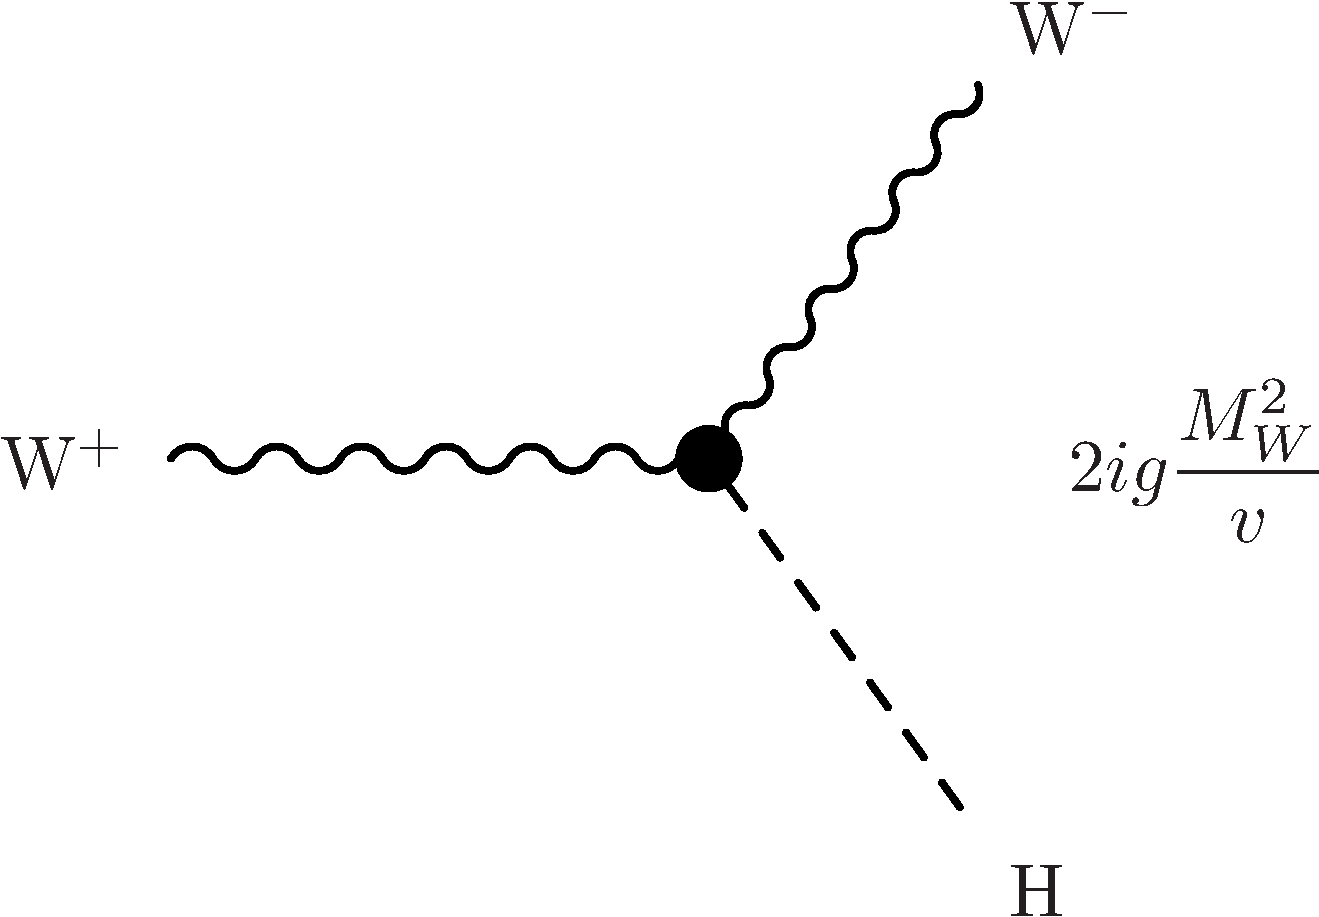
\includegraphics[width=0.3\textwidth]{\chtwo/Higgs_WWH_2.pdf}\hspace{0.4cm}
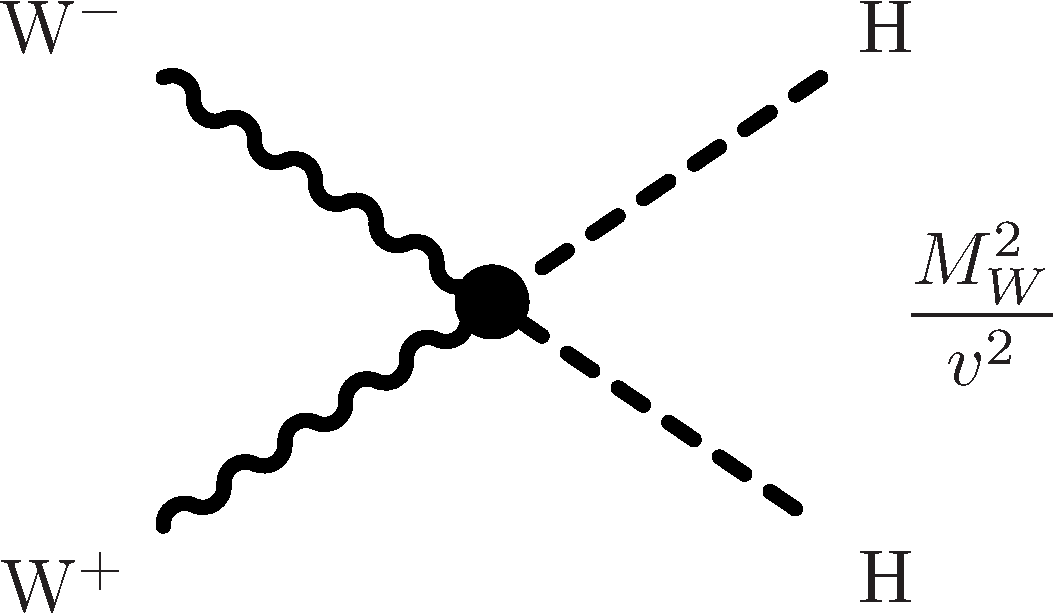
\includegraphics[width=0.3\textwidth]{\chtwo/Higgs_WWHH.pdf}\hspace{0.4cm}
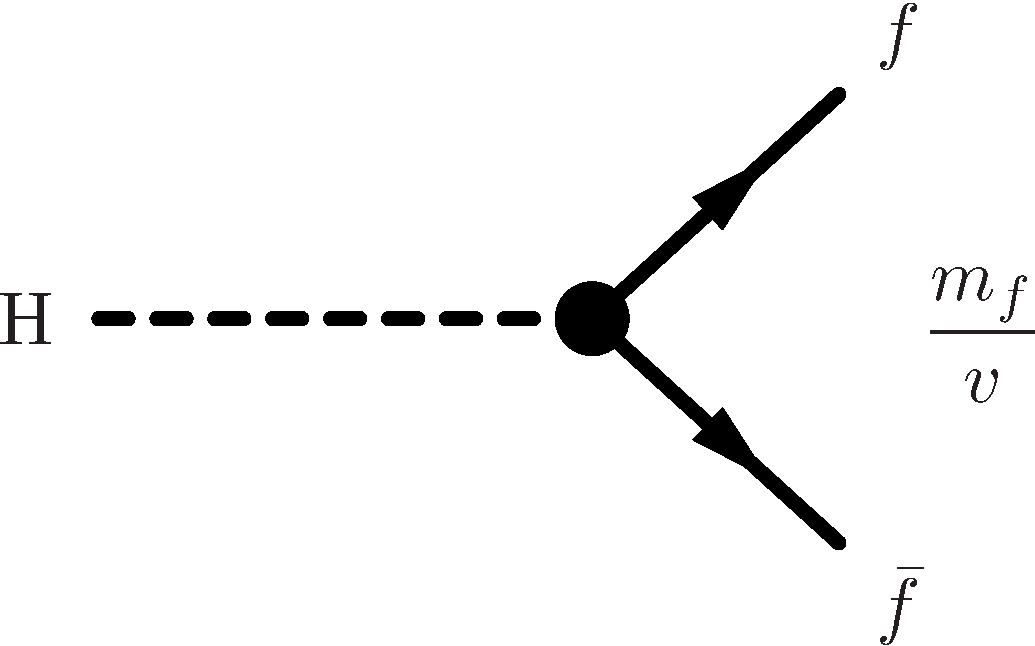
\includegraphics[width=0.3\textwidth]{\chtwo/Higgs_ffH.pdf}\\ \vspace{0.4cm}
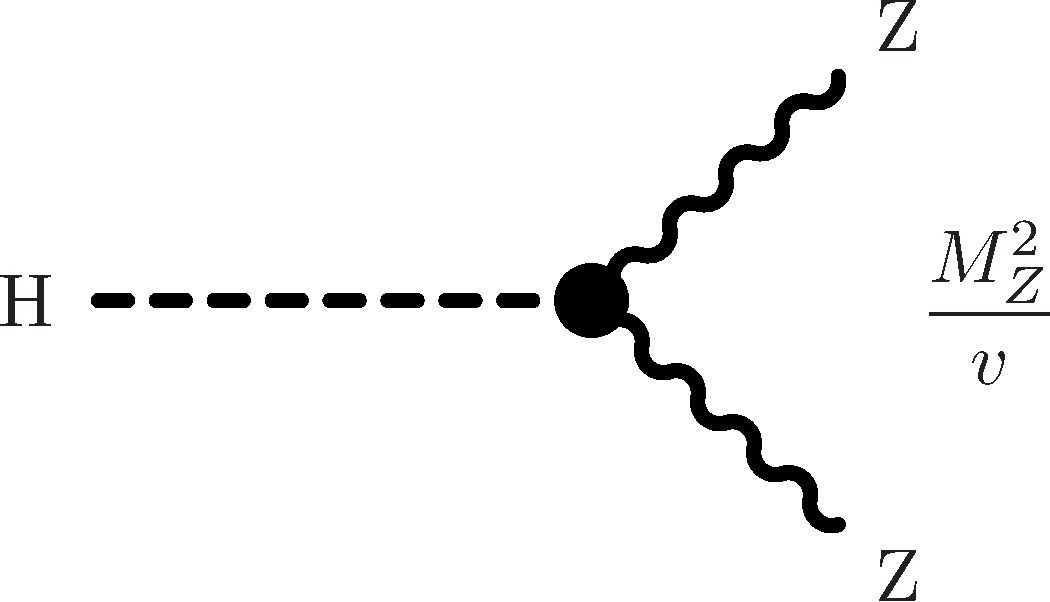
\includegraphics[width=0.3\textwidth]{\chtwo/Higgs_ZZH_2.pdf}\hspace{0.4cm}
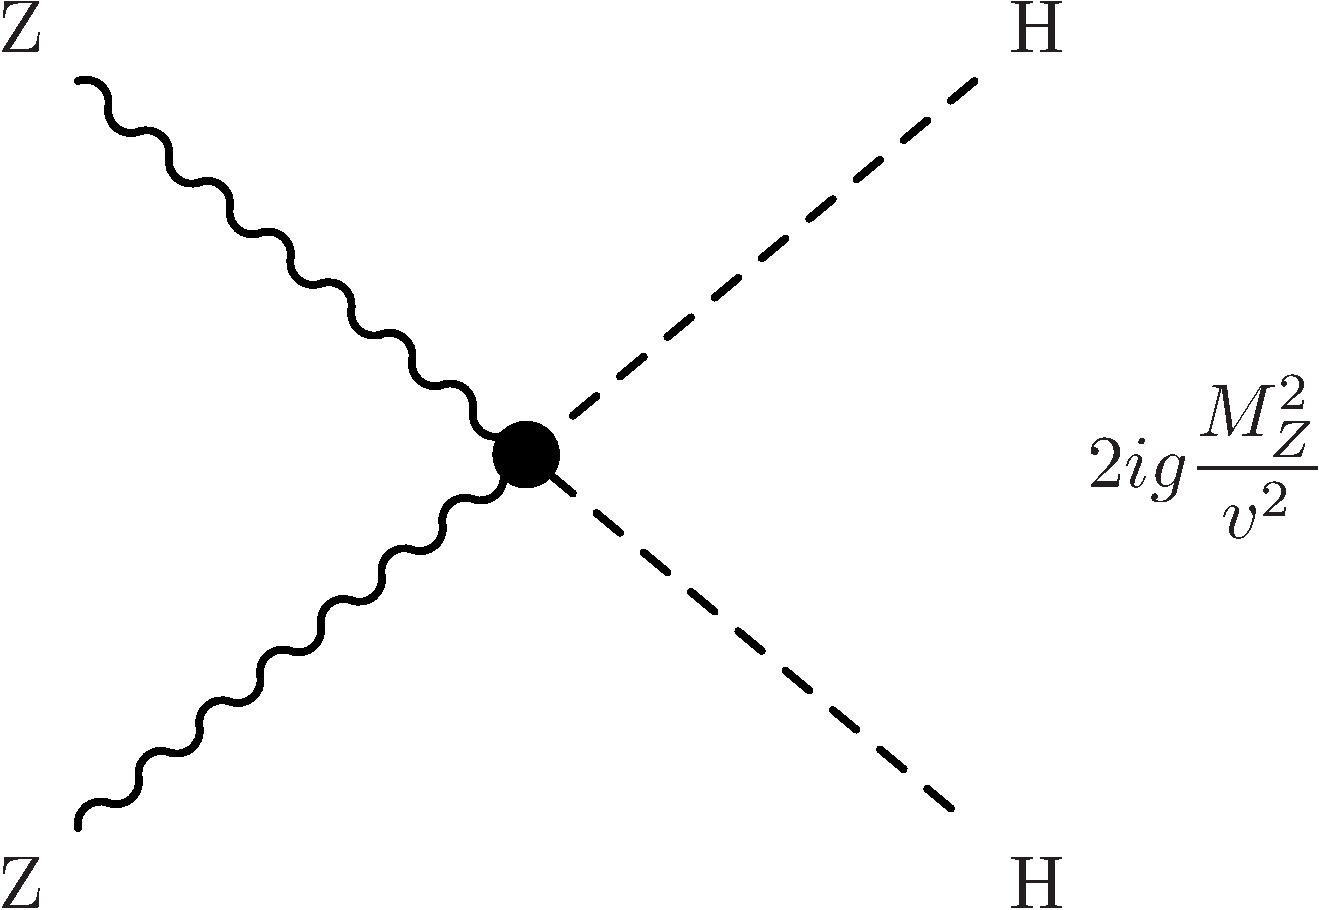
\includegraphics[width=0.3\textwidth]{\chtwo/Higgs_ZZHH.pdf}

\includegraphics[width=0.3\textwidth]{\chtwo/blank.png}\\ \vspace{0.4cm}
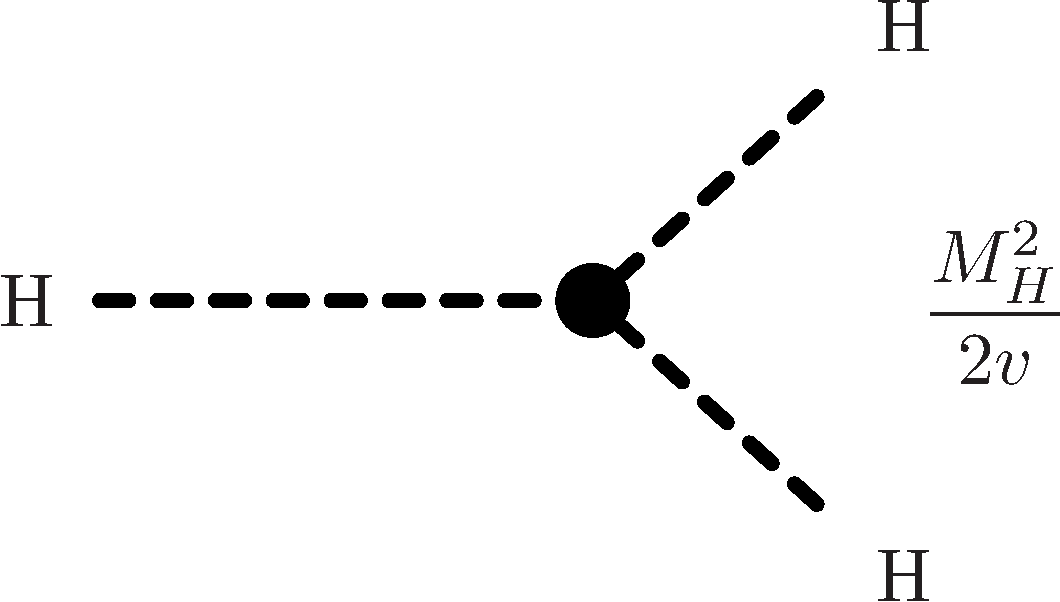
\includegraphics[width=0.3\textwidth]{\chtwo/Higgs_HHH.pdf}\hspace{0.4cm}
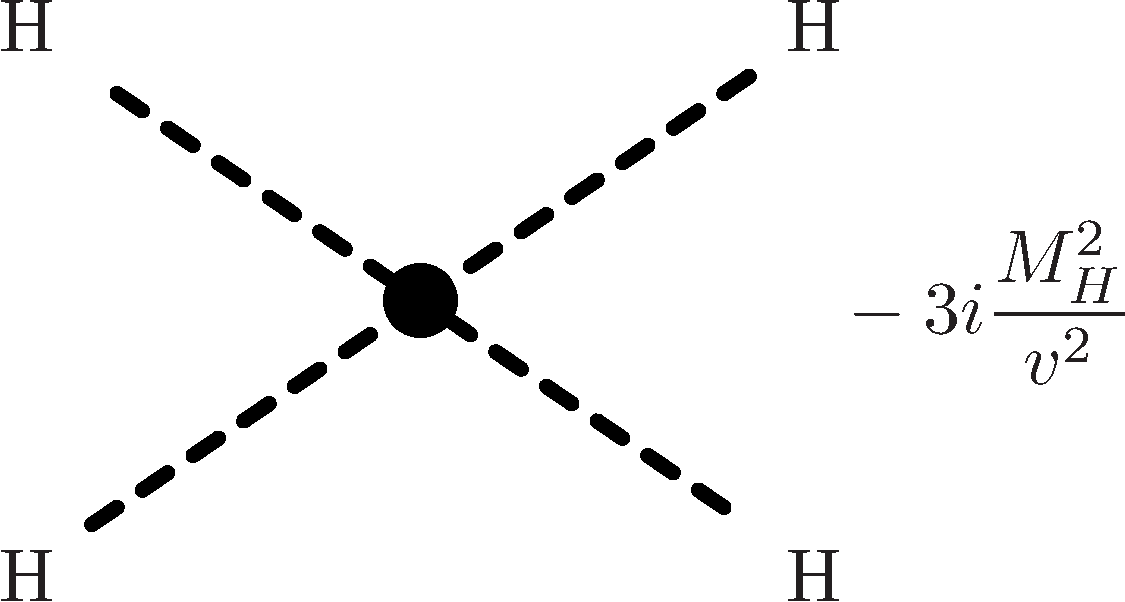
\includegraphics[width=0.3\textwidth]{\chtwo/Higgs_HHHH.pdf}

\includegraphics[width=0.3\textwidth]{\chtwo/blank.png}\\
\caption{Higgs interaction vertices in the standard model.}
\label{fig:HiggsSM}
\end{figure}

%Since, $\bar{\mathbf{f}}^\prime_L\mathbf{f}^\prime_L = \mathbf{f}_L\mathbf{f}_L$ and $\bar{\mathbf{f}}^\prime_R\mathbf{f}^\prime_R = \mathbf{f}_R\mathbf{f}_R$ ($f = u, d, \ell$),
%the form of the neutral-current part of the $\mathrm{SU(2)_L\times U(1)_Y}$ Lagrangian does not change when expressed in terms of mass eigenstates.
%Therefore, there are no flavor-changing neutral currents in the SM. %(GIM mechanism [4]).
%This is a consequence of treating all equal-charge fermions on the same footing.
%However, $\bar{\mathbf{u}}^\prime_L\mathbf{d}^\prime_L = \bar{\mathbf{u}}_L\mathbf{S}_u\mathbf{S}^\dag_d\mathbf{d}_L \equiv \bar{\mathbf{u}}_L\mathbf{V}\mathbf{d}_L$.
%In general, $\mathbf{S}_u \neq \mathbf{S}_d$; thus if one writes the weak eigenstates in terms of mass eigenstates, a $3\times3$ unitary mixing matrix $\mathbf{V}$, called the Cabibbo-Kobayashi-Maskawa (CKM) matrix\cite{CKM}, appears in the quark charged-current sector and couples any up-type quark with all down-type quarks:
%
%\begin{equation}\label{eqn:SM_e45}
%\begin{pmatrix}
%d^\prime \\ s^\prime \\ b^\prime
%\end{pmatrix}
%= \mathbf{V}
%\begin{pmatrix}
%d \\ s \\ b
%\end{pmatrix}_L
%=
%\begin{pmatrix}
%V_{ud} & V_{us} & V_{ub}\\
%V_{cd} & V_{cs} & V_{cb}\\
%V_{td} & V_{ts} & V_{tb}
%\end{pmatrix}
%\begin{pmatrix}
%d \\ s \\ b
%\end{pmatrix}_L
%\end{equation}
%
%The absolute values of its entries can be measured independently, but most precisely determined by a global fit that uses all available measurements.
%Requiring three generations of quarks and unitarity of the matrix yields the following absolute values~\cite{Olive:2016xmw,Hocker:2001xe,Charles2005}:
%
%\begin{equation}\label{eqn:SM_e46}
%\begin{pmatrix}
%0.97434^{+0.00011}_{-0.00012} & 0.22506 \pm 0.00050 & 0.00357 \pm 0.00015\\
%0.22492 \pm 0.00050                 & 0.97351 \pm 0.00013 & 0.0411 \pm 0.0013\\
%0.00875^{+0.00032}_{-0.00033} & 0.0403 \pm 0.0013    & 0.99915 \pm 0.00005
%\end{pmatrix}
%\end{equation}
%
%One observes large couplings close to 1 within the same generation (diagonal entries) whereas the off-diagonal entries are significantly smaller.
%With three quark generations, the unitarity requirement and taking into account that the quark phases cannot be measured the number of independent parameters of the matrix is reduced to four: three mixing angles between the quark generations and one complex phase that accounts for CP violation. Analogously, there exists a matrix describing the leptonic mixing, the Pontecorvo-Maki-Nakagawa-Sakata (PMNS) matrix~\cite{Ziro,PONTECORVO1968630}. It also contains four independent parameters if one assumes that neutrinos are not Majorana particles.

%%%%%%%%%%%%%%%%%%%%%%%%%%%%%%%%%%%%%%
\subsection{Observation of a particle compatible with the standard model Higgs boson}\label{subsec:HiggsLHC}
%%%%%%%%%%%%%%%%%%%%%%%%%%%%%%%%%%%%%%

The SM Higgs boson production cross sections at a proton-proton collider is shown in Fig.~\ref{fig:HiggsXS_a} as a function of the Higgs mass hypothesis and for the different leading production mechanisms.
In addition, in Fig.~\ref{fig:HiggsProd}, the corresponding Leading Order (LO) Feynman diagrams are shown.
Gluon fusion process ($gg \to \PH$) is the dominating Higgs production mechanism over the entire mass range accessible at the LHC.
In the vector boson fusion process  ($\mathrm{qq}^\prime \to \mathrm{qq}^\prime \PH$), which is about one order of magnitude weaker than gluon fusion, the Higgs boson is produced through a direct coupling with vector bosons (\PW or \PZ), which are irradiated by a pair of incoming quarks from the proton beams. 
The associated production with a \PW or \PZ boson ($\mathrm{q\bar{q}}^\prime \to \PW\PH$, $\qqbar \to \PZ\PH$) have a smaller cross section than the previous mechanisms but, the presence of the vector boson helps in reconstructing the events reducing the contamination from other SM processes.
The associated production with \ttbar pairs (qq, $gg \to \ttbar\PH$) has the smallest cross section, however, it allows for a direct access to the Higgs coupling to top quarks, representing thus an important process.
Depending on the Higgs boson mass hypothesis, different decay channels (Fig.~\ref{fig:HiggsXS_b}) can be exploited to detect it.
The Higgs boson does not couple to photons and gluons at LO, but such processes can arise via fermion or vector boson loops, giving a sizable contribution in the low mass region.\\

\begin{figure}[!htb]
\centering
\subfigure[]{\label{fig:HiggsXS_a}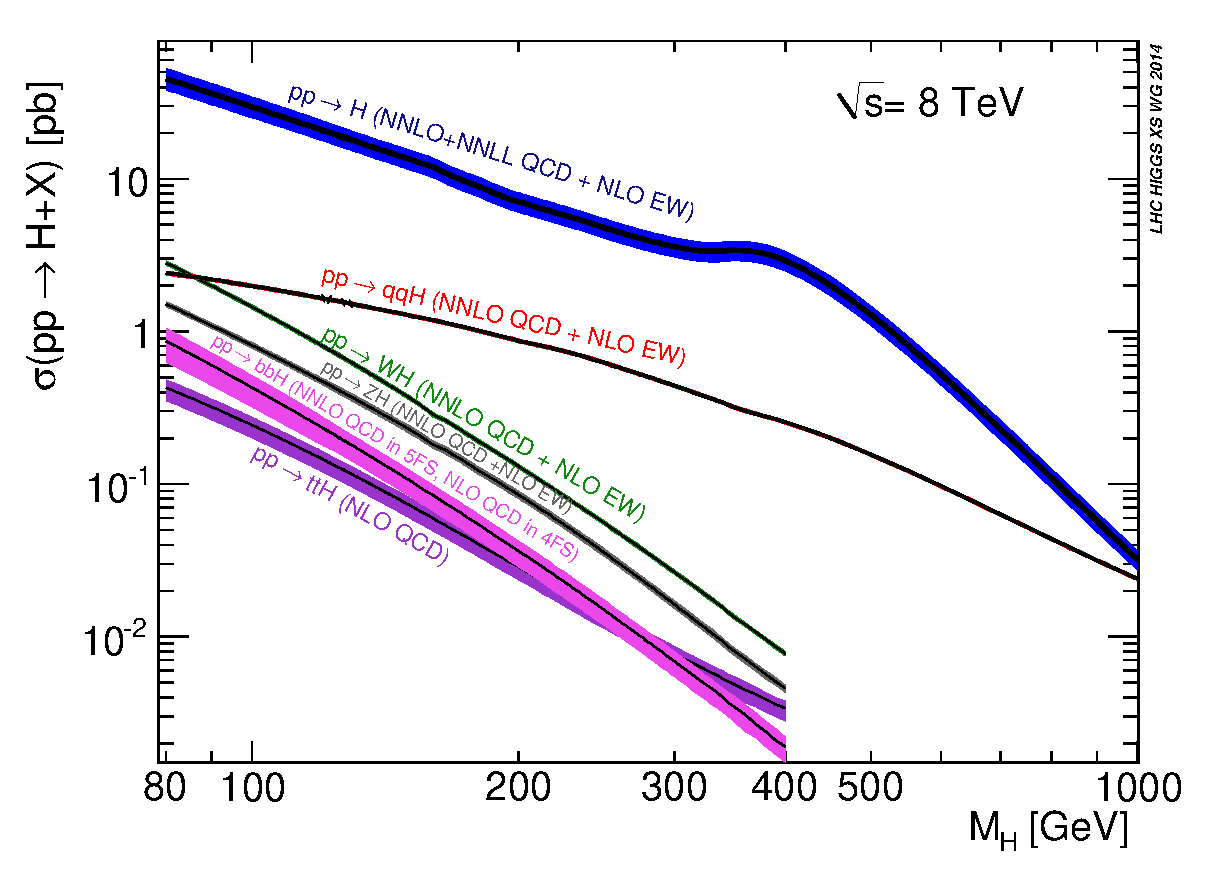
\includegraphics[width=0.56\textwidth]{\chtwo/XS_8TeV.eps}}
\subfigure[]{\label{fig:HiggsXS_b}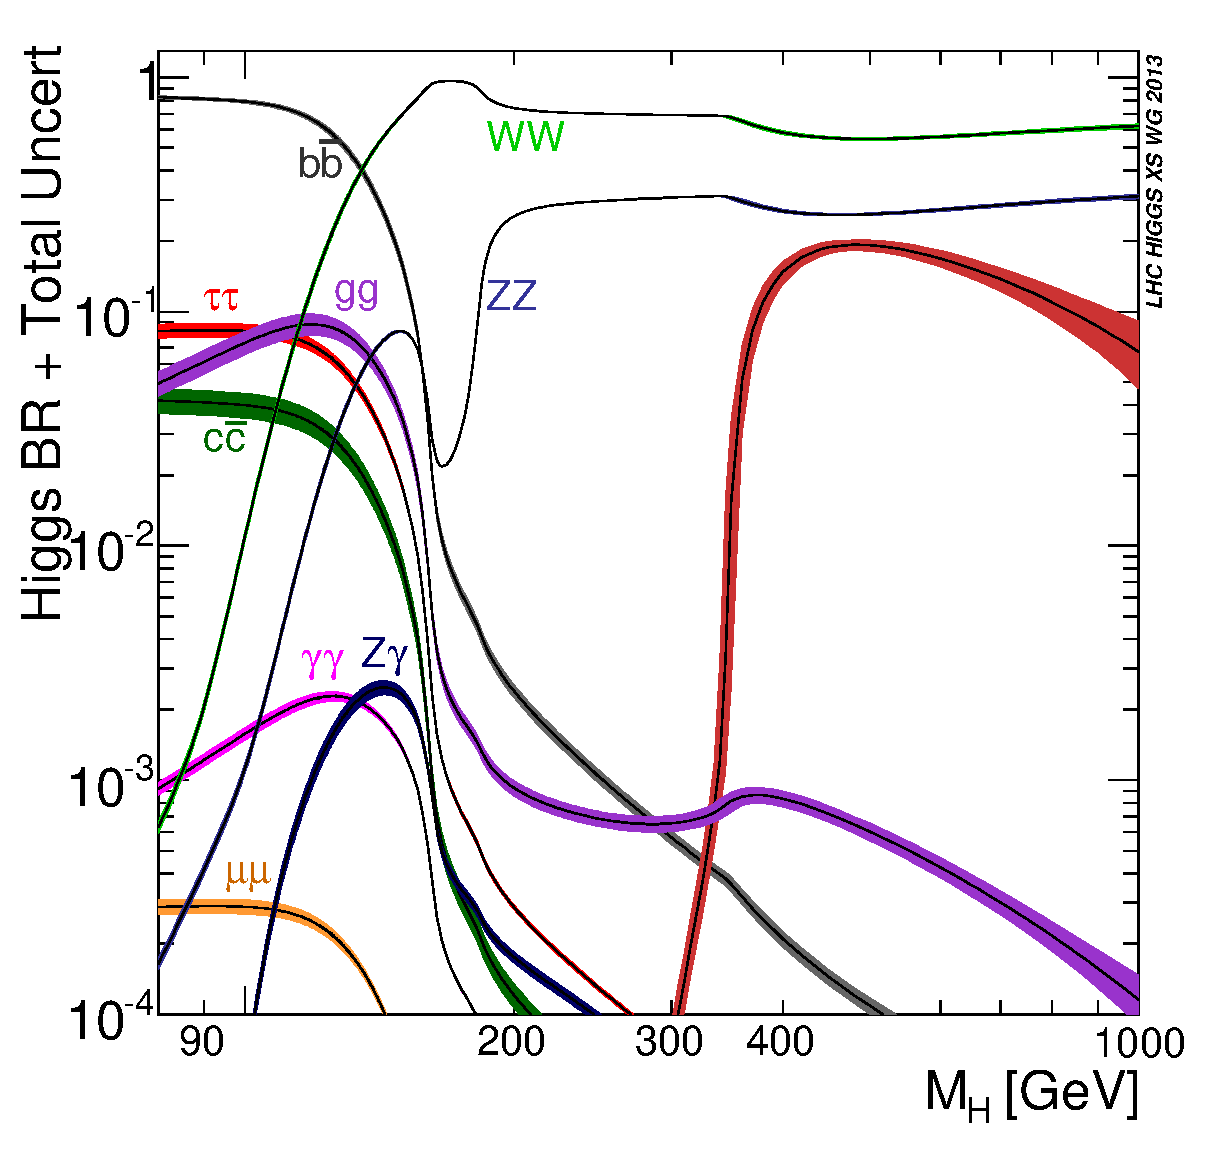
\includegraphics[width=0.42\textwidth]{\chtwo/Higgs_BR.eps}}
\caption{(a) The SM Higgs production cross-sections at $\sqrt{s} = 8\TeV$ for the different production mechanisms~\cite{Dittmaier:2011ti}. (b) Decay branching ratios of the SM Higgs boson in the different channels as a function of the mass hypothesis~\cite{Dittmaier:2011ti}.}
\label{fig:HiggsXS}
\end{figure}

\begin{figure}[!htb]
\centering
\subfigure[]{\label{fig:HiggsProd_a}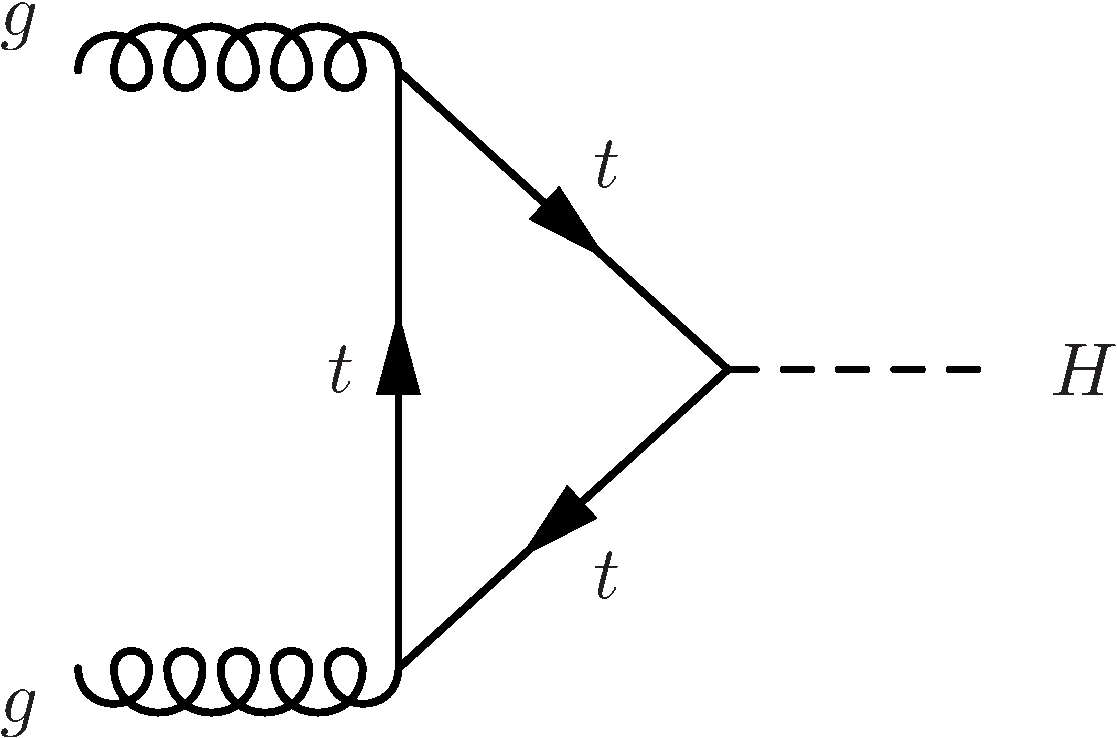
\includegraphics[width=0.23\textwidth]{\chtwo/Higgs_GF.pdf}}
\subfigure[]{\label{fig:HiggsProd_b}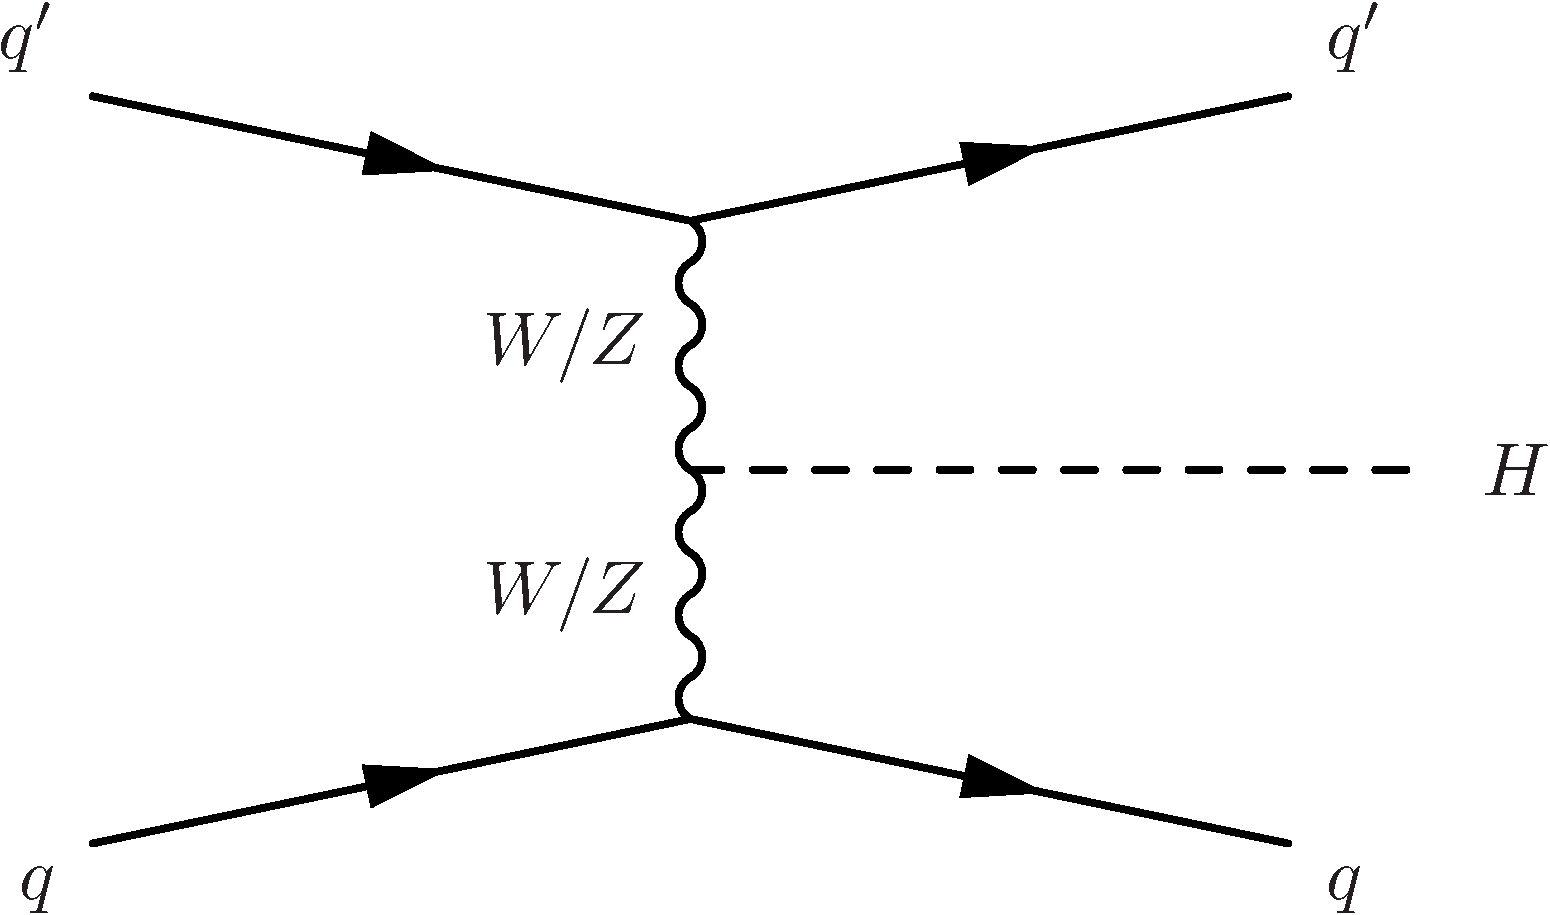
\includegraphics[width=0.23\textwidth]{\chtwo/Higgs_VBF.pdf}}
\subfigure[]{\label{fig:HiggsProd_c}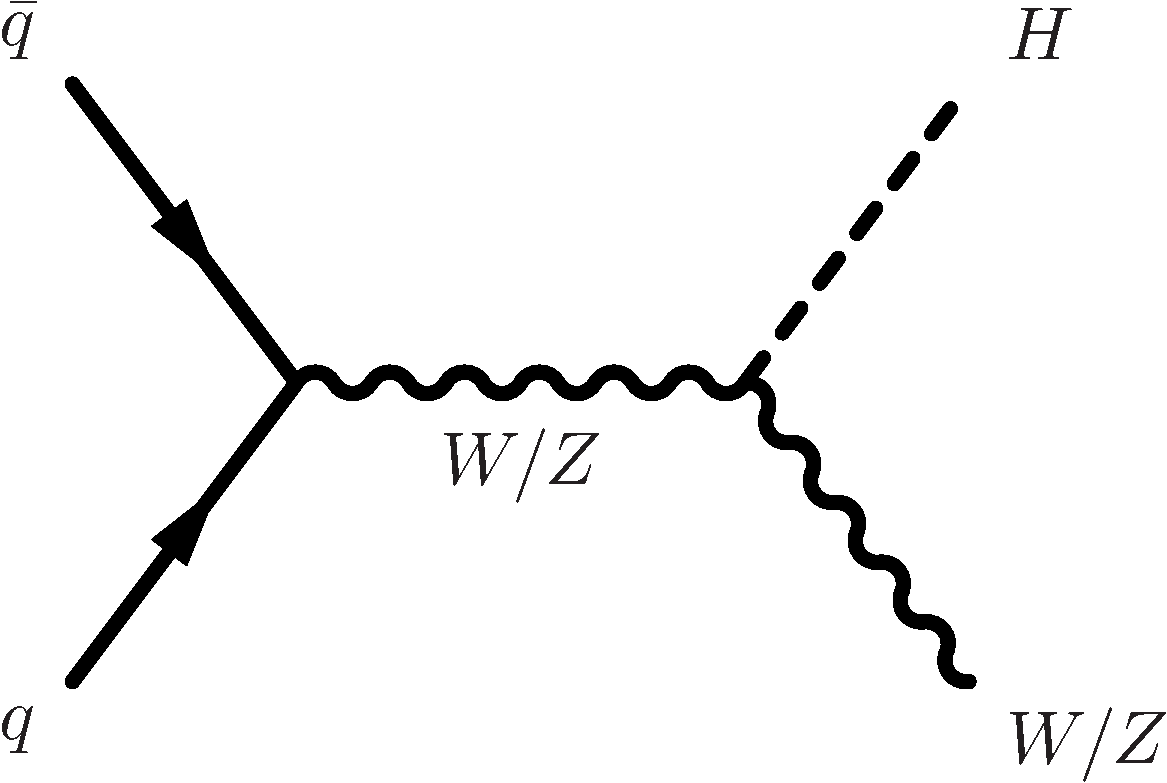
\includegraphics[width=0.23\textwidth]{\chtwo/Higgs_VH.pdf}}
\subfigure[]{\label{fig:HiggsProd_d}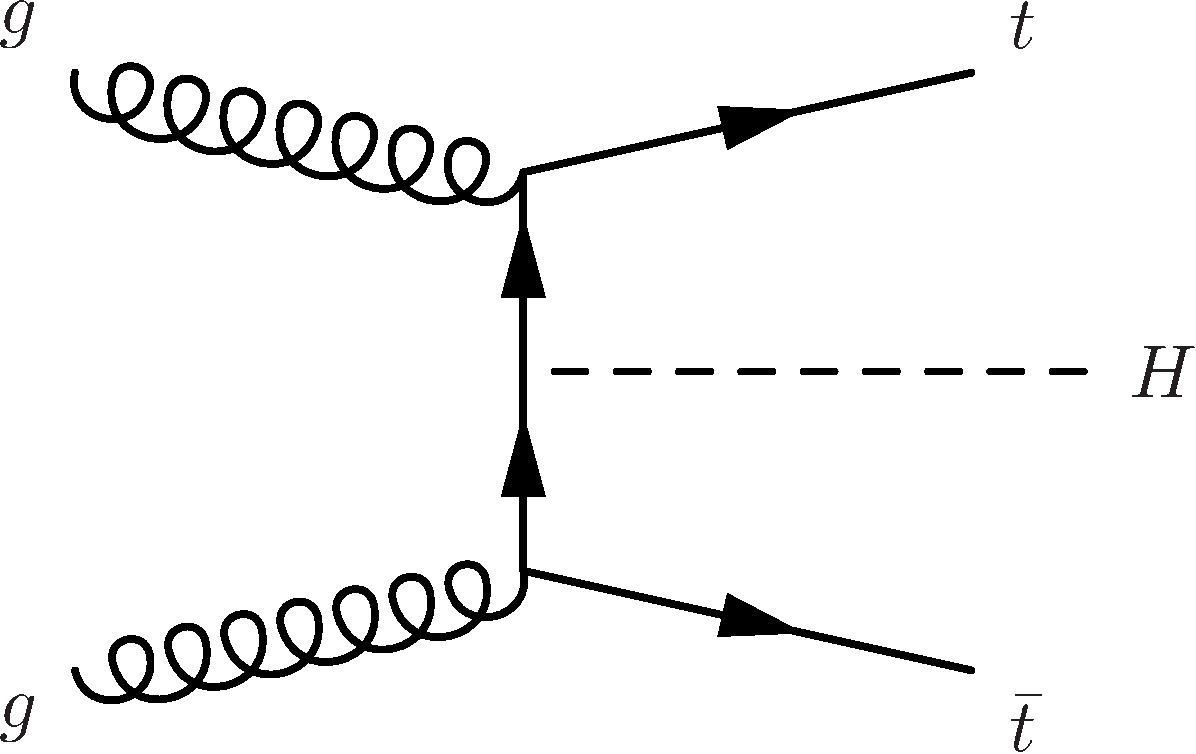
\includegraphics[width=0.23\textwidth]{\chtwo/Higgs_ttH.pdf}}
\caption{Leading order Feynman diagrams for the most important production processes of the SM Higgs boson: (a) gluon fusion, (b) vector boson fusion, (c) Higgs-strahlung and (d) \ttbar associated production.}
\label{fig:HiggsProd}
\end{figure}

The search for the massive Higgs boson has been long and tedious. 
However, in Summer 2012, the ATLAS and the CMS collaborations announced the observation of a new particle in data taken in 2011 and 2012~\cite{Chatrchyan:2013lba,Aad:2012tfa}.
A combination of the measurements targeting its decay into fermions ($\bbbar$, $\tau\tau$) or vector bosons ($\PZ\PZ^*$, $\PW\PW^*$, $\gamma\gamma$) and all the different production modes, led to an excess of events above the expected background around a mass of 125\GeV.
The CMS result yields a local significance of $5.0\sigma$ with a global significance of $4.6\sigma$ in the Higgs mass search range of $115 < m_\PH < 130\GeV$ (Fig.~\ref{fig:HiggsPvalue_a}).
For ATLAS, the local significance is found to be $5.9\sigma$ with a global significance of $5.1\sigma$ in the range $100 < m_\PH < 600\GeV$ (Fig.~\ref{fig:HiggsPvalue_b}).
A simultaneous fit to the reconstructed invariant mass peaks in the two channels with the highest mass resolution, $\PH \to \PZ\PZ^* \to 4\ell$ and $\PH \to \gamma\gamma$ , and for the two experiments has been performed.
The resulting combined measured mass of the Higgs boson is $m_\PH = 125.09 \pm 0.21 \mbox{(stat.)} \pm 0.11 \mbox{(syst.)} \GeV$ (Fig.~\ref{fig:HiggsMass})~\cite{Aad:2015zhl}.
Subsequent studies on production and decay rates~\cite{Khachatryan:2016vau} and spin-parity~\cite{Aad:2015mxa,Chatrchyan:2012jja,Khachatryan:2014kca} of the new boson showed that its properties are compatible with those expected for the SM Higgs boson. 

  \begin{figure}[!htb]
  \centering
  \subfigure[]{\label{fig:HiggsPvalue_a}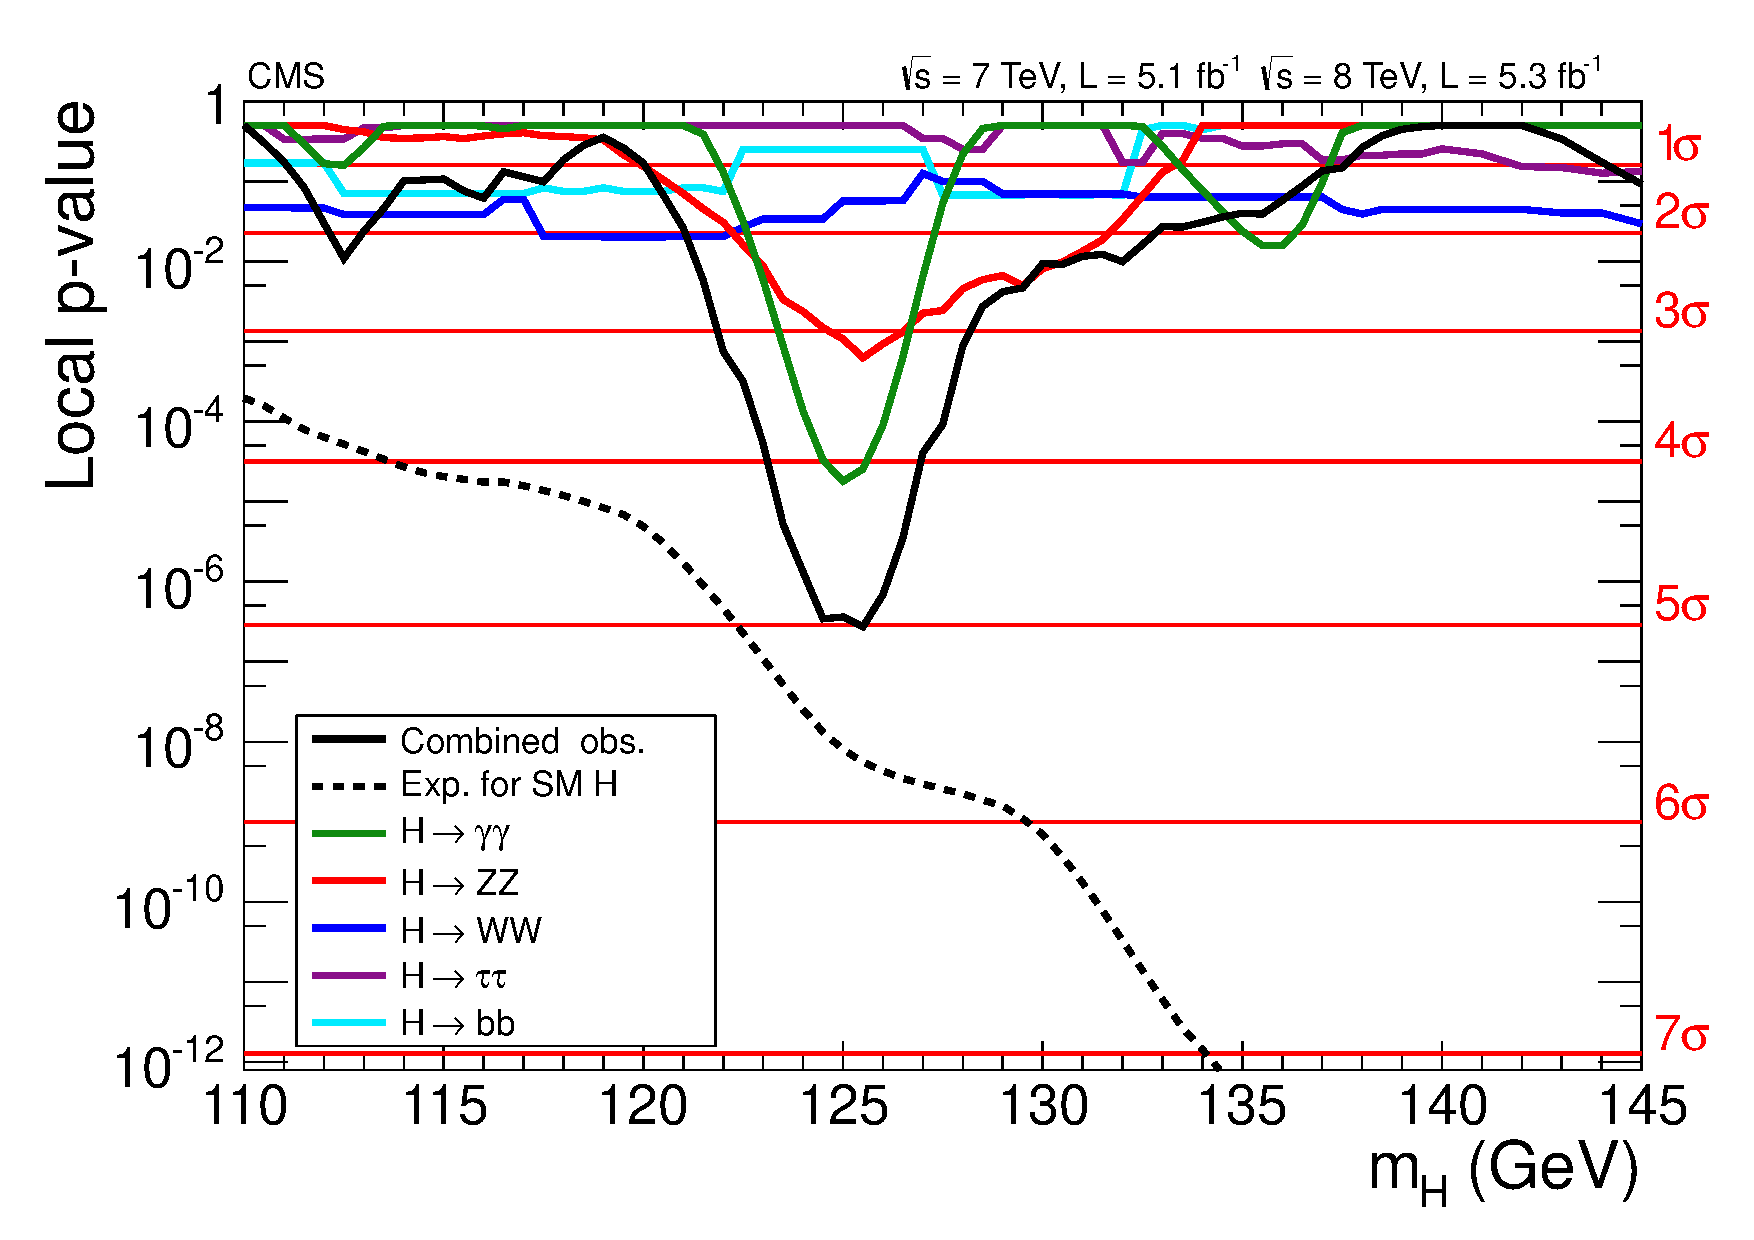
\includegraphics[width=0.45\textwidth]{\chtwo/rect_pvala_all_bydecay_smallGGScale_wideX.pdf}}
  \subfigure[]{\label{fig:HiggsPvalue_b}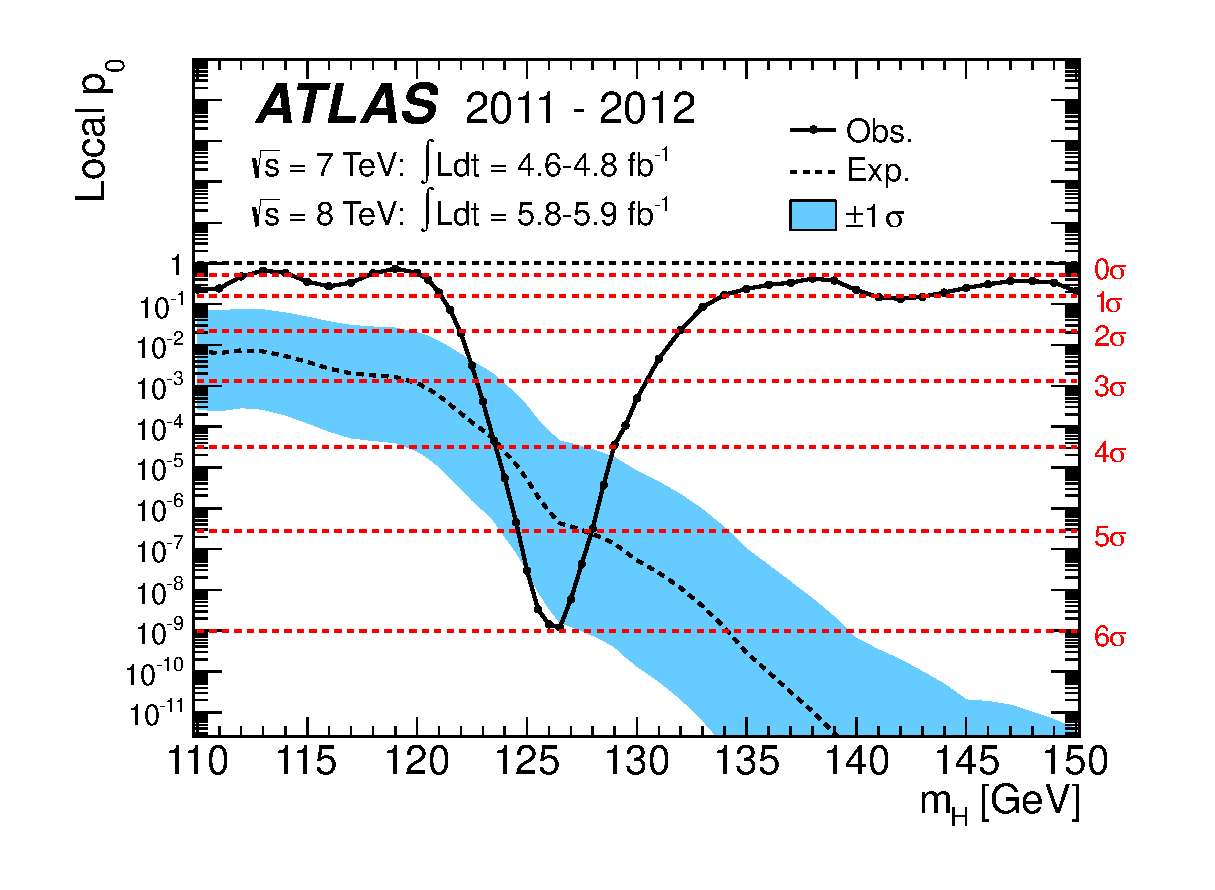
\includegraphics[width=0.45\textwidth]{\chtwo/HiggsDiscovery_ATLAS_pvalue.eps}}
  \caption{The observed (solid) local p-value as a function of the Higgs boson mass $m_\PH$ for (a) the CMS and (b) ATLAS experiments. In (a) the results for each individual channel are also shown. 
  The dashed curve shows the expected local p-value under the hypothesis of a SM Higgs boson signal at that mass.
  The horizontal red lines indicate the p-values corresponding to significances of 1 to 6$\sigma$.}
  \label{fig:HiggsPvalue}
\end{figure} 

  \begin{figure}[!htb]
  \centering
  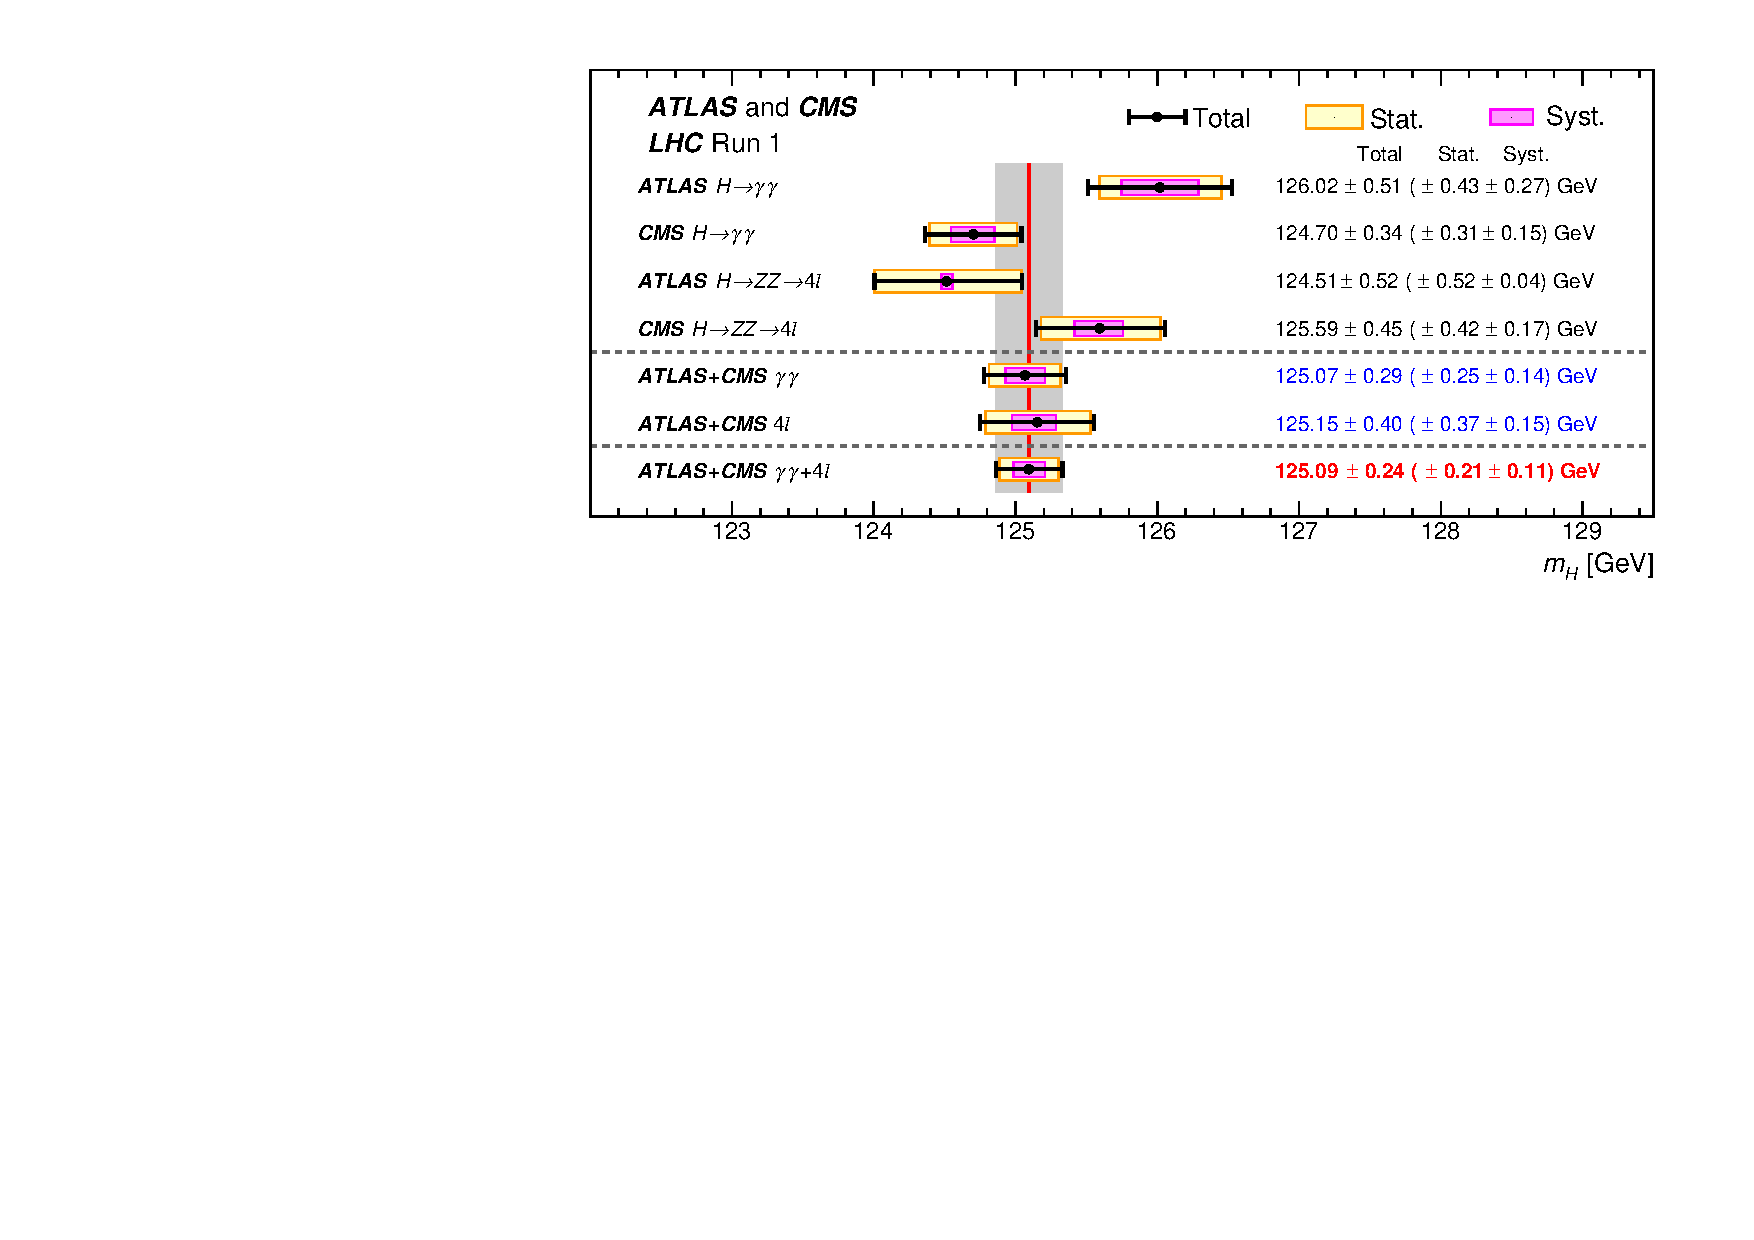
\includegraphics[width=0.7\textwidth]{\chtwo/LHC_combined_obs_unblind_summary_a1_final.pdf}
  \caption{Summary of Higgs boson mass measurements from the individual analyses of ATLAS and CMS and from their combination.
  The magenta and yellow bands correspond to the the systematic and statistical uncertainties, respectively. The total uncertainties are also indicated as black error bars.
  The red vertical line and corresponding gray shaded column indicate the central value and the total uncertainty of the combined measurement, respectively~\cite{Aad:2015zhl}.}
  \label{fig:HiggsMass}
\end{figure} 

Finally, the Higgs boson couplings to SM particles are investigated simultaneously in different production and decay processes, including the possibility of the Higgs boson to be coupled to BSM particles~\cite{Khachatryan:2016vau}.
To test possible deviations from the SM predictions, the coupling modifiers, $k^2_j = \sigma_j/\sigma^\mathrm{SM}_j$ and $k^2_j = \Gamma_j/\Gamma^\mathrm{SM}_j$, for production and decay rates, are introduced. 
However, to directly measure the individual coupling modifiers, an assumption about the Higgs boson width $\Gamma_\PH$ is necessary. Thus, another modifier is introduced and defined as $k_\PH = \sum_j \mathcal{B}^\mathrm{SM}_jk^2_j$, where $\mathcal{B}^\mathrm{SM}_j$ are the branching fractions for the Higgs boson decay to the final state $f$ as predicted by the SM. In the case where the SM decays of the Higgs boson are the only ones allowed,
the relation $k^2_\PH = \Gamma_\PH/\Gamma^\mathrm{SM}_\PH$ holds. If instead deviations from the SM are introduced in the decays, the width can be expressed as:

\begin{equation}\label{eqn:SM_e45}
\Gamma_\PH = \frac{k^2_\PH\Gamma^\mathrm{SM}_\PH}{1 - B_\mathrm{BSM}},
\end{equation}

\noindent where $B_\mathrm{BSM}$ indicates the total branching fraction into BSM decays.
The two possible scenarios are considered: the first leaves $B_\mathrm{BSM}$ free, provided that $B_\mathrm{BSM} \geq 0$, whereas the second assumes $B_\mathrm{BSM} = 0$. 
The parameters of interest in the fits to data are thus the seven independent coupling modifiers, $k_\PZ$, $k_\PW$, $k_\mathrm{t}$, $k_\tau$, $k_\mathrm{b}$, $k_g$, and $k_\gamma$, 
one for each SM particle involved in the production processes and decay modes studied, plus $B_\mathrm{BSM}$ in the case of the first scenario.
The results of the two fits are shown in Fig.~\ref{fig:HiggsCoupl}.
The overall branching fraction of the Higgs boson into BSM decays is determined to be less than 34\% at 95\% CL.
This constraint applies to invisible decays into BSM particles, decays into BSM particles that are not detected as such, and modifications of the decays into SM particles that are not directly measured by the experiments.

  \begin{figure}[!htb]
  \centering
  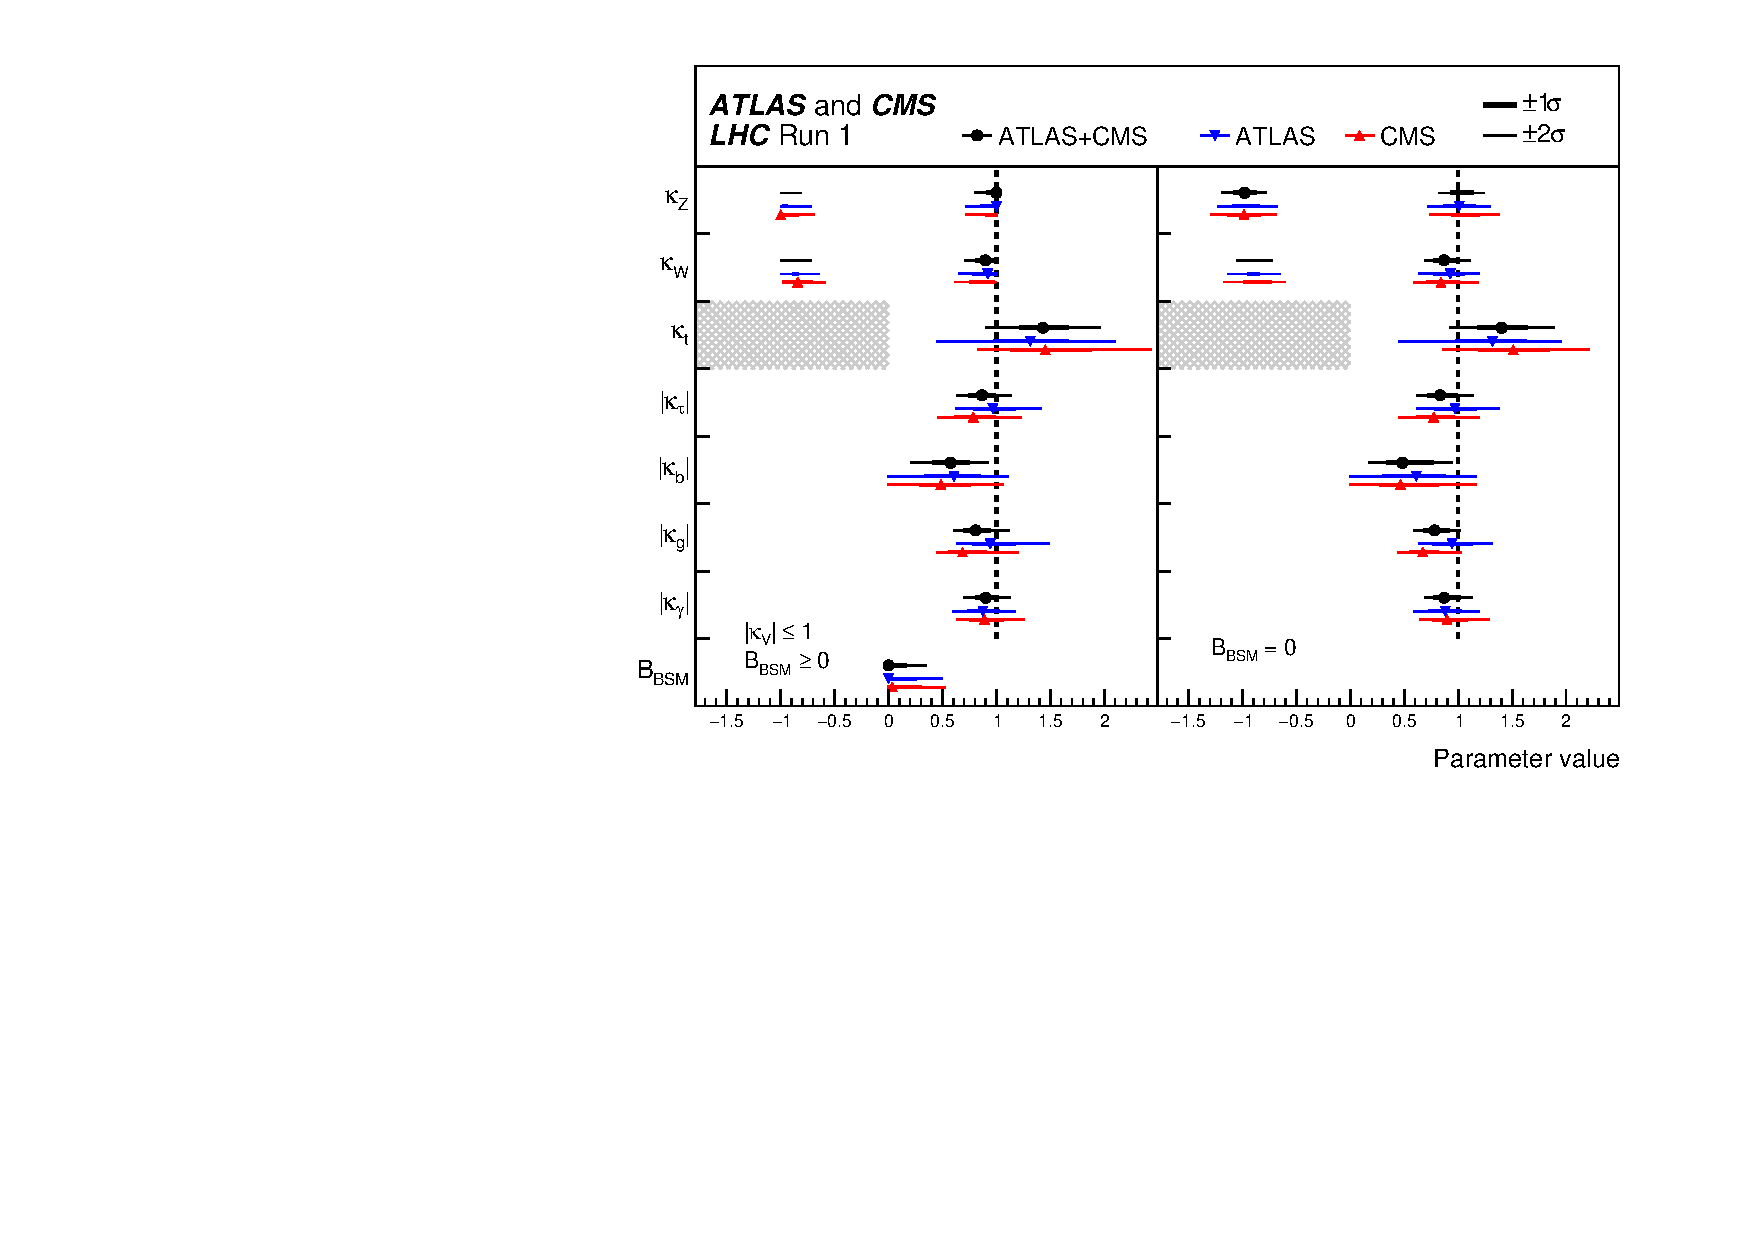
\includegraphics[width=0.7\textwidth]{\chtwo/plot_K2_K2_BRinv_per_exp_merged.pdf}
  \caption{Fit results for two parameterizations: the first one assumes that $B_\mathrm{BSM} \geq 0$, and the second one assumes that there are no additional BSM contributions to the Higgs boson width ($B_\mathrm{BSM} = 0$). The measured results for the combination of ATLAS and CMS are reported together with their uncertainties, as well as the individual results from each experiment~\cite{Aad:2015zhl}.}
  \label{fig:HiggsCoupl}
\end{figure} 

%%%%%%%%%%%%%%%%%%%%%%%%%%%%%%%%%%%%%%%%%
\subsection{Quantum chromodynamics}\label{subsec:QCD}
%%%%%%%%%%%%%%%%%%%%%%%%%%%%%%%%%%%%%%%%%

Quantum Chromodynamics (QCD) is the gauge theory of strong interactions, describing the dynamics of colored quarks and gluons.
The QCD represents the $SU(3)_C$ component of the standard model, where $C$ denotes the color.
After applying the principle of gauge invariance to the free Lagrangian for the quark fields holding color $\alpha$ that runs from 1 to 3 (usually identified with red, green, blue), and flavor $q$, one obtains the following expression for the final gauge invariant QCD Lagrangian

\begin{equation}\label{eqn:SM_e46}
\mathcal{L}_\mathrm{QCD} = \sum_{q} \bar{\psi}_{q,\alpha} (i\gamma^\mu\partial_\mu\delta_{\alpha\beta} - g_s\gamma^\mu t^a_{\alpha\beta}\mathcal{A}^a_\mu - m_q\delta_{\alpha\beta})\psi_{q,b} - \frac{1}{4}G^a_{\mu\nu}G^{\mu\nu}_a.
\end{equation}

In the equation above, the quark fields are represented by the spinors $\psi$. The fields $\mathcal{A}^a_\mu$ corresponds to the eight gluon fields, since $C$ runs from 1 to $N^2_C - 1 = 8$.
Each gluon carries one unit of color and one unit of anticolor.
The eight $3\times3$ matrices $t^a_{\alpha\beta}$ are the $SU(3)_C$ generators and rotate the quark color in the $SU(3)_C$ space in a quark-gluon interaction.
The field tensor is

\begin{equation}\label{eqn:SM_e47}
G^a_{\mu\nu} = \partial_\mu\mathcal{A}^a_\nu - \partial_\nu\mathcal{A}^a_\mu - g_s f_{abc}\mathcal{A}^b_\mu\mathcal{A}^c_\nu,
\end{equation}

\noindent where $f_{abc}$ are the structure constants of the $SU(3)$ group.
As $[t^a,t^b] = if_{abc}t^c$ the group is non-Abelian. Owing this property, $G^a_{\mu\nu}G^{\mu\nu}_a$ term generates the cubic and quartic gluon self-interactions.
The fundamental parameters of QCD are the \textit{strong coupling constant} $g_s$, often written in terms of $\alpha_s = g_s^2/4\pi$, and the quark masses $m_q$.
All interactions appearing in Eq.~\ref{eqn:SM_e45} have strength given by $g_s$ (Fig.~\ref{fig:QCDVtx}).\\

\begin{figure}[!htb]
\centering
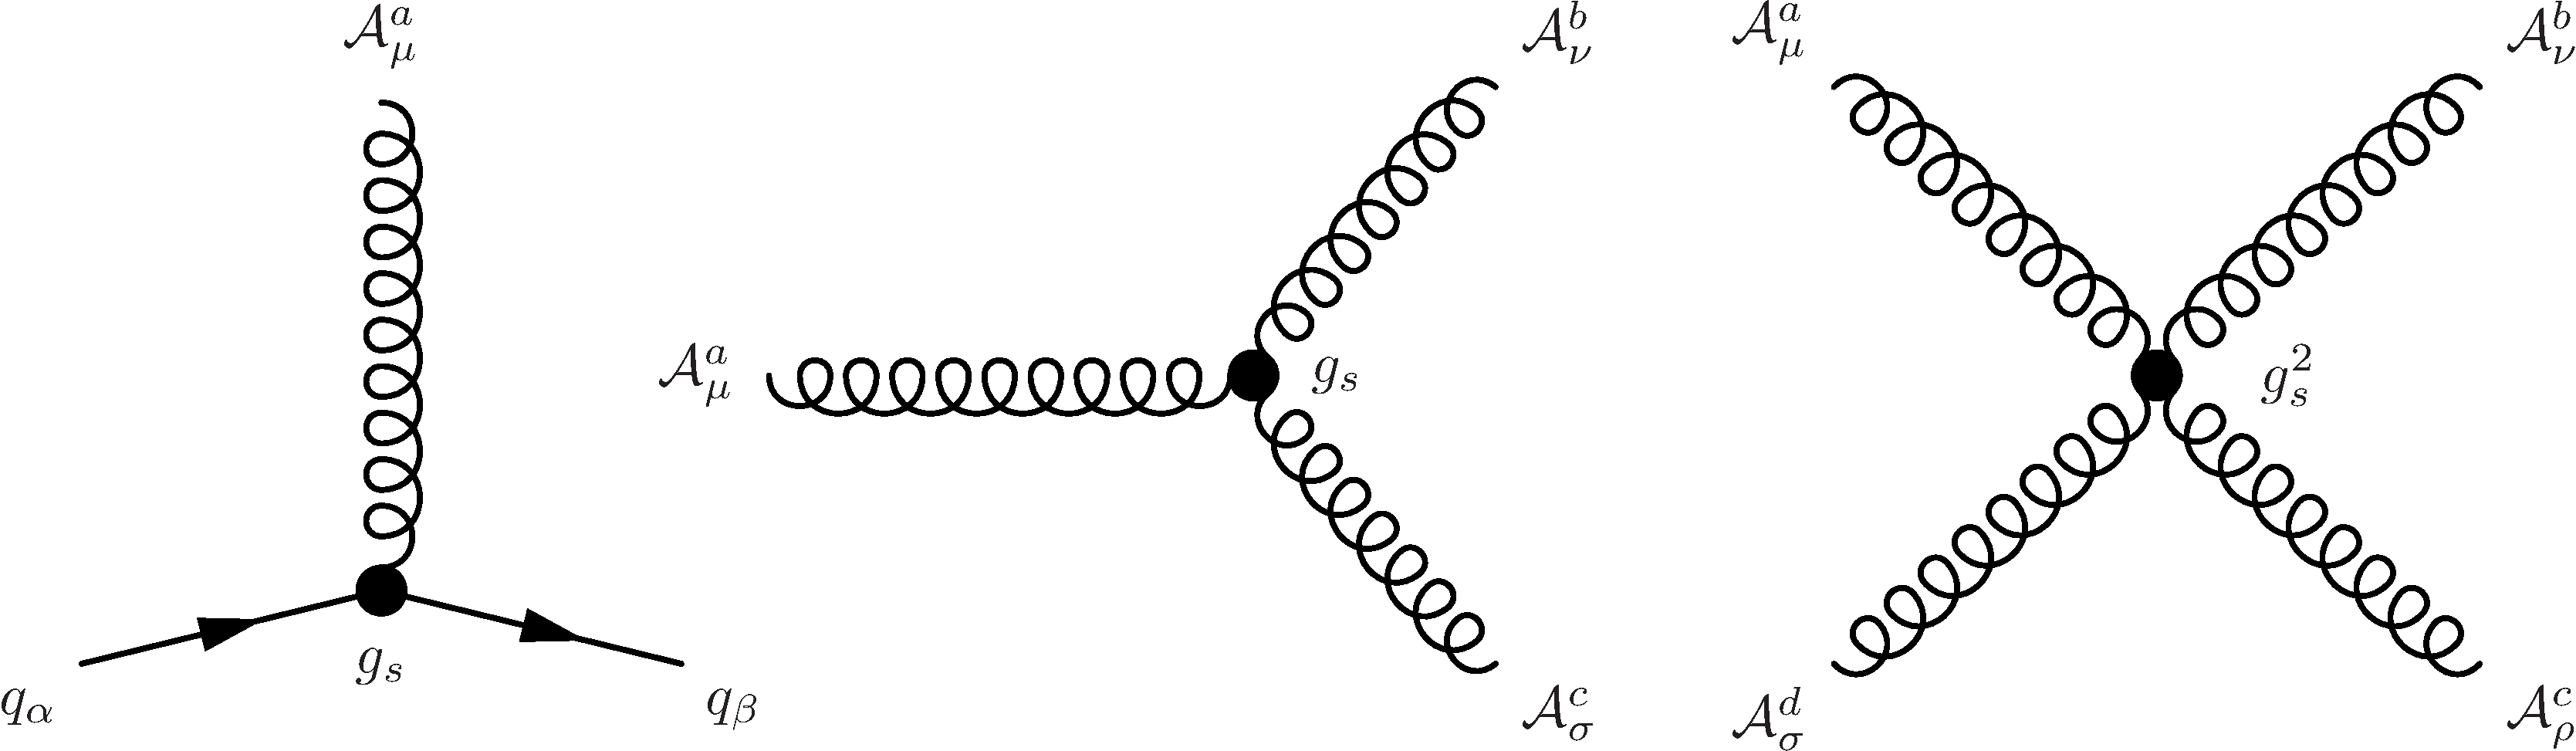
\includegraphics[width=0.9\textwidth]{\chtwo/QCD_vtx.pdf}
\caption{Interaction vertices of the QCD Lagrangian.}
\label{fig:QCDVtx}
\end{figure}

The QCD has the property of \textit{asymptotic freedom}, i.e. the coupling becomes weak at high energies or short distances, and for energies approaching zero or for very large distances, it tends to infinity.
As a consequence, the further away a quark is pulled from another one, the stronger the force gets, such that quarks cannot exist as free particles.
Because of this phenomenon, referred to as \textit{confinement}, quarks form bound color-singlet states called hadrons, consisting of either a quark and an antiquark (mesons) or three quarks or antiquarks (baryons).
%As a consequence, only in very high momentum transfer interactions, quarks can be regarded as free particles, whereas at low energy or large distance, the interaction becomes strongly coupled leading to \textit{confinement} of quarks %and gluons. Instead, they form bound color-singlet states called hadrons, consisting of either a quark and an antiquark (mesons) or three quarks or antiquarks (baryons).
%In this process, after a quark production, at very short distances, the quantum nature of QCD predicts the generation of virtual quark-antiquark (or gluons) pairs, which couple together through color strings forming observable un-%colored baryons and mesons.
In the regime of very high momentum transfer interactions, the perturbation theory is a very satisfactory description of QCD physics observables, giving precise predictions about what can be tested in collider experiments. This approach is called perturbative-QCD, or pQCD. In this framework, QCD predictions are calculated using the formalism of the Feynman rules which are derived from the $\mathcal{L}_\mathrm{QCD}$.
The transition amplitudes for a given process from a set of initial state particles to a set of final state particles are computed by sorting the diagrams by the factors of the coupling constants and calculating them up to a certain order.
However, higher order diagrams generally contain loops which contribute and lead to divergencies.
In order to obtain finite predictions for the cross sections, a renormalization of the theory is performed, resulting in a cancellation of the divergent terms.
%The divergencies are absorbed into a redefinition of the color charge. As a consequence of this, $\alpha_s$ is a running coupling constant as a function of a renormalization scale $\mu_R$, and is given by
The predictions for observables are then expressed in terms of the renormalized coupling $\alpha_s(\mu^2_R)$, a function of the renormalisation scale $\mu_R$. 
The coupling satisfies the renormalisation group equation:

\begin{equation}\label{eqn:SM_e48}
\mu^2_R\frac{\mathrm{d}\alpha_s}{\mathrm{d}\mu^2_R} = \beta(\alpha_s) = - (b_0\alpha^2_s + b_1\alpha^3_s + b_2\alpha^4_s + \dotsc)
\end{equation}

\noindent where the $b_i$ are the $i$-loop coefficients of the $\beta$ function.
They depend on the number of quark flavors $n_f$, and for sixteen or less flavors the strong coupling gets smaller for processes that involve large momentum transfer, leading to the asymptotic freedom.
Choosing $\mu_R$ close to the typical scale of the process of interest $Q^2$, the $\alpha_s(\mu_R)$ represents the effective strength of the strong interaction between particles under study.
Neglecting all the $b_i$ coefficients but $b_0$, an exact leading order expression for the running coupling $\alpha_s$ can be obtained

\begin{equation}\label{eqn:SM_e49}
\alpha_s(\mu^2_R) = \frac{1}{b_0\log \left( \frac{\mu^2_R}{\Lambda^2_\mathrm{QCD}} \right) } = \frac{12\pi}{(33-2n_f)\log \left( \frac{\mu^2_R}{\Lambda^2_\mathrm{QCD}} \right) }
\end{equation}

\noindent where $\Lambda_\mathrm{QCD}$ is the perturbative cut-off over the renormalization's integrals, and is not predicted by the theory.
The meaning of this cut-off is the validity of the perturbative regime approximation, beyond which the integrals would diverge.
For many experimental studies, the strong coupling is evaluated at a fixed energy scale, typically of the order of the electroweak scale, $\mu_R \simeq M_\PZ$ (Fig.~\ref{fig:AlphaS}).

\begin{figure}[!htb]
  \centering
  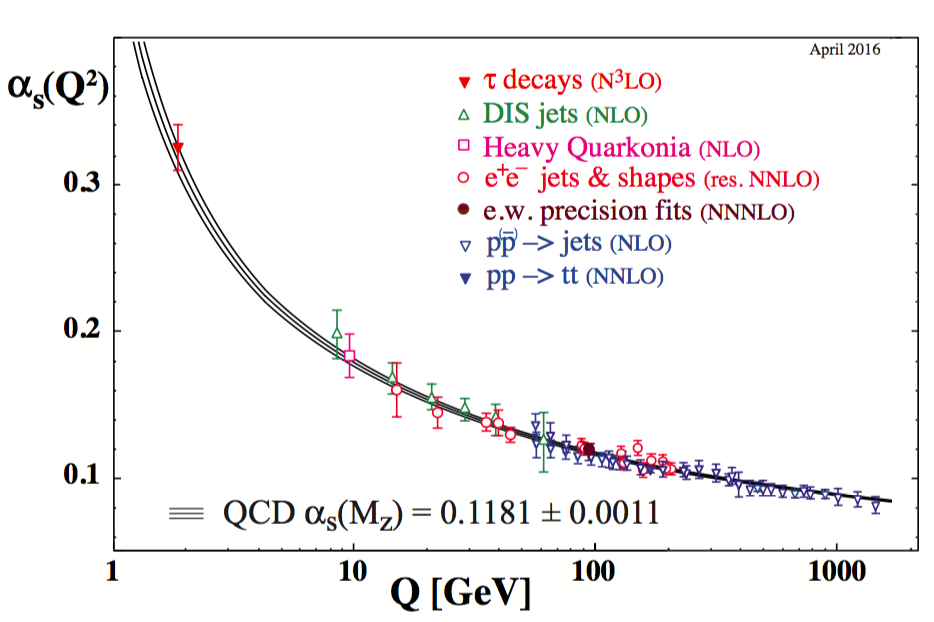
\includegraphics[width=0.6\textwidth]{\chtwo/alphaS_measurement_2016.png}
  \caption{Summary of measurements of the running coupling $\alpha_s$ as a function of the energy scale $Q$ of the process~\cite{Olive:2016xmw}.}
  \label{fig:AlphaS}
\end{figure} 

%\section{Theories of new physics}
  \section{Theories of new physics}
\label{sec:BSMintro}

The standard model of particle physics has been very successful in describing observations. 
However, as explained in the previous section, this framework leaves several unanswered fundamental questions.
Many extensions to the standard model have been proposed that attempt to address the open issues and to achieve a more fundamental theory
that could explain the entirety of current phenomena.
These new theoretical developments are referred to as \textit{beyond standard model} (BSM) theories.
In this section, three specific BSM scenarios are reviewed, which are of particular interest because of their highly predictive features.
Specifically, with the aim of addressing the hierarchy problem of the SM, they predict the existence of new resonances with masses in the TeV range,
which can be produced at hadron colliders.
Furthermore, since the new resonances can decay into pairs of well-known standard model particles, their existence and properties can be directly probe by collider experiments.
In particular, the decay modes into a pair of electroweak bosons \PW, \PZ or \PH, can provide striking signatures, as new techniques have been developed by the experiments to efficiently reconstruct the decay and mass of the bosons in the final state.

%%%%%%%%%%%%%%%%%%%%%%%%%%%%%%%%%%%%%%%%%%%%
\subsection{Warped Extra dimensions}\label{subsec:graviton}
%%%%%%%%%%%%%%%%%%%%%%%%%%%%%%%%%%%%%%%%%%%%

A class of theories beyond the standard model are those postulating the existence of new compactified spatial dimensions.
They attempt to explain the apparent weakness of gravity by assuming that SM particles are confined in a (3+1)-dimensional hypersurface called \textit{3-brane},
as opposed to gravity which is allowed to propagate in a (4+n)-dimensional \textit{bulk}.
In this scenario, the strength of gravity is diluted in the extra dimensions (thereby weakening our perception of gravity), while the other fundamental forces would not.

The basic idea comes from the so-called \textit{large extra dimensions} scenario proposed by Arkani-Hamed, Dimopoulos and Dvali (ADD model)~\cite{ArkaniHamed:1998rs}.
If spacetime has 4+$n$ dimensions, then the effective 4-dimensional (reduced) Planck scale, $\bMPl = \MPl/\sqrt{8\pi}$,
is determined by the fundamental (4+$n$)-dimensional Planck scale, $M_*$, and the geometry of the extra dimensions:

\begin{equation}\label{eqn:WED_1}
\bMPl^2 = V_nM^{n+2}_* \simeq R^nM^{n+2}_*,
\end{equation}

\noindent where $V_n$ is the volume of the $n$-dimensional compactified space and $R$ its radius.
The hierarchy problem is thus eluded if $M_* \sim 1\TeV$, which turns into a condition on the size $R$ of the extra dimensions.
Assuming $n = 1$, one can solve Eq.~\ref{eqn:WED_1} and obtain $R \sim 10^8\unit{m}$.
This is a scale of the order of the Earth-Sun distance, over which we know that the $1/r^2$ Newton's law of gravitational attraction works very well. Thus, $n = 1$ is excluded.
For $n = 2$, one obtains $R \sim 100\mum$ or $R^{-1} \sim 10^{-4}$\unit{eV}, which is close to the limit of current table top experimental searches for deviations from the Newton's law~\cite{Hoyle:2004cw}. 

The purpose of this model was to eliminate the hierarchy problem, i.e. to remove the large ratio between the weak scale $v$ and the true fundamental scale \bMPl, hence the requirement $M_* \sim 1\TeV$.
However, it introduces a new hierarchy, namely that between the compactification scale $\mu_c = 1/R$ and $v$.
Thus, the ADD really only trades one large ratio for another and does not really eliminate the hierarchy problem.
An alternative solution, represented by the so-called \textit{warped extra dimensions} (WED) scenario, has been proposed by Randall and Sundrum (RS)~\cite{Randall:1999ee}.

\begin{wrapfigure}{R}{0.4\textwidth}
 \centering
 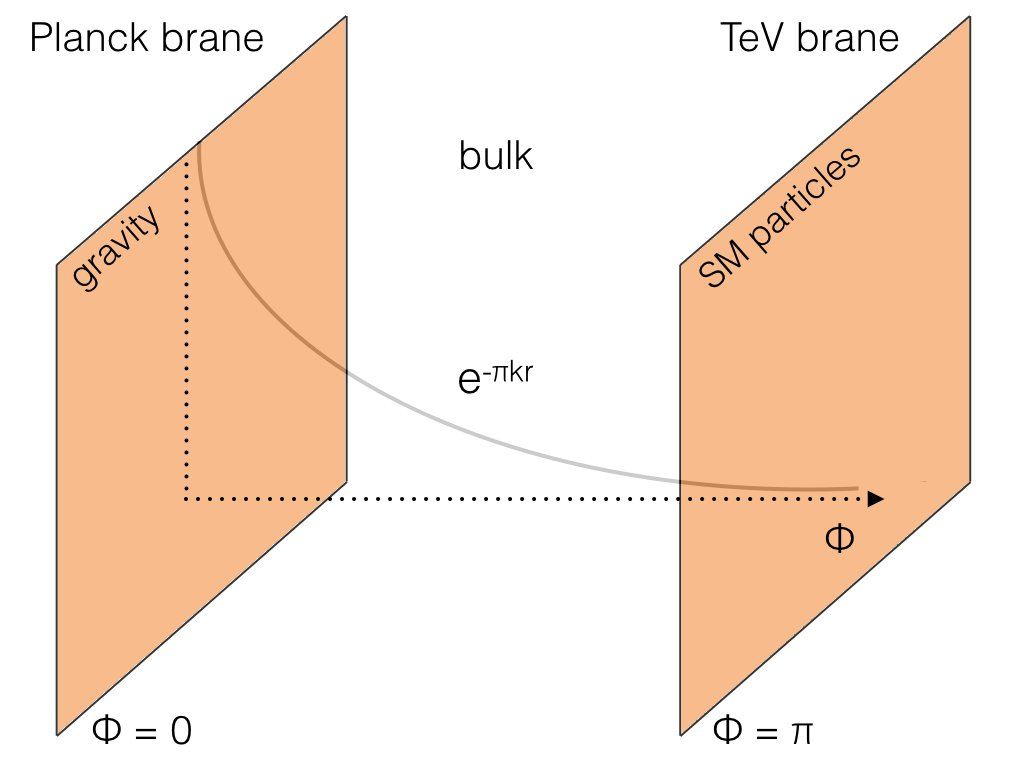
\includegraphics[width=0.35\textwidth]{\chtwo/RS1model.png}
 \caption{Set-up of the five dimensions in the RS model. The \textit{Planck} and \textit{TeV} branes are the 4-dimensional boundaries of the extra dimension $\phi$ compactified in an interval $[0,\pi]$.}
 \label{fig:WED}
\end{wrapfigure}

The basic RS model, referred to as RS1, assumes the existence of only one extra dimension with size $r_c$. This fifth, extra dimension is labelled by the coordinate $\phi \in [-\pi,\pi]$,
such that it can be described by a line segment between two 4-dimensional branes (or 3-branes), known as the \textit{Planck} and \textit{TeV} brane, located, respectively,
at the $\phi = 0$ and $\phi = \pi$ boundary of the fifth dimension (Fig.~\ref{fig:WED}).
In the simplest version of the RS model, it is assumed, like in the ADD case, that the SM fields live on the \textit{TeV} brane, while gravity lives everywhere.
The \textit{Planck} brane is where gravity is a relatively strong force.
The classical action describing the above set-up is given by the sum of the gravitational action in the bulk, $\mathcal{S}_{gravity}$, and on the two branes, $\mathcal{S}_{TeV}$ and $\mathcal{S}_{Planck}$,

\begin{equation}\label{eqn:WED_2}
\begin{gathered}
\mathcal{S} = \mathcal{S}_{gravity} + \mathcal{S}_{TeV} + \mathcal{S}_{Planck}, \\
\mathcal{S}_{gravity} = \int d^4x \int_{-\pi}^{+\pi} d\phi\sqrt{-G}{-\Lambda+2M^3_*R}, \\
\mathcal{S}_{TeV} = \int d^4x\sqrt{-G(x^\mu,\phi=\pi)}\Lambda, \\
\mathcal{S}_{Planck} = \int d^4x\sqrt{-G(x^\mu,\phi=0)}\Lambda.
\end{gathered}
\end{equation}

In the above equation, $G$ is the 5-dimensional metric $G_{\mu\nu}$, $\Lambda$ a cosmological constant, and $R$ the 5-dimensional Ricci tensor.
By requiring a solution of the 5-dimensional Einstein's equation for the above action that respects the 4-dimensional Poincar\'{e} invariance in the $x^\mu$ coordinates,
one finds that the 5-dimensional metric must take the form 

\begin{equation}\label{eqn:WED_3}
ds^2 = e^{-2\sigma(\phi)} \eta_{\mu\nu}dx^\mu dx^\nu + r^2_cd\phi,
\end{equation}

\noindent where $\eta_{\mu\nu} = \mathrm{diag}(1,-1,-1,-1)$ is the usual Minkowski metric and $\sigma(\phi)$ is some a priori unknown function.
This type of geometry is called ``non-factorizable'', because the metric of the 4-dimensional subspace is $\phi$-dependent.
Solving the 5-dimensional Einstein's equations provides a unique solution for $\sigma(\phi)$:

\begin{equation}\label{eqn:WED_4}
\sigma(\phi) = \sqrt{\frac{-\Lambda}{24M^3_*}} \equiv r_c|\phi|k,
\end{equation}

\noindent where $k$ is referred to as the \textit{curvature factor}.
By plugging the solution back into the original action and integrating out the extra dimension $\phi$, one finds that the 4-dimensional Planck mass is given by

\begin{equation}\label{eqn:WED_5}
\bMPl = \frac{M^3_*}{k}(1 - e^{-2\pi kr_c}).
\end{equation}

%\noindent where the term $e^{-2\pi kr_c}$ is usually called the \textit{warp factor}.
It is assumed that $k \sim M_* \sim \bMPl$ in order to avoid producing strong hierarchy between the mass scales of the theory.
However, the electroweak energy scale $v$ or any physical mass $m$ in the \textit{TeV} brane is exponentially suppressed compared to the 5-dimensional energy $v_0$ or mass $m_0$:

\begin{equation}\label{eqn:WED_6}
m = e^{-\pi kr_c}m_0 \, , \qquad\qquad v = e^{-\pi kr_c}v_0.
\end{equation}

This means that by taking $v_0$ of the order of the 5-dimensional fundamental mass scale $M_*$, the separation between the Planck mass and electroweak scales
is produced by the metric when $kr_c \sim 11$ (small hierarchy). Such factor indeed would already suppress a parameter with value of order $10^{18}\GeV$ to only 1\TeV.
The hierarchy is thus naturally established by the warp factor $e^{-\pi kr_c}$.
This Planck-electroweak hierarchy explanation is the most celebrated achievement of WED scenarios.

A distinctive novel feature of the RS scenario is the existence of a so-called tower of Kaluza--Klein (KK) excitations of a spin-2 field, the KK graviton, arising from tensor fluctuations 
around the 4-dimensional part of the metric. Scalar fluctuations around the fifth extra dimension give rise to a spin-0 field called \textit{radion}.
Massive graviton excitations appear, with 4-dimensional effective masses given by

\begin{equation}\label{eqn:WED_7}
m_G^{(n)} = kx_ne^{-\pi kr_c},
\end{equation}

\noindent where $x_n$ is the $n$-th root of the Bessel function $J_1$. These masses are of order of a TeV, so that Kaluza-Klein gravitons can be detected as massive resonances in collider experiments. 
The zero-mode of the graviton field corresponds to the mediator of gravitational interaction, and its wave function is highly peaked at $\phi = 0$. Gravity is thus localized on the \textit{Planck} brane, while on the \textit{TeV} brane we feel only the tail of the graviton wave-function. %So in the RS model the reason of the weakness of gravity is that it is localized far away from where we live.

The coupling of an excited graviton to matter is described by the Lagrangian

\begin{equation}\label{eqn:WED_8}
\mathcal{L} = - \frac{1}{\Lambda_\pi}T^{\mu\nu}\sum_{n>0}h^{(n)}_{\mu\nu},
\end{equation}

\noindent where $T^{\mu\nu}$ is the energy-momentum tensor of the matter field, $h^{(n)}_{\mu\nu}$ is the $n$-th excitation of the graviton,
and $\Lambda_\pi = \bMPl e^{-\pi kr_c}$ is of order of TeV.
It is interesting to note that this model has only two free parameters: the mass of the first (lightest) KK-graviton excitation, $m_1$, and the ratio $\tilde{k} \equiv  k/\bMPl$, which controls the widths of the new resonances:

\begin{equation}\label{eqn:WED_9}
\Gamma_n = \rho m_n x^2_n\tilde{k}^2,
\end{equation}

\noindent where $\rho$ is a constant depending on the number of open decay channels.
The RS model in its simplest form is thus highly predictive.\\

In the original RS1 model the SM matter is localized on the \textit{TeV} brane, as the Higgs field.
A well-motivated extension of the original RS1 model explored an alternative scenario, in which 
SM fields propagate in the warped bulk, except for the Higgs field which is required on the \textit{TeV} brane to avoid hierarchy.
This extension is referred thereafter as the \textit{bulk scenario}~\cite{Agashe:2007zd,Fitzpatrick:2007qr}.
Similarly to the KK-graviton excitations, in the bulk scenario a KK expansion is applied to each SM field.
The zero-mode of each KK tower represents the correspondent SM particle.
The first and second generation fermions are localized near the \textit{Planck} brane, leading to the the small Yukawa couplings to the Higgs field which is localized on the \textit{TeV} brane.
Similarly, the top quark can be localized near the \textit{TeV} brane to account for its large Yukawa coupling.
In the original RS1 scenario all the particles are localized on the \textit{TeV} brane, therefore the strength of the couplings between KK-graviton and SM particles are democratic. 
As a consequence, the RS gravitons are produced via both \qqbar annihilation and gluon fusion processes.
In the bulk scenario, couplings of KK gravitons to light fermions are highly suppressed since, as mentioned above, KK gravitons are localized near the \textit{TeV} brane, whereas light fermions are localized near the \textit{Planck} brane. As a result, \qqbar annihilation at hadron collider for KK graviton production is negligible in this case.
In contrast, SM gluons have a flat localization in the bulk, so that the coupling of gluons to KK gravitons and hence KK graviton production via gluon fusion is dominant.
Furthermore, decays of KK graviton into top quarks and Higgs bosons are enhanced due to their profile being near the \textit{TeV} brane, resulting in couplings to KK gravitons (which are also localized there) being only $\sim\TeV$-suppressed just like in the original RS1 model (Eq.~\ref{eqn:WED_8}).
Another crucial point of the bulk scenario is that before symmetry-breaking, the \PW and \PZ gauge bosons start out with flat localization in the bulk. %and the Higgs starts out with a delta function wave-function on the brane.
However, after symmetry-breaking, the gauge bosons eat a Higgs, and their wave functions are still mostly flat in the bulk but fall sharply near the brane.
Thus, in the bulk scenario, branching fractions for decays into pair of vector bosons are the same size as those for decays into Higgs bosons or top quarks.
The branching fractions for the different decay modes of the graviton in both the bulk and RS1 scenarios are shown in Fig.~\ref{fig:GrBR} as a function of the graviton mass.
It can also be shown that in RS1 scenario the graviton decays preferentially to transverse polarized vector bosons, whereas in the bulk scenario it decays preferentially to longitudinally polarized modes, making those two benchmarks an excellent framework to study the sensitivity of the vector boson identification techniques used at the collider experiments to the polarization (Chapter~\ref{ch:vtagging}).

\begin{figure}[!htb]
\centering
\subfigure[]{\label{fig:GrBR_a}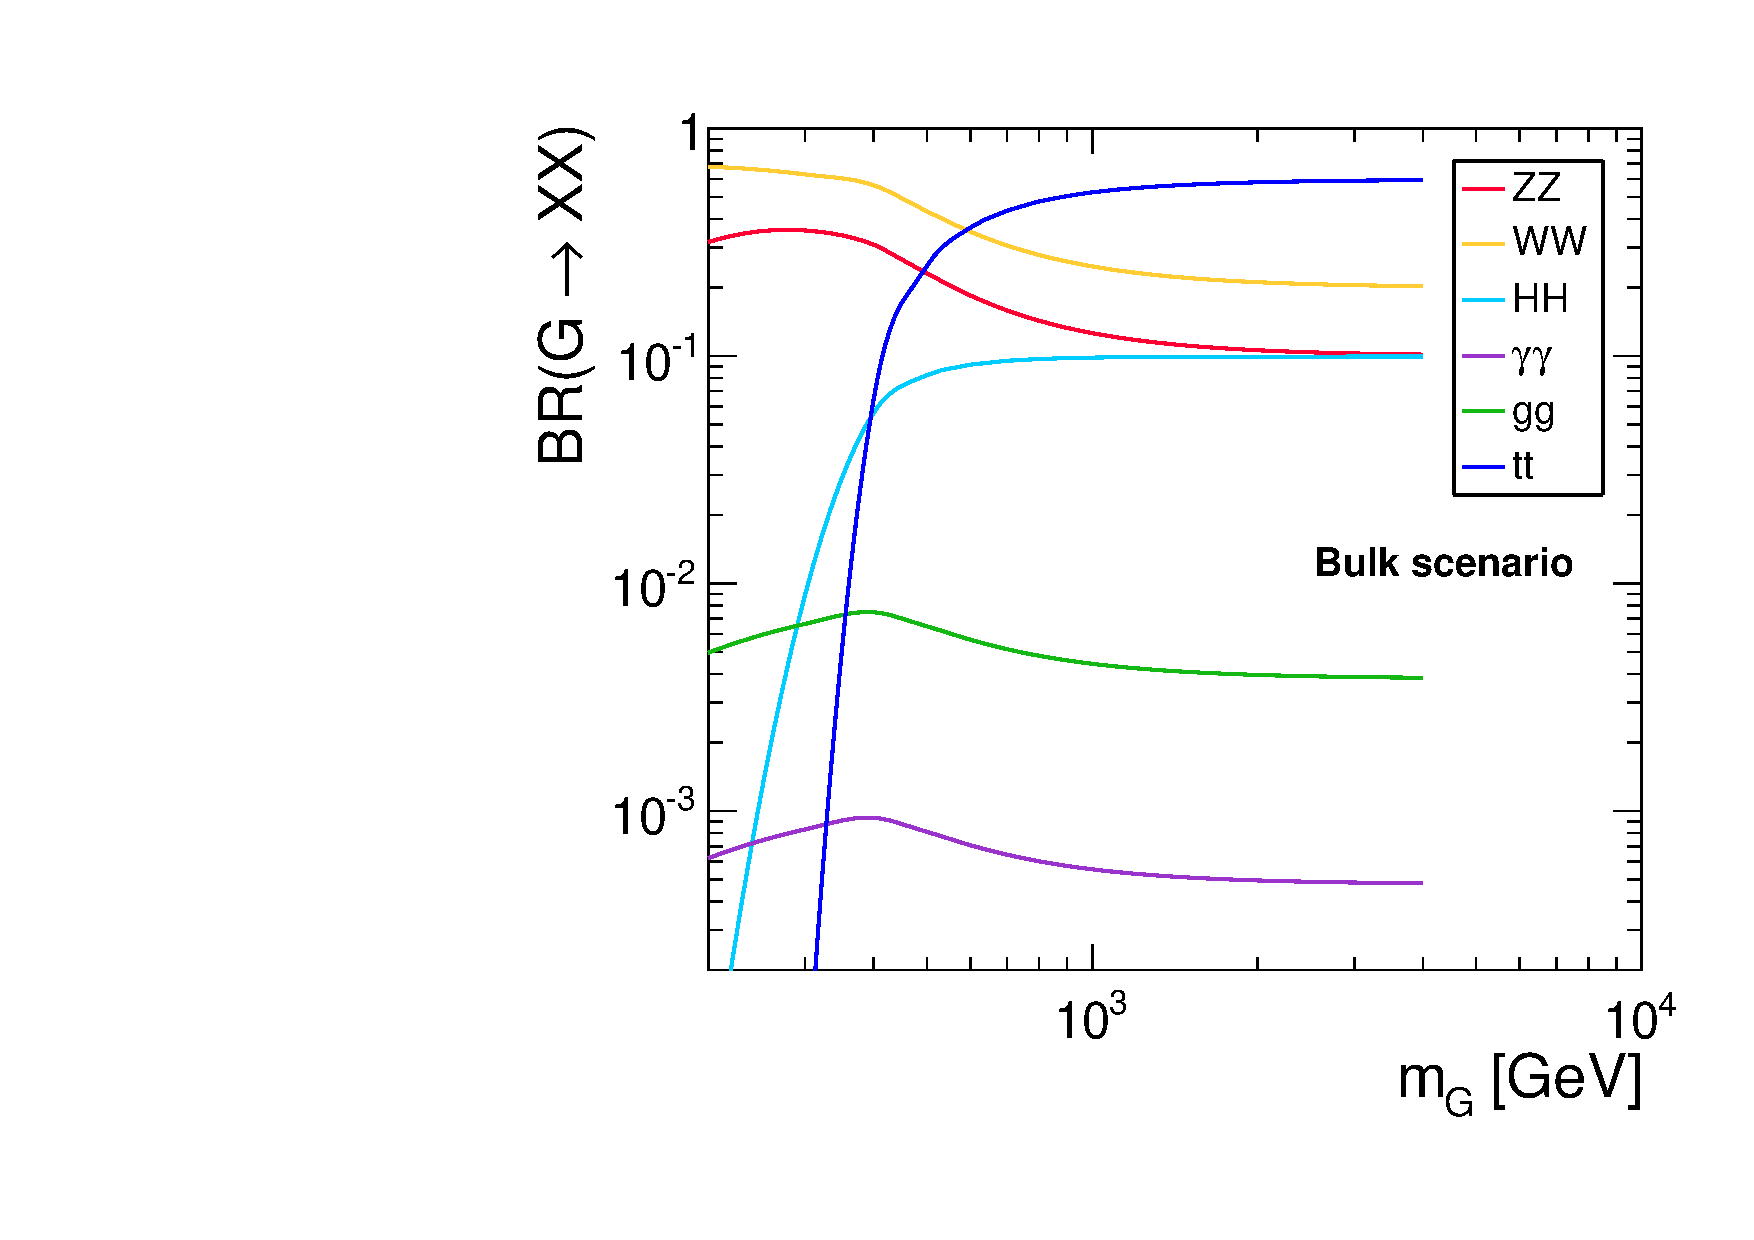
\includegraphics[width=0.45\textwidth]{\chtwo/brs-bulkg.pdf}}
\subfigure[]{\label{fig:GrBR_b}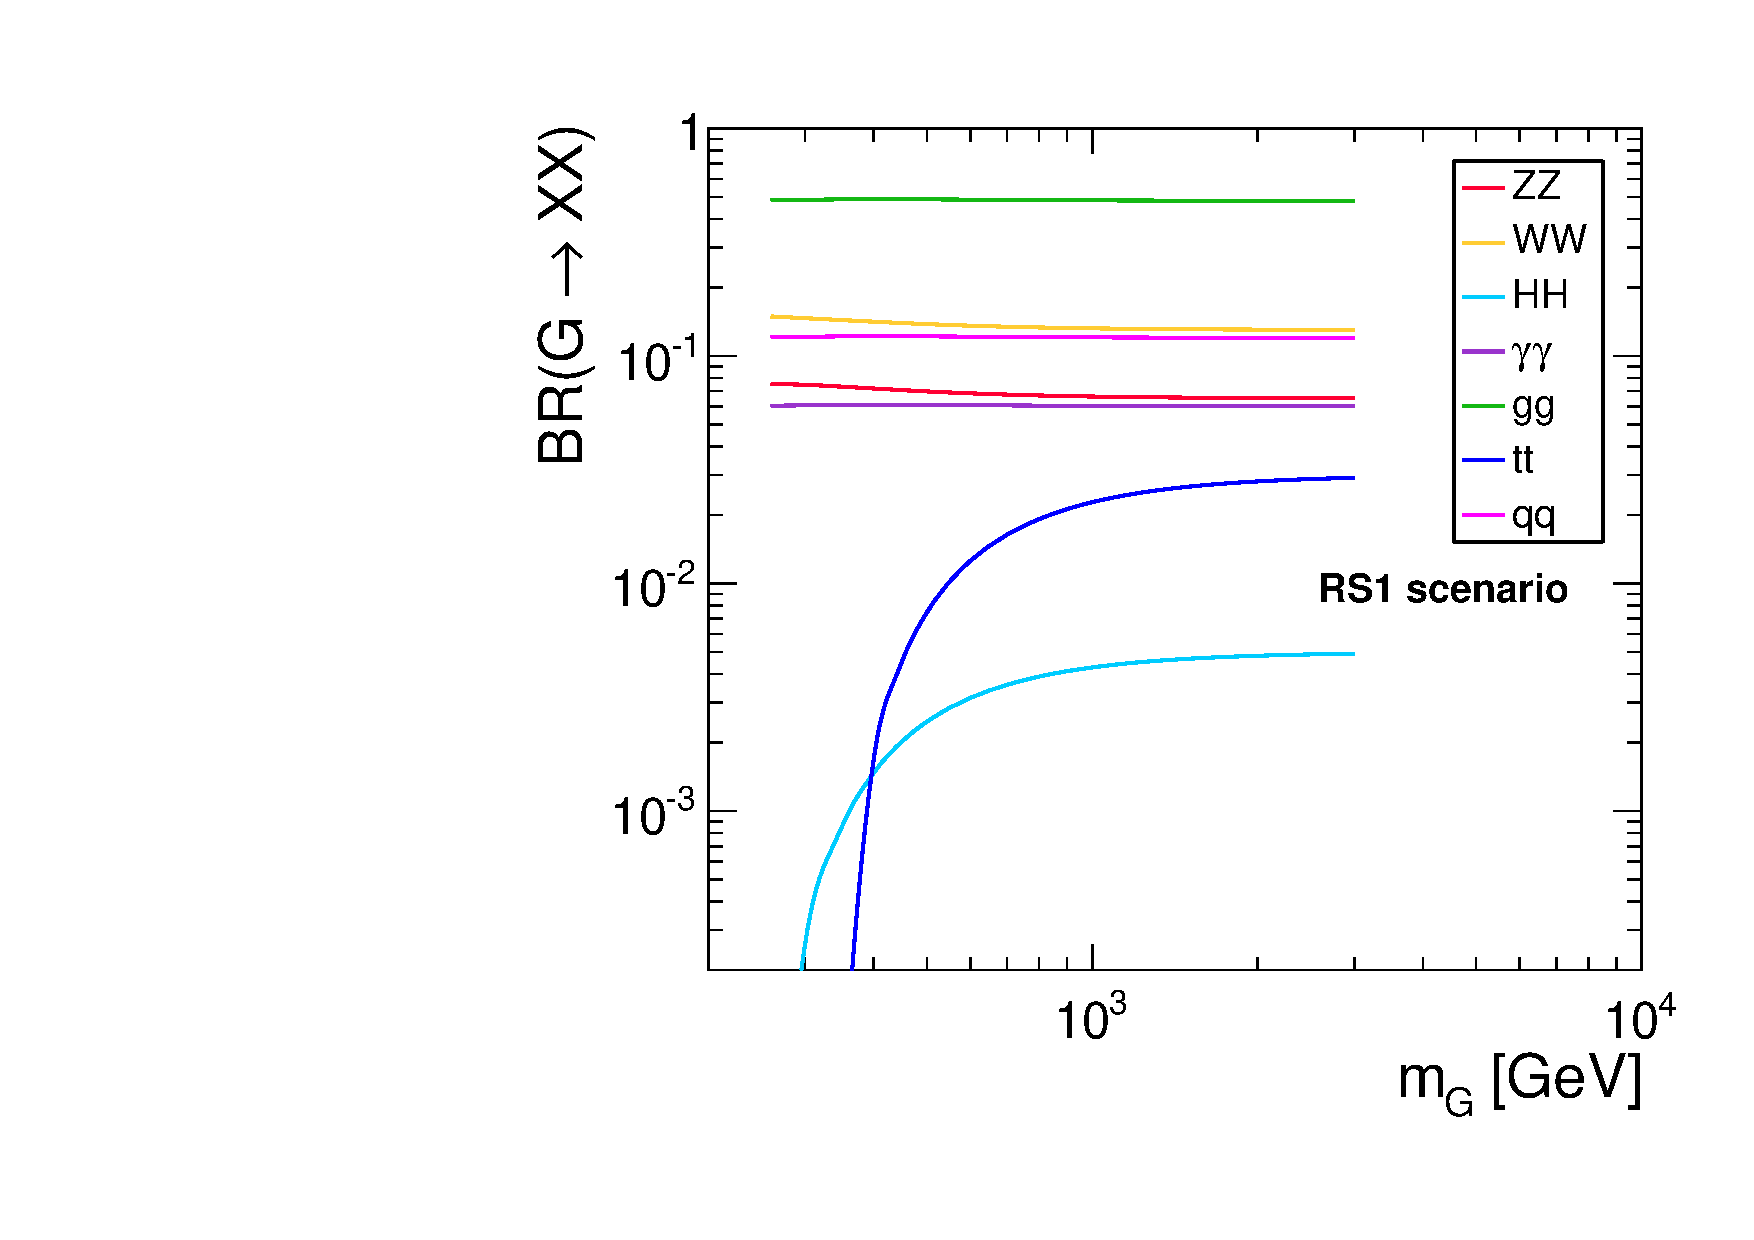
\includegraphics[width=0.45\textwidth]{\chtwo/brs-rs1.pdf}}
\caption{Branching fractions for the different decay modes of the graviton in the (a) bulk and (b) RS1 scenarios, as a function of the graviton mass.}
\label{fig:GrBR}
\end{figure}

%%%%%%%%%%%%%%%%%%%%%%%%%%%%%%%%%%%%%%%%%%%%
\subsection{Compositeness}\label{subsec:composite}
%%%%%%%%%%%%%%%%%%%%%%%%%%%%%%%%%%%%%%%%%%%%

One of the approaches to the hierarchy problem compatible with observations is based on the assumption that the Higgs boson is a composite particle, a bound state of more fundamental constituents held together by a new strong force.
In composite Higgs models~\cite{Composite0,Composite1,Composite2}, $\Lambda$ is the energy scale where the composite nature of the Higgs boson becomes important, which roughly coincides with the confinement scale of the new strong interaction. Thus, the solution to the hierarchy problem is that there is no elementary scalar, and beyond $\Lambda$ an experiment becomes sensitive to the underlying ``partons'' that compose the Higgs boson. 
However, precision electroweak data rule out new strong interactions at scales below about 10\TeV.
One key question is therefore the lightness of the Higgs boson with respect to such scale.

By comparing with the QCD sector, one observes that the strong coupling scale is $\Lambda_\mathrm{QCD} \sim \mathcal{O}(300\MeV)$, whereas most bound states, such as the $\rho$ meson and proton, are at least as heavy as this.
However, a counter-example in QCD is given by the existence of the pions, which are all lighter than $\Lambda_\mathrm{QCD}$, although only by a $\mathcal{O}(1)$ factor.
The reason for the pions to be appreciably lighter than the other QCD bound states is found in the chiral perturbation theory. 
In fact, the pions represent the Goldstone bosons of the spontaneously broken $SU(2)_L \times SU(2)_R$ flavor symmetry coming from chiral rotations of the up and down quarks. 
The spontaneous symmetry breaking of the flavor symmetry into the vectorial isospin subgroup $SU(2)_V$, is induced by a non-perturbative QCD vacuum state, characterized by a non-vanishing quark condensate $\langle \bar{q}^a_L q^b_R \rangle \sim \delta^{ab}\Lambda^3_\mathrm{QCD}$.
However, because of the non-vanishing and differing masses of the quarks, the $SU(2)_L \times SU(2)_R$ is only an approximate symmetry, and therefore the pions are not massless, but have small masses, so that they are \textit{pseudo-Goldstone bosons}.

In composite Higgs models, a similar structure is assumed, where the Higgs is a pseudo-Goldstone boson of some symmetry with strong coupling scale $\Lambda \approx 4\pi f$,
where $f$ is the scale at which the symmetry is spontaneously broken.
The main idea is that the Higgs mass parameter is protected against quadratic quantum corrections up to the compositeness scale because it is a pseudo-Goldstone boson. 
Above the scale of compositeness, it is simply not an elementary scalar.
Furthermore, the pseudo-Goldstone nature of the Higgs is an explanation for why the Higgs mass is so much lighter than the other bound states in the strongly coupled sector.

Such models start with a large global symmetry group $G$, analogous to the ``large'' $SU(2)_L \times SU(2)_R$ global symmetry of low energy QCD.
The strong dynamics spontaneously breaks $G$ to a subgroup $H$, similarly to the QCD chiral symmetry breaking $SU(2)_L \times SU(2)_R \to SU(2)_V$.
In a minimal composite Higgs model $G = SO(5) \to H = SO(4)$.
The SM electroweak group $SU(2)_L \times U(1)_Y$ is a subgroup of $H$, thus introducing a preferred orientation in the coset space SO(5)/SO(4) with respect to the global SO(4).
In this way, the electroweak scale $v$ is distinct from the $G \to H$ symmetry breaking scale $f$. The parameter $\xi = (v/f)^2$ is introduced to characterize this separation of scales and to quantify the degree of vacuum misalignment.
In a theory with little hierarchy $\xi \sim 1$, while a small amount of fine-tuning can give rise to $\xi \ll 1$. In particular, compatibility with the constraints coming from electroweak precision tests and Higgs coupling measurements generically implies $\xi \lesssim 0.2$. This bound places the scale $f$ at about 1\TeV, resulting in a strong coupling scale $\Lambda \approx 4\pi f \sim 10\TeV$.
Such large value results in a large one-loop contribution to the Higgs mass parameter (Eq.~\ref{eqn:HiggsCorr}), so that a generic composite Higgs set up still requires some tuning between the $v$ and $f$ scales.
One way to generate a ``little hierarchy'' is through the mechanism of \textit{collective symmetry breaking} as in \textit{Little Higgs} (LH) scenarios~\cite{Han:2003wu,Perelstein:2005ka,Schmaltz:2005ky,Arkani:2002LH}, which is now a key ingredient in composite Higgs models.
The main idea of this approach is that one can separate the scales $v$ and $f$ by introducing new particles, which cancel the quadratic divergences at one-loop order. 
In particular, the quadratic divergence induced by the SM gauge boson loops are canceled by the quadratic divergence induced by heavy gauge bosons at one loop level.
Heavy fermionic states are also introduced, which couple to the Higgs field such that the one-loop quadratic divergence induced by the top-quark Yukawa coupling to the Higgs boson is canceled.
Furthermore, extra Higgs fields exist as the Goldstone boson multiplets from the global symmetry breaking.
%In Little Higgs models, instead of a simple global group $G$ a direct product of two (or more) groups $G_1 \times G_2 \times \dotsc$ is considered so that its breaking has a collective nature.
%The models then contain additional gauge bosons at the TeV scale that produce the necessary cancellations to the one-loop quadratic divergence.
%It implies that any non-vanishing quantum contribution to the Higgs mass parameter must necessarily be proportional to a product of all the gauge coupling constants corresponding to the different $G_i$ factors.
%Thus, setting any one of the coupling constants to zero must result in a vanishing contribution.
%The extended gauge group $G_1 \times G_2 \times \dotsc$ of the LH models is typically broken down to the SM $\mathrm{SU(2)_L \times U(1)_Y}$ at a scale $f$ by the same condensates that break $G \to H$.
%The models then contain additional gauge bosons at the TeV scale. In the mass eigenbasis, the vanishing of the one-loop quadratic divergence can be understood as a result of a cancellation between the SM bow tie diagrams and their counterparts involving the TeV-scale bosons. 
This is achieved by enlarging the simple global group $G$ and embedding two parallel global symmetries $G_1 \times G_2$, such that $G \supset G_1 \times G_2 = [SU(2)_1 \times U(1)_1] \times[SU(2)_2 \times U(1)_2]$.
A specific implementation, called the \textit{littlest Higgs}~\cite{Arkani:2002LH}, starts with the global symmetry $G$ = SU(5), which is spontaneously broken down at the scale $\Lambda$ to its subgroup $SO(5)$ via a vacuum expectation value of order $f$. At the same time, the gauge symmetry $[SU(2) \times U(1)]^2$ is also broken into $[SU(2)_L \times U(1)_Y]$, identified as the SM gauge group.
The global symmetry breaking leaves 14 massless Goldstone bosons, which become the longitudinal components of the $\mathrm{W}^{\prime\pm}$  and $\PZpr$ gauge bosons associated with the broken gauge groups, giving them masses of the order $f$:

\begin{equation}\label{eqn:LHvprimeMass}
M(\mathrm{W}^{\prime\pm}) \simeq M(\PZpr) = \frac{g}{\sin2\theta}f,
\end{equation}

\noindent where $\theta$ is given by the gauge couplings of the two broken $SU(2)$ groups: $\tan\theta = g_1/g_2$.
The partial decay widths are computed using the formalism of Feynman rules:

\begin{equation}
\begin{aligned}
\Gamma(\mathrm{W}^{\prime\pm} \to \ell\nu) & \simeq \Gamma(\PZpr \to \ell\ell) & = \frac{g^2\cot^2\theta}{96\pi}M\\
\Gamma(\mathrm{W}^{\prime\pm} \to \mathrm{q}\bar{\mathrm{q}}^\prime) & \simeq \Gamma(\PZpr \to \qqbar) & = \frac{g^2\cot^2\theta}{32\pi}M\\
\Gamma(\mathrm{W}^{\prime\pm} \to \PW\PH) & \simeq \Gamma(\PZpr \to \PZ\PH) & = \frac{g^2\cot^22\theta}{192\pi}M\\
\Gamma(\mathrm{W}^{\prime\pm} \to \PW\PZ) & \simeq \Gamma(\PZpr \to \PW\PW) & = \frac{g^2\cot^22\theta}{192\pi}M
\end{aligned} 
\end{equation}

\noindent where $M$ is the mass of the \PVpr triplet given by Eq.~\ref{eqn:LHvprimeMass}.
Summing over all the quark and lepton channels results in a total width

\begin{equation}
\Gamma_\mathrm{tot} = \frac{g^2}{96\pi}(\cot^22\theta + 24\cot^2\theta)M.
\end{equation}

One can immediately observe that the fermionic decay modes dominate for $\cot\theta \geq 1/2$, while bosonic decay modes become significant only below this value.
However, since the \PVpr resonances are produced mainly via the Drell-Yan process $\qqbarpr \to \PVpr$, one should notice that the production cross section would be at the same time suppressed for the enhanced bosonic channels.
Thus, the interactions of the new predicted particles is described within these theories, and detailed predictions of their properties are made.
Furthermore, they provide distinct signatures that can be searched for at the hadron collider.

%%%%%%%%%%%%%%%%%%%%%%%%%%%%%%%%%%%%%%%%%%%%
\subsection{Heavy vector triplet}\label{subsec:hvt}
%%%%%%%%%%%%%%%%%%%%%%%%%%%%%%%%%%%%%%%%%%%%

New heavy spin-1 resonances are predicted by several extensions of the standard model, such as the Composite Higgs and Little Higgs models described in the previous section.
A model-independent strategy has been proposed in Ref.~\cite{Pappadopulo:2014qza} to study these resonances, based on a simplified phenomenological Lagrangian, which reproduces a large class of explicit models.
The main reason for introducing a simplified model is that the experimental searches for new resonances are typically not sensitive to all the details and the free parameters of the chosen benchmark model, but only to those parameters or combinations of parameters that control the mass of the resonance and the interactions involved in its production and decay. Therefore one can employ a simplified description of the new phenomena, where only the relevant couplings and mass parameters are retained. In turn, the experimental results expressed in terms of the phenomenological parameters can be easily translated into the free parameters of any explicit model by computing the phenomenological/explicit parameter relations.\\

In this approach, a new real vector in the $\mathrm{SU(2)_L}$ representation is introduced in addition to the SM fields, describing one charged and one neutral heavy spin-1 particle (heavy vector triplet or HVT) with the charge eigenstate fields given by

\begin{equation}\label{eqn:HVT_1}
V^\pm_\mu = \frac{V^1_\mu \mp iV^2_\mu}{\sqrt{2}} \, \qquad\qquad V^0_\mu = V^3_\mu.
\end{equation}

The dynamics of the new vector is described by a simple phenomenological Lagrangian

\begin{equation}\label{eqn:HVT_2}
\begin{split}
\mathcal{L}_V = & -\frac{1}{4}\mathcal{D}_{[\mu}V^a_{\nu]}\mathcal{D}^{[\mu}V^{\nu]a} + \frac{m^2_V}{2}V^a_\mu V^{\mu a}\\
 & + ig_Vc_HV^a_\mu H^\dag\tau^a\overleftrightarrow{\mathcal{D}}^\mu H + \frac{g^2}{g_V}c_FV^a_\mu J^{\mu a}_F\\
 & + \mbox{extra terms}
 %& + \frac{g_V}{2}c_{VVV}\epsilon_{abc}V^a_\mu V^b_\nu\mathcal{D}^{[\mu}V^{\nu]c} + g^2_Vc_{VVHH}V^a_\mu V^{\mu a} H^\dag H - \frac{g}{2}c_{VVW}\epsilon_{abc}W^{\mu\nu a}V^b_\mu V^c_\nu,
 \end{split}
\end{equation}

\noindent where $g$ denotes the gauge coupling.
The first line of the above equation contains the kinetic and mass terms for the field $V$, plus trilinear and quadrilinear interactions with the vector bosons from the covariant derivatives.
The second line contains direct interactions of $V$ with the Higgs current in the first term, and with the SM left-handed fermionic currents $J^{\mu a}_F$ in the second term.
The Higgs current term with coefficient $c_H$ leads to vertices involving the physical Higgs field and the three unphysical goldstone bosons.
Since the goldstone bosons represent the longitudinally polarized SM vector bosons \PW and \PZ, the parameter $c_H$ controls the interactions of $V$ with the SM vector bosons and with the Higgs boson, and in particular its decay modes into these electroweak particles.
Similarly, the parameter $c_F$ describes the direct interaction with fermions, which is responsible for both the resonance production via \qqbar annihilation and for its fermionic decays.
One observes that a universal coupling of the new field $V$ to fermions is assumed in Eq.~\ref{eqn:HVT_2} for simplicity, such that $c_F$ represents the couplings to leptons ($c_\ell$), light quarks ($c_q$) and the third quark family ($c_3$).
The third line of the equation contains new operators and free parameters, which however have a sub-leading effect on the phenomenology of interest for resonant searches, and
therefore to a first approximation they can be neglected.% and the phenomenology described entirely by the three parameters $c_H$, $c_F$, and the mass $m_V$ of the new states.

In the adopted simplified description, the free parameter $g_V$ represents the typical strength of $V$ interactions, while the dimensionless coefficient $c_H$ parametrizes the departure from the typical strength.
Such parametrization is found convenient because, although the coefficient $c_F$ is of order one in most of the explicit models, the parameter $c_H$ is of order one in the strongly-coupled scenario (e.g., Composite Higgs models) but can be reduced in a weakly coupled case (e.g., extensions of the SM gauge group~\cite{PhysRevD.22.727,Altarelli}). The coefficients are never larger than one in all cases, whereas the coupling $g_V$ can vary over a large range in different scenarios, from $g_V \sim g \sim 1$ in the typical weakly-coupled case up to $g_V \sim 4$ in the strong limit. Therefore, it is more convenient to factor it out of the parametrization, although it is not a fundamental parameter of the model. For the purpose of presenting experimental results, the combinations $g_Vc_H$ and $g^2c_F/g_V$ that enter in the vertices are instead treated as fundamental parameters, as they control production and decay rates.

After electroweak symmetry breaking the heavy vector acquires mass and one finds that the charged and neutral $V$'s are practically degenerate ($M_\pm \simeq M_0 \simeq M_V$),
and therefore they are expected to have comparable production and decay rates at the hadron collider. The partial widths are as well immediately computed in this framework:

\begin{eqnarray}\label{eqn:HVT_3}
\Gamma_{V^\pm \rightarrow f\bar{f}^\prime} \simeq 2\Gamma_{V^0 \rightarrow f\bar{f}} & \simeq N_c[f] \left( \frac{g^2c_F}{g_V} \right)^2\frac{M_V}{48\pi}\nonumber \\
\Gamma_{V^\pm \rightarrow \PW\PZ} \simeq \Gamma_{V^0 \rightarrow \PW\PW} & \simeq \frac{g^2_Vc^2_HM_V}{192\pi}\\
\Gamma_{V^\pm \rightarrow \PW\PH} \simeq \Gamma_{V^0 \rightarrow \PZ\PH} & \simeq \frac{g^2_Vc^2_HM_V}{192\pi}\, , \nonumber
\end{eqnarray}

\noindent where $N_c[f]$ is the number of colors and is equal to three for the diquark and to 1 for the dilepton decays.
It can be observe that through the partial width to qq, the parameter $c_F = c_q$ controls the Drell-Yan production rate.
The channels which are not reported in Eq.~\ref{eqn:HVT_3} are either forbidden, like $\PH\PH$ and $\gamma\gamma$ decays, or suppressed like the decays to transverse polarizations or to $\PW\gamma$.

Two exemplary benchmark models, called A and B, are studied in Ref.~\cite{Pappadopulo:2014qza}, which correspond to two explicit models describing heavy vectors, namely those in Refs.~\cite{PhysRevD.22.727} and~\cite{Composite1}, respectively. The $c_F$ and $c_H$ coefficients are fixed to specific values in these models, and the only free parameters are the resonance coupling $g_V$ and its mass $M_V$.
Moreover, since models A and B are inspired, respectively, by weakly coupled extensions of the SM gauge group and strongly coupled scenarios, i.e. Composite Higgs models, the two benchmark models are considered in different regions of $g_V$, relatively small, $g_V \lesssim 3$, and relatively large, $g_V \gtrsim 3$, respectively. In particular, the branching fractions for the different decay modes of the neutral spin-1 resonance in models $\mathrm{A}_{g_V=1}$ and $\mathrm{B}_{g_V=3}$ are shown in Fig.~\ref{fig:hvtBR} as a function of the resonance mass. For these values of $g_V$, model A predicts comparable branching fractions for decay modes into fermions and bosons, as expected from Eq.~\ref{eqn:HVT_3}. In model B, on the contrary, $c_H$ is unsuppressed, and therefore the dominant branching fractions are into dibosons, whereas the fermionic decays are extremely suppressed.

\begin{figure}[!htb]
\centering
\subfigure[]{\label{fig:hvtBR_a}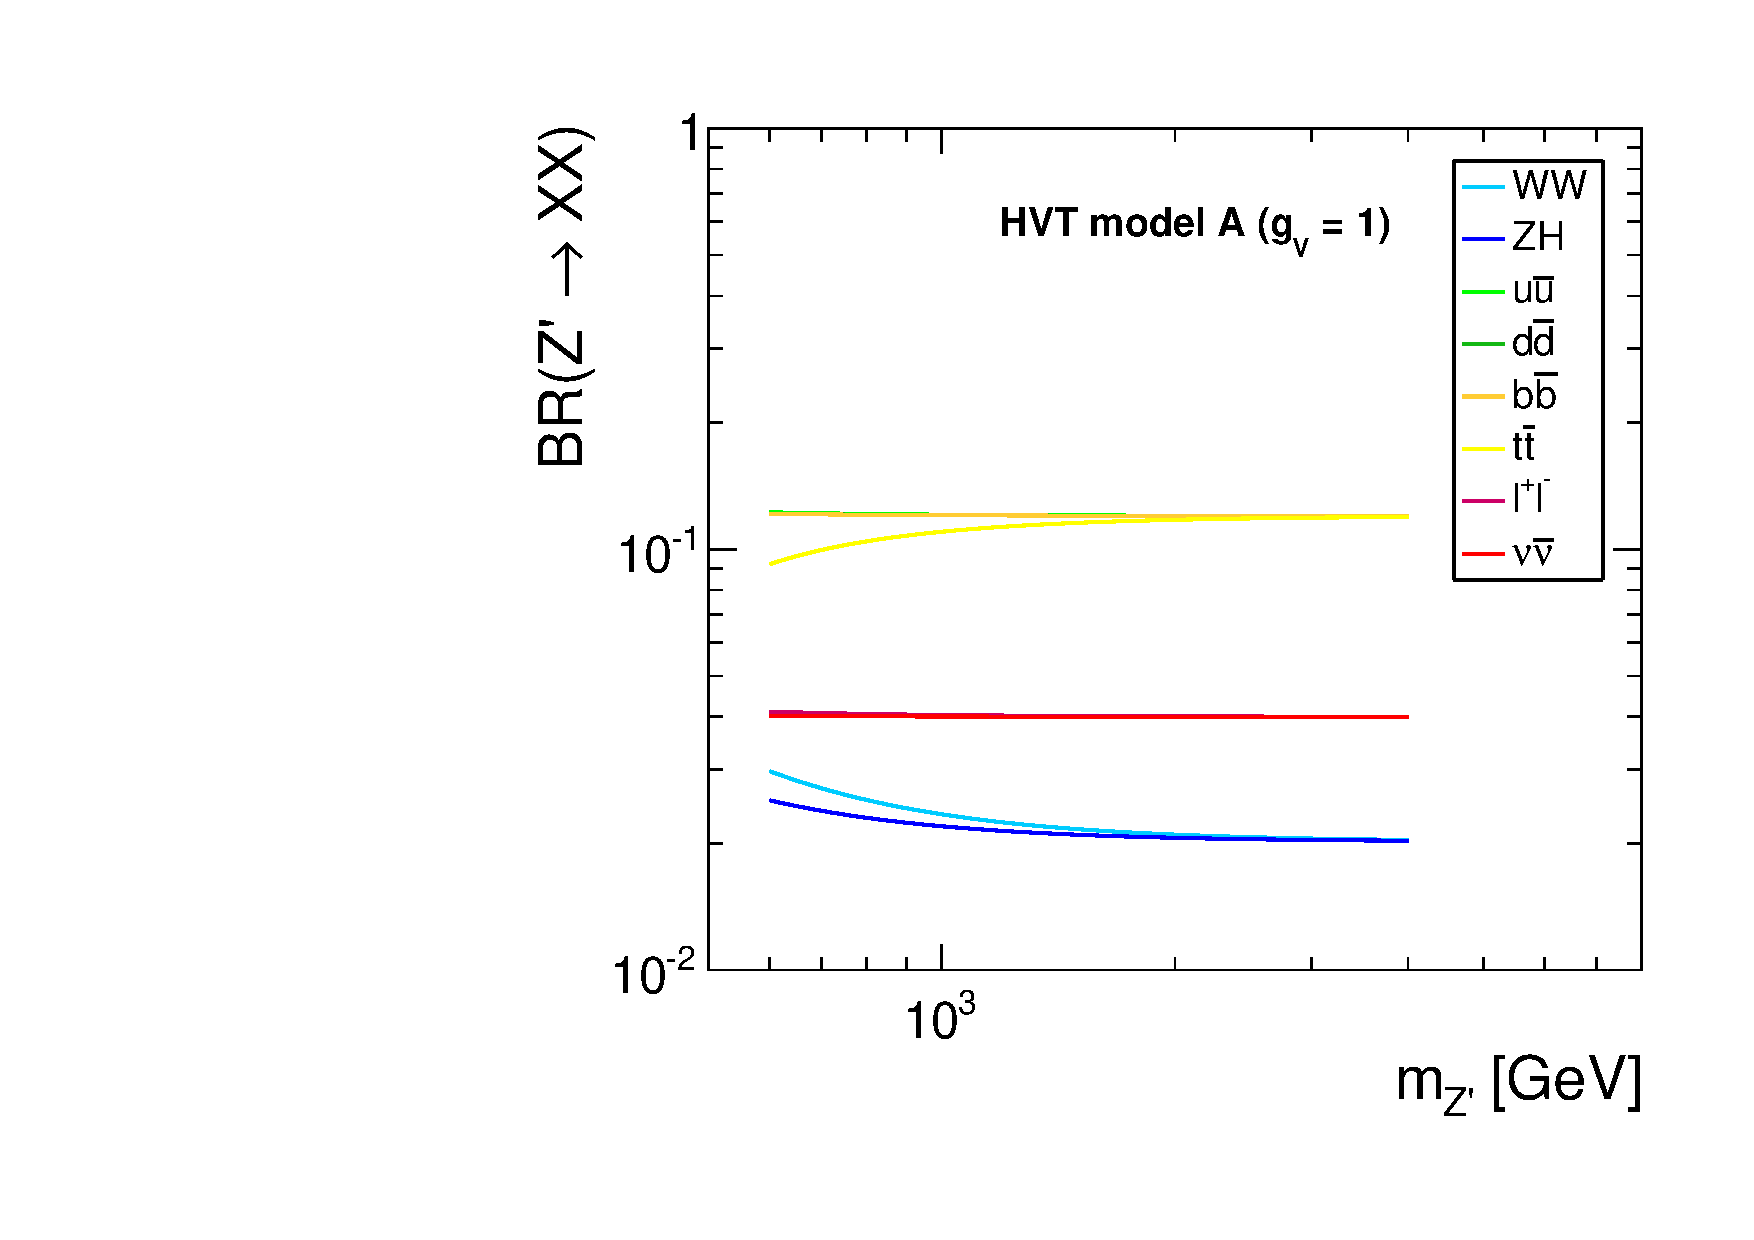
\includegraphics[width=0.45\textwidth]{\chtwo/brs-hvt-zprime-modelA.pdf}}
\subfigure[]{\label{fig:hvtBR_b}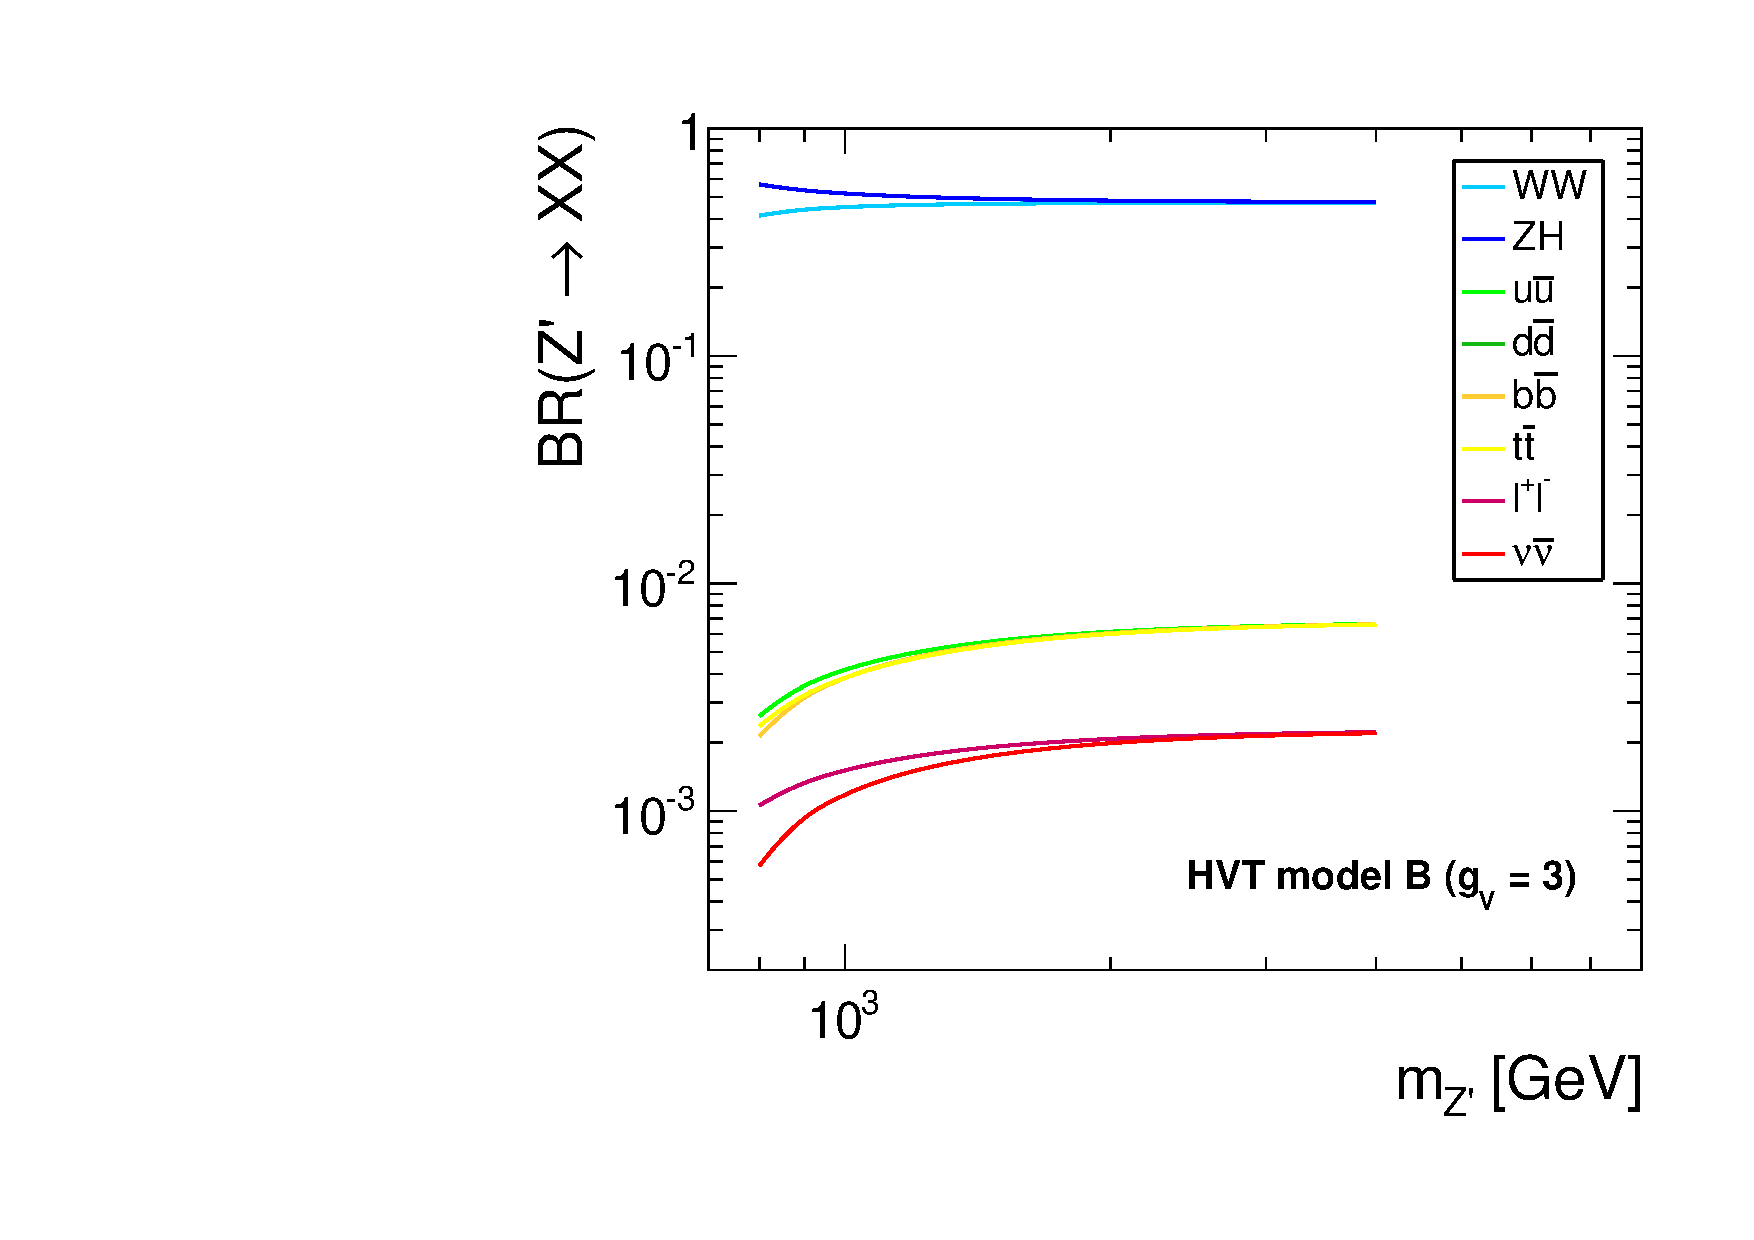
\includegraphics[width=0.45\textwidth]{\chtwo/brs-hvt-zprime-modelB.pdf}}
\caption{Branching fractions for the different decay modes of the neutral spin-1 resonance \Zpr ($V^0$) for the benchmarks (a) $\mathrm{A}_{g_V=1}$ (a) and (b) $\mathrm{B}_{g_V=3}$, as a function of the resonance mass.}
\label{fig:hvtBR}
\end{figure}

It has to be noted that the prediction of this simplified model are only valid for sufficiently narrow resonances.
In fact, several effects due to new physics, not included in this simplified framework, might contribute to the tail and radically change its prediction.
As a consequence, the results of an experimental search which is sensitive to the tail cannot be easily translated into bounds on the phenomenological parameter space.
  

		
%\chapter{The CMS Experiment at LHC} %add observational evidence
	\chapter{The CMS experiment at the LHC}
\label{ch:CMS}

%\section{The Large Hadron Collider}
    %//////////////////////////////////////////////////////////////////////////////////////////////////////////////////////////////////////////////////////

\section{The Large Hadron Collider}
\label{sec:LHC}

%//////////////////////////////////////////////////////////////////////////////////////////////////////////////////////////////////////////////////////

The Large Hadron Collider (LHC)~\cite{1748-0221-3-08-S08001} is a proton-proton (pp) collider located at the European Particle Physics Laboratory (CERN) near Geneva, Switzerland. It is situated in the former CERN Large Electron-Positron Collider (LEP) tunnel with a circumference of 27\unit{km} about 100\unit{m} under ground crossing the border between France and Switzerland. A hadron collider has been chosen to allow higher center-of-mass energies ($\sqrt{s}$) compared to electron-positron colliders, the latter limited by synchrotron radiation due to the low mass of the particles to be accelerated. High center-of-mass energies are required for the production of heavy SM particles such as the top quark and the Higgs boson, and to search for new BSM interactions at the TeV scale.
%heavy BSM resonances such as \cPZpr, \cPWpr or gravitons.
For this purpose, the LHC is designed to produce pp collisions up to a $\sqrt{s} = 14\TeV$, superseding previous high energy hadron colliders, such as Tevatron, by a factor of 7.
Higher center-of-mass energies lead to larger cross sections for the production of the physics processes of interest in parton-parton interactions (Fig.~\ref{fig:partonLumiRatio}), maximizing the sensitivity to new discoveries.
In addition to colliding protons, the LHC is also capable of accelerating and colliding heavy nuclei, which is, however, not considered in this work.

\begin{figure}[!htb]
 \begin{center}
  %\subfigure[]{\label{fig:partonLumiRatio_a}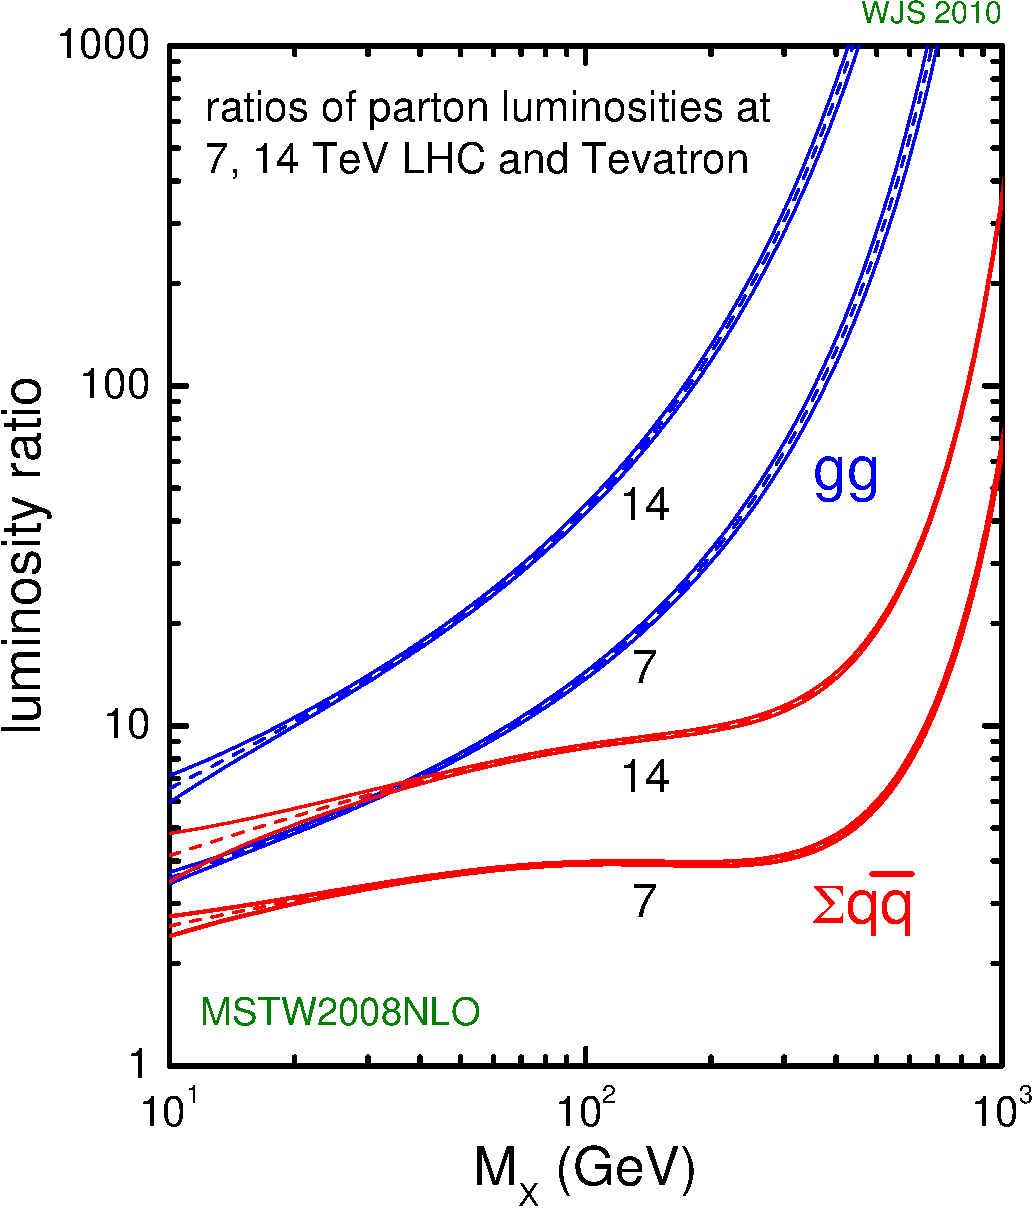
\includegraphics[width=0.25\textwidth]{\chthree/lumiTevLHC714.pdf}}
  %\subfigure[]{\label{fig:partonLumiRatio_b}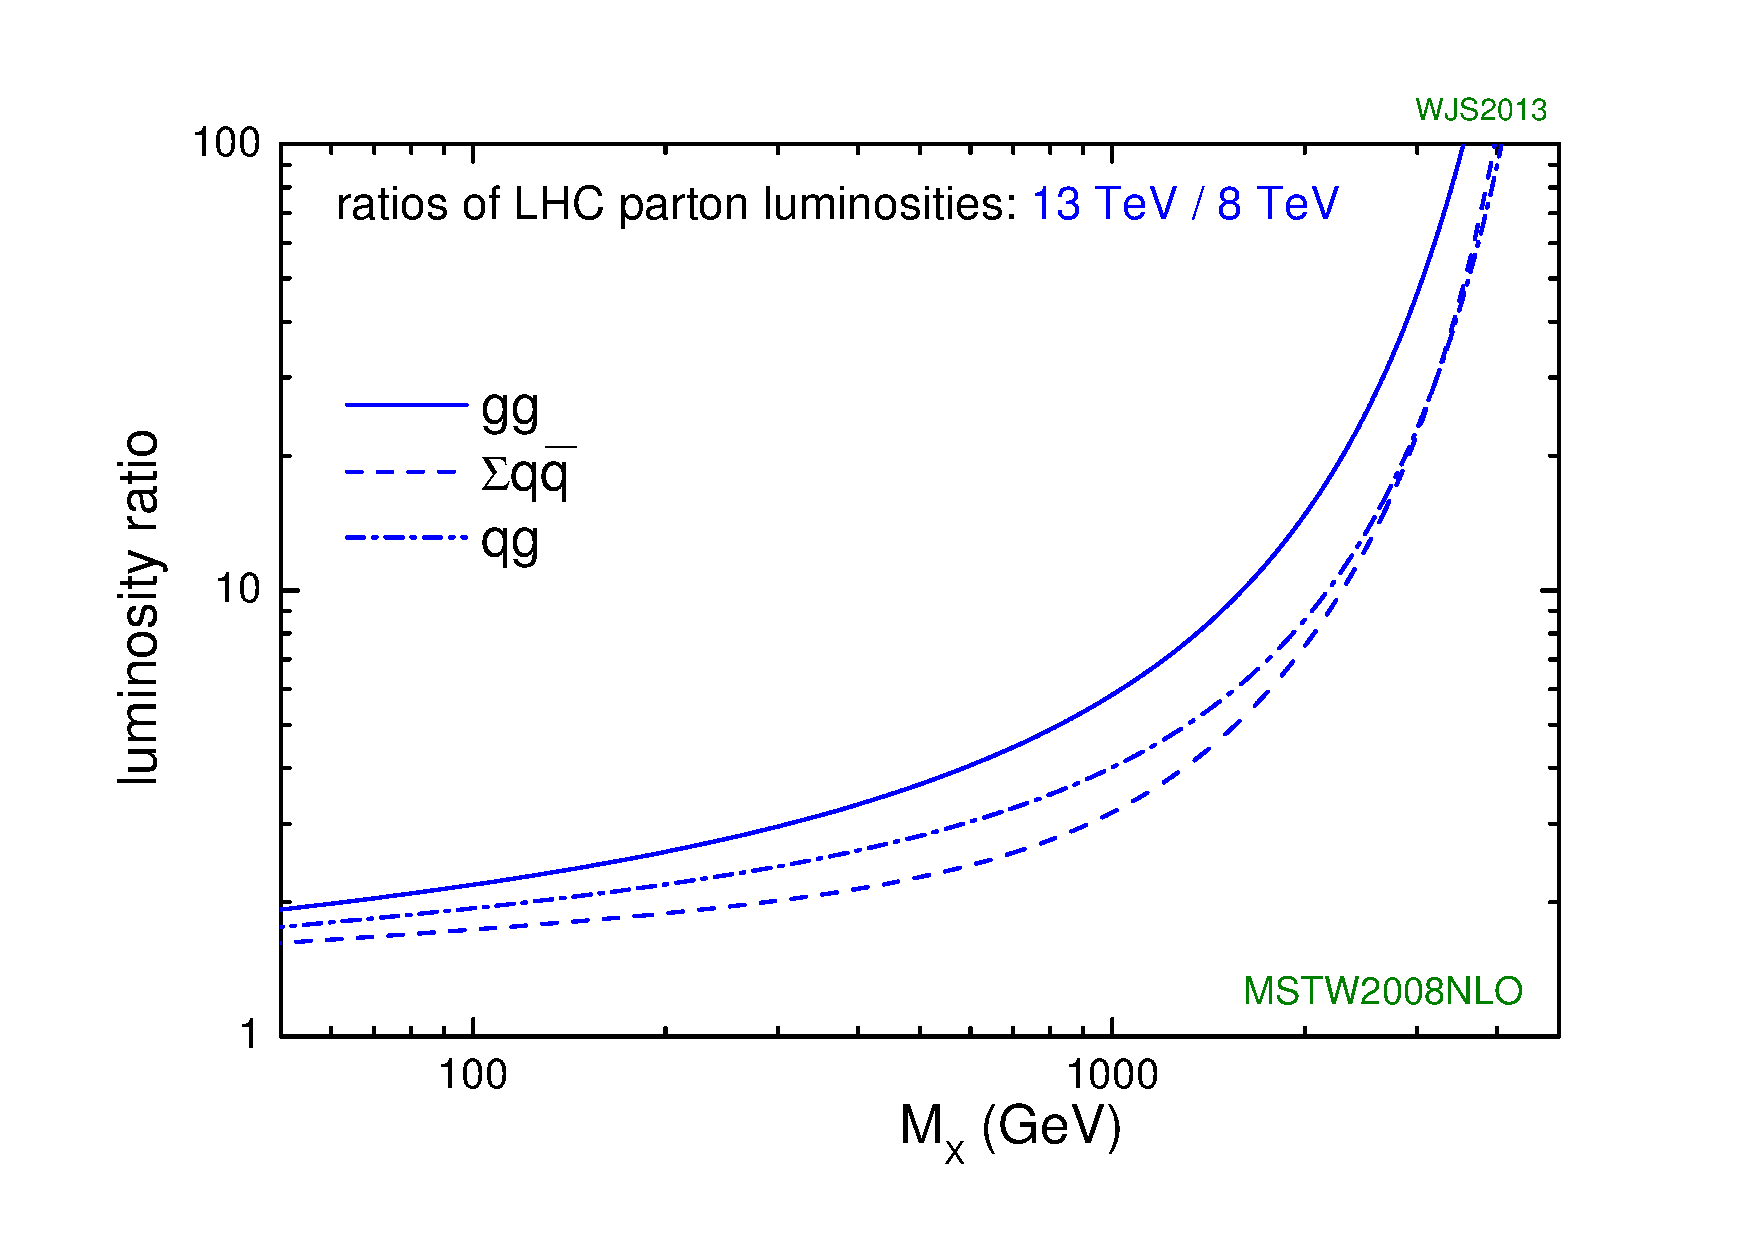
\includegraphics[width=0.46\textwidth]{\chthree/lhclumi7813_2013_v1.pdf}}
  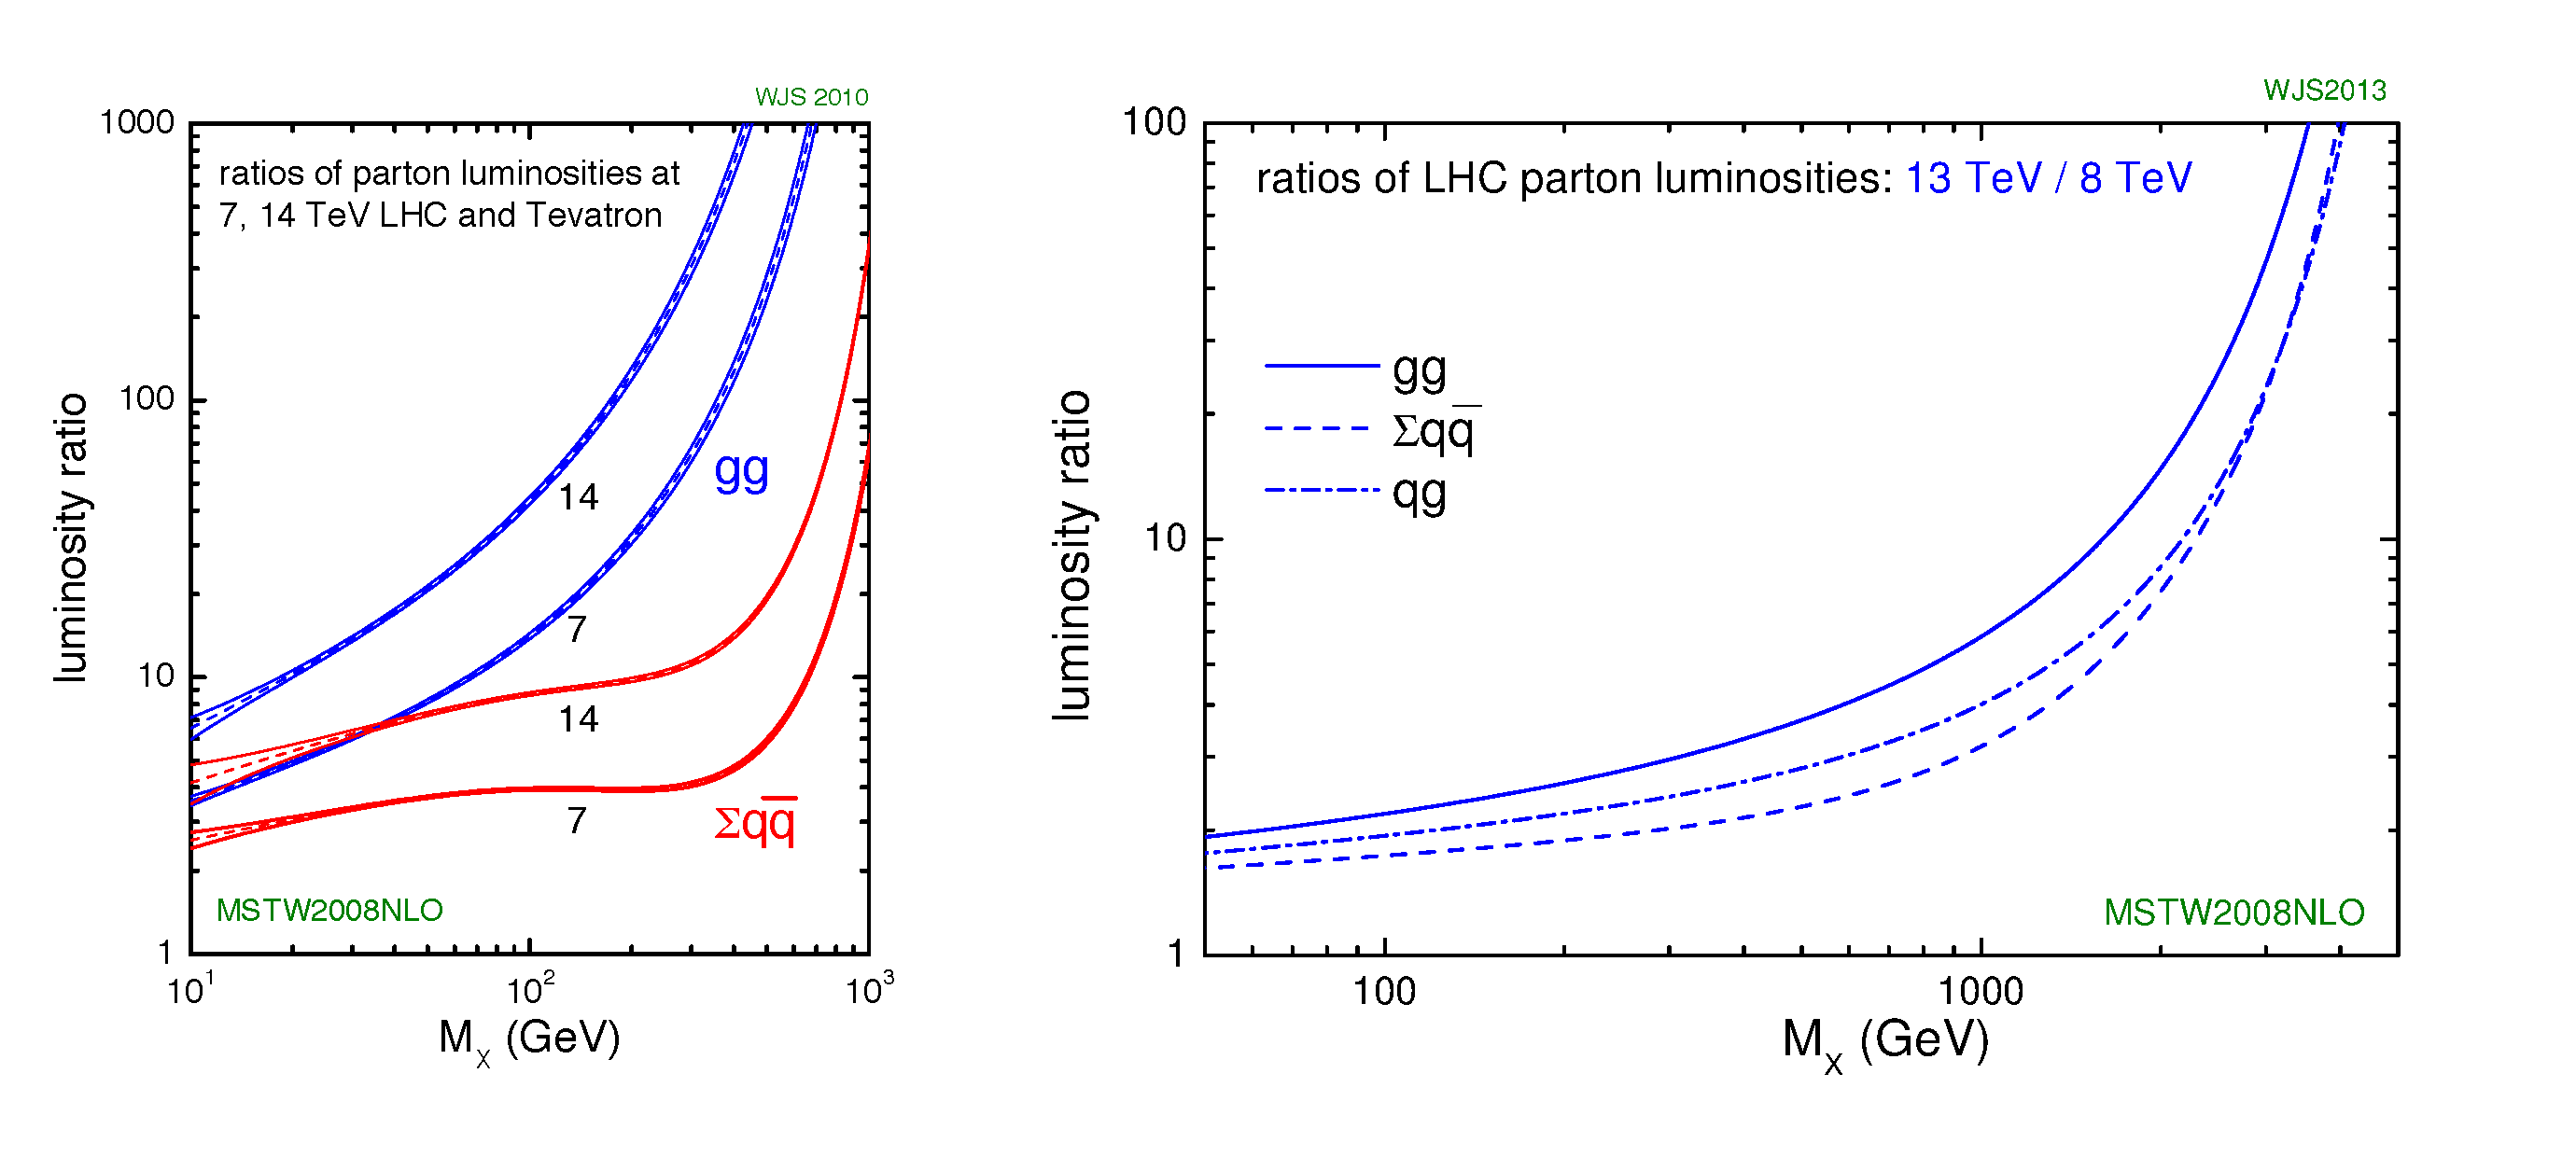
\includegraphics[width=\textwidth]{\chthree/lumiratios.pdf}
 \end{center}
 \caption{(left) Parton luminosity ratios of pp collisions at LHC at $\sqrt{s} = 7, 14\TeV$ and p$\bar{\mathrm{p}}$ collisions at Tevatron at $\sqrt{s} = 1.96\TeV$. (right) Parton luminosity ratios of pp collisions at LHC at $\sqrt{s} = 13\TeV$ and at $\sqrt{s} = 8\TeV$~\cite{LumiRatios}.}
 \label{fig:partonLumiRatio}
\end{figure}

The LHC is the final element in a succession of machines that accelerate protons to increasingly higher energies. 
%Each machine boosts the energy of a beam of protons, before injecting the beam into the next machine in the sequence. 
Protons, obtained from a hydrogen source, are first accelerated by a linear accelerator (LINAC 2) to energies of 50\MeV.
The beam is then injected into the Proton Synchrotron Booster (PSB), which accelerates the protons to 1.4\GeV, followed by the Proton Synchrotron (PS), which pushes the beam to 25\GeV. Protons are then sent to the Super Proton Synchrotron (SPS) where they are accelerated to 450\GeV.
%Using two transfer lines the protons are then injected into the two beam pipes of the LHC ring, where they circulate in opposite directions and accelerated up to the targeted energy. The LHC ring and the acceleration chain are sketched in Fig.~\ref{fig:LHC}.
Finally, the beam is injected in the LHC ring, where it completes several revolutions to reach the targeted energy. The LHC ring and the acceleration chain are sketched in Fig.~\ref{fig:LHC}.

Inside the ring, the two proton beams circulate in opposite directions in two tubes kept at ultrahigh vacuum, referred as beam pipes. The acceleration of protons inside LHC is made by radio-frequency cavities (400\unit{MHz}), giving a 492\keV energy gain per revolution, with a 7\keV loss per turn due to synchrotron radiation. It takes 4 minutes and 20 seconds to fill each LHC ring, and 20 minutes for the protons to reach their maximum energy of 7\TeV. The maximum energy of the protons is limited by the strength of the magnetic field required for keeping the protons inside the ring. For 7\TeV-protons a magnetic field of 8.3\unit{T} has to be produced, which can only be reasonably obtained by superconducting magnets. The ring is equipped with 1232 dipole magnets for bending and 392 quadrupole magnets for focussing made of niobium-titanium (NbTi), which are cooled down to a temperature of 1.9\unit{K} with the help of super-fluid helium.
%Superconducting magnets of different varieties and sizes are used to direct the beams around the accelerator.
%Among these, dipole magnets are used to bend the particle beam and to keep it into the circular tunnel. 
%There are 1232 main dipoles each 15 metres long and weighing in at 35 tonnes, which operate in a bath of liquid helium at a temperature of 1.9 K, that can provide a maximum magnetic field of 8.4 T (11850 A current).
%Additional 392 quadrupole magnets, each 5–7 metres long, are used to keep the beams focused, in order to maximize the chances of interaction between the particles in the four intersection points, where the two beams cross and the particle detectors are located.
After acceleration the protons move through the ring in separate bunches of protons with a fixed spatial separation.

The LHC ring has four interaction points at which the two counter rotating beams are made to cross and located in the center of the four LHC experiments. %and the particle detectors are located.
Just prior to collision, particles from the incoming beams must be squeezed closer together in order to maximize the chances of interaction. For this purpose, a system of three quadrupole magnets, so-called inner triplet, is located at both sides of each interaction point, which squeeze the beams and lead them to collisions in the center of the detector. Inner triplets tighten the beam, making it 12.5 times narrower� from 0.2\mm down to 16\mum across.
%After colliding, the particle beams are separated again by dipole magnets. Other magnets minimize the spread of the particles from the collisions. When it is time to dispose of the particles, they are deflected from the LHC along a straight line towards the beam dump. A "dilution" magnet reduces the beam intensity by a factor of 100,000 before the beam collides with a block of concrete and graphite composite for its final stop.
%Insertion magnets are also responsible for beam cleaning, which ensures that stray particles do not come in contact with the LHC’s most sensitive components.

Besides the high center-of-mass energy required for the production of heavy particles, a high event rate has to be obtained to allow the discovery of processes with low production cross sections. The instantaneous luminosity \Lumi characterizes the interaction rate. For a process with a cross section $\sigma$, the interaction rate is given by

\begin{equation}
\frac{dN_{ev}}{dt} = \sigma\Lumi.
\end{equation}

The instantaneous luminosity depends only on the beam parameters and can be written for a Gaussian beam distribution as:

\begin{equation}
\Lumi = \frac{N_b^2n_bf_{\rm rev}\gamma_r}{4\pi\sigma_x\sigma_y}~\mathrm{,}
\end{equation}
where $N_b$ is the number of particles per bunch, $n_b$ the number of bunches per beam, $f_{\rm rev}$ the revolution frequency, $\gamma_r$ the relativistic gamma factor, while $\sigma_x$ and $\sigma_y$ characterize the widths of the transverse beam profiles in the horizontal and vertical direction, respectively. The number of interaction events in a period of running time of the collider can be derived as

\begin{equation}
N_{ev} = \sigma \int \Lumi dt = \sigma L~\mathrm{,}
\end{equation}
where $L$ is called the integrated luminosity. It is a measurement of the collected data size and it is usually expressed in inverse of cross section.

The LHC beams can reach very high luminosity with a high frequency bunch crossing and a high density of protons per bunch. In the ring, 2808 bunches of $1.15\ten{11}$ protons are circulated, with an average length of 7.5\cm, a width of about 16\mum and a bunch spacing of 25\unit{ns} (collision frequency of 40\unit{MHz}). This corresponds to the design instantaneous luminosity of $10^{34}$\percms for pp collisions, which supersedes by a factor of 100 the luminosity reached by previous hadron colliders.

Proton collisions take place in four points of the LHC tunnel where the four main experiments are located: ATLAS (\textit{A Toroidal LHC ApparatuS})~\cite{Aad:2008zzm}, CMS (\textit{Compact Muon Solenoid})~\cite{Chatrchyan:2008zzk}, LHCb (\textit{LHC beauty experiment})~\cite{Alves:2008zz} and ALICE (\textit{A Lead Ion Collider Experiment})~\cite{Aamodt:2008zz}. ATLAS and CMS are general purpose experiments, designed to get an extensive study of SM and BSM physics and to operate at the design luminosity. The LHCb experiment is instead optimized for bottom quark physics studies while the ALICE experiment is dedicated to the study of the lead-lead collisions at the design luminosity of $10^{27}$\percms.\\

\begin{figure}[!htb]
 \begin{center}
  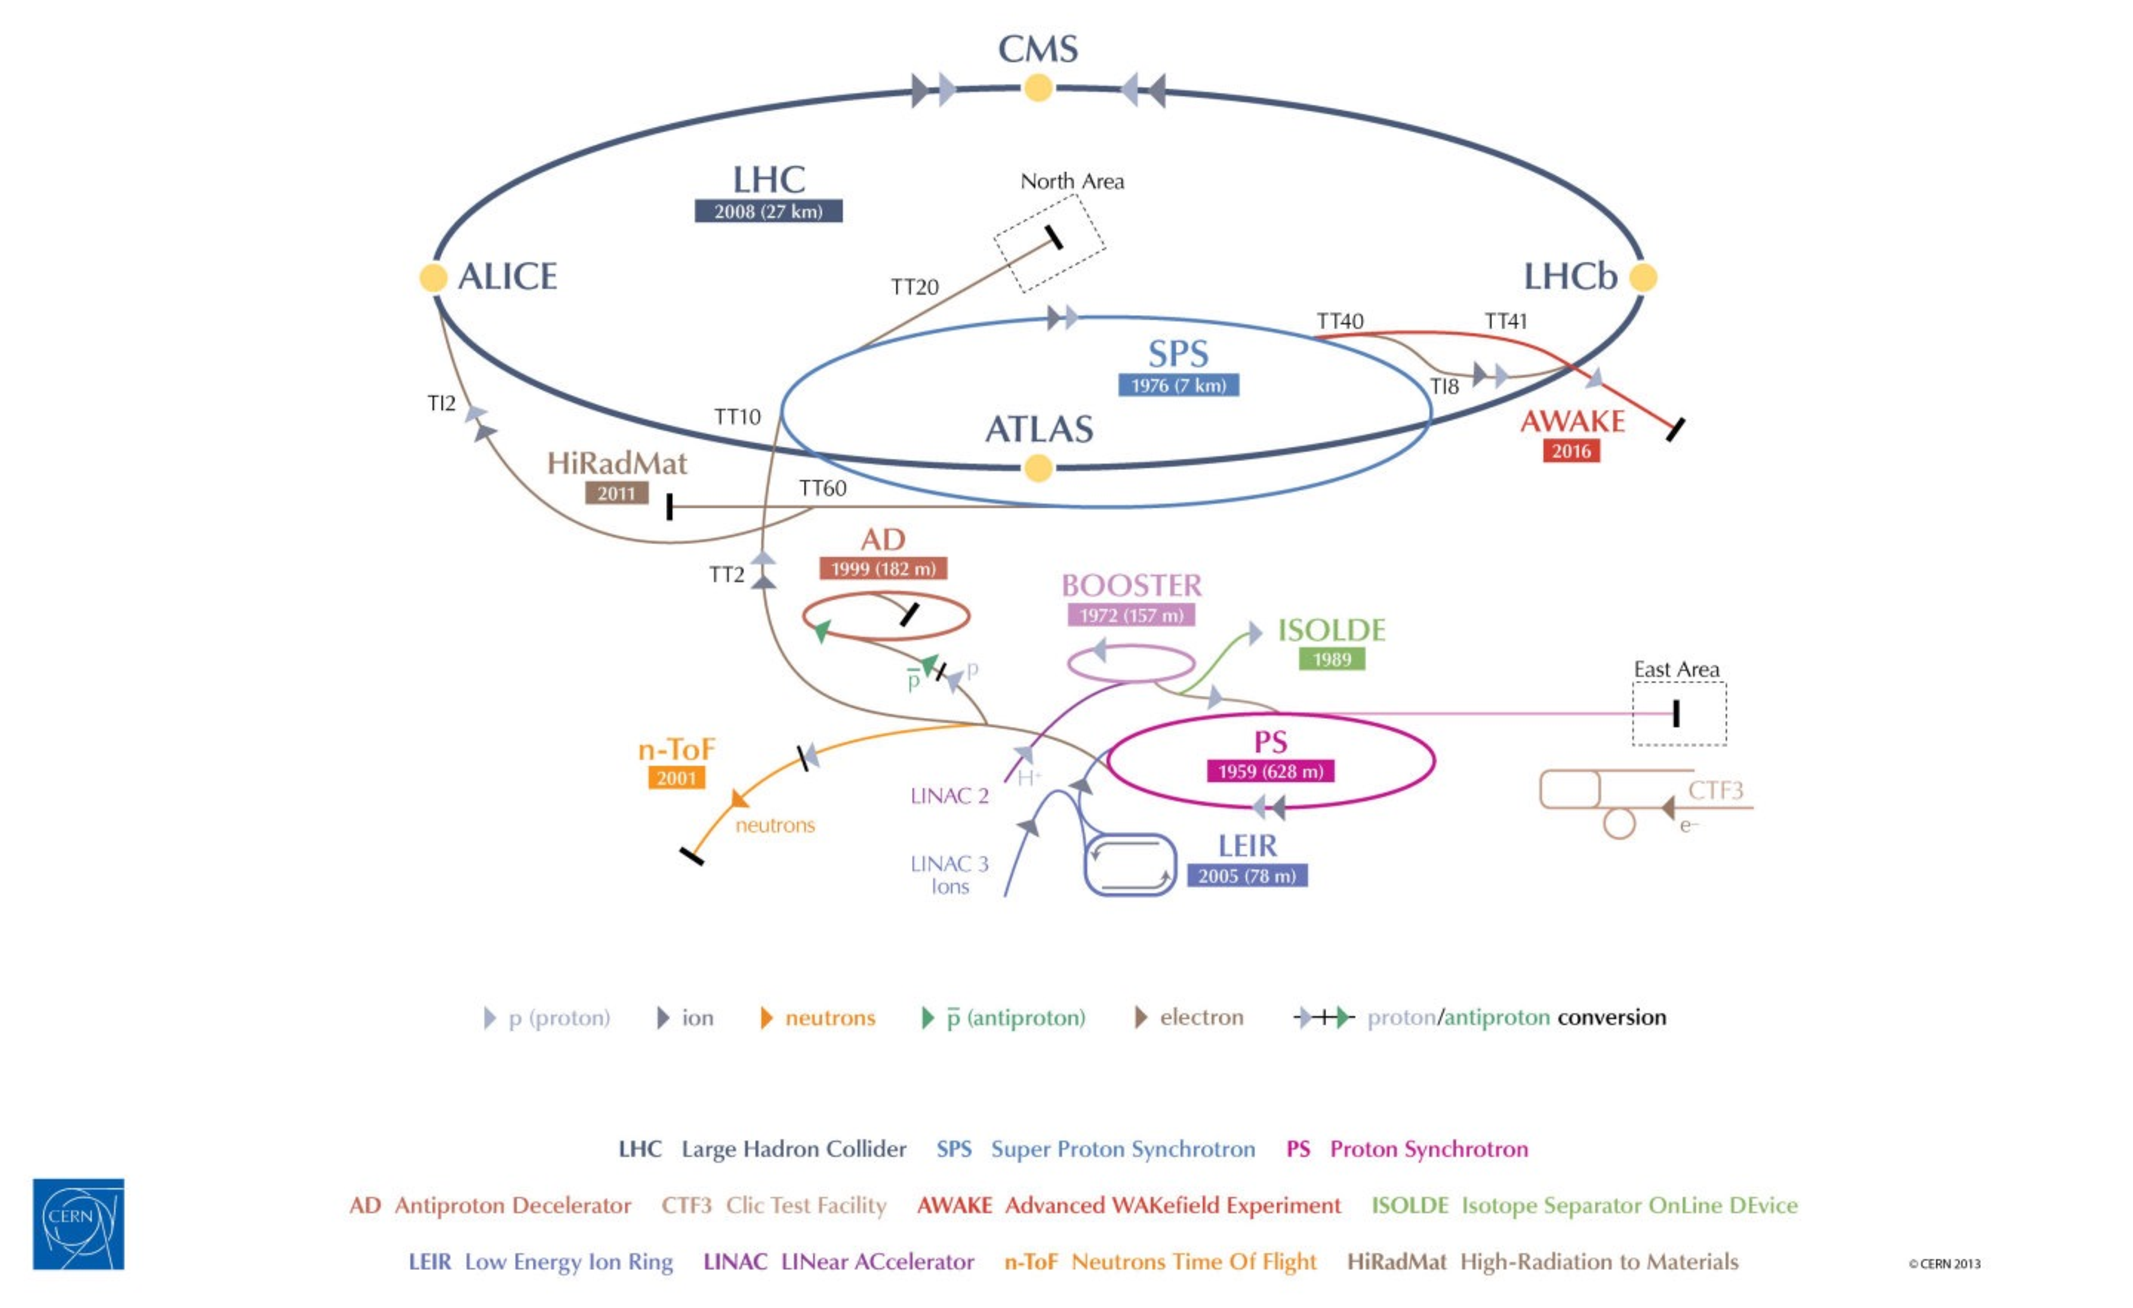
\includegraphics[width=\textwidth]{\chthree/LHC.pdf}
 \end{center}
 \caption{The CERN accelerator complex showing the chain of injection of protons into the LHC ring and the locations of the four main experiments ATLAS, CMS, LHCb and ALICE~\cite{Marcastel:1621583}.}
 \label{fig:LHC}
\end{figure}

LHC operation officially started at the beginning of September 2008 but it was interrupted after a short period, 
due to the breakdown of superconducting magnets. The collider has been reactivated in November 2009 with first pp collisions at $\sqrt{s} = 900\GeV$, officially starting a new era in the particle physics experiments. %Figure~\ref{fig:LHCschedule} shows the LHC timeline together with the phases of its operation. 
The operating center-of-mass energies in pp collisions have so far been 7\TeV in 2010-2011, 8\TeV in 2012 and 13\TeV in 2015-2016. The 7 and 8\TeV periods together make out the \textit{LHC Run~1}, while the 13\TeV period is called the \textit{LHC Run~2}. The work presented in this document is based on data sets collected with pp collisions at 8\TeV in 2012 and at 13\TeV in 2015.

During the whole Run~1, the LHC operated with a 50\unit{ns} bunch spacing.
The peak of instantaneous luminosity in 2011 has been $\approx 0.4\ten{34}\percms$ with a total delivered integrated luminosity of 6.1\fbinv~\cite{LumiPublicResults}.
In 2012 the beam energy increased to 4\TeV per beam with a peak luminosity of $\approx0.8\ten{34}\percms$ and 23.3\fbinv delivered integrated luminosity by the end of that year~\cite{LumiPublicResults}. The increment of the instantaneous luminosity leads to a no more negligible number of simultaneous interactions per bunch crossing, the so-called \textit{pileup} (PU) events. It depends on the cross section of inelastic collisions (75\unit{mb} at $\sqrt{s} = 8\TeV$~\cite{Cartiglia:2013vsa}) and it is directly linked to the instantaneous luminosity. The average PU of the data collected in 2012 is equal to 21 (Fig.~\ref{fig:LHClumiAndPU}) while it has been around 15 in 2011~\cite{LumiPublicResults}.

A long shut-down period for the LHC (LS1) occurred during the whole 2013 and 2014, where upgrades and technical improvements have been performed in order to reach the designed instantaneous luminosity and center-of-mass energy. On March, 21st 2015 the first pp collisions at $\sqrt{s} = 13\TeV$ has been obtained, a new record-breaking energy. For the first three months the machine operated with 50\unit{ns} bunch spacing while, from August 2015, it has been reduced to the designed 25\unit{ns} and the number of bunches per beam has been increased. The first part of this Run~2 phase ended on November 2015 with a total delivered integrated luminosity of 4.2\fbinv and a peak luminosity of $\approx0.5\ten{34}\percms$ with an average pileup of 12~\cite{LumiPublicResults}.

The LHC Run~2 has been restarted in April 2016, after an end-of-the-year technical stop, reaching a peak luminosity of $\approx1.5\ten{34}\percms$. The machine has remained in operation at $\sqrt{s}$ = 13\TeV for the whole year with a total delivered integrated luminosity of 40\fbinv. Accordingly to the current LHC schedule, the Run~2 will proceed up to the end of 2018 with a total expected integrated luminosity of $\approx150\fbinv$. The data collected in 2016 are not considered in this work.

%\textcolor{red}{add some comments about HL-LHC}
%\begin{figure}[h]
% \begin{center}
%  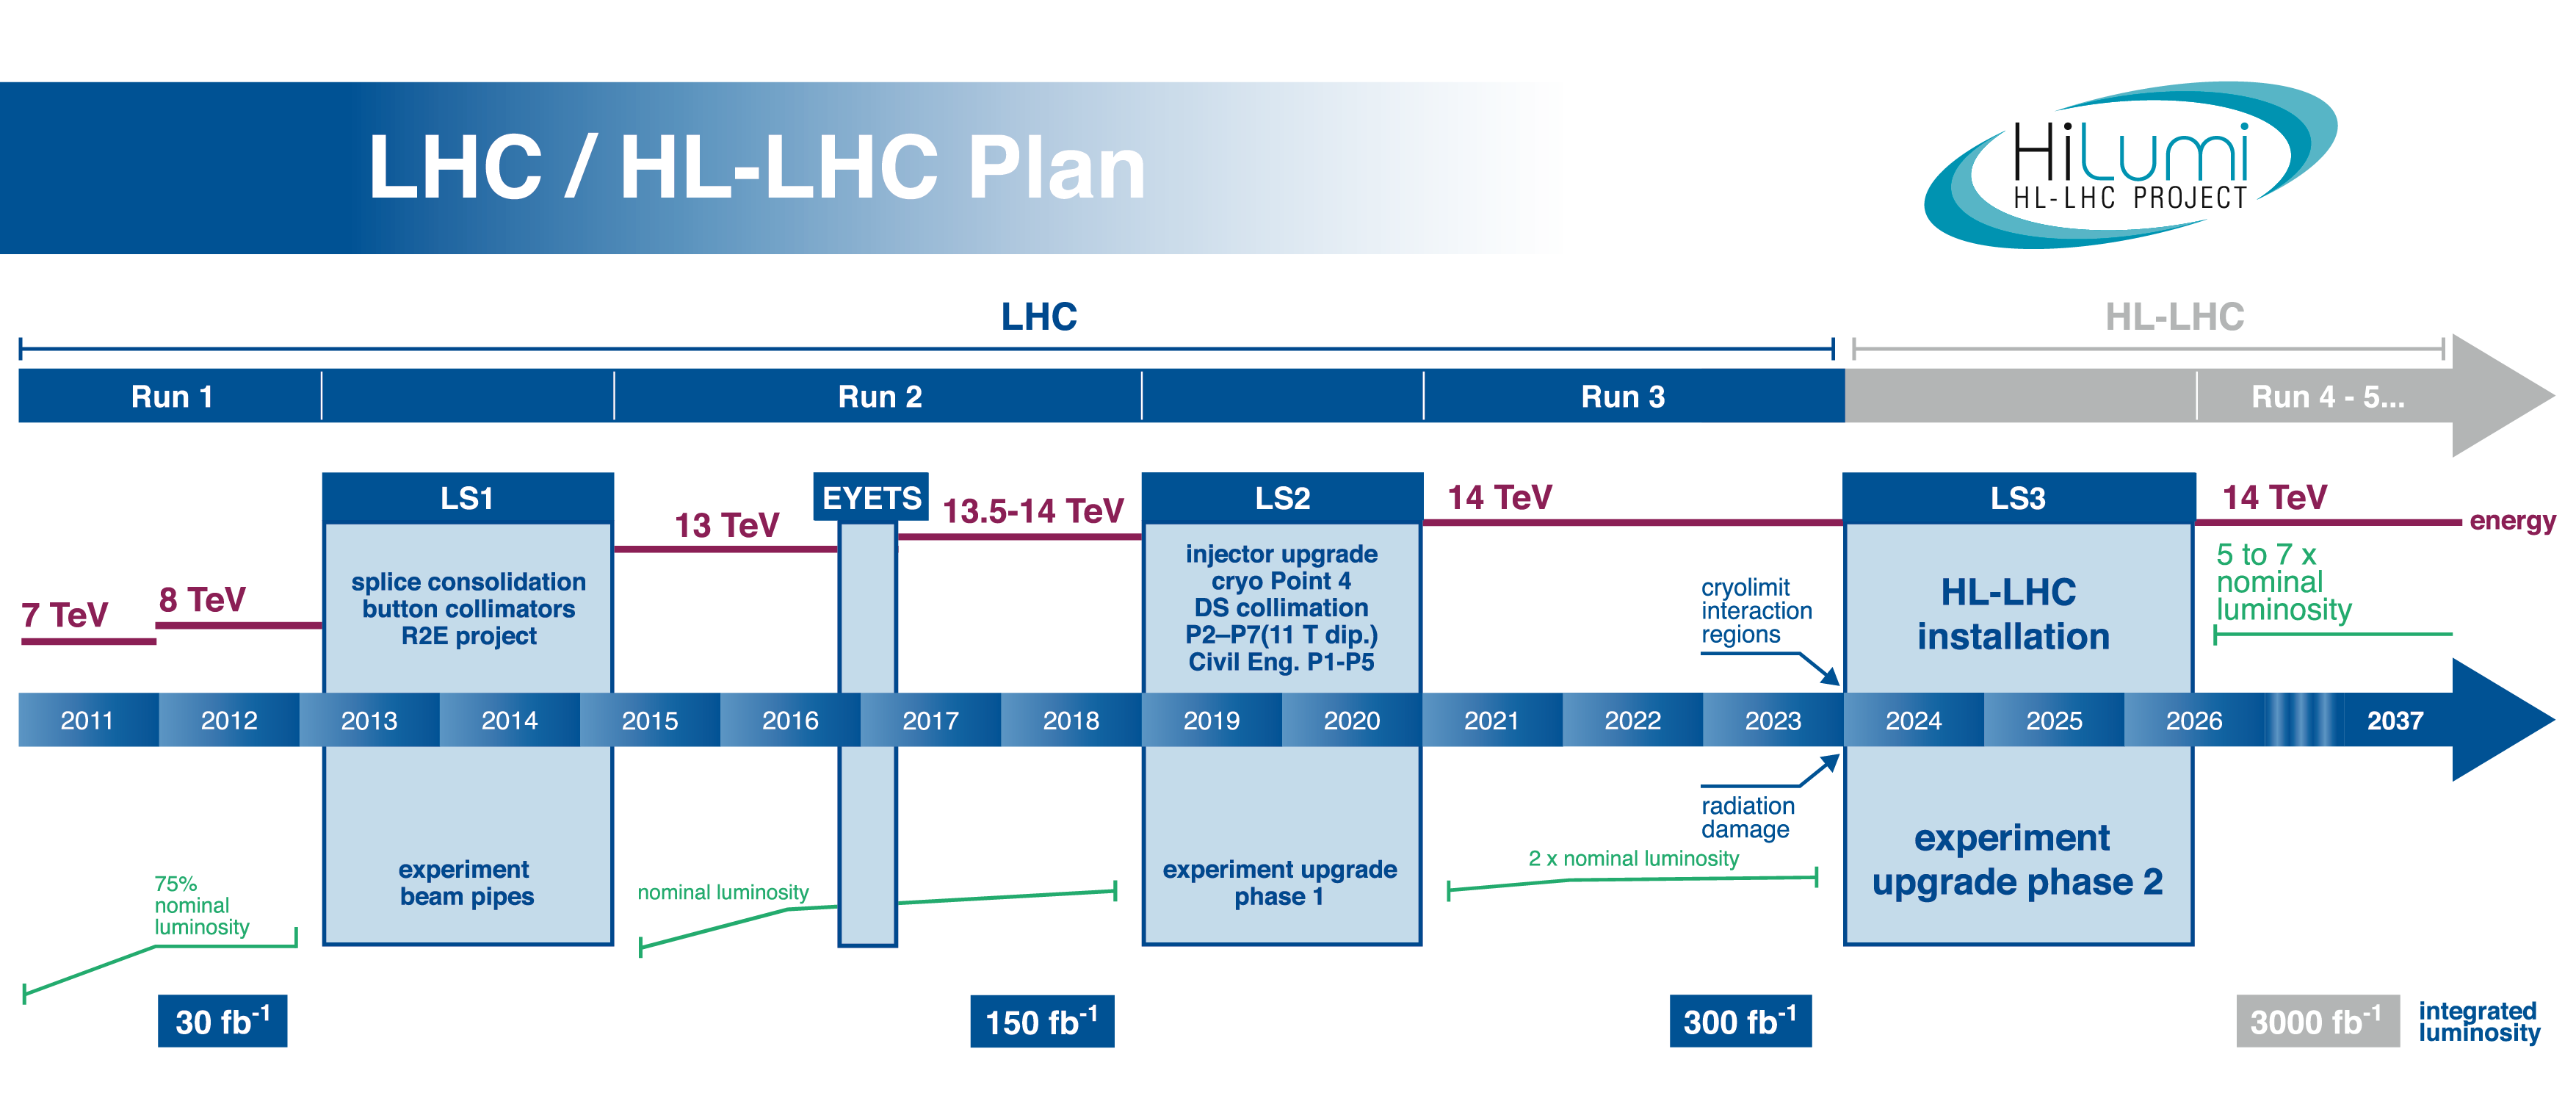
\includegraphics[width=\textwidth]{\chthree/HL-LHC-plan-2016-01.png}
% \end{center}
% \caption{LHC timeline.}
% \label{fig:LHCschedule}
%\end{figure}

\begin{figure}[!htb]
 \begin{center}
 \subfigure[]{\label{fig:LHClumiAndPU_a}\includegraphics[width=0.48\textwidth]{\chthree/pileup_pp_2012.png}}
 \subfigure[]{\label{fig:LHClumiAndPU_b}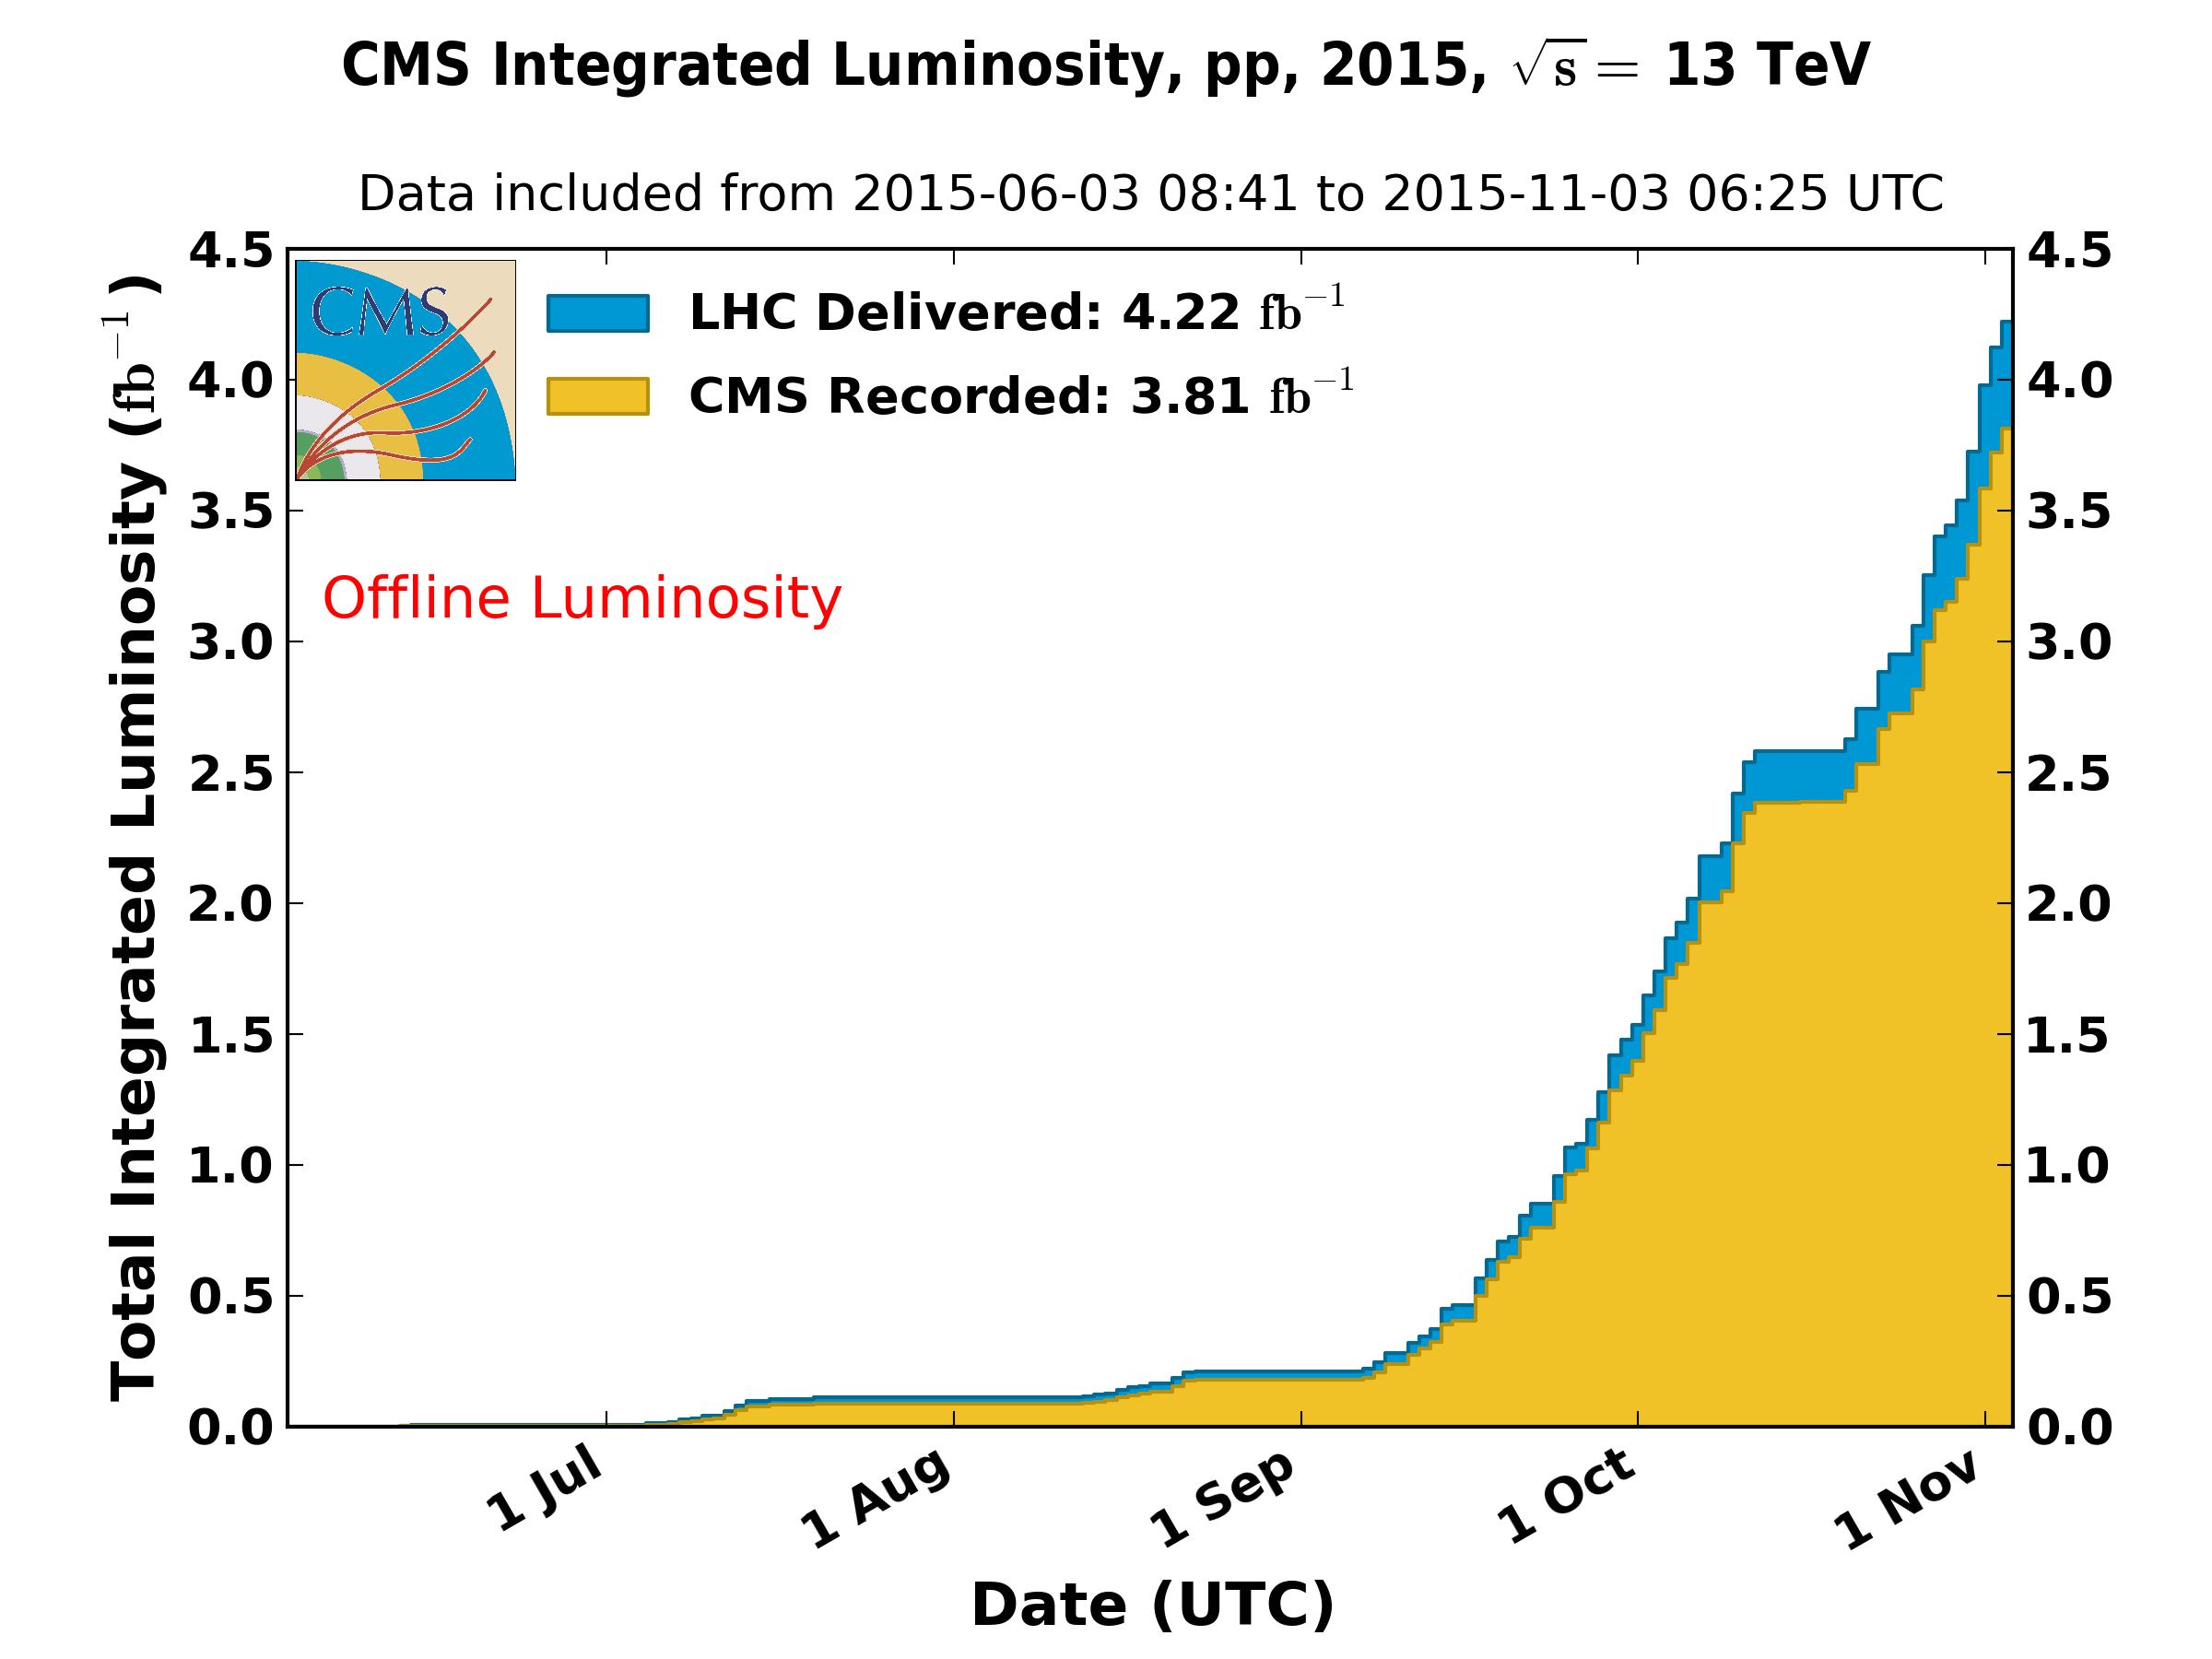
\includegraphics[width=0.48\textwidth]{\chthree/int_lumi_per_day_cumulative_pp_2015.png}}
 \end{center}
 \caption{(a) Number of simultaneous interactions per bunch crossing in data collected in 2012 by the CMS experiment at LHC. (b) Cumulative luminosity versus day delivered by LHC (blue) in 2015; the offline luminosity recorded by the CMS experiment is also reported (orange).~\cite{LumiPublicResults}}
 \label{fig:LHClumiAndPU}
\end{figure}

%\begin{figure}[h]
% \begin{center}
%  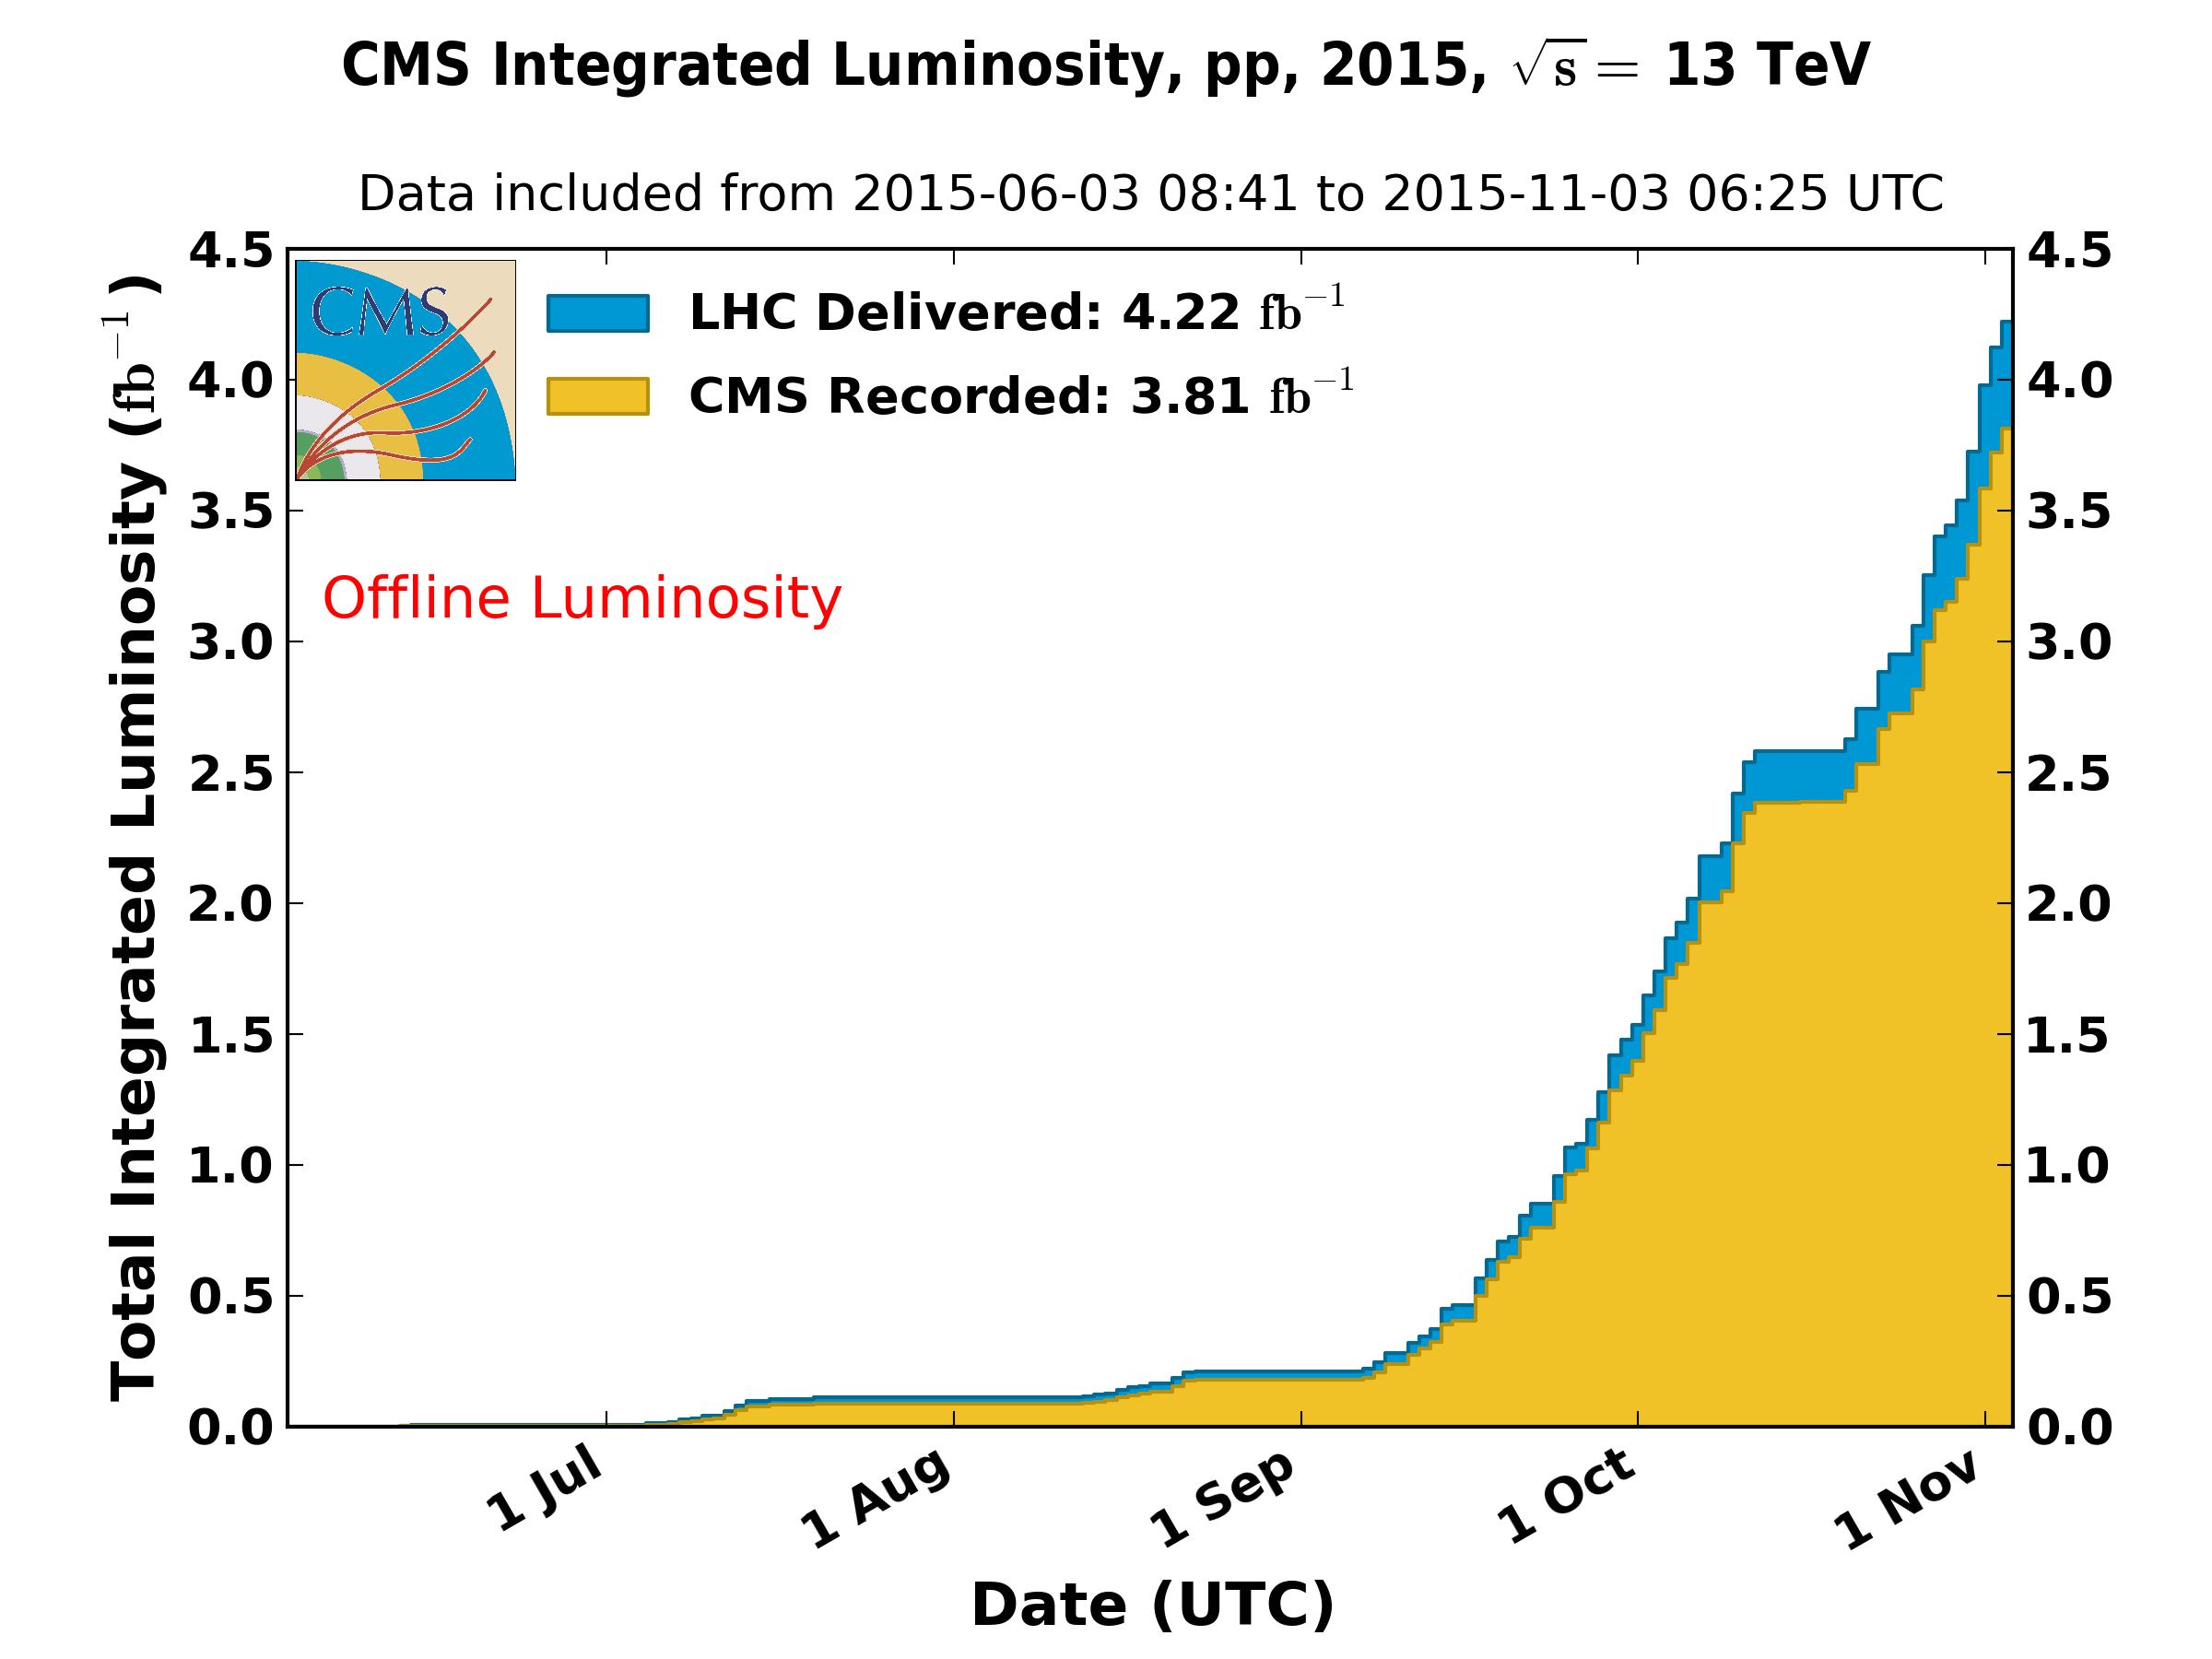
\includegraphics[width=0.45\textwidth]{\chthree/int_lumi_per_day_cumulative_pp_2015.png}
   %\includegraphics[height=11cm,width=0.5\textwidth]{chapters/Chapter3-CMSatLHC/Figurues/pileup_pp_2012.png}
% \end{center}
% \caption{Integrated lumi and PU for 2015.}
% \label{fig:LHCRun2}
%\end{figure}

%\section{The CMS Detector}
    \section{The CMS detector}
\label{sec:CMSdetector}

The CMS detector is a general purpose detector installed 100\unit{m} underground at the LHC interaction point 5 (P5) near the village of Cessy in France.
It has been designed to exploit the different properties of the wide range of particles and physics processes produced in high-energy collisions at the LHC.\\

The design of this detector is driven by the challenges of a physics experiment in the LHC environment. 
Many of the physics processes of interest have a small cross section and the background from QCD jet production is overwhelmingly dominant.
In order to achieve an optimal efficiency for rare channels and high rejection power for QCD background, the detector has to be able to reconstruct the primary interaction entirely
and to reduce the influence of overlapping interactions on its reconstruction.
Therefore, one needs to collect all the relevant information on the particles passing through the detector. Since these have different properties, a mixture of subdetectors is required for a complete event reconstruction. The reconstruction of lepton signatures is essential for the extraction of rare processes. An excellent muon and electron identification and momentum resolution is therefore desired. A precise measurement of secondary vertices and track impact parameters is fundamental for an efficient identification of heavy flavor quarks and $\tau$ leptons. Moreover, a large hermetic geometric coverage is preferred, which allows for a precise estimate of the transverse momentum carried away by invisible particles by reconstructing the missing momentum of all of the visible particles.

The high peak luminosities of the LHC lead to a large number of PU interactions, imposing further challenges to the design. As a consequence of pileup, the products of an interaction under study may be confused with those from other interactions in the same bunch crossing. This effect can be reduced by using high-granularity detectors resulting in low occupancy per recorded event. In addition, the short bunch crossing period requires fast response time and good time resolution of each detector element.
%in order to discriminate the interaction under study from the interactions occurring in neighbouring bunch crossings.
Hence, a large number of detector channels and an excellent synchronization among them are necessary. Another challenge arises from the large flux of particles near the interaction point which leads to high radiation levels and the need of radiation-hard detectors and front-end electronics.\\

Figure~\ref{fig:CMSlayout} shows the layout of the CMS detector. The detector is built in a cylindrical structure composed of a barrel in the center and endcaps at both sides. This structure is 21.6-m-long, 14.6\unit{m} in circumference and has a mass of 12500 tons. The detector design and layout was driven by the choice of the magnetic field configuration. Large bending power is needed for a precise measurement of the momentum of high-energy charged particles. Within the CMS detector this is achieved by a superconducting solenoid with a length of 12.9\unit{m} and an inner diameter of 5.9\unit{m} generating a magnetic field of 3.8\unit{T}. The bore of the magnet coil is large enough to accommodate the inner tracker and the calorimetry inside. 
The inner tracker consists of silicon pixel and strip detectors, representing the key component of CMS to measure the momenta of charged particles and identify primary and secondary vertices. The calorimetry system is comprised of a crystal electromagnetic calorimeter (ECAL) and a brass and scintillator hadronic calorimeter (HCAL), which provide information on the energies and directions of all charged and neutral particles. Outside the magnet are the large muon detectors, which, integrated inside the return yokes of the magnet, provide identification of muons and measurement of their momenta.\\

For the description of the CMS detector the following coordinate system is used. The origin is centered at the nominal collision point inside the experiment with the $y$-axis pointing vertically upward, the $x$-axis pointing radially inward toward the center of the LHC, and the $z$-axis pointing along the beam direction. The azimuthal angle $\phi$ is measured from the $x$-axis in the $x$-$y$ plane. The polar angle $\theta$ is measured from the $z$-axis. Pseudorapidity is defined as $\eta = -\ln\tan(\theta/2)$. Thus, the momentum and energy measured transverse to the beam direction, denoted by \PT and \ET, respectively, are computed from the $x$ and $y$ components.\\

In the following sections the three main components of the CMS detector will be described together with a section on the triggering system.

\begin{figure}[!htb]
 \begin{center}
  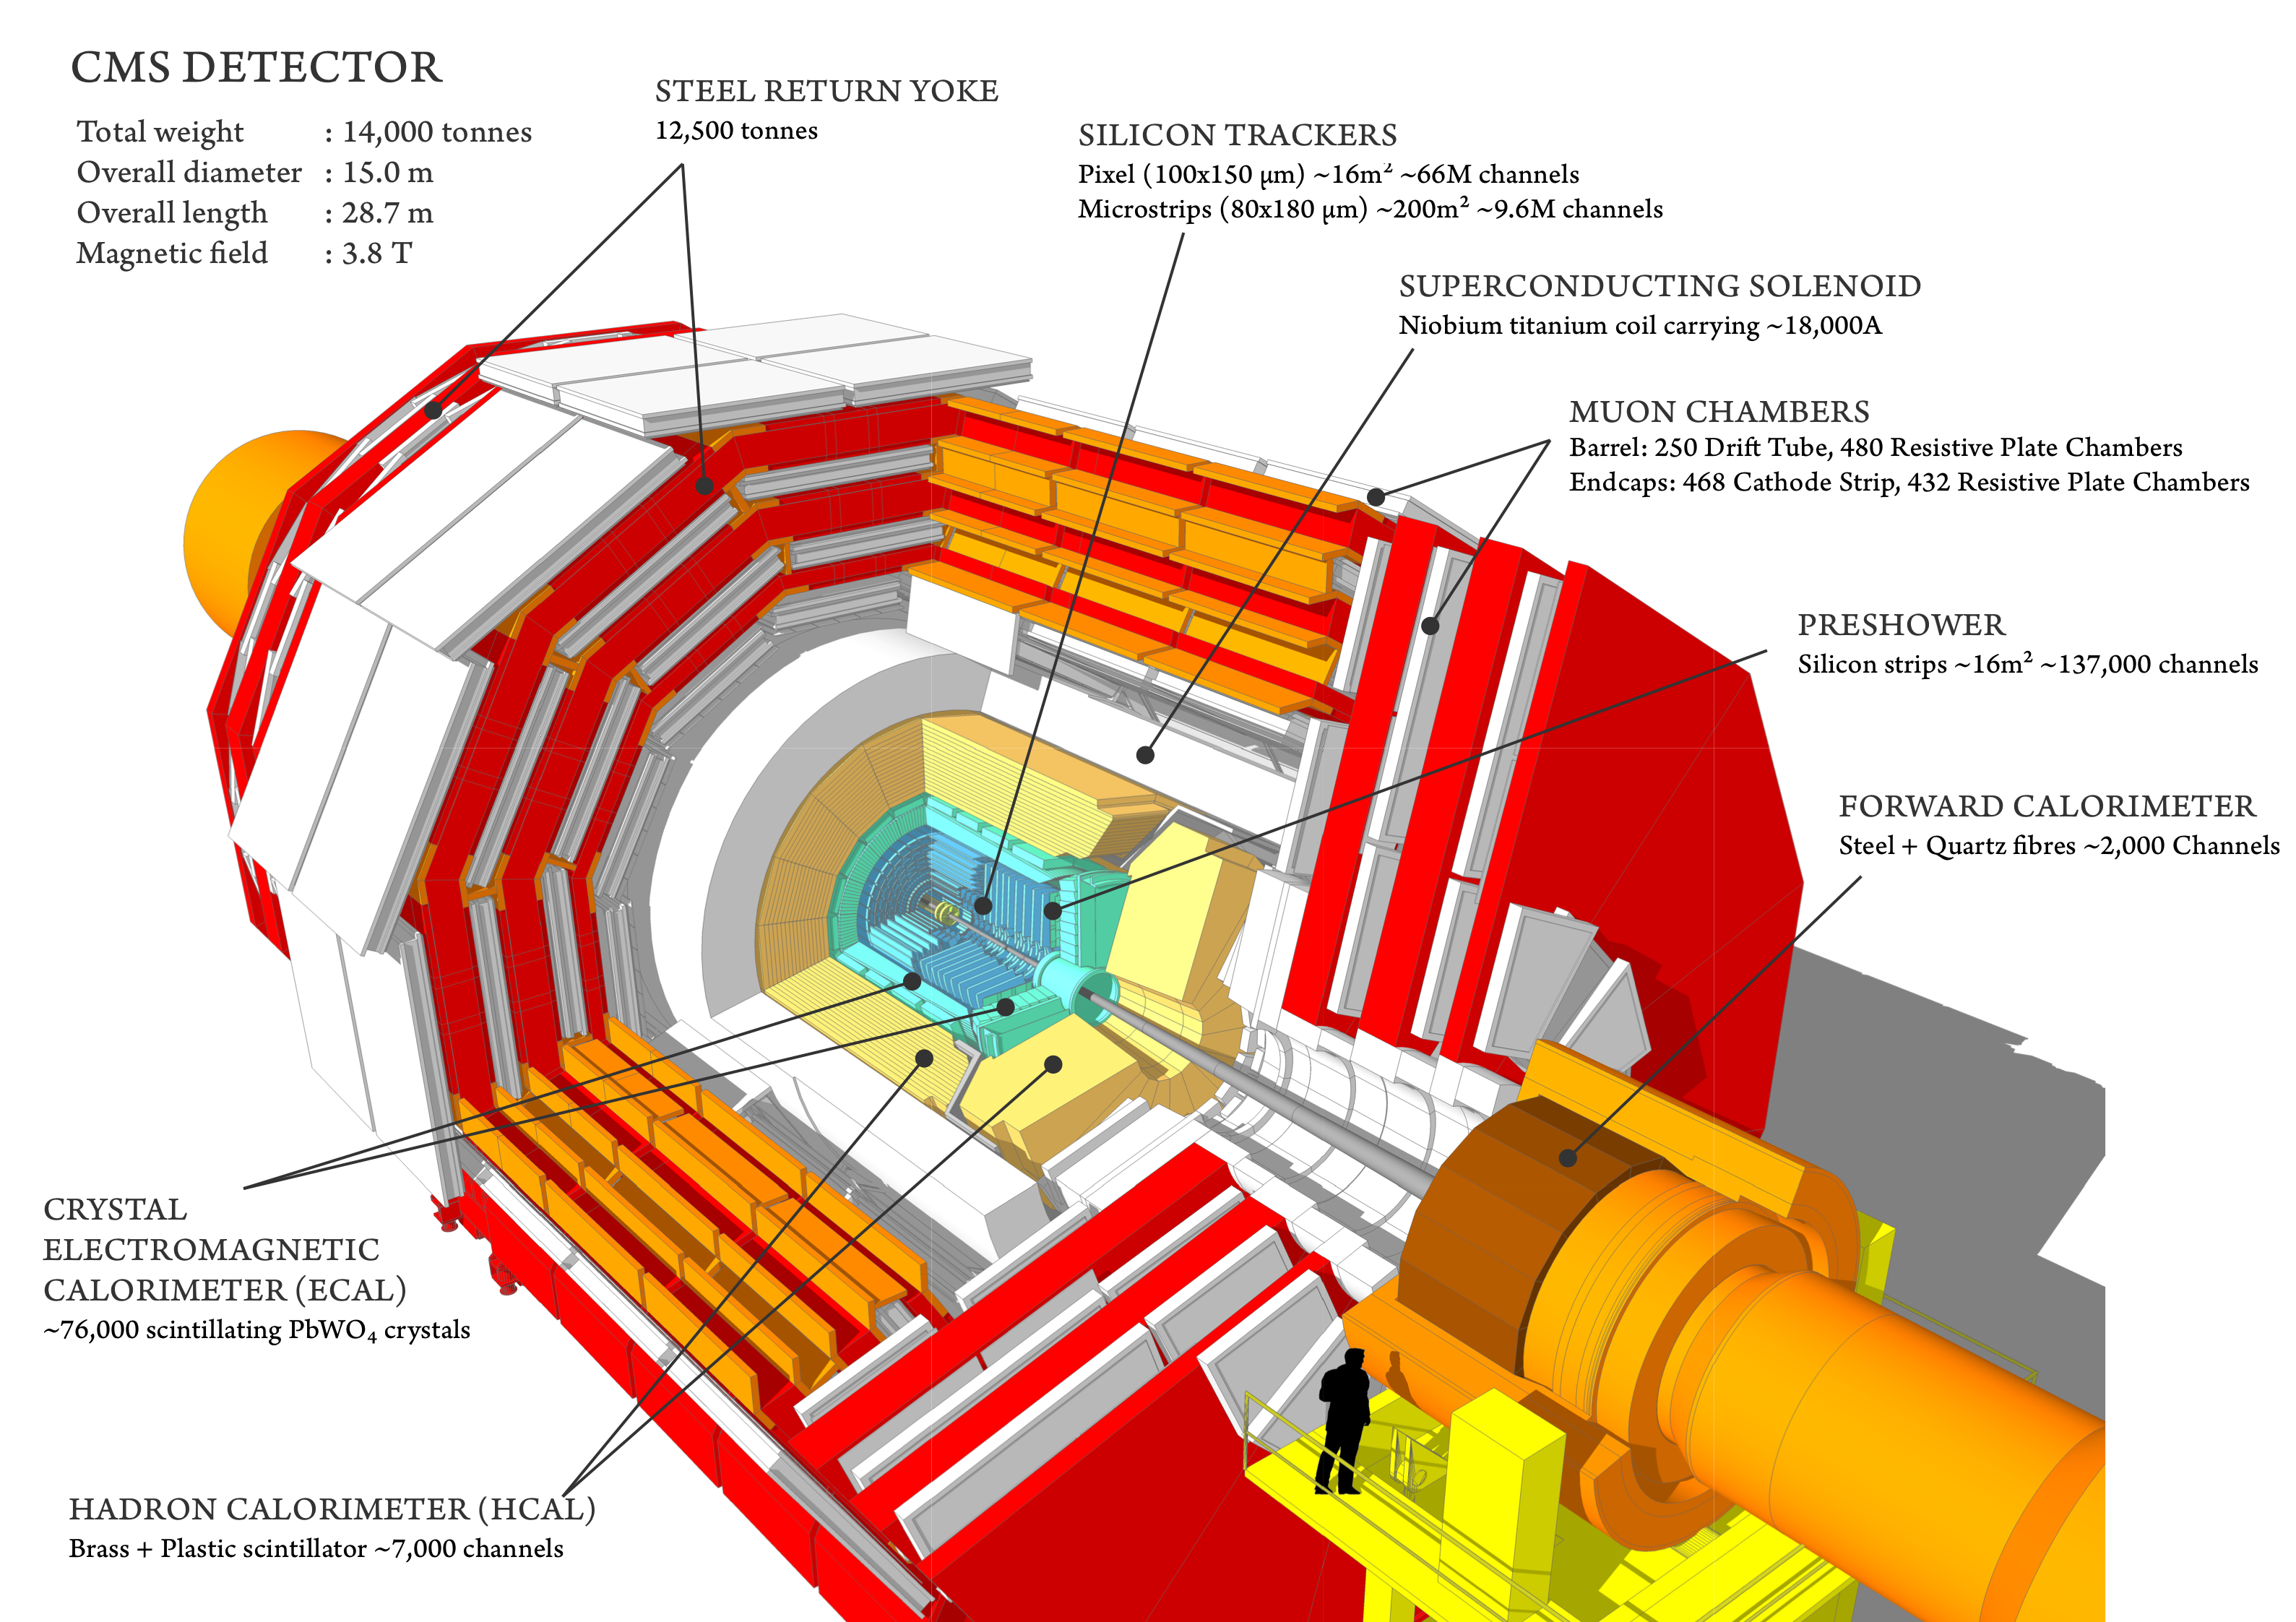
\includegraphics[width=0.9\textwidth]{\chthree/cms_120918_03.png}
 \end{center}
 \caption{Layout of the CMS experiment and its subdetectors.}
 \label{fig:CMSlayout}
\end{figure}

%%%%%%%%
\subsection{Tracking detectors}
%%%%%%%%

The tracking system of CMS (Fig.~\ref{fig:TrackerLayout}) is designed to provide a precise and efficient measurement of the trajectories of charged particles emerging from the LHC collisions, as well as a precise reconstruction of secondary vertices~\cite{Karimaki:368412}. It surrounds the interaction point and has a length of 5.8\unit{m} and a diameter of 2.5\unit{m} providing coverage up to $|\eta| < 2.5$. In order to achieve high tracking efficiency at the high luminosities of LHC, a detector technology featuring granularity, speed and radiation hardness is required. Furthermore, the material budget of the tracking system has to be as low as possible in order to avoid a worsening of the tracking efficiency and resolution due to material interaction effects of the charged particle, such as multiple scattering, bremsstrahlung, photon conversion and nuclear interactions. These requirements lead to a tracker design entirely based on silicon detector technology. With about 200\unit{m$^2$} of active silicon area the CMS tracker is the largest silicon tracker ever built. It is divided into a pixel detector close to the interaction region and a strip detector in the outer region. The motivations for this layout are explained in what follows.

At LHC design luminosity more than 1000 particles are hitting the tracking volume in each bunch crossing. This leads to a hit rate density of 1\unit{MHz/mm$^2$} at a radius of 4\cm which imposes severe challenges to the design of the tracking detectors. With a pixel size of $100\times150$\unit{$\mu\mathrm{m}^2$} in $r$-$\phi$ and $z$, respectively, an occupancy of the order of $10^{-4}$ per pixel per LHC bunch crossing can be achieved. The hit rate density falls with the distance from the interaction point to 60\unit{kHz/mm$^2$} at a radius of 22\cm and to 3\unit{kHz/mm$^2$} at a radius of 115\cm. Therefore, at intermediate radii (20--55\cm), silicon micro-strip detectors are used, with a typical cell length of 10\cm and a pitch of 80\mum. At the outermost radii (55-110\cm)
the strip size can be further increased to $25\cm\times180\mum$. With this choice an occupancy of less than 3\% is maintained in the strip detector.
However, the strip capacitance scales with its length and therefore the electronics noise is a linear function of the strip length as well, becoming not negligible in the outermost region where the strip size is the largest. In order to maintain a good signal to noise ratio well above 10, CMS uses thicker silicon sensors for the outer tracker region (500\mum thickness as opposed to the 320\mum in the inner tracker) with correspondingly higher signal. To mitigate the radiation damage effects and prolong the lifetime of the detector modules, the tracking detectors are designed to run at subzero temperatures. The cooling is established using a mono-phase liquid cooling system with C$_6$F$_{14}$ as cooling fluid. The whole tracker system operated at +4\de\unit{C} during Run~1. After this phase, several improvements were implemented and an operative temperature of -15\de\unit{C} is currently maintained for Run~2.\\

\begin{figure}[!htb]
 \begin{center}
  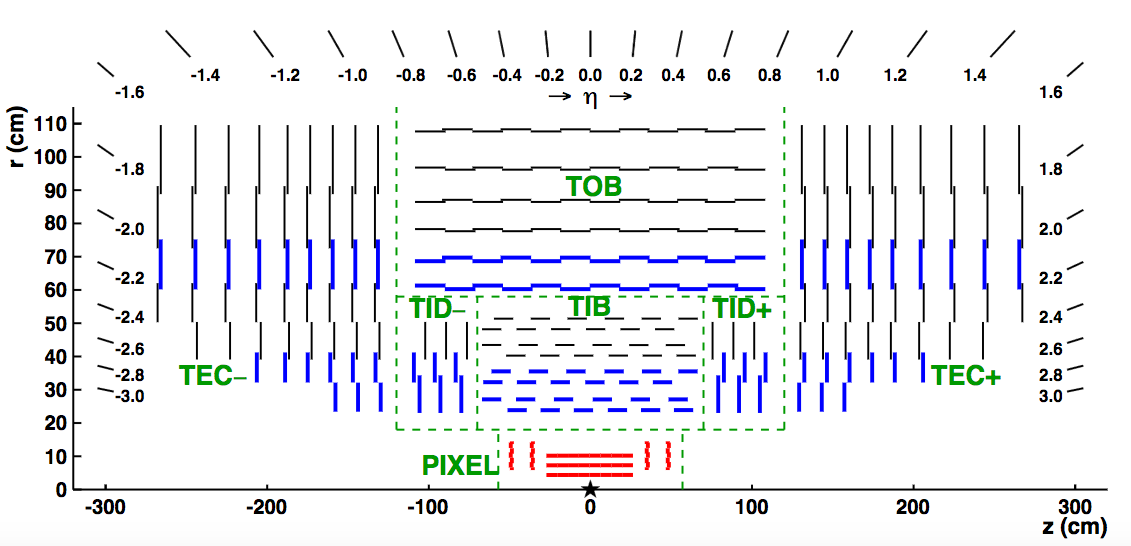
\includegraphics[width=0.8\textwidth]{\chthree/tracker.png}
 \end{center}
 \caption{Longitudinal section of half of the original CMS silicon tracker system; the different detector types are indicated.}
 \label{fig:TrackerLayout}
\end{figure}

The original pixel detector is built from 3 barrel layers at radii of 4.4, 7.3 and 10.2\cm (BPix) and two end disks (FPix) on each side at a distance of $z$ = $\pm$34.5, $\pm$46.5\cm from the interaction point. It consists of 1440 segmented silicon sensor modules with a total of 66 million readout channels covering an area of about 1\unit{m$^2$}. The pixel detector is essential for the reconstruction of the primary and pileup vertices, as well as of the secondary vertices from the decay of bottom quarks and $\tau$ leptons. It provides precise track point measurements in $r$-$\phi$ and $z$ and therefore guarantees a small impact parameter resolution important for good secondary vertex reconstruction. This is achieved thanks to the readout of the analog pulse height information. The sensor surface in the barrel layers is parallel to the magnetic field, hence the charge carriers produced by a particle traversing experience a Lorentz drift, which leads to charge spreading over more than one pixel (``charge-sharing''). The analog pulse height information can be used to calculate a center of gravity of the charge distribution improving the hit information. The forward FPix disks are tilted at 20\de in a turbine-like geometry to induce charge-sharing. As shown in Fig.~\ref{fig:pxRes}, a spatial resolution of 10\mum in the transverse plane and 30\mum in the longitudinal direction can be achieved for BPix. For FPix a spatial resolution of 20\mum is obtained in both directions. %FROM TDR: A spatial resolution of approximately 15~$\mu$m in both the $r$-$\phi$ and $z$ directions can be achieved with charge-sharing between neighboring pixels. 
A detailed description of the design and the functioning of the CMS pixel barrel detector is given in Chapter~\ref{ch:BPix}.\\

\begin{figure}[h]
 \begin{center}
\subfigure[]{\label{fig:pxRes_a}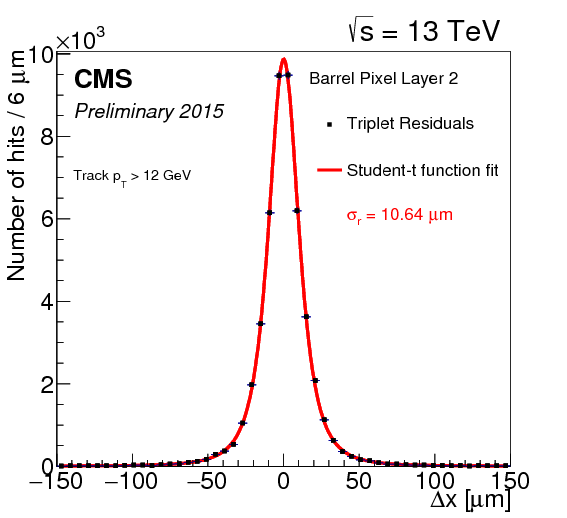
\includegraphics[width=0.48\textwidth]{\chthree/PixelResolution_dx.png}}
\subfigure[]{\label{fig:pxRes_b}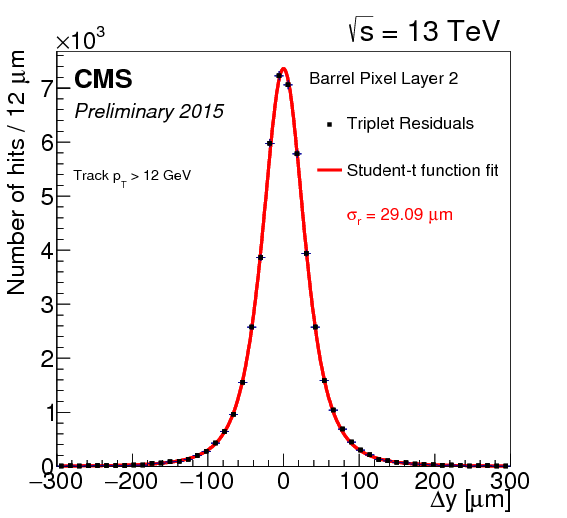
\includegraphics[width=0.48\textwidth]{\chthree/PixelResolution_dy.png}}
 \end{center}
 \caption{Distributions of the hit residuals on the pixel barrel layer 2 in the transverse (a) and longitudinal (b) direction with respect to the beam. The distributions are fitted with a Student's t-function. The fitted width parameter $\sigma_\mathrm{r}$ is reported on the plot~\cite{PixelOffline}.}
 \label{fig:pxRes}
\end{figure}

The strip detector occupies the radial region between 20\cm and 1.16\unit{m}. As illustrated in Fig.~\ref{fig:TrackerLayout}, it is composed of four subsystems: the four-layer Tracker Inner Barrel (TIB), the six-layer tracker outer barrel (TOB) and on each side three-disk Tracker Inner Disks (TID) and nine-disk Tracker Endcaps (TEC). The silicon micro-strip sensors have strips parallel to the beam axis in the barrel and radially on the disks. The modules in the first two layers and rings, respectively, of TIB, TID, and TOB as well as rings 1, 2, and 5 of the TECs carry a second micro-strip detector module which is mounted back-to-back with an angle of 100\unit{mrad} in order to provide a measurement of the second coordinate ( $z$ in the barrel and $r$ on the disks). This tracker layout ensures at least 9 hits in the silicon strip tracker in the full range $|\eta| < 2.4$ with at least 4 of them being two-dimensional measurements. The total number of silicon sensors in the strip tracker is 24244, making up a total active area of 198\unit{m$^2$}, with about 9.3 million of strips.
%TIB/TID
%The Tracker Inner Barrel and Disks (TIB/TID) extend in radius towards 55 cm and are composed of 4 barrel layers, supplemented by 3 disks at each end. TIB/TID delivers up to 4 $r$-$\phi$ measurements on a trajectory using 320 $\mu$m thick silicon micro-strip sensors with their strips parallel to the beam axis in the barrel and radial on the disks.  The strip pitch is 80 $\mu$m on layers 1 and 2 and 120 $\mu$m on layers 3 and 4 in the TIB, leading to a single point resolution of 23 $\mu$m and 35 $\mu$m, respectively.
%In the TID the mean pitch varies between 100 $\mu$m and 141 $\mu$m.
%TOB
%The TIB/TID is surrounded by the Tracker Outer Barrel (TOB). It has an outer radius of 116 cm and consists of 6 barrel layers of 500 $\mu$m thick micro-strip sensors with strip pitches of 183
%$\mu$m on the first 4 layers and 122 $\mu$m on layers 5 and 6. It provides another 6 $r$-$\phi$ measurements with single point resolution of 53 $\mu$m and 35 $\mu$m, respectively. 
%The TOB extends in $z$ between $\pm$ 118 cm. 
%TEC
%Beyond this $z$ range the Tracker EndCaps (TEC+ and TEC- where the sign indicates the location along the $z$ axis) cover the region 124 cm < |$z$| < 282 cm and 22.5 cm < |$r$| < 113.5 cm. Each TEC is composed of 9 disks, carrying up to 7 rings of silicon micro-strip detectors (320 $\mu$m thick on the inner 4 rings,  500 $\mu$m thick on rings 5-7) with radial strips of 97 $\mu$m to 184 $\mu$m average pitch. Thus, they provide up to 9 $\phi$ measurements per trajectory.
%In addition, the modules in the first two layers and rings, respectively, of TIB, TID, and TOB as well as rings 1, 2, and 5 of the TECs carry a second micro-strip detector module which is
%mounted back-to-back with a stereo angle of 100 mrad in order to provide a measurement of the second co-ordinate ( $z$ in the barrel and $r$ on the disks). The achieved single point resolution of this measurement is 230 $\mu$m and 530 $\mu$m in TIB and TOB, respectively, and varies with pitch in TID and TEC. This tracker layout ensures at least 9 hits in the silicon strip tracker in the full range of |$\eta$| < 2.4 with at least 4 of them being two-dimensional measurements (figure 3.2).

%%%%%%%%
\subsection{Calorimetry}
%%%%%%%%

The calorimeter measures the energies and directions of all neutral and charged particles traversing the detector, with the exception of muons and neutrinos. It consists of two parts, the
electromagnetic calorimeter (ECAL)~\cite{ECALtdr} and the hadronic calorimeter (HCAL)~\cite{HCALtdr}.\\

The goal of the ECAL is to measure precisely the energy of electrons and photons which generate electromagnetic showers inside it. It is a hermetic and homogeneous calorimeter with a large pseudorapidity coverage up to $|\eta| < 3$. As illustrated in Fig.~\ref{fig:ECALLayout}, the ECAL is divided into barrel and endcap detectors consisting of scintillation crystals made from lead tungstate (PbWO$_4$). The choice of this material is motivated by its high density (8.28\unit{g/cm$^3$} ), short radiation length ($X_0$ = 0.89\cm) and small Moli\`{e}re radius (2.2\cm), resulting in high stopping power, fine granularity and a compact size that fits inside the solenoid.
The ECAL comprises 61200 crystals in the barrel and 7324 crystals in each of the 2 endcaps, for a total volume of 8.14\unit{m$^3$} and 2.9\unit{m$^3$}, respectively. The crystals have a tapered shape and are mounted in a quasi-projective geometry.
The barrel extends radially between 1.29 and 1.75\cm covering the region $|z| < 3.05\unit{m}$ and $|\eta| < 1.479$. The crystals have a front face cross-section of $22\times22$\unit{mm$^2$} and a length of 2.3\cm (25.8 $X_0$). They are organized in 36 identical supermodules each covering 20\de in $\phi$. The crystals are contained in thin-walled glass-fibre alveola structures (``submodules'') with $2(\phi)\times5(\eta)$ crystals each resulting in a granularity 360-fold in $\phi$ and $2\times85$-fold in $\eta$. The endcaps are placed at a distance of 3.14\unit{m} from the interaction point and they extend radially between 3.16 and 17.11\cm, covering the region $1.479 < |\eta| < 3.0$. The crystals have a front face cross section of $28.6\times28.6$\unit{mm$^2$} and a length of 2.2\cm (24.7 $X_0$). A preshower detector with a thickness of 3 $X_0$ is placed in front of the endcaps ($1.653 < |\eta| < 2.6$) to guarantee a reliable discrimination of single photons and photons produced in pairs from neutral pion decays.
The relatively low light yield of the crystals (30\unit{$\gamma$/\MeV}) requires use of photodetectors with intrinsic gain that can operate in a magnetic field. Silicon avalanche photodiodes (APDs) are used as photodetectors in the barrel and vacuum phototriodes (VPTs) in the endcaps. The light output and the amplification have a strong temperature dependence. The response to an incident electron changes by $(3.8\pm0.4)\%/\de\unit{C}$ which in turn means that the temperature has to be closely monitored and kept stable to a precision of $\pm0.05\de\unit{C}$. The nominal operating temperature of the ECAL is $18\de\unit{C}$ and is provided by a water cooling system.

The energy resolution of the electromagnetic calorimeter can be parametrized by the following expression:

\begin{equation}
\frac{\sigma_E}{E} = \frac{S}{\sqrt{E(\GeV)}} \oplus \frac{N}{E(\GeV)} \oplus C.
\end{equation}

The first term is stochastic, including contributions from the shower containment, the number of photoelectrons and
the fluctuations in the gain process. The second contribution corresponds to the noise term, which includes noise in the readout electronics and fluctuations in pileup.
The third term is a constant dominating the energy resolution for high-energy electron and photon showers. It depends
on non-uniformity of the longitudinal light collection, energy leakage from the back of the calorimeter, single-channel response uniformity and stability. 
The values of the three coefficients were determined by measurements with an electron beam in a matrix of $3\times3$ crystals to be S = 2.8\%, N = 12\% and C = 0.3\%~\cite{1748-0221-2-04-P04004}.\\
%This result was obtained reconstructing the showers in a matrix of 3$\times$3 crystals where the electron impact point on the calorimeter was tightly localized in a region of 4 mm $\times$ 4 mm to give maximum containment of the shower energy within the 3$\times$3 crystal matrix.  

\begin{figure}[!htb]
 \begin{center}
  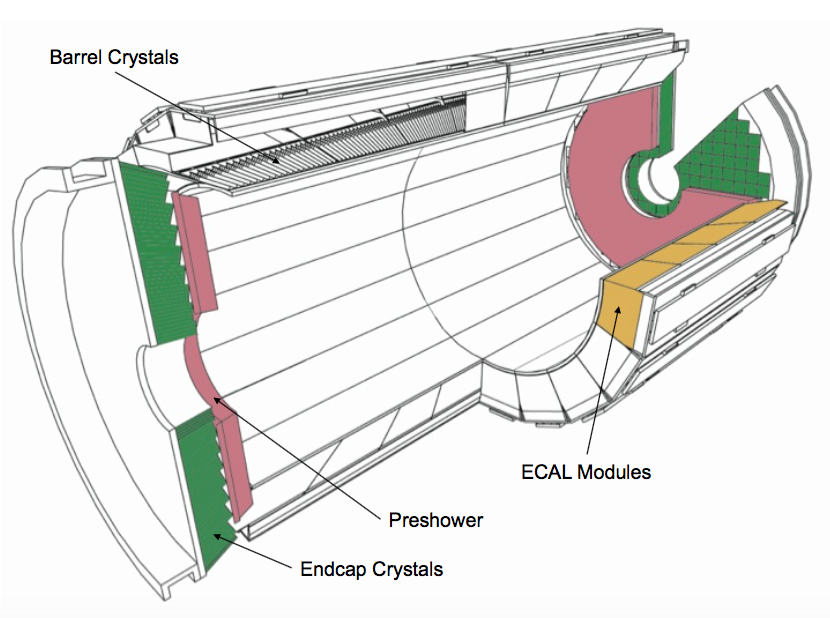
\includegraphics[width=0.8\textwidth]{\chthree/ECAL.png}
 \end{center}
 \caption{Schematic view of the CMS electromagnetic calorimeter~\cite{Chatrchyan:2008zzk}.}
 \label{fig:ECALLayout}
\end{figure}

The energy measurement of the ECAL is complemented by the measurement of the hadronic calorimeter.
%which aims at measuring the energy of the individual hadrons produced in each collision.
The HCAL is designed to be as near to hermetic around the interaction region as possible to allow events with missing energy to be identified.
It is a sampling calorimeter composed of layers of brass absorber interlaced with tiles of plastic scintillators as active material to detect the showers generated by the hadrons in the brass. The energy released in the scintillator tiles causes them to emit blue-violet light, a fraction of which is absorbed and re-emitted by embedded wavelength-shifting fibres in the green region of the spectrum. The green light is then carried by special fibre-optic waveguides to the readout system. The photodetection readout is based on multi-channel hybrid photodiodes (HPDs), which are photodetectors configured especially for CMS that can provide gain and operate in a high magnetic field.

Figure~\ref{fig:HCALLayout} shows a schematic cross section of the HCAL detectors. The hadron barrel (HB) and endcap (HE) calorimeters sit behind the tracker and the electromagnetic calorimeter as seen from the interaction point. The HB is radially restricted between the outer extent of the electromagnetic calorimeter ($r = 1.77\unit{m}$) and the inner extent of the magnet coil ($r = 2.95\unit{m}$). This constrains the total amount of material that can be put in to absorb the energy of the hadronic shower. Therefore, an Outer Hadron (HO) calorimeter is placed outside the solenoid complementing the barrel calorimeter. The HO uses the solenoid as additional absorbing material and provides sufficient containment for hadronic showers with a thickness of 11.8 interaction lengths ($\lambda_l$). The first scintillators are placed in front of the first absorber plate in order to sample showers developing in the material between the ECAL and the HCAL, while the last scintillators are installed after the last absorber plate to correct for late developing showers leaking out. A total amount of 70000 and 20916 scintillator tiles are installed in the HB and the HE, respectively. The HB and HE cover the region $|\eta| < 1.3$ and $1.3 < |\eta| < 3.0$, respectively.  Beyond $|\eta| = 3$, the Hadron Forward (HF) calorimeter placed at 11.2\unit{m} from the interaction point extends the pseudorapidity coverage up to $|\eta| = 5.2$. The HF is a sampling calorimeter made from steel absorber plates composed of 5\mm-thick, grooved plates with quartz fibers inserted as active medium. The signal is generated when charged shower particles above the threshold generate Cherenkov light in the quartz fibres, thereby rendering the calorimeter mostly sensitive to the electromagnetic component of showers.
%The HF is positioned at a longitudinal distance of 11.2\m from the interaction point. It will experience unprecedented particle fluxes with an energy of 760 GeV deposited on average in a proton-proton interaction at ps = 14 TeV. This energy has to be compared to the average of 100 GeV deposited in the rest of the detector. The situation is even more severe as the energy is not spread equally among the HF, but has a pronounced peak at the highest rapidity.
%The barrel depth goes from 5.46~$\lambda_l$ at $|\eta| = 0$ to 10.8 at $|\eta| = 1.3$, while the endcaps coincide with an average of 11~$\lambda_l$.
The calorimeter is segmented and arranged in towers as summarized in Table~\ref{tab:hcal}.

The HCAL energy resolution is 

\begin{equation}
\frac{\sigma_E}{E} = \frac{a}{\sqrt{E(GeV)}} \oplus 5\%
\end{equation}

where $a$ is 65\% in the barrel, 85\% in the endcaps and 100\% in the forward calorimeter.

\begin{table}[!htb]
\centering
\caption{Tower segmentation in azimuthal and polar angle for the hadronic barrel, endcap and forward calorimeters.}
\begin{tabular}{c|c|c|c|c|c}
                                              & HB/HO                      & HE ($|\eta|\leq$2.5) & HE ($|\eta|>$2.5)     & HF ($|\eta|\leq$4.7) & HF ($|\eta|>$4.7) \\ \hline\hline
$\Delta\phi\times\Delta\eta$  & 0.087$\times$0.087 & 0.087$\times$0.087 & 0.175$\times$0.175 & 0.175$\times$0.175 & 0.175$\times$0.35
\end{tabular}
\label{tab:hcal}
\end{table}

\begin{figure}[!htb]
 \begin{center}
  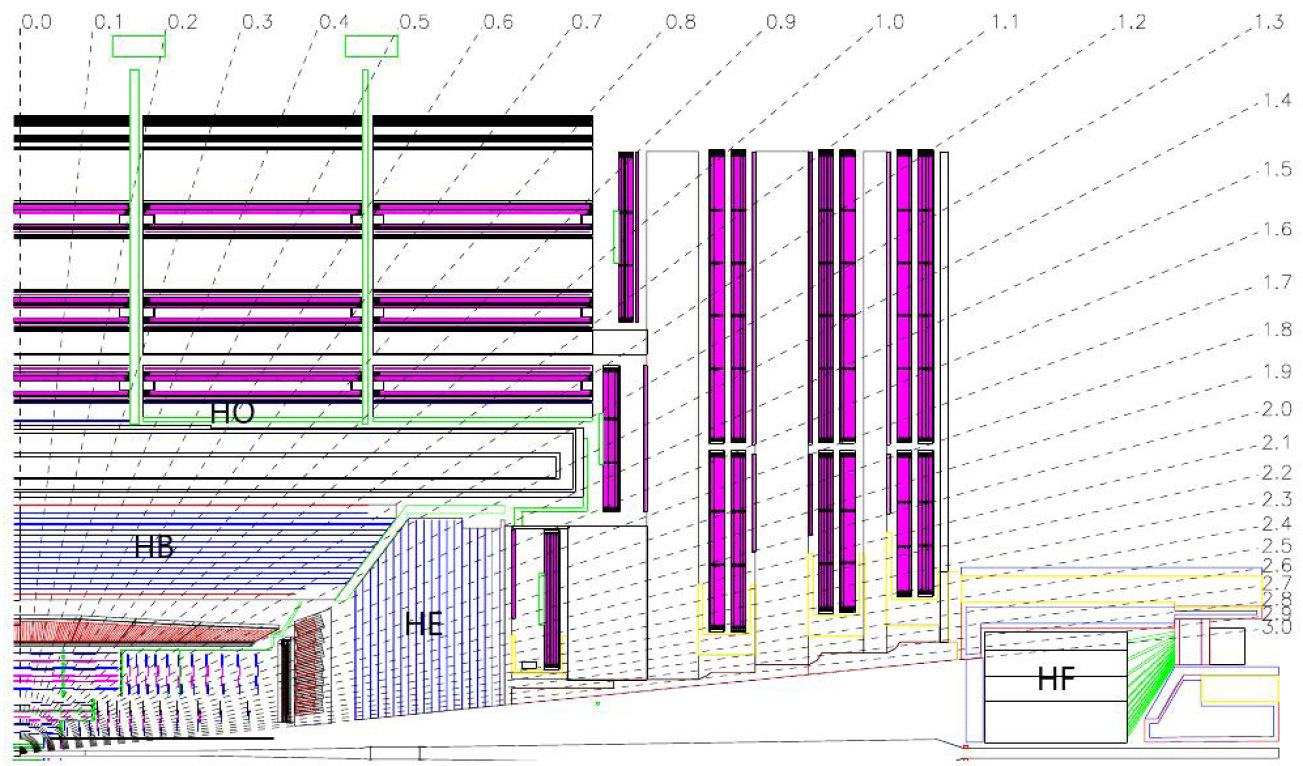
\includegraphics[width=0.8\textwidth]{\chthree/HCAL.png}
 \end{center}
 \caption{Longitudinal view of the CMS detector showing the locations of the hadron barrel (HB), endcap (HE), outer (HO) and forward (HF) calorimeters~\cite{Chatrchyan:2008zzk}.}
 \label{fig:HCALLayout}
\end{figure}

%%%%%%%%
\subsection{Muon detectors}\label{subsec:muonchambers}
%%%%%%%%

The muon system is the outermost part of the CMS detector. It is located in the steel return yoke of the solenoid, covering the pseudorapidity region $|\eta| < 2.4$. This is possible because muons are hardly affected by the large amount of material placed between the interaction point and the muon system. The coil acts as a shield from electromagnetic and hadronic particles escaping the calorimeters, and the yoke provides a magnetic field between consecutive muon stations, allowing a momentum measurement independent from the inner tracker. The muon system is designed for three major functions: robust and fast identification of muons, good resolution of momentum measurement, and integration to a fast and reliable trigger system. The gaseous detectors have been chosen since they are robust and with a relative fast response. Furthermore, the area to be covered is extremely wide and a gaseous detector system allows the reduction of cost and amount of readout channels. The muon system is thus composed of three types of gaseous detectors arranged in barrel and endcap sections, as shown in Fig.~\ref{fig:MuonSystem}: Drift Tubes (DTs), Resistive Plate Chambers (RPCs) and Cathode Strip Chambers (CSCs). The choice of different detector topologies lies essentially in the different expected particle rates. 

In the barrel region, where the neutron-induced background is small, the muon rate is low, and the 3.8-T magnetic field is uniform, DTs with standard rectangular drift cells are used covering the pseudorapidity region $|\eta| < 1.2$. A DT cell is a 4\cm wide gas tube with a positively charged, stretched wire inside. 
The barrel DT chambers are organized in five separate wheels. Each wheel is divided into 12 sectors, each covering a 30\de azimuthal angle. In each of the 12 sectors there are 4 chambers per wheel which are concentric around the beam line and separated by the iron return yoke. Each DT chamber, on average $2\unit{m}\times2.5\unit{m}$ in size, consists of 12 layers of DT cells, arranged in three groups of four. For the first 3 stations in each wheel, the middle group measures the $z$ coordinate while the two outside groups measure the $r$-$\phi$ coordinate. The fourth and outermost station does not contain the $z$-measuring planes. Each one of the 250 DT chambers has a resolution of $\approx100\mum$ in $r$-$\phi$ and up to 150\mum in $z$, and can measure the particle direction with 1\unit{mrad} accuracy.

In the two endcap regions of CMS, where the muon rates and background levels are high and the magnetic field is large and non-uniform, CSCs are used with their fast response time, fine segmentation, and radiation resistance, covering the pseudorapidity region between 0.9 and 2.4. 
Each CSC is trapezoidal shaped multiwire proportional chambers which consists of 6 gas gaps, each gap having a plane of radial cathode strips and a plane of anode wires running almost perpendicularly to the strips. The gas ionization and subsequent electron avalanche caused by a charged particle traversing each plane of a chamber produces a charge on the anode wire and an image charge on a group of cathode strips. Thus, each CSC provides a two-dimensional position measurement, where the $r$ and $\phi$ coordinates are determined by the cathode strips and the anode wires, respectively. A total amount of 540 CSCs are arranged in 4 disks per endcaps, divided in concentric rings (3 rings in the innermost station, 2 in the others). Each chamber has a spatial resolution of about 200\mm in $r$, and $75\times150\mum$ in the $r$-$\phi$ coordinate.

In addition, there is a total of 610 RPCs added in both the barrel and endcap regions to provide a fast, independent, and highly-segmented trigger over a large portion of the rapidity range ($|\eta| < 1.6$) of the muon system. They produce a fast response, with good time resolution ($\approx2\unit{ns}$) but coarser position resolution than the DTs or CSCs. RPCs are made from two high resistive plastic plates with a voltage applied and separated by a gas volume. The signal generated by the muon when passing through the gas volume is detected by readout strips mounted on top of one of the plastic plates. Six layers of RPCs are installed in the barrel muon system, two layers in each of the first two stations and one layer in each of the last two stations. One layer of RPCs is built into each of the first three stations of the endcap.

\begin{figure}[!htb]
 \begin{center}
  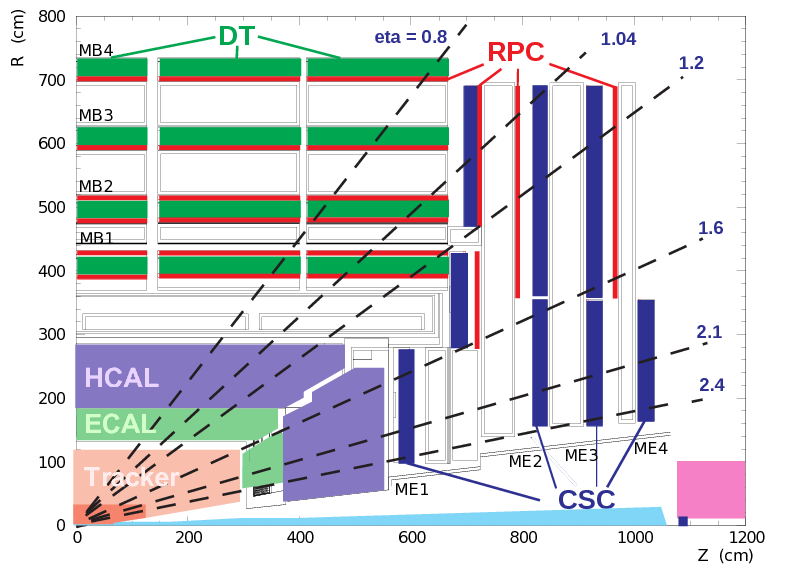
\includegraphics[width=0.8\textwidth]{\chthree/MuonSystem.png}
 \end{center}
 \caption{A longitudinal view of one quarter of the CMS experiment; the three muon detectors detector types are highlighted.}
 \label{fig:MuonSystem}
\end{figure}

%%%%%%%%
\subsection{The trigger system}\label{subsec:CMStrigger}
%%%%%%%%

The LHC provides proton-proton and heavy-ion collisions at unprecedented high luminosity and interaction rates.
Given the high segmentation of the CMS detector, about 100 million readout channels are present and this corresponds to an enormous volume of data at the detector front-ends.
At the design luminosity and collision frequency, each crossing produces approximately 1\unit{MB} of zero-suppressed data resulting in a raw data rate of about 40\unit{TB} per second. These figures are many orders of magnitude larger than the archival storage capability of $\approx1\unit{kHz}$ at data rates of $\mathcal{O}(10^2)$\unit{MB/s}.
Technical difficulties in handling, storing and processing such extremely large amounts of data impose a reduction factor on the rate of events that can be written to permanent storage. This task is performed by the trigger system, which is the baseline of the physics event selection process. The key point of the trigger system is a fast time rejection of all the ``non-interesting''
events. This can be done by exploiting event topologies common to a group of physics processes, such as the presence of one or more leptons in the event. The trigger system needs to be as inclusive as possible, in order to collect data for all the physics searches that can be performed with pp collisions, but it has also to operate within the CMS time restriction and avoid the saturation of the storage capability. The required rejection power of $\mathcal{O}(10^5)$ is too large to be achieved in a single processing step, since a high efficiency has to be maintained for the physics phenomena that CMS plans to study. For this reason, the full selection task is split into two steps. The first step (\Lone Trigger) is designed to reduce the rate of events accepted for further processing to less than 100\unit{kHz}. The second step (High-Level Trigger or ``HLT'') is designed to reduce this maximum L1 accept rate of 100\unit{kHz} to a final output rate of 1\unit{kHz}.\\

The L1 Trigger is built from custom-designed, programmable electronics and is housed partly on the detectors, partly in the underground control room located at a distance of approximately 90\unit{m} from the experimental cavern. It is designed to take a fast accept/reject decision every bunch crossing, on the basis of a rough reconstruction of the event. 
%The allowed L1 Trigger latency is 3.2 $\mu$s, therefore the processing must be pipelined in order to enable a quasi-deadtime-free operation.
The detector information used at L1 are coarsely segmented data from the calorimeters and the muon system only. Within a time budget of 3.2\mus, the system must decide if an event should be discarded or kept, and transfer this decision back to the subdetectors, which in the meantime store the high resolution data in the front-end electronics. Figure~\ref{fig:TriggerSystem} shows the L1 Trigger architecture: it has local, regional and global trigger components. 

\begin{figure}[!htb]
 \begin{center}
  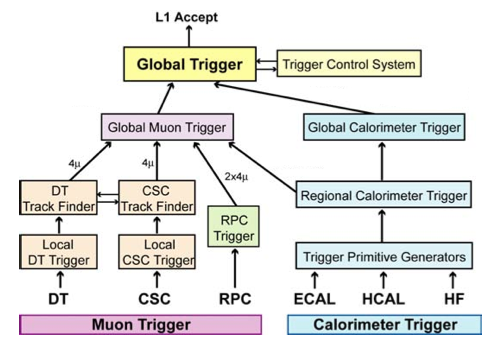
\includegraphics[width=0.7\textwidth]{\chthree/TriggerSystem.png}
 \end{center}
 \caption{Architecture of the \Lone Trigger~\cite{Chatrchyan:2008zzk}.}
 \label{fig:TriggerSystem}
\end{figure}

Trigger primitives are generated by calculating the transverse energy of a trigger tower and assigning it to the correct bunch crossing. A regional calorimeter trigger then determines regional electron, photon and jet candidates and information relevant for muon and $\tau$ lepton identification. The global calorimeter trigger provides information about the jets, the total transverse energy and the missing energy in the event and identifies the highest-energy trigger candidates.

In the muon system all three types of detectors take part in the trigger decision. The DT chambers provide track segments in the projection and hit pattern in $\eta$, while the CSCs provide three-dimensional track segments. The track finders in the DT chambers and the CSCs calculate the transverse momentum of a track segment and its location and quality. The RPCs deliver an independent measurement derived from regional hit patterns. The global muon trigger receives up to four candidates from each subsystem (DT, barrel RPC, CSC and endcap RPC) together with the isolation information from the global calorimeter trigger. The aim is to improve the efficiency and to reduce the rate by making use of the complementarity and the redundancy of the subsystems. In the end, the global muon trigger selects a maximum of four muon trigger candidates and determines their momentum, charge, position and quality.

The trigger objects extracted by the global calorimeter trigger and the global muon trigger are sent to the global trigger where the decision to accept or reject an event is taken and distributed to the subdetectors. 
%The decision is based on the results of algorithms which for example apply momentum thresholds to single objects or require object multiplicities to exceed predefined values.
The simplest triggers are in general those based on the presence of one object with an \ET or \PT above a predefined threshold (single-object triggers) and those based on the presence of two objects of the same type (di-object triggers) with either symmetric or asymmetric thresholds. Other requirements are those for multiple objects of the same or different types (``mixed'' and multiple-object triggers).
%More than 100 algorithms can be executed in parallel.
The decision is also based on the readiness of the subdetectors and the data acquisition system (DAQ), which is supervised by the Trigger Control System (TCS). The Level-1 Accept (L1A) decision is communicated to the subdetectors through the Timing, Trigger and Control (TTC) system.\\ 

If an event is accepted by the L1 trigger, the full detector information ($\approx1\unit{MB}$) is read out by the DAQ system and passed to the HLT system for further analysis. The HLT is a special part of the CMS software which runs on a farm of several thousand processors performing high-level object reconstruction and analysis.
%The HLT system is an event filter farm which runs the same software as used for offline high-level reconstruction and analysis.
Each processor works on the reconstruction of one event at a time, to get to a trigger decision within on average 100\unit{ms}. Since the time budget for one event is much larger than at the L1 trigger, more complicated algorithms, including tracking, can be executed at the HLT. Once an event is accepted, it is stored on disk and fully reconstructed offline at a later time. 

The full detector readout is available at HLT, but in order to meet the timing requirements given by the input rate from L1, events are discarded before being fully reconstructed, as soon there is enough reconstructed information to take the decision. Therefore the selection is organized in a sequence of logical steps. The \Ltwo uses the full information from calorimeters and muon detectors to reconstruct the physical objects and to reduce the event rate by roughly one order of magnitude. The data from the silicon tracker represent almost 80\% of the event size and require complex and time consuming algorithms for the reconstruction. For this reason this information is used only during the \Lthree selection.

The HLT consists of approximately 400 trigger paths. Each trigger path starts from the seed provided by the L1 trigger and it is built from reconstruction modules and filter modules. After some parts of the data are reconstructed, a filter module decides if the reconstructed objects pass the thresholds and the next step in reconstruction is started, or if the event is not accepted by the path. In the later case, the execution of the path is stopped and the following reconstruction steps and filter steps are not performed to save computation time. 
%The less computation intense reconstruction steps are done first. The reconstruction steps that take a lot of time, e.g. the tracking, are done at the end of a path for objects that have already passed the previous steps. 
If an event is not accepted by a path, it can still be accepted by a different path.
%The HLT algorithms and filters are several and dedicated to various physical searches and different operating conditions (instantaneous luminosity, centre of mass energy, ect.). 
%The HLT menu is composed of a set of trigger paths, each path addressing a specific physics object selection. The execution of a path is interrupted if the processed event does not fulfill the conditions imposed by a given filter module.

If, for some paths with low thresholds, the acceptance rate is too high, they can be prescaled to lower the rate. A prescale value of ten means, for example, that the path is executed only for every tenth event that was accepted by the L1 trigger, and, consequently, the trigger rate for that path is ten times smaller. The prescale value for one trigger path has several predefined levels, depending on the instantaneous luminosity of the LHC machine. During an LHC fill, the instantaneous luminosity decreases, and the prescale values can be changed during a CMS run to keep the global trigger rate at an optimal level.

%\section{The CMS detector simulation}
%
%For a detailed understanding on how interactions in proton-proton collisions at the LHC are observed by the CMS detector, a dedicated simulation of the whole detector and the subatomic interactions is needed [5]. Both the propagation of particles through the detector material as well as the response of the active detector components and their digital output need to be sim- ulated. The input to the detector simulation are collections of particles produced by MC event generators. The output is the digital signal from all detector components in the same format that is used for real data (RAW).
%The CMS simulation is based on the GEANT4 toolkit~\cite{Agostinelli:2002hh}. It allows modeling of the full detector geometry and the simulation of particles? propagation through magnetic fields as well as electromagnetic and hadronic interactions with the crossed material. The simulation is per- formed in two steps: the simulation step and the digitization step. In the simulation step, parti- cles are propagated through the detector allowing for interaction with detector material. Hits are produced on interaction with sensitive detector components. In the digitization step, the elec- tronic readout of these hits is simulated, taking into account resolution and detector response effects.
%
%The particles that are generated by the event generators are then propa-
%gated through the detector with the GEANT 4 [72,73] program, which simu-
%lates the detector response to these particles. Using a detailed model of the
%CMS detector including the geometries and materials, GEANT 4 generates
%the hits and particle showers that would happen in the subdetectors and sub-
%sequently simulates the response of the detector electronics to these signals.
%After the simulation by GEANT 4, the data format of a simulated event is
%the same as for the data, so that, from this point onward, the same software can
%be used for the reconstruction of data and simulation. Pileup is included in the
%samples by mixing randomly chosen minimum bias events with the simulated
%events to achieve the expected PU distribution, shown in Figure 2.4.

 
    
    



\part{Search for diboson resonances with CMS}

%\chapter{Diboson resonances as signature for new physics}
	\chapter{Diboson resonances as signature for new physics}
\label{ch:dibosonIntro}

This part of the thesis is dedicated to the description and discussion of searches for new physics in proton-proton collision data collected with the CMS experiment at LHC.
As pointed out in Chapter~\ref{ch:theory}, the remarkable compatibility of the discovered scalar resonance by the ATLAS and CMS collaborations with the SM predictions for the Higgs boson,
force physicists to deeply understand the role of naturalness in the dynamics of this particle.
Several theoretical extensions to the SM have been proposed offering a concrete realization of naturalness,
where new particles with masses in the TeV range generate loop corrections with the necessary cancellations to stabilize the Higgs boson mass.
%This means that particular attention can be payed to direct experimental manifestations of new physics represented by the production of these heavy particles.
More natural solutions can therefore be probed at the LHC through the direct discovery of these new, heavy particles in final states with SM objects with known properties.
The research described in this work follows exactly this approach and it is focused on the direct search for new massive resonances decaying to
pairs of vector bosons (WW, WZ, or ZZ) or to a vector boson and a Higgs boson (WH or ZH).
These decay modes can have large branching fractions in several BSM models. 
Popular examples include the bulk scenario of the Randall--Sundrum warped extra-dimentions model described in Section~\ref{subsec:graviton},
as well as the composite Higgs and littlest Higgs models discussed in Section~\ref{subsec:composite}.
Furthermore, the heavy vector triplet model (Section~\ref{subsec:hvt}) generalizes a large class of explicit theories that predict new heavy spin-1 vector bosons,
adopting a simplified model strategy. The two HVT models A and B are considered, which correspond, respectively, to a weakly- and a strongly-coupled theoretical option.
In this context, spin-1 resonances are studied that couple both as a vector triplet ($\PVpr = \Wpr$ and \Zpr) and as singlets (\Wpr or \Zpr), i.e. only a charged or a neutral resonance is expected at a given mass.
The properties of the above benchmark models studied in this thesis are summarized in Table~\ref{tab:models}.\\

\begin{table}[!htb]
\centering
\caption{Summary of the properties of the heavy-resonance models considered in the combination. The polarization of the produced W and Z bosons in these models is mostly longitudinal, as decays to transverse polarizations are suppressed.}
\resizebox{\textwidth}{!}{
\begin{tabular}{cccccc}
\hline
Model & Particles & Spin & Charge & Main production & Main decay \\
\hline
\multirow{3}{*}{HVT model A, $g_\mathrm{V} = 1$} & W' singlet & 1 & $\pm1$ & $\qqbar^\prime$ & $\qqbar^\prime$ \\ 
                                                                                 & Z' singlet & 1 & 0 & $\qqbar$ &  $\qqbar$\\
                                                                                 & W' and Z' triplet & 1 & $\pm1$,0 & $\qqbar^\prime$,$\qqbar$ & $\qqbar^\prime$,$\qqbar$\\
\hline
\multirow{3}{*}{HVT model B, $g_\mathrm{V} = 3$} & W' singlet & 1 & $\pm1$ & $\qqbar^\prime$ & WZ,WH \\ 
                                                                                 & Z' singlet & 1 & 0& $\qqbar$ &  WW,ZH \\
                                                                                 & W' and Z' triplet & 1 & $\pm1$,0 & $\qqbar^\prime$,$\qqbar$ & WZ,WH,WW,ZH\\
\hline
%2 / neutral / $G_{\text{RS1}}$ & subdominantly WW, ZZ & mainly $\qqbar$ and $gg$ \\
RS bulk, $\tilde{k}=0.5$ & $\rm G_{bulk}$ & 2 & 0 & $gg$ & WW, ZZ \\
\hline
\end{tabular}}
\label{tab:models}
\end{table}

The signal under investigation is a narrow resonance, referring to the assumption
that the resonance's natural width is smaller than the experimental resolution, covering a large fraction of the parameter space of the reference models considered.
%that the resonance's natural width has a negligible impact on the distribution of the resonance mass reconstructed in the detector.
This assumption allows a ``model-independent'' type of search, where the description of the resonance mass distribution can be restricted to the detector effects only and hence,
independently from the chosen benchmark model.

The semi-leptonic final states are considered, where one of the two bosons is a W decaying into a charged lepton ($\ell$) and a neutrino ($\Pgn$).
The lepton can be either a muon ($\mu$) or an electron (e), although the results include the $\PW\to\tau\Pgn$ contribution from the decay $\tau\to\ell\Pgn\bar{\Pgn}$.
However, the gain in sensitivity from $\tau$ leptons is limited by the small branching fractions involved.
The second boson in the final state decays into quarks, and can be either a vector boson V = W or Z,
or a Higgs boson. In the first case, the final state is labelled as $\ell\Pgn\qqbar$ including $\PW\to\qqbar^\prime$ and $\PZ\to\qqbar$ decays (Figures~\ref{fig:FDsignals_a},~\ref{fig:FDsignals_b} and~\ref{fig:FDsignals_c}).
For the Higgs boson, the final state is labeled as $\ell\Pgn\bbbar$ referring to the Higgs boson decay into a bottom quark-antiquark pair (Fig.~\ref{fig:FDsignals_d}).
Each quark from the V or H boson decays results in a shower of hadrons in the final state called a \textit{jet}. These particles are collected through a jet algorithm which allows to reconstruct the kinematics of the original quark.
These final states provide high sensitivity to this search as the presence of the lepton in the final state highly suppresses the QCD background, while the large branching fractions of the dominant $\PV\to\qqbarpr$ and $\PH\to\bbbar$ decay modes allow to maintain high signal cross sections.

\begin{figure}[!htb]
\centering
\subfigure[]{\label{fig:FDsignals_a}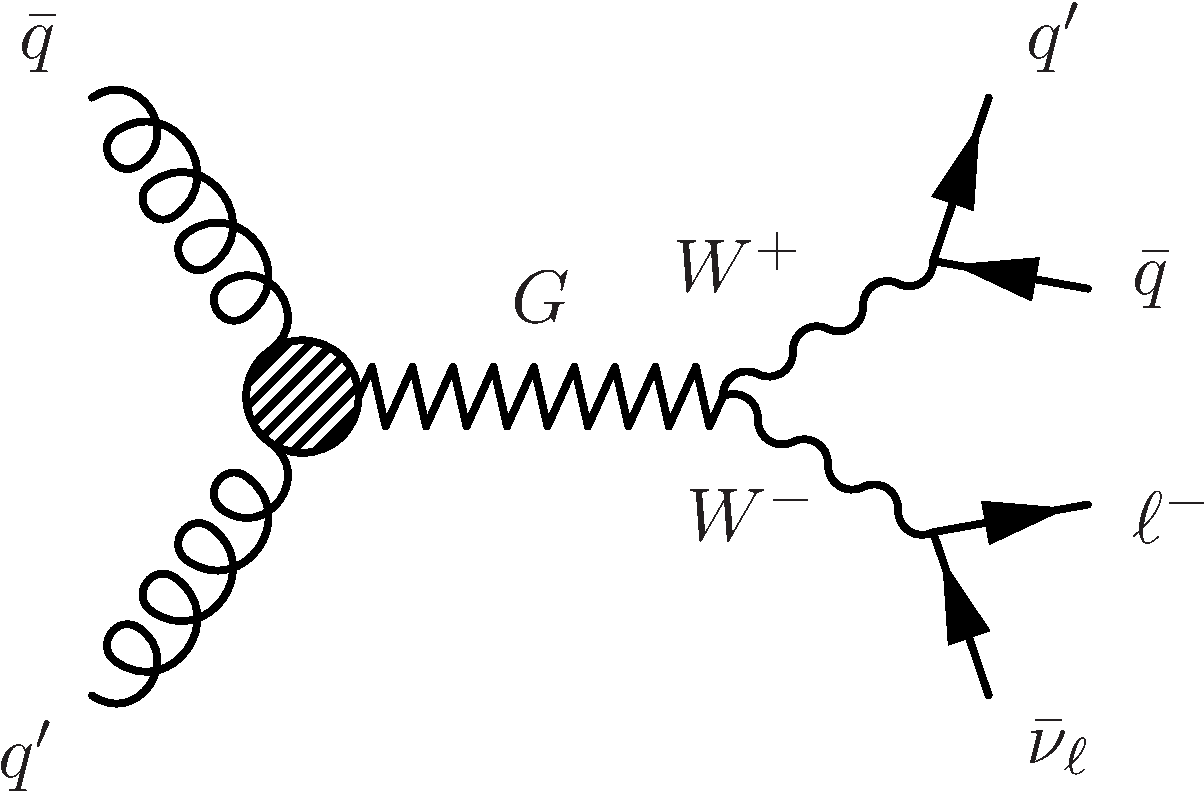
\includegraphics[width=0.3\textwidth]{\chfour/BulkGWW_LO.pdf}}\hspace{1cm}
\subfigure[]{\label{fig:FDsignals_b}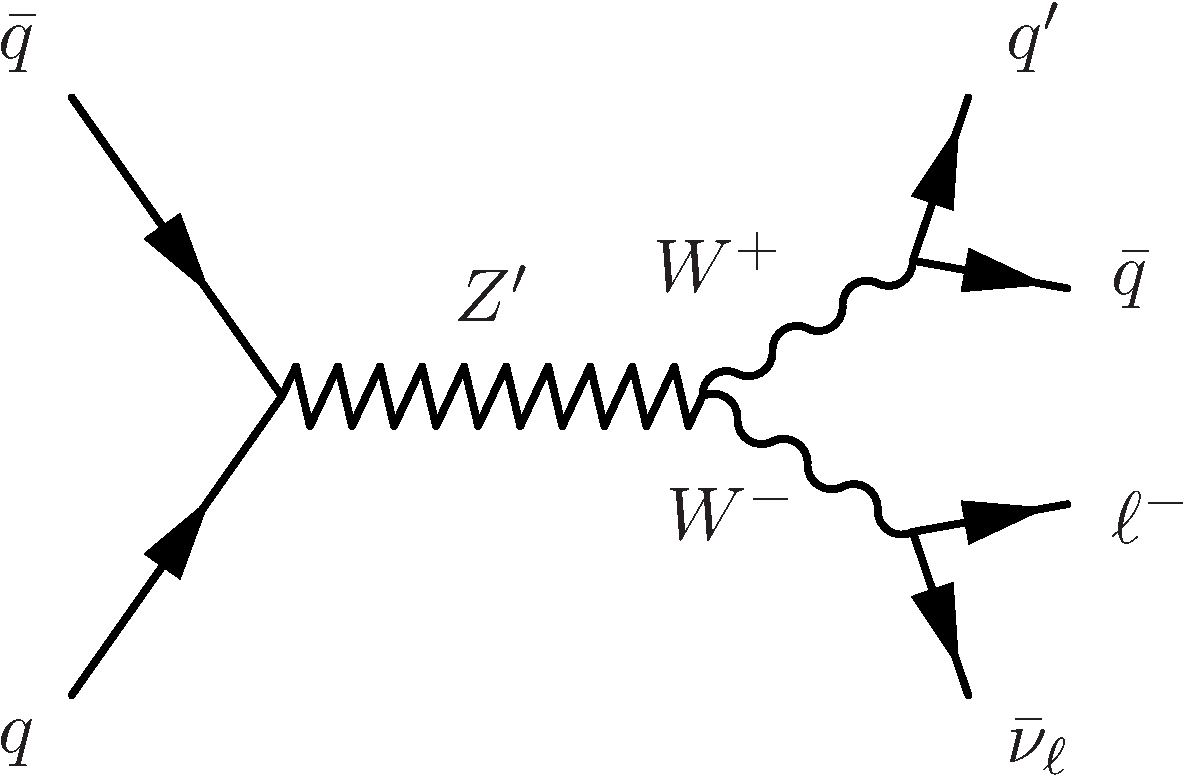
\includegraphics[width=0.3\textwidth]{\chfour/ZprimeWW_LO.pdf}}\\
\subfigure[]{\label{fig:FDsignals_c}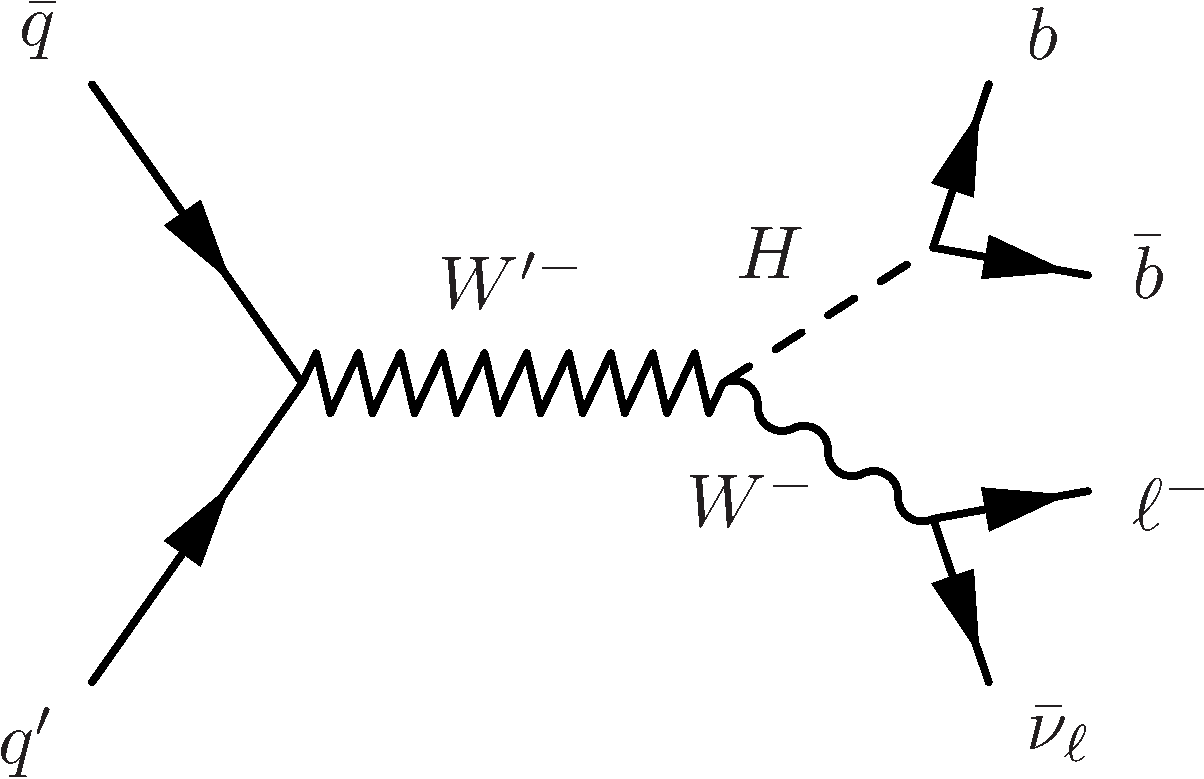
\includegraphics[width=0.3\textwidth]{\chfour/WprimeWH_LO.pdf}}\hspace{1cm}
\subfigure[]{\label{fig:FDsignals_d}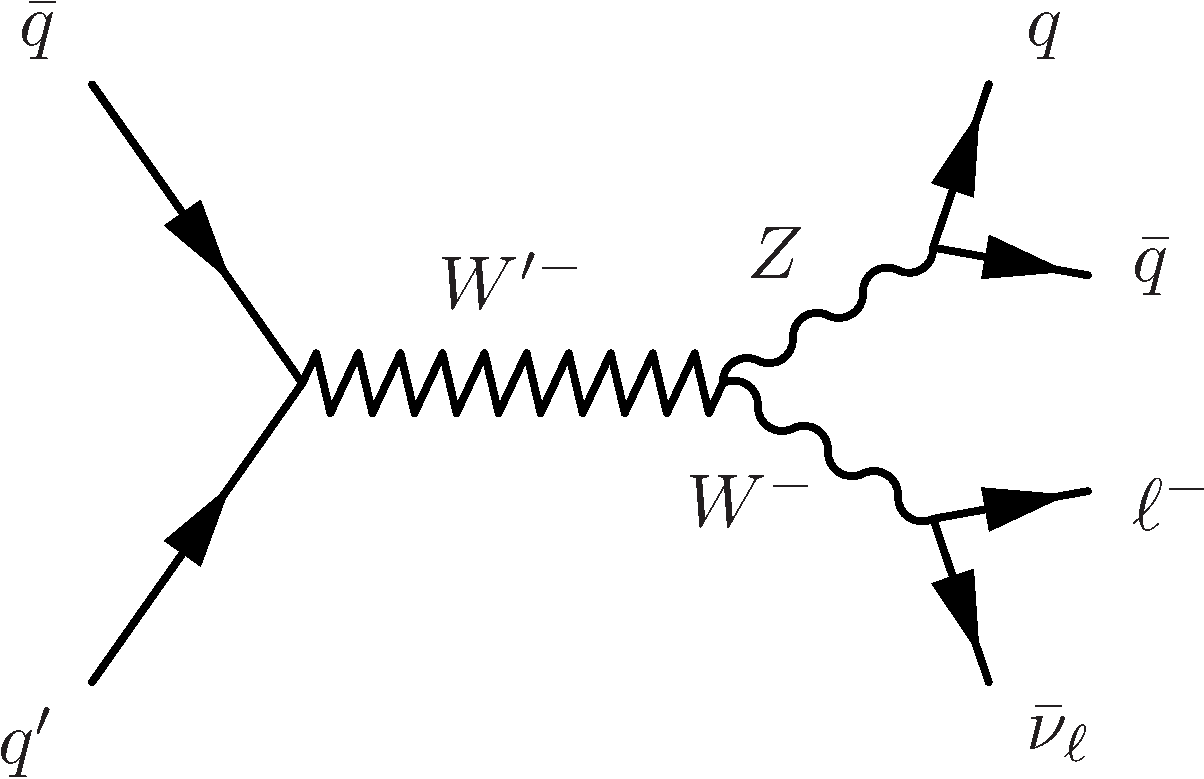
\includegraphics[width=0.3\textwidth]{\chfour/WprimeWZ_LO.pdf}}
\caption{Feynman diagrams for the production of a neutral spin-2 $G$ (a), and a neutral \Zpr (b) and charged \Wpr (c and d) spin-1 resonances.
All resonances decay to a pair of bosons (WW, WZ, or WH) with their subsequent semi-leptonic decay. Charge conjugate modes for \Wpr production and decay are implied.}
\label{fig:FDsignals}
\end{figure}

The search in the $\ell\Pgn\bbbar$ final state is based pp collision data at $\sqrt{s} = 8\TeV$ collected in 2012 and corresponding to an integrated luminosity of 19.7\fbinv.
The second analysis described in this thesis and focused on the $\ell\Pgn\qqbar$ final state is instead based on the pp collision data at $\sqrt{s} = 13\TeV$
collected in 2015 and corresponding to an integrated luminosity of 2.3\fbinv.
Although different algorithms are used for the reconstruction and identification of the hadronically decaying boson, the analysis strategy is similar in the two searches.\\

The key challenge of these analyses is the reconstruction of the highly energetic decay products.
Since the resonances under study have masses of $\approx$~TeV, their decay products, i.e. the bosons,
have on average transverse momenta of several hundred GeV or more.
As a consequence, the particles emerging from the boson decays are very collimated.
In particular, the decay products of the bosons cannot be resolved using the standard algorithms,
but are instead reconstructed as a single jet object. Dedicated techniques, so-called jet ``V tagging'' and ``H tagging'' techniques,
are applied to exploit the substructure of such jet objects, and can help resolve jet signatures of massive bosons.
In particular, the jet is tagged as coming from a V or H boson through the estimation of its invariant mass.
These techniques also help to suppress SM background, which mainly originates from the production of W bosons in association with jets (W+jets).
Further discrimination is achieved in the $\ell\Pgn\bbbar$ analysis channel exploiting the specific characteristics of jets arising from the hadronization of bottom quarks.\\

The aim is to reconstruct the full event to be able to search for a localized enhancement in the invariant mass of the WV or WH system on the top of a smoothly falling SM background distribution.
The invariant mass of the WV and WH system is determined by estimating the neutrino transverse momentum with the measured missing transverse energy in the event,
while an estimate of the neutrino longitudinal momentum is derived by imposing the constraint of the W mass on the invariant mass of the $\ell\Pgn$ system.
In the following, the diboson invariant mass will be labelled either \mlvj, or \mWV and \mWH for the $\ell\Pgn\qqbar$ and $\ell\Pgn\bbbar$ final states, respectively.
The SM background mainly comprises W+jets production, although another significant contribution is represented by the production of top quark-antiquark pairs (\ttbar).
Other minor backgrounds are represented by single top quark and SM diboson (WW, WZ or ZZ) production processes.
The mass spectrum for the dominant W+jets background is estimated from observed events with a reconstructed jet mass not compatible with the V or H hypothesis.\\ 
%This strategy partially relies on the simulation of the background processes.
%Furthermore, simulated events are used for the optimization of the analysis selection aimed at maximizing the discrimination of the signal against the background and hence the analysis sensitivity.\\

This part of the thesis is organized as follows.
Chapter~\ref{ch:dataAndSim} gives an overview of the methods used to simulate the physics processes happening in pp collisions at the LHC
together with a description of the specific simulated background and signal events used in this analysis, as well as a discussion about the data sets analyzed.
Chapter~\ref{ch:EventReconstruction} provides a detailed description of the algorithms used in CMS for the reconstruction of the event and of the physics objects expected in the lepton+jet final states under investigation.
Particular attention is given to the V and H tagging algorithms representing the key feature of this analysis and therefore, separately discussed in Chapter~\ref{ch:vtagging}.
The analysis strategy, already outlined here, is explained in details in Chapter~\ref{ch:strategy}.
This includes the final event selection and categorization optimized to enhance the analysis sensitivity,
as well as the strategy for the estimation of the expected background, the modelling of the signal and the related systematic uncertainties
which will be used as input to the statistical analysis of the diboson invariant mass distribution observed in data.
The final results are discussed in Chapters~\ref{ch:results8} and~\ref{ch:results13} for the 8 and 13\TeV data analysis, respectively. 
Eventually, these results are combined with limits derived in companion CMS searches for resonances decaying to a pair of bosons in several different final states, with data collected in both LHC Run~1 and Run~2.
%These analyses use the same V and H tagging techniques as presented here to separate the signal from the large multijet or V+jets background.
The statistical combination represent the last piece of this work and it is presented in Chapter~\ref{ch:combination}.

%\chapter{Dataset and event simulation}
	%%%%%%%%%%%%%%%%%%%%%%%%%%%%%%%
\chapter{Data sets and simulated samples}
\label{ch:dataAndSim}
%%%%%%%%%%%%%%%%%%%%%%%%%%%%%%%

The simulation of pp collisions is usually performed by means of Monte Carlo (MC) event generators, providing an accurate modelling of the event kinematics and topology.
The hard inelastic scattering has to be fully calculated: from the hard interaction between the partons inside the protons, where perturbative QCD calculations (Section~\ref{subsec:QCD}) can be used, to the formation of particle jets from the outgoing partons.
Furthermore, it is fundamental to understand the exact response of the detector to the outgoing particles produced in pp collisions. 
Consequently, the stable outgoing particles are fed to a full detector simulation that models the interaction of those particles with the detector material and the corresponding detector response.
The simulated detector data are then subject to the same reconstruction algorithms that are also used for real data.
In this chapter, MC event generators are described in detail, followed by a brief description of the CMS detector simulation.
Finally, details are given in the last section on the pp collision data sets used to perform the searches described in this thesis.

%%%%%%%%%%%%%%%%%%%%%%%%%%%%%%%
\section{Simulation of proton-proton collisions}
%%%%%%%%%%%%%%%%%%%%%%%%%%%%%%%

%%%%
\subsection{Monte Carlo event generators}
%%%%

The generation of hard inelastic pp collisions is factorized into different steps ordered by the timescale on which they happen, as illustrated in Fig.~\ref{fig:MCgenSteps}, and described in the following.\\

\begin{figure}[!htb]
\centering
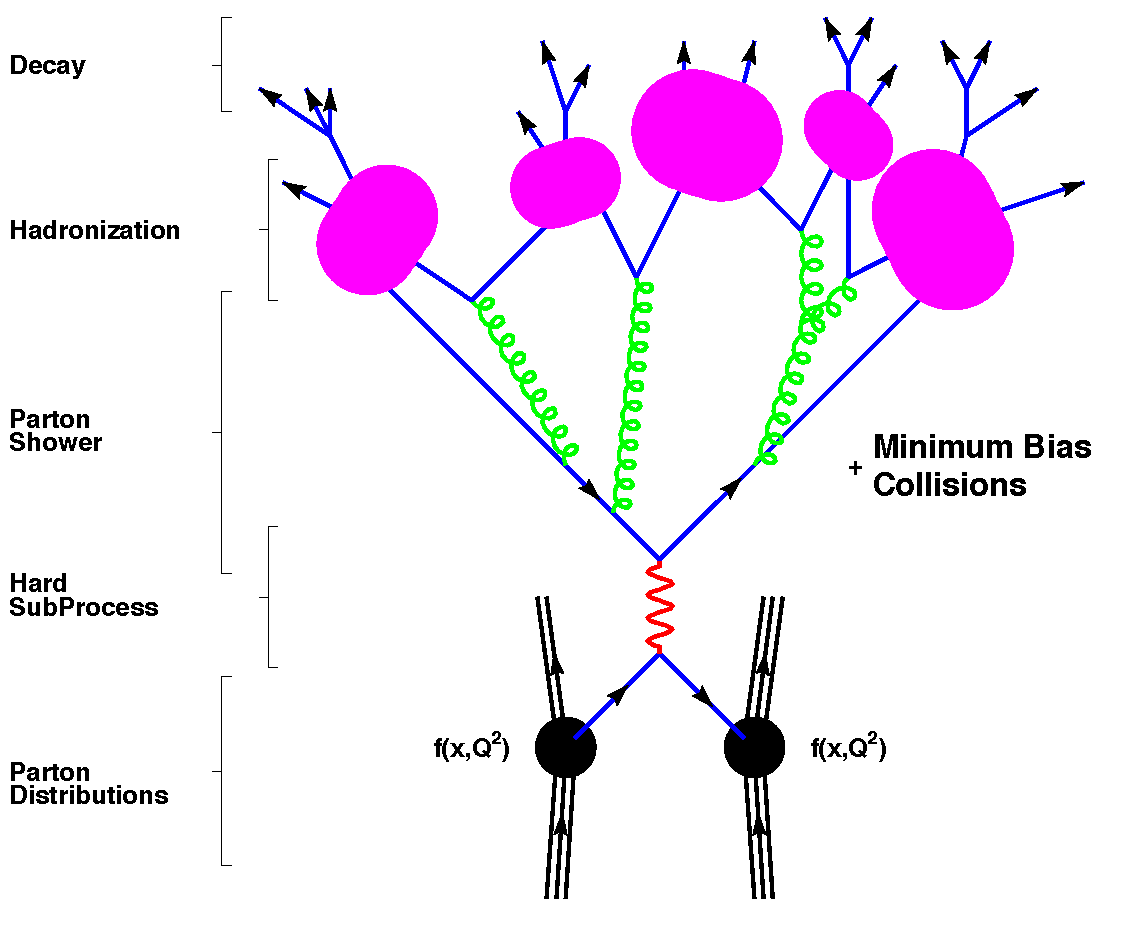
\includegraphics[width=0.8\textwidth]{\chfive/f_shg_event.pdf}
\caption{Steps of Monte Carlo event generation as described in the text evolving in time from bottom to top~\cite{Dobbs:2004qw}.}
\label{fig:MCgenSteps}
\end{figure}

The basis of theoretical event generation at the LHC is a parametrisation of the incoming partons (quarks, anti-quarks and gluons) stemming from the proton, which is given by the parton density functions (PDF).
They describe the probability to find a quark or gluon with a given proton momentum fraction $x$ in a proton of a pp collision taking place at the LHC.
In pQCD the PDFs depend on a factorization scale $\mu^2_F$ at which the proton is probed.
All interactions between quarks and gluons happening at scales below the scale $\mu^2_F$ are absorbed into the PDFs. Therefore at small $\mu^2_F$ the proton is observed basically as a combination of its
three valence quarks $uud$. At higher scales, however, it is dominated by sea quarks and gluons.

A collision between two partons, one from each side, gives the hard process of interest, which can be due to an interaction described within or beyond the standard model.
Using the incoming partons as input, the simulation of the hard process is performed by the event generator.
It produces hypothetical events with the distributions and rates predicted by theory based on the cross section formulae of the physics process of interest.
%Using the cross section formula the phase space is sampled and candidate events are defined by choosing values for the degrees of freedom from a uniformly distributed random number generator.

The cross section can be calculated by means of the so called \textit{factorization theorem}~\cite{Collins:1987pm}.
According to the theorem, the hadron itself is described by the whole particle composition interacting on a soft binding energy scale,
whereas the collisions occur between the partons on a hard energy scale with large transverse momenta.
The cross section for the process is then given by the convolution of the PDF $f_i(x,Q^2)$, integrated over the proton momentum fraction $x$, for the colliding protons (A, B) at an energy scale $Q^2$,
and the hard parton-parton cross sections $\hat{\sigma}_{ij} \to X$ for all combinations of two partons i and j:
%The cross section for two colliding protons can be seen as the convolution of the cross section $\hat{\sigma}_{ij} \rightarrow X$ for two interacting partons $i$ and $j$ inside the protons,
%with the parton distribution functions $f_1(x_1, Q^2)$, $f_2(x_2, Q^2)$ (PDF), integrated over the Bjorken variables $x_1$, $x_2$,
%defined as the fraction of the 4-momentum carried out by the two partons inside the proton during the collision

\begin{equation}
\sigma(AB \to X) = \sum_{q,g=0}^{n} \alpha_S^n(\mu_R^2)\sum_{ij}\int dx_i dx_j f_{i,A}(x_i,\mu_F^2) f_{j,B}(x_j,\mu_F^2) \cdot \hat{\sigma}^{(n)}_{ij\to X}(s;x_i,x_j,\mu_R^2,\mu_F^2).
\end{equation}

In the above equation $\alpha_S$ is the strong coupling constant (Section~\ref{subsec:QCD}), the index $n$ runs over the perturbative order and $s$ is the squared center-of-mass energy of the collision.
The tree-level process, where no emission of gluons or quarks happens, is called ``Leading Order'' (LO) and takes place when $n$ = 0.
Further orders are called ``Next-to-Leading Order'' (NLO, $n$ = 1), ``Next-to-Next-to-Leading Order'' (NNLO, $n$ = 2) and so on.

As it can be seen from the formula, the PDFs play a fundamental role in the description of the hard process, and it is very important to have several experimental tests to access their values.
In fact, perturbative QCD cannot predicts the PDFs, since they contain also the low energy (non-perturbative) information about the scattering.
As a consequence, PDF distributions are extracted from data, in deep-inelastic scattering experiments.
Most of the parametrizations of proton PDFs now used for the LHC have been extracted from the ZEUS~\cite{ZEUS:1993aa} and H1~\cite{ABT1997310} experiments in electron-proton collisions at the HERA collider and fixed target experiments.
The more recent parametrizations also take into account vector boson production and single-inclusive jet production from the Tevatron experiments, as well as LHC data.
Once measured for a certain momentum fraction $x_i$ at an energy scale $Q^2$, they can be extrapolated to another scale using the DGLAP (Dokshitzer-Gribov-Lipatov-Altarelli-Parisi) evolution equation~\cite{ALTARELLI1977298}.
The PDF sets used for the simulation of signal and background samples with $\sqrt{s} = 8\TeV$ are provided by the CTEQ/CT group~\cite{Pumplin:2002vw,Lai:2010vv}. This set especially incorporates the effects of Tevatron Run I jet production data on the gluon distribution and is therefore expected to describe the mainly gluon based LHC processes realistically. The CT sets additionally include measurements from HERA-1 data, new data on the asymmetry in the rapidity distribution of the charged lepton from W boson decay from CDF, and rapidity distributions of Z bosons from both CDF and \DZERO. The NNPDF sets~\cite{Ball:2011mu}, calculated with an approach based on neural network, are used for the 13\TeV simulations and the newest versions include LHC data as well.
An example of the most important parton distributions inside the proton is shown in Fig.~\ref{fig:pdfs}.\\

\begin{figure}[!htb]
\centering
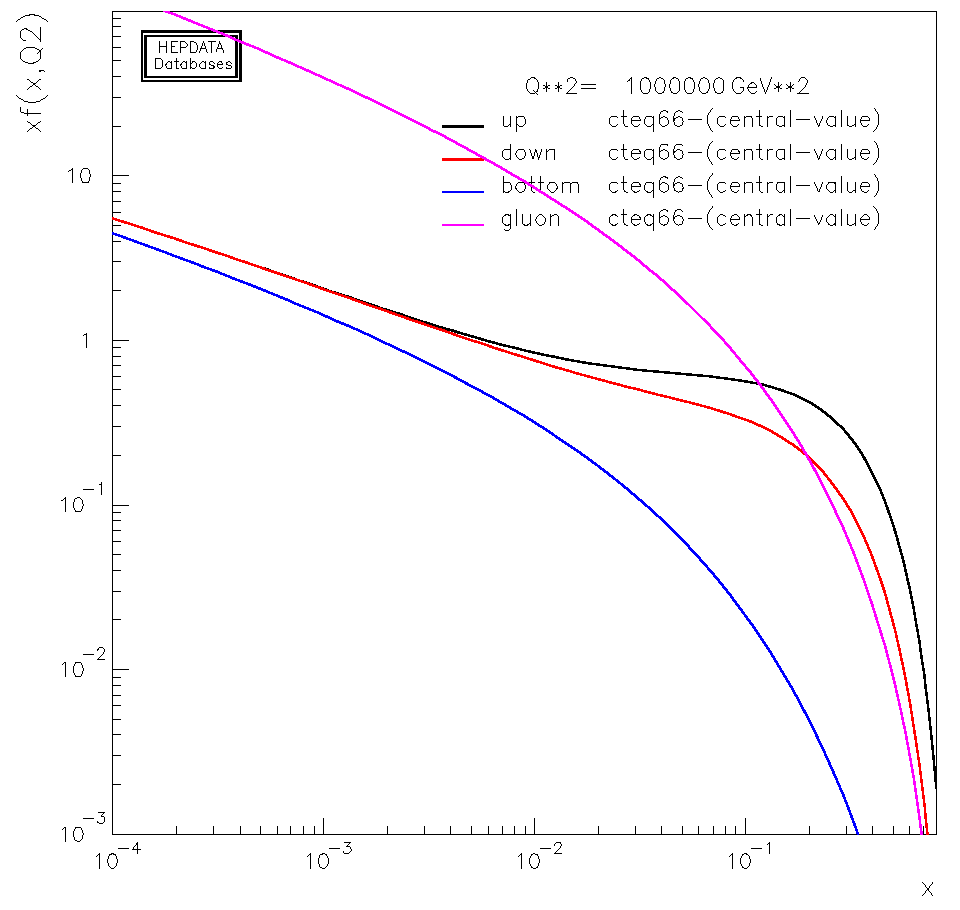
\includegraphics[width=0.45\textwidth]{\chfive/CTEQ6-pdf-set.pdf}
\caption{CTEQ6.6 central value parton distribution functions at the typical mass scale of a new diboson resonance ($Q^2 = (1000\GeV)^2$) for up, down and bottom quarks, and gluons in the proton in double-logarithmic scale.}
\label{fig:pdfs}
\end{figure}

An accurate description of the process must take into account radiative corrections to the tree-level or LO description of the process of interest.
%Indeed, a collision implies accelerated colour (and often electromagnetic) charges, and thereby bremsstrahlung can occur.
%Emissions that can be associated with the two incoming colliding partons are called Initial-State Radiation (ISR).
%Emissions that can be associated with outgoing partons are instead called Final-State Radiation (FSR).%, and can be approximated be time-like parton showers.
In particular, one has to include the effects of real and virtual higher-order corrections in perturbation theory.
This is achieved by computing the matrix element between the initial and final states as the sum of contributions with increasing powers of $\alpha_S$.
For instance, the LO contribution to the W boson production process can be calculated from the diagram in Fig.~\ref{fig:wjetsFD_LO}.
The diagrams contributing at NLO to this process and corresponding to the real and virtual radiative corrections at the first order are shown in Fig.~\ref{fig:wjetsFD_NLO}.\\

\begin{figure}[!htb]
\centering
\includegraphics[width=0.3\textwidth]{\chfive/WplusJets_LO.pdf}
\caption{(top) Feynman diagram contributing to the W boson production at leading order. The charge conjugate production mode is implied. Only the leptonic decay of the W boson is considered.}
\label{fig:wjetsFD_LO}
\end{figure}

\begin{figure}[!htb]
\centering
\subfigure[]{\label{fig:wjetsFD_NLO_a}\includegraphics[width=0.3\textwidth]{\chfive/WplusJets_NLO_1.pdf}}
\subfigure[]{\label{fig:wjetsFD_NLO_b}\includegraphics[width=0.3\textwidth]{\chfive/WplusJets_NLO_2.pdf}}\\
\subfigure[]{\label{fig:wjetsFD_NLO_c}\includegraphics[width=0.3\textwidth]{\chfive/WplusJets_NLO_3.pdf}}
\subfigure[]{\label{fig:wjetsFD_NLO_d}\includegraphics[width=0.3\textwidth]{\chfive/WplusJets_NLO_4.pdf}}
\subfigure[]{\label{fig:wjetsFD_NLO_e}\includegraphics[width=0.3\textwidth]{\chfive/WplusJets_NLO_5.pdf}}
\caption{Feynman diagrams contributing at next-to-leading order to the W boson production and corresponding to the first order real (top) and virtual (bottom) radiative corrections.
The charge conjugate production modes are implied. Only the leptonic decay of the W boson is considered.}
\label{fig:wjetsFD_NLO}
\end{figure}

Perturbative calculations in QCD are limited to processes in which the coupling constant $\alpha_S$ is small, and by the complexity of higher order calculations preventing their evaluation.
Consequently, the current generators are only able to treat a limited number of partons in the final state. 
Parton showering algorithms extend the fixed order calculations beyond these limiting factors by calculating emissions of additional partons from the in- and outgoing partons of the main interaction.
This approach in principle takes into account emissions of an unlimited number of partons, but, as opposed to full higher order calculations, does not take into account loop diagrams.
Parton showering algorithms start from the hard process allowing the partons to split (or branch) into pairs of other partons.
These again may also branch and so on, so that an event then consists of a large number of elementary particles, including quarks and gluons.
The cascade of splittings is stopped once the energy scale reaches values where the coupling constant $\alpha_S$ becomes large.

At this stage, quarks and gluons, which carry colour, cannot be considered as free anymore and recombine to form neutral hadrons, through the so called \textit{hadronization} process.
The formation of color-neutral hadrons from the colored partons is treated in phenomenological non-perturbative models.
Eventually, many short-lived resonances will be present after hadronization which are then decayed.

The showering and hadronization programs often bring along the possibility to add underlying events. The underlying event arises from the colored remains of the protons that did not take part in the hard collisions, the so-called beam remnants.
They are usually included in the hadronization process, because they might be colour-connected to the hard subprocess. The produced hadrons will however carry a very small transverse momentum and will be very forward.
The probability for colour reconnection to take place between two partons can also be adjusted based on experimental data. %---> tuning!
It is also possible that more than one parton interacts with the other proton. This phenomenon, called multiple parton interaction, and it is usually added to the description of the process.\\
%Furthermore, at the LHC there is the possibility of multiple parton interactions from the beam protons that are also added.

As last step the pileup is also accounted for.
Additional simulated inelastic pp interactions are added to the generated events to match the additional particle production due to pileup.
%The MC samples are overlaid with simulation samples reproducing the bunch train structure of the LHC beams.
%This is particularly important to take into account out-of-time pileup, i.e. additional collisions taking place before or after the actual bunch crossing of interest.
The exact number of average collisions per bunch crossing in the data is estimated by multiplying the instantaneous luminosity, continuously monitored, by the total inelastic cross section.
One can then reconstruct the distribution of the number of pileup interactions in the data for the complete data taking.
The corresponding distributions for the 2012 and 2015 data are shown in Figs.~\ref{fig:pu_mc_data_a} and~\ref{fig:pu_mc_data_c}, respectively, together with the corresponding simulated pileup scenarios.
Simulated events are then reweighted such that they match the data distribution. The description of the pileup by the simulation can be verified by counting the number of reconstructed vertices in the event as illustrated in Figs.~\ref{fig:pu_mc_data_b} and~\ref{fig:pu_mc_data_d}.\\

\begin{figure}[!htb]
\centering
\subfigure[]{\label{fig:pu_mc_data_a}\includegraphics[width=0.47\textwidth]{\chfive/PU-data-mc-8TeV.pdf}}
\subfigure[]{\label{fig:pu_mc_data_b}\includegraphics[width=0.44\textwidth]{\chfive/can_h_nVtx.pdf}}\\
\subfigure[]{\label{fig:pu_mc_data_c}\includegraphics[width=0.47\textwidth]{\chfive/PU-data-mc-13TeV.pdf}}
\subfigure[]{\label{fig:pu_mc_data_d}\includegraphics[width=0.44\textwidth]{\chfive/nPV_0.pdf}}
\caption{Distributions of the estimated average number of pileup collisions in the full data set of pp collisions recorded at $\sqrt{s} = 8\TeV$ in 2012 (a) and at $\sqrt{s} = 13\TeV$ (c), together with the corresponding simulated pileup scenarios. Also shown are the distributions of the number of reconstructed primary vertices in 8\TeV (b) and 13\TeV (d) data (black dots) and in various simulated samples after pileup reweighting, for lepton+jet events.}
\label{fig:pu_mc_data}
\end{figure}

Currently, NLO available calculations included in MC event generators cover a wide range of physics processes, starting with two particles annihilation to a maximum of five final state objects.
%Various generators are available to generate events according to a given hard process~\cite{Dobbs:2004qw}.
%Although all the orders of the perturbative development should be considered, most of the event generators only include the leading contribution to the matrix element.
A widely-used generator is \PYTHIA{}~\cite{Sjostrand:2007gs,Sjostrand:2006za}, a general purpose program which, in addition to the hard process, also takes care of the parton showering, the hadronization, and the description of the underlying event.
For the matrix element calculation, \PYTHIA{} only considers the leading order hard subprocess (diagram in Fig.~\ref{fig:wjetsFD_LO} for the W production case), and higher
order effects are added by ``evolving'' the event using the parton shower.
%The radiative corrections are not explicitely calculated but rather treated in the parton showering.
%As will be discussed in the next section, the parton showering is well suited to treat low $Q^2$ radiation.
%It however fails to accurately describe hard radiations. The consequence is that the performances of \PYTHIA{} to describe events including many hard jets in the final state are limited.
A more accurate approach is followed by \MADGRAPH{}~\cite{Alwall:2011uj} where the hard real radiative
corrections are included in the matrix element (Fig.~\ref{fig:wjetsFD_NLO}). %Diagrams with up to 5 extra partons are included.
This generator is well suited to study processes such as W or Z produced in association with hard jets.
Since it does not completely simulate the events, it needs an additional program, typically \PYTHIA{}, to perform the parton shower after the calculation of the matrix element.
It has to be noted that matrix element generators as well as shower and hadronization generators are usually treated independently: the matrix element generators compute the hard process at fixed-order and the parton shower processes the soft and collinear emissions. However, this fails to correctly represent higher order processes in which an additional parton is emitted at the hard scale because parts of this process overlap with the soft one. Combining an NLO matrix element program with a parton shower program therefore leads to double-counting of events. However, a dedicated interface between the matrix element calculation and the parton shower has been developed to correct for this effect~\cite{Hoche:2006ph}. The NLO matrix element generators, such as \POWHEG{}~\cite{Frixione:2007vw} and \MCATNLO{}~\cite{Frixione:2003ei}, take special care of the matching to the parton shower by merging soft and collinear emissions with the hard ones.
%They allow to calculate any amplitudes at NLO accuracy, and include the matching to the parton shower to produce events ready for the hadronization.
%The automatic event generator at next to leading order, \MCATNLO{}~\cite{Frixione:2003ei}, allows to calculate any amplitudes at NLO accuracy, and includes the matching to the parton shower to produce events ready for the hadronization.
%The \POWHEG{}~\cite{Frixione:2007vw} generator is another approach to calculate NLO matrix elements matched with the parton shower.
%As for \MADGRAPH{}, after the generation, the \POWHEG{} output needs to be interfaced to a chosen showering program, for example \PYTHIA{}.
%Finally, the \POWHEG{}~\cite{Frixione:2007vw} generator is a complete next to leading order (NLO) generator that considers both real and virtual corrections at the leading order.
%It is therefore limited to the radiation of one hard extra parton after what it must rely on the parton showering description.
%The use of the full NLO nevertheless provides in general an accurate estimate of the inclusive cross section. 
%In addition to event generators, there also exist cross section integrators which can be used to compute cross sections as a function of a variable of interest.
%An example is the FEWZ code [97] which allows one to make calculation at the NNLO level for exclusive production of a W or Z boson.
%cle mens: about generators
%Since the first parton radiation is already described, the interface between \POWHEG{} and the parton showering requires some special treatment.

%%%%
\subsection{CMS detector simulation}\label{subsec:fullSim}
%%%%

For a detailed understanding on how interactions in pp collisions at the LHC are observed by the CMS detector, a dedicated simulation of the whole detector is needed.
The CMS simulation is based on the \GEANTfour~\cite{Agostinelli:2002hh} toolkit, which takes as input the collections of particles produced by MC event generators.
%Both the propagation of particles through the detector material as well as the response of the active detector components and their digital output need to be simulated.
%The input to the detector simulation are collections of particles produced by MC event generators. The output is the digital signal from all detector components in the same format that is used for real data.
The program calculates the trajectory of the various particles generated during the collision, simulates their electromagnetic and hadronic interaction with the crossed material and the signal they will produce in the various subdetectors. The detector geometry is given as an input to the program, and to obtain a description as close as possible to the reality, any available information such as the existence of insensitive materials or dead channels and their position, is included. The electronic readout of the hits produced by particles is simulated, taking into account resolution and detector response effects.
The same algorithms as for real data are then used to reconstruct the various physical objects (Chapter~\ref{ch:EventReconstruction}).
%The software used by CMS, CMSSW, is a code mainly written in the C++ language which is constantly updated by the whole collaboration to integrate new knowledge on the detector (new tracker alignment or calorimeter calibration,...) or to improve the object reconstruction.

%%%%%%%%%%%%%%%%%%%%%%%%%%%%%%%
\section{Simulated samples}\label{sec:MCsamples}
%%%%%%%%%%%%%%%%%%%%%%%%%%%%%%%

\subsection{Simulation of signal processes}\label{subsec:signalMC}

For the 8\TeV data analysis, the signal hypothesis has been simulated at LO accuracy with a \Wpr boson produced via quark-antiquark annihilation and decaying into W and Higgs bosons
in the $\ell\Pgn\qqbar$ final state with q = b, c or g and $\ell$ = e, $\mu$ or $\tau$. Resonance masses in the range 0.8--2.5\TeV are considered in this analysis.
The events are generated at parton level using a model of a generic narrow spin-1 \Wpr resonance implemented with \MADGRAPH{}.
Showering and hadronization are performed using \PYTHIA{6} using the Z2* tune to describe the underlying event~\cite{Chatrchyan:2011id,Chatrchyan:2013gfi}.
It has been verified that the kinematic distributions obtained with the implementation of the generic model 
agree with those predicted by implementations of the LH, composite Higgs and HVT models in \MADGRAPH{}.
The resonance width differs in the three models, but in each case it is found to be negligible with respect to the experimental resolution.
%The full simulation of the detector has been done privately following the standard CMS procedure described in Section~\ref{subsec:fullSim}.
%This emulation has been validated comparing the private production with samples from the MC production campaign carried out centrally for the whole collaboration.

The following parameters are used to compute the cross sections: $g_\mathrm{V}$ = 3, $c_\mathrm{H} \simeq -1$, and $c_\mathrm{F} \simeq 1$
in the HVT model B (Section~\ref{subsec:hvt}) and $\cot 2 \theta$ = 2.3, cot$\theta$ = -0.20799 in the LH model, where $\theta$ is a mixing
angle parameter that determines \Wpr couplings (Section~\ref{subsec:composite}) such that $\cot 2 \theta$ and $\cot\theta$ can be directly related to $c_\mathrm{H}$ and $c_\mathrm{F}$.

The intrinsic width and cross section for both models are listed in Table~\ref{tab:gamma_xsec_LH_HVT} for the resonance masses considered.
The widths for the HVT model B are computed by means of Eq.~\ref{eqn:HVT_3},
while the cross sections were obtained using the online tools provided by the authors of the simplified model described in Section~\ref{subsec:hvt}.

\begin{table}[!htb]
\caption{
Intrinsic total widths ($\Gamma$) and cross sections for $\sqrt{s} = 8\TeV$ ($\sigma$) for the LH model and HVT model B for different masses of a resonance $\Wpr$ decaying to WH.
The $\PW\PH\to\ell\Pgn\bbbar$ branching fraction is not included in the calculation.
}
\label{tab:gamma_xsec_LH_HVT}
\begin{center}
\small
\begin{tabular}{c|cc|cc}
\multirow{2}{*}{{Resonance mass [TeV]}} & \multicolumn{2}{c}{{LH model}} & \multicolumn{2}{c}{{HVT model B}} \\
                 & $\Gamma$ [GeV] & $\sigma$ [pb] & $\Gamma$ [GeV] & $\sigma$ [pb] \\
\hline \hline
0.8 & 7.22 & 5.09$\times 10^{-1}$ & 24.1 & 3.37$\times 10^{-1}$ \\
0.9 & 8.12 & 3.03$\times 10^{-1}$ & 27.1 & 2.48$\times 10^{-1}$ \\
1.0 & 9.02 & 1.87$\times 10^{-1}$ & 30.1 & 1.71$\times 10^{-1}$ \\
1.1 & 9.92 & 1.18$\times 10^{-1}$ & 33.1 & 1.16$\times 10^{-1}$ \\
1.2 & 10.8 & 7.65$\times 10^{-2}$ & 36.1 & 8.05$\times 10^{-2}$ \\
1.3 & 11.7 & 5.06$\times 10^{-2}$ & 39.1 & 5.59$\times 10^{-2}$ \\
1.4 & 12.6 & 3.39$\times 10^{-2}$ & 42.2 & 3.88$\times 10^{-2}$ \\
1.5 & 13.5 & 2.29$\times 10^{-2}$ & 45.2 & 2.51$\times 10^{-2}$ \\
1.6 & 14.4 & 1.56$\times 10^{-2}$ & 48.2 & 1.87$\times 10^{-2}$ \\
1.7 & 15.3 & 1.08$\times 10^{-2}$ & 51.2 & 1.30$\times 10^{-2}$ \\
1.8 & 16.2 & 7.43$\times 10^{-3}$ & 54.2 & 9.03$\times 10^{-3}$ \\
1.9 & 17.1 & 5.17$\times 10^{-3}$ & 57.2 & 6.27$\times 10^{-3}$ \\
2.0 & 18.0 & 3.61$\times 10^{-3}$ & 60.2 & 4.25$\times 10^{-3}$ \\
2.1 & 19.0 & 2.53$\times 10^{-3}$ & 63.2 & 3.02$\times 10^{-3}$ \\
2.2 & 19.8 & 1.76$\times 10^{-3}$ & 66.2 & 2.10$\times 10^{-3}$ \\
2.3 & 20.8 & 1.24$\times 10^{-3}$ & 69.2 & 1.46$\times 10^{-3}$ \\
2.4 & 21.6 & 8.67$\times 10^{-4}$ & 72.2 & 1.01$\times 10^{-3}$ \\
2.5 & 22.6 & 6.07$\times 10^{-4}$ & 75.3 & 7.31$\times 10^{-4}$ 
\end{tabular}
\end{center}
\end{table}

Figure~\ref{fig:WHmodelsWidth} shows the ratio between the resonance's natural width and mass for a \Wpr in the LH and the HVT model B.
The relative width is less than 5\% for masses below 4\TeV for the following parameter values:
$0.95 < g_\mathrm{V} < 3.76$, $c_\mathrm{H}$ = -1, and $c_\mathrm{F}$ = 1;
$g_\mathrm{V} < 3.9$, $c_\mathrm{H}$ = -1, and $c_\mathrm{F}$ = 0;
or $g_\mathrm{V} < 7.8$, $c_\mathrm{H}$ =0.5, and $c_\mathrm{F}$ = 0.
The relative widths for the LH model have been computed by means of Eq.~\ref{eqn:LHvprimeWidth}, and they are less than 5\%
for values of $0.084 < |\mathrm{cot}\theta| < 1.21$. Hence, in both models the resonance's natural width can be considered to be negligible compared to the experimental resolution.\\

\begin{figure}[!htb]
\centering
\subfigure[]{\label{fig:WHmodelsWidth_a}\includegraphics[width=0.45\textwidth]{\chfive/HVT.pdf}}
\subfigure[]{\label{fig:WHmodelsWidth_b}\includegraphics[width=0.45\textwidth]{\chfive/LH.pdf}}
\caption{Ratio between the resonance's natural width and mass for a \Wpr in the LH and the HVT model B.}
\label{fig:WHmodelsWidth}
\end{figure}

For the 13\TeV data analysis, the bulk graviton model and HVT models are used as benchmark signal processes.
In these models, a resonance is simulated which decays only to pairs of vector gauge bosons in the $\ell\Pgn\qqbarpr$ final state, with $\ell$ = e, $\mu$, and $\tau$.
The vector gauge bosons are produced with a longitudinal polarization in more than 99\% of the cases.
For each resonance hypothesis, masses are considered in the range 0.6 to 4.0\TeV.
Simulated signal events are generated at LO accuracy with \amcatnlo{} with a relative resonance width of 0.1\%.

The natural width of a bulk graviton as a function of the curvature parameter $\tilde{k}$ and for different mass hypotheses is shown in Fig.~\ref{fig:bulkGwidth}.
For cases in which $\tilde{k} \leq 0.5$ the relative width of the graviton resonance ($\Gamma_\mathrm{G}/\mathrm{M}_\mathrm{G}$)
is predicted to be below 1\%. Hence, it can be neglected when compared to the detector resolution over the whole explored mass range.

\begin{figure}[!htb]
\centering
\subfigure[]{\label{fig:bulkGwidth_b}\includegraphics[width=0.45\textwidth]{\chfive/width-bulkg.pdf}}
\subfigure[]{\label{fig:bulkGwidth_a}\includegraphics[width=0.45\textwidth]{\chfive/rel-width-bulkg.pdf}}
\caption{(a) Natural width of a bulk graviton as a function of the coupling constant $\tilde{k}$ and for various mass hypotheses. (b) The same dependence is expressed as relative fraction of the signal width with respect to a reference graviton mass of 1\TeV.}
\label{fig:bulkGwidth}
\end{figure}

Figure~\ref{fig:allmodelsXsec} compare the production cross sections $\sigma(\mathrm{pp}) \to X$ of the resonance for $\sqrt{s} = 8$ and 13\TeV,
for the bulk graviton with $\tilde{k} = 0.5$, and \Wpr and \Zpr in the HVT model B, as a function of the resonance mass.
Cross sections for the bulk graviton model are computed with \MADGRAPH{} with the model used for the event generation,
while values for the HVT model B are obtained using the online tools provided by the authors of Ref.~\cite{Pappadopulo:2014qza}
using the same parameters as for the 8\TeV data analysis.

For a resonance mass of 2\TeV, the production rates at for $\sqrt{s} = 13\TeV$ are expected to increase of a factor $\approx$ 17 
for a resonance produced via gluon-gluon fusion such as the graviton; a smaller factor of $\approx$ 7 is expected instead
for resonances produced via quark-antiquark annihilation such as \Wpr and \Zpr.

\begin{figure}[!htb]
\centering
\subfigure[]{\label{fig:allmodelsXsec_a}\includegraphics[width=0.45\textwidth]{\chfive/xsec-bulkg-813.pdf}}
\subfigure[]{\label{fig:allmodelsXsec_b}\includegraphics[width=0.45\textwidth]{\chfive/xsec-hvt-813.pdf}}\\
\subfigure[]{\label{fig:allmodelsXsec_c}\includegraphics[width=0.45\textwidth]{\chfive/xsec-ratio-813.pdf}}
\caption{Comparison of the production cross sections of the resonance for $\sqrt{s} = 8$ and 13\TeV for the bulk graviton (a), and \Wpr and \Zpr in the HVT model B (b), as a function of the resonance mass.
(c) Ratio of the production cross sections for $\sqrt{s} = 8$ and 13\TeV for all models.}
\label{fig:allmodelsXsec}
\end{figure}

\subsection{Simulation of background processes}\label{subsec:bkgMC}

For the 8\TeV data analysis, the background is modelled using the \MADGRAPH{5} v1.3.30 event generator to simulate the production of W boson in association with jets at LO,
the \POWHEG{} 1.0 r1380 package to generate \ttbar and single top quark events at NLO accuracy, and \PYTHIA{6.424} for SM diboson (WW, WZ, and ZZ) production at LO.
All simulated event samples are generated using the CTEQ6L1 PDF set with $\alpha_S$ also at LO, except for the \POWHEG{} \ttbar sample,
for which the CT10 NNLO PDF set is used.
All the samples are then processed further by \PYTHIA{6}, using the Z2* tune for simulation of parton showering and subsequent hadronization,
and for simulation of the underlying event. All simulated background samples are normalized to the integrated luminosity of the recorded data, using inclusive cross sections determined at NLO,
or NNLO when available, calculated with the cross section integrators \MCFM{}~\cite{Campbell:2003hd,Campbell:2011bn,Campbell:2012uf,Campbell:2004ch}
and \textsc{fewz}~\cite{Li:2012wna}, except for the \ttbar sample, for which \textsc{top++}~\cite{Czakon:2011xx} is used.
The NNLO cross section for the W+jets process is obtained by rescaling the LO value given by the generator to the NNLO cross section
derived from the inclusive production by means of a flat $k$-factor = NNLO/LO = 1.3.
The simulated samples used in the 8\TeV data analysis described in this work are listed in Table~\ref{tab:bkgMC8TeV} together with the corresponding cross sections.\\

\begin{table}[!htb]
   \centering
   \caption{Summary of the MC generated samples for background processes used for the 8\TeV data analysis. The cross sections used to normalize the samples are also indicated.}
   \begin{tabular}{l|c|c|c}
   Process & Cross section (pb) & Generator & PDF set\\ 
   \hline
   \hline
   W+jets, $\PW\to\ell\Pgn$, $\pt^W > 180\GeV$ & 29.0 (NNLO) & \MADGRAPH{} & CTEQ6L1\\
   \hline
   \ttbar (inclusive) & 252.9 (NNLO+NNLL) & \POWHEG{} & CT10\\
   \hline
   single t quark (t-channel, inclusive) & 54.9 (NNLO) & \POWHEG{} & CTEQ6L1\\
   single $\bar{\mathrm{t}}$ quark (t-channel, inclusive) & 29.7 (NNLO) & \POWHEG{} & CTEQ6L1\\     
   single t quark (tW-channel, inclusive) & 11.2 (NNLO) & \POWHEG{} & CTEQ6L1\\
   single $\bar{\mathrm{t}}$ quark (tW-channel, inclusive) & 11.2 (NNLO) & \POWHEG{} & CTEQ6L1\\
   single t quark (s-channel, inclusive) & 3.8 (NNLO) & \POWHEG{} & CTEQ6L1\\
   single $\bar{\mathrm{t}}$ quark (s-channel, inclusive) & 1.8 (NNLO) & \POWHEG{} & CTEQ6L1\\
   \hline
   WW (inclusive) & 54.8 (NLO) & \PYTHIA{6} & CTEQ6L1\\ 
   WZ (inclusive) & 33.2 (NLO) & \PYTHIA{6} & CTEQ6L1\\ 
   ZZ (inclusive) & 8.1 (NLO) & \PYTHIA{6} & CTEQ6L1\\ 
   \end{tabular}
   \label{tab:bkgMC8TeV}
\end{table}
%W+jets generated at LO --> xsec from the generator rescaled to the one at NNLO calculated with FEWZ: NNLO = LO * k-factor, k-factor = NNLO/LO
%https://twiki.cern.ch/twiki/bin/view/CMS/StandardModelCrossSectionsat8TeV
%https://twiki.cern.ch/twiki/bin/viewauth/CMS/StandardModelCrossSectionsat8TeVInclusive
%https://twiki.cern.ch/twiki/bin/viewauth/CMS/SingleTopSigma
%https://twiki.cern.ch/twiki/bin/view/LHCPhysics/SingleTopRefXsec
%https://twiki.cern.ch/twiki/bin/view/LHCPhysics/TtbarNNLO#Top_quark_pair_cross_sections_at

For the 13\TeV analysis, the W+jets SM process is simulated with \amcatnlo{} at LO accuracy.
The \ttbar, single top quark and diboson events are generated with both \POWHEG{} and \amcatnlo{} at NLO accuracy.
Parton showering and hadronization are implemented through \PYTHIA{8} using the CUETP8M1 tune~\cite{Skands:2014pea,Khachatryan:2015pea}.
The NNPDF 3.0 PDFs with $\alpha_S$ at NLO, are used for all simulated samples. 
The simulated background is normalized using inclusive cross sections calculated at NLO, or NNLO order in QCD where available, using \MCFM{} and \textsc{fewz},
except for the \ttbar sample, for which \textsc{top++}~\cite{Czakon:2011xx} is used.
A $k$-factor = 1.21 is used to rescale the W+jets simulation to the NNLO cross section.
%The NNLO cross section for the W+jets process is obtained by rescaling the LO value given by the generator to the NNLO cross section derived from the inclusive production by means of a flat $k$-factor = NNLO/LO = 1.21.

The simulated samples used in the 13\TeV data analysis described in this work are listed in Table~\ref{tab:bkgMC13TeV} together with the corresponding cross sections.

\begin{table}[!htb]
   \centering
   \caption{Summary of the MC generated samples for background processes used for the 13\TeV data analysis. The cross sections used to normalize the simulated events are also indicated. The NNPDF 3.0 PDFs are used for all simulated samples}
 \resizebox{\textwidth}{!}{
   \begin{tabular}{l|c|c}
   Process & Cross section (pb) & Generator\\ 
   \hline
   \hline
   W+jets, $\PW\to\ell\Pgn$, $100 < \HT < 200\GeV$ & 1627.5 (NNLO) & \amcatnlo{}\\
   W+jets, $\PW\to\ell\Pgn$, $200 < \HT < 400\GeV$ & 435.2 (NNLO) & \amcatnlo{}\\
   W+jets, $\PW\to\ell\Pgn$, $400 < \HT < 600\GeV$ & 59.2 (NNLO) & \amcatnlo{}\\
   W+jets, $\PW\to\ell\Pgn$, $600 < \HT < 800\GeV$ & 14.6 (NNLO) & \amcatnlo{}\\
   W+jets, $\PW\to\ell\Pgn$, $800 < \HT < 1200\GeV$ & 6.7 (NNLO) & \amcatnlo{}\\
   W+jets, $\PW\to\ell\Pgn$, $1200 < \HT < 2500\GeV$ & 1.6 (NNLO) & \amcatnlo{}\\
   W+jets, $\PW\to\ell\Pgn$, $\HT > 2500\GeV$ & 0.04 (NNLO) & \amcatnlo{}\\ 
   \hline 
   \ttbar (inclusive) & 831.8 (NNLO+NNLL) & \POWHEG{}\\
   \hline   
   single t quark (t-channel), $\PW\to\ell\Pgn$ & 44.5 (NNLO) & \POWHEG{}\\
   single $\bar{\mathrm{t}}$ quark (t-channel), $\PW\to\ell\Pgn$ &  26.5 (NNLO) & \POWHEG{}\\       
   single t quark (tW-channel, inclusive) & 35.9 (NNLO) & \POWHEG{}\\
   single $\bar{\mathrm{t}}$ quark (tW-channel, inclusive) & 35.9 (NNLO) & \POWHEG{}\\   
   single t+$\bar{t}$ quark (s-channel), $\PW\to\ell\Pgn$ & 3.7 (NNLO) & \amcatnlo{}\\   
   \hline
   $\PW\PW\to\ell\Pgn\qqbar^\prime$ & 50.0 (NNLO) & \POWHEG{}\\ 
   $\PW\PZ\to\ell\Pgn\qqbar$ & 10.7 (NLO) & \amcatnlo{}\\ 
   $\PZ\PZ\to\ell\ell\qqbar$ & 3.22 (NLO) & \amcatnlo{}\\ 
   \end{tabular}}
   \label{tab:bkgMC13TeV}
\end{table}
%https://twiki.cern.ch/twiki/bin/viewauth/CMS/ExoDiBosonResonancesRun2#Backgrounds_AN3
%https://twiki.cern.ch/twiki/bin/viewauth/CMS/SummaryTable1G25ns#Diboson
%https://twiki.cern.ch/twiki/bin/viewauth/CMS/SummaryTable1G25ns#W_jets
%https://twiki.cern.ch/twiki/bin/viewauth/CMS/SingleTopSigma
%https://twiki.cern.ch/twiki/bin/view/LHCPhysics/TtbarNNLO
%sample generati con madgraph sono leading order. Per W+jets madgraph puo' generare fino a 4 jets at LO (--> in pratica significa che non considera i diagrammi virtuali)
%madgraph_amc@NLO genera a NLO con matching tra pythia e i matrix element di madgraph
%powheg e' come madgraph.
%pythia non riesce a generare bene eventi con alta multiplicita' di jets.
%i calcolatori di cross sections calcolano le xsec inclusive con alta precision a ~tutti gli ordini. madgraph anche puo' calcolare la xsec ma con meno precisione quindi poi l'incertezza e' maggiore.

%%%%%%%%%%%%%%%%%%%%%%%%%%%%%%%%
\section{Data sets}\label{sec:data set}
%%%%%%%%%%%%%%%%%%%%%%%%%%%%%%%

Two independent data sets are analyzed in this work to search for diboson resonances decaying to two different final states.\\

The analysis focused on the $\ell\Pgn\bbbar$ final state is performed with the complete set of data recorded in 2012 by the CMS detector
and corresponding to an integrated luminosity of 19.7\fbinv of pp collisions at $\sqrt{s} = 8\TeV$.\\
%The recorded events are divided into 4 run periods (runs A, B, C, D).\\

The second analysis described in this work in focused on the $\ell\Pgn\qqbarpr$ final state and it is performed with only the largest part of the full set of data recorded in 2015 by the CMS detector
corresponding to an integrated luminosity of 2.3\fbinv of pp collisions at $\sqrt{s} = 13\TeV$.
During 2015, there have been three running periods labeled from B to D. In fact, after a short period of 50\unit{ns} operation (period B), the machine collected data with a bunch spacing of 25\unit{ns} (period C and D).
However, since the first two periods only add a tiny contribution to the total integrated luminosity of 2015 collisions, the analysis is based on period D only, corresponding to the largest data set.\\

All events that are accepted by a specific set of high level triggers enter one specific data set, so that the choice of a trigger for the analysis defines which data set has to be used.
As discussed in the next chapter (Sections~\ref{subsec:mutrigger} and~\ref{subsec:eletrigger}), events are collected with a trigger requiring either one muon or one electron passing given \pt and $\eta$ selections.
Hence, the data sets used in these analyses are the so called ``SingleMuon'' and "SingleElectron" primary data sets listed in Table~\ref{tab:data set}.

Even though run periods of stable LHC collisions are chosen for the analyses, not all runs can be used.
This analysis requires the whole detector to be functional since the objects employed are reconstructed from all parts of the detector as described in the next chapter.
Therefore, only data-taking runs and luminosity blocks during which the detector was in a state sufficiently good for further analysis are used.

\begin{table}[!htb]
\caption{Data sets used in this analysis.}
\label{tab:data set}
\begin{center}
\begin{tabular}{c|c|cccc}
$\sqrt{s}$ & Year & Data set & Run period & Run range & $\mathcal{L}$~[pb]$^{-1}$]\\
\hline
\hline
\multirow{10}{*}{8\TeV} & \multirow{10}{*}{2012} & \multirow{5}{*}{SingleMuon} & A & 190456--193621 & 889.362 \\
& & & B & 193833--196531 & 4424    \\
& & & C & 198022--203742 & 7144    \\
& & & D & 203777--208686 & 7307    \\
\cline{4-6}
& & & Total & 190456--208686 & 19764   \\
\cline{3-6}
& & \multirow{5}{*}{SingleElectron} & A & 190456--193621 & 889.362 \\
& & & B & 193833--196531 & 4422    \\
& & & C & 198022--203742 & 7080    \\
& & & D & 203777--208686 & 7314    \\
\cline{4-6}
& & & Total & 190456--208686 & 19705   \\
\hline
\hline
\multirow{2}{*}{13\TeV} & \multirow{2}{*}{2015} & SingleMuon & D & 256630--260627 & 2320 \\
\cline{3-6}
 & & SingleElectron & D & 256630--260627 & 2320 \\
\end{tabular}
\end{center}
\end{table}
	
%\chapter{Object and event reconstruction}
	\chapter{Object and event reconstruction}
\label{ch:EventReconstruction}

\section{Tracks and vertices}
\section{Electrons}
\section{Muons}
\section{Jets}
\subsection{Identification of b jets}
\section{Missing transverse energy}
\section{W$\rightarrow\ell\Pgn$ reconstruction}


%\chapter{Boosted H->bb and W/Z->qq identification with jet substructure}
	\chapter{Identification of highly boosted W/Z$\rightarrow$\qqbarpr and H$\rightarrow$\bbbar}
\label{ch:vtagging}

\FIXME{Assume that I already introduced jet clustering algorithms in Section~\ref{sec:jets}. And I already introduce the signal topology in Section~\ref{ch:dibosonIntro}.}

Large-cone jets (see Section~\ref{sec:jets}), also referred to as ``fat jets'', are used to reconstruct the W jet, Z jet, and H jet candidates resulting after the hadronization of the two quarks from the decay of highly boosted W, Z, and Higgs boson, respectively. To discriminate against multijet backgrounds, the analyses exploit both the reconstructed jet mass, which is required to be close to the boson mass, and the jet substructure arising from the two jet cores that correspond to the two high-\pt decay quarks.\\

The techniques to identify jets arising from the merged decay products of a single V or Higgs boson is referred to as ``V tagging" or ``H tagging", respectively. It employes novel jet substructure algorithms, which are described in Section~\ref{sec:jetsubalgo}. The features of the V tagging algorithm are described in Section~\ref{sec:vtagging} and its performance in both data and simulation are discussed. 
%Discrepancies between data and simulation in the jet substructure observables used to identify the signal jets are studied through a measurement in a top quark enriched sample of data, as discussed in Section~\ref{sec:vtagging}.
Finally, in Section~\ref{sec:htagging}, a procedure tuned to the specific properties of the Higgs boson decay into a bottom quark-antiquark pair is presented.

%%%%%%%%%%%%%%%%%%%%%%%%%%%%%%%%%%%%%%%%%%%%%%%%%%%%%%%%%%%%%%%%%%%%%%%%%%%
\section{Jet substructure observables}
\label{sec:jetsubalgo}
%%%%%%%%%%%%%%%%%%%%%%%%%%%%%%%%%%%%%%%%%%%%%%%%%%%%%%%%%%%%%%%%%%%%%%%%%%%

\subsection{Pruned jet mass}
\label{subsec:pruning}

As the mass of the V or H boson is larger than the mass of a typical QCD jet, the jet mass is the primary observable that distinguishes a W jet from a QCD jet. The bulk of the W jet mass arises from the kinematics of the two jet cores that correspond to the two decay quarks. In contrast, the QCD jet mass arises mostly from large-angle and soft gluon radiation.
As a first step in exploring potential substructure, the jet constituents are subjected to a jet grooming algorithm that improves the resolution in the jet mass and reduces the effect of pileup~\cite{Chatrchyan:2013vbb,Khachatryan:2014vla}. The goal of jet grooming is to recluster the jet constituents, while applying additional requirements that eliminate soft, large-angle QCD radiation. This procedure shifts the jet mass of QCD jets to smaller values, while maintaining the mass for signal jets close to the boson mass. Furthermore, soft contributions from the underlying event and pileup, usually present in all jets, are removed.
Different jet grooming algorithms have been explored at CMS and their performance on jets in multijet processes has been studied in detail~\cite{Chatrchyan:2013vbb,Khachatryan:2014vla}. In this analysis, the \emph{jet pruning} algorithm~\cite{jetpruning1,Ellis:2009me} is used, as it provides the best discrimination against QCD background as discussed in Ref.~\cite{Chatrchyan:2013vbb,Khachatryan:2014vla}.

Jet pruning reclusters each large-cone jet starting from all its original constituents, through the implementation of the CA algorithm, but applying two additional conditions beyond those given in \FIXME{refer to the general jet clustering equation}. In particular, the softer of the two particles $i$ and $j$ to be merged is removed when the following conditions are met:

\begin{equation}
z_{ij} \equiv \frac{\mathrm{min}(p_{Ti} + p_{Tj})}{p_{Ti} + p_{Tj}} < z_{cut}\:\:,
\quad\quad\quad\quad
\Delta R_{ij} > D_{cut} \equiv \alpha\frac{m_j}{p_T}
\end{equation}

where $m_j$ and $p_T$ are the mass and transverse momentum of the originally-clustered jet, and $z_{cut}$ and $\alpha$ are parameters of the algorithm, chosen to be 0.1 and 0.5, respectively. In this particular choice of parameters, the algorithm removes the largest number of jet constituents, and can therefore be regarded as the most aggressive jet grooming technique. The resulting jet is the \emph{pruned jet}. The pruned jet mass, \mJ, is computed from the sum of the four-momenta of the constituents that survive the pruning; it is then corrected by the same factor used to correct the jet \pt (see Section~\ref{sec:jets}).
Figure~\ref{fig:mass_pr_a} illustrates the effect of pruning on AK8 jets: the \mJ spectrum of the W jet candidate from the decay of highly boosted and longitudinally polarized W bosons is shown together with the distribution in \mJ for the simulated background of W+jets. Dashed and solid lines correspond to the distributions before and after the application of the pruning algorithm, respectively. Fully merged jets reconstructed from the W boson decay generate a distinctive peak around the W boson mass, which is narrowed by the pruning, while background jets acquire a smaller mass on average, enhancing the discrimination. Figure~\ref{fig:mass_pr_b} compares the distributions in \mJ for W, Z and H jet candidates from the decay of highly boosted W, Z and Higgs bosons, respectively. The distribution in \mJ for the W+jets background is also shown. Not-full-merged signal jets give rise to a peak at low masses. 
%The \mJ distributions for W jets and QCD jets are shown in Fig.~\ref{fig:mass_pr} at generator level and reconstruction level with pileup. Comparing the generator level predictions for the \mJ of W jets with those at detector level with pileup, the widening of the peak due to detector resolution can be observed.

\begin{figure}[!htb]
\centering     %%% not \center
\subfigure[]{\label{fig:mass_pr_a}\includegraphics[width=0.45\textwidth]{\chseven/pruned-jet-mass.pdf}}
\subfigure[]{\label{fig:mass_pr_b}\includegraphics[width=0.45\textwidth]{\chseven/pruned-jet-mass-allsignals.pdf}}
\caption{(a) Distribution in pruned jet mass \mJ for simulated events of highly boosted W bosons and inclusive QCD jets expected in the W+jet topology. The ungroomed jet mass is shown as dotted lines to illustrate the effect of pruning. MG denotes the MADGRAPH generator. (b) Comparison of the distributions in \mJ for simulated events of highly boosted V and Higgs bosons.}
\label{fig:mass_pr}
\end{figure}
 
%In considering the kinematics of the substructure, two variables, $z$ and $\theta$, are particularly useful. For a recombination 1,2 $\rightarrow$ p, they are defined as:
%\begin{equation}
%z \equiv \mathrm{min}(p_{T1} + p_{T2})/p_{Tp}\:\:,
%\quad\quad\quad\quad
%\theta \equiv \Delta R_{12}
%\end{equation}
%To identify heavy particle decays reconstructed in a single jet, the interest is in recombinations that occur at large $\theta$, typically the final recombination. In general, small-$\theta$ recombinations are likely to represent the QCD showering of the decay products. Similarly, small-$z$, or soft, recombinations are typical for a QCD shower. Even the large-angle, but small-$z$, recombinations that can appear in jets from a heavy particle decay will be unlikely to yield an accurate representation of the decay: if a heavy particle decays such that one decay product has a much lower \pt relative to the others, the parent particle is unlikely to be accurately reconstructed.

%from JME-16-003: The softdrop algorithm is primarily aimed at separating W-jets from q/g-jets and does not fully reject contributions from underlying event and pileup. Therefore, a jet shape aware pileup suppressing algorithm needs to be applied in addition. We study softdrop in combination with the PUPPI algorithm 
%The pairwise merging scheme of recombination algorithms naturally gives substructure to a jet, which provides kinematic handles to determine whether the jet was produced by QCD alone or a heavy particle decay plus QCD.

\subsection{N-subjettiness}
\label{subsec:nsubj}

In addition to the pruned jet mass, additional information about the jet shape is used to discriminate the signal against jets from gluon and single-quark hadronization. This information can be obtained from the quantity called \emph{N-subjettiness}~\cite{Thaler:2010tr}. It takes advantage of the multi-body kinematics in the decay pattern of boosted hadronic objects, and it can be used to effectively ``count'' the number of subjets in a given jet. 

The N-subjettiness is a generalized jet shape observable which defines a measure, $\tau_N$, for a jet to have $N$ subjets. The constituents of the jet before the pruning procedure are reclustered using the $k_T$ algorithm (see Section~\ref{sec:jets}), until $N$ joint objects (subjets) remain in the iterative combination procedure of the algorithm. The observable $\tau_N$ is then defined as

\begin{equation}
\tau_N = \frac{1}{d_0} \sum_{k} p_{T,k}~\mathrm{min} \{\Delta R_{1,k},\Delta R_{2,k},\cdots,\Delta R_{N,k}\}
\end{equation}

where $k$ runs over the constituents of the jet, and the distances $\Delta R_{n,k}$ are calculated relative to the axis of the $n$th subjet. %We use a one step optimization of the exclusive kT axes to define the subjet axes.
The normalization factor $d_0$ is taken as

\begin{equation}
d_0 = \sum_{k} p_{T,k} R_{0}
\end{equation}

where $R_0$ is the characteristic jet radius used in the original jet clustering algorithm. The subjet axes are obtained by running the exclusive $k_T$ algorithm~\cite{Ellis:1993tq}, and reversing the last $N$ clustering steps. The variable $\tau_N$ quantifies to what degree the jet can be regarded as a jet composed of $N$ subjets. Jets with $\tau_N \approx 0$ have all their radiation aligned with the candidate subjet directions and therefore have $N$ (or fewer) subjets. Jets with $\tau_N \gg 0$ have a large fraction of their energy distributed away from the candidate subjet directions and therefore have at least $N+1$ subjets.
%The \tau_N$ observable has a small value if the jet is consistent with having N or fewer subjets, as almost every jet constituent will be close in ?R to its own true subjet.
%For discrimination between W jets with two subjets and QCD jets consistent with a single subjet, the ratio $\tau_2/\tau_1$ is particularly useful as it tends to smaller values for W jets.
The ratio between 2-subjettiness and 1-subjettiness, $\tau_{21} = \tau_{2}/\tau_{1}$, is found to be a powerful discriminant between jets originating from hadronic V decays and from gluon and single-quark hadronization. Jets from W or Z decays in signal events are characterized by lower values of $\tau_{21}$ relative to QCD background.
%We find that ?2/?1 is an effective discriminating variable to identify two-prong objects like boosted W, Z, and Higgs bosons.
Figure~\ref{fig:tau21} shows the $N$-subjettiness ratio $\tau_{21}$ distribution for W jets and QCD jets after requiring 60 $< \mJ <$ 100\GeV, and demonstrates its discrimination power after the pruned jet mass selection. %The distributions at detector level with pileup are shifted significantly compared to the generator level predictions, though the discrimination power is preserved. The shift is due equally to detector effects and pileup.

\begin{figure}[!htb]
 \begin{center}
  \includegraphics[width=0.5\textwidth]{\chseven/tau21.pdf}
 \end{center}
 \caption{\small Distribution in N-subjettiness ratio $\tau_{21}$ for simulated events of highly boosted and longitudinally polarized W bosons and inclusive QCD jets expected in the W+jet topology. The distributions are shown after a selection on the pruned jet mass requiring 60 $< \mJ <$ 100\GeV. MG denotes the MADGRAPH generator. The histograms are the expected distributions after full CMS simulation with pileup corresponding to an average number above and below 15 interactions.
 %Thick dashed lines represent the generator predictions without pileup interactions and without CMS detector simulation. 
 }
 \label{fig:tau21}
\end{figure}

%%%%%%%%%%%%%%%%%%%%%%%%%%%%%%%%%%%%%%%%%%%%%%%%%%%%%%%%%%%%%%%%%%%%%%%%%%%
\section{The V tagging algorithm}
\label{sec:vtagging}

The substructure techniques described in the previous section are employed for identifying, or ``tagging'', W and Z jets (``V jets''). The V tagging of the jets is obtained combining selections on both the pruned jet mass \mJ and N-subjettiness ratio \nsubj observables. %If the conditions are met the jet is referred to as ``V jets''. 

The selection criteria have been optimized in the context of searches for resonances decaying into diboson in the \lnujet and dijet final states~\cite{Khachatryan:2014gha,Khachatryan:2014hpa,CMS-PAS-EXO-15-002}. The optimization, based on simulation, aims at maximizing the analysis sensitivity and it leads to slightly different working points for each analysis. Typical signal efficiencies and mistagging rates of QCD jets obtained, respectively, from simulations and measurements for $\sqrt{s}$ = 8 and 13 TeV are summarized in Table~\ref{tab:vtagging}, for jets with \pt = 500\GeV.

\begin{table}[!htb]
\centering
\caption{Typical selection criteria for V tagging in 8 and 13 TeV analyses. The corresponding signal efficiency and mistagging rate of QCD jets are also reported for jets with \pt = 500\GeV.}
\begin{tabular}{c|c|c|c}
$\sqrt{s}$                     & V tagging selections      & signal efficiency          & mistagging rate\\
\hline
\hline
\multirow{2}{*}{8\TeV}  & 60 $< \mJ <$ 100\GeV  & \multirow{2}{*}{0.65}   & \multirow{2}{*}{0.04}\\
                                    & \nsubj $<$ 0.5                &                                    & \\
\hline
\multirow{2}{*}{13\TeV} & 65 $< \mJ <$ 105\GeV  & \multirow{2}{*}{0.55}   & \multirow{2}{*}{0.03}\\
                                     & \nsubj $<$ 0.45              &                                    & \\
\end{tabular}
\label{tab:vtagging}
\end{table}

The \lnujet analysis described in this work makes use of a looser \nsubj working point of 0.6 resulted from an optimization which takes into account signal efficiency and background rejection over a large jet \pt range .
In fact, this channel is characterized by a low background rate and a \nsubj selection which provides enhanced signal efficiency over the whole jet \pt range is therefore preferred. This working point corresponds to a signal efficiency of 65\% and a mistagging rate of 5\%.\\

%behaviour with pt of mjet
The V tagging performance at 8 TeV have been studied in detail in Ref.~\cite{Khachatryan:2014vla}. From simulation studies it is observed that the efficiency of the \mJ selection increases with \pt up to about 600\GeV since at higher \pt the showers from the W decay quarks are more likely to be reconstructed within a single large-cone jet. Above 600\GeV, the efficiency begins to decrease as a function of jet \pt, since at very large values the PF candidate reconstruction degrades in resolving the jet substructure and the pruning algorithm therefore removes too large a fraction of the jet mass. For Run II of the LHC, the particle flow reconstruction has been optimized by exploiting the full potential of the CMS ECAL granularity to resolve jet substructure and a constant efficiency is maintained up to at least \pt = 2.5\TeV~\cite{CMS-PAS-JME-14-002,JME-16-003}.

%behaviour with pt of tau21
The efficiency of the additional \nsubj selection also drops as a function of \pt. It is important to note that the same efficiency at an equivalent background rejection rate can be reached by adjusting the maximum \nsubj as a function of \pt. Therefore, a fixed working point will degrade the efficiency with increasing \pt. However, by shifting the working point, the same performance can be achieved. This possibility has not been explored yet in any of the searches which employ V tagging.

%behaviour with PU
The efficiency of the V tagging selection as a function of the number of reconstructed primary vertices (PV) has also been studied~\cite{JME-16-003}. It is observed that the efficiency of the \mJ selection is constant as a function of PV, whereas the additional \nsubj selection efficiency drops from 60\% at 0 PV to 40\% at 30 PV. However, the mistagging of the background also decreases with pileup for the same selection, yielding similar discrimination. Efficiency and mistagging rate are affected by pileup in the same way, since additional pileup shifts the \nsubj distribution towards higher values (towards background like) for both signal and background (see Fig.~\ref{fig:tau21}). Therefore, the same signal efficiency can be reached at the same background rejection rate for up to 30 reconstructed vertices by merely adjusting the \nsubj selection.
%at 8 TeV; the \mJ decreases by 6\% between 5 and 30 reconstructed vertices, whereas the additional ?2/?1 selection efficiency drops by 12% over the same range (somehow the drop was smaller). 

%polarization
An important factor that influences the V tagging performance is the polarization of the reconstructed V bosons. The pruned jet mass selection is less efficient for transversely polarized (V$_\mathrm{T}$) V bosons. This can be explained by a higher asymmetry in the \pt of the two quarks from the V$_\mathrm{T}$ boson decay, such that the pruning algorithm in a considerable fraction of events rejects the particles from the lower \pt quark and yields a much lower jet mass. In addition, the $\Delta R$ separation between the partons for pure longitudinally polarized (V$_\mathrm{L}$) V bosons is smaller on average than for V$_\mathrm{T}$ bosons and is more likely to be accepted by a large-cone jet. In the analysis presented in this work only V$_\mathrm{L}$  bosons are considered.\\

The \lnujet analysis described in this work relies on the modelling of the jet substructure variables \mJ and \nsubj in simulation. The data/simulation discrepancies in \mJ and \nsubj can bias the signal efficiency estimated from simulated samples. Therefore, the modelling of signal efficiency is cross-checked in a signal-free sample with jets having characteristics that are similar to those expected for a genuine signal~\cite{JME-16-003}. A pure sample of high-\pt W bosons, that decay to quarks and are reconstructed as a single large-cone jet, is obtained selecting \ttbar and single top quark events.

Scale factors for the \nsubj selection efficiency are extracted by estimating the selection efficiency on both data and simulation for the pure W jet signal. This is achieved by subtracting the background contribution.
%The pruned jet mass distribution is used to discriminate the pure W jet signal from background contributions.
The generated W boson in the \ttbar simulation provides a model of the contribution from the W jet peak in the pruned jet mass. The contribution from combinatorial background is derived from \ttbar simulation as well. This signal plus background model is fitted directly in the distributions of data and in their simulation.

The pruned jet mass distribution of events that pass and fail the \nsubj selection are fitted simultaneously to extract the selection efficiency on the pure W jet component. The ratio of data and simulation efficiencies are taken as the V tagging efficiency scale factor. Figure~\ref{fig:wtagging-13TeV} shows the fits obtained with 13\TeV data for the \nsubj $<$ 0.45 selection and similar results are obtained for the looser \nsubj $<$ 0.6 selection used in the \lnujet analysis presented in this work. 
%In this method, a simultaneous fit is performed to the jet mass distributions for the \nsubj selection to separate the W boson signal from the combinatorial components in the top quark enriched sample in both data and simulation as shown in Fig.~\ref{fig:wtagging-13TeV}.
The extracted scale factor for this selection is 1.01 $\pm$ 0.03 and it is used to correct the total signal efficiency and the VV background normalization predicted by the simulation.
The quoted uncertainty includes two systematic effects. One from the modelling of the nearby jets and \pt spectrum in \ttbar MC events, obtained by comparing the selection efficiency estimated from LO and NLO \ttbar simulation. %This uncertainty amounts to 3-17\%.
%The uncertainties quoted on the scale factor include different sources of systematic effects. The leading ones are due to the simulation of the \ttbar topology used to derive the data-to-simulation scale factors. An uncertainty is evaluated due to the modelling of the nearby jets and \pt spectrum in \ttbar MC events, by comparing the selection efficiency estimated from LO and NLO \ttbar simulation. This uncertainty amounts to 3-17\%.
%This is not our case! In addition, an uncertainty is calculated due to parton showering by comparing the selection efficiency estimated in \ttbar samples generated with POWHEG and interfaced with PYTHIA 8 with samples generated with POWHEG but interfaced with HERWIG++. This uncertainty amounts to 8.6\% and quantifies the discrepancy between the jet substructure modeling of PYTHIA8 and HERWIG++.
The other due to the choice of the models used to fit signal and background.
%Potential systematic effects due to the choice of the signal and background fit model have been
%evaluated, by comparing the estimated efficiency on simulated \ttbar samples with two different fit
%models. In the default model, the signal is purely modelled by a Gaussian peak, while the tails
%of the signal peak distribution are absorbed by the background fit model. In the alternative
%model, the signal is modelled by a Gaussian peak with tails including the non-peaking part of
%the W jets obtained from generator matched \ttbar simulation. The estimated efficiencies obtained
%with those two methods, corrected for the fraction of W jets in the tails, agree within 0.3-12\%.
The quadratic sum of these systematic uncertainties is found to be smaller than half of the statistical uncertainty on the scale factor. An additional uncertainty is calculated to account for the extrapolation of the scale factor from \ttbar events with an average jet \pt $\sim$ 200\GeV to higher momenta. This is estimated from the difference between PYTHIA8 and HERWIG++~\cite{Bahr:2008pv} showering models with a resulting factor of 
$4.53\% \times \displaystyle \ln(\pt/200\GeV)$.

The peak position in the W jet mass and its resolution are also extracted to obtain data-to-simulation corrections on the pruned jet mass listed in Tables~\ref{tab:Wmass8TeV} and~\ref{tab:Wmass13TeV}, as measured with 8 and 13\TeV data, respectively. The quoted uncertainties are statistical. The W jet mass scale in 13\TeV data is $\sim$1\% smaller than in simulation while its resolution is found to be larger by about 5\%. In 8\TeV data both the W jet mass scale and resolution in data are larger than that in simulation. In the simulation \mJ must therefore be shifted by 1.7 $\pm$ 0.6\% and $\sigma$ be enlarged by 11 $\pm$ 9\% to correct for the difference between data and simulation.
%To extract corrections to the jet mass scale and resolution, we use the mean $<$m$>$ and resolution
%\sigma value of the Gaussian component of the fitted function of the W bosons in the passed sample.

The mass peak position is slightly shifted relative to the W boson mass. The shift is found to be primarily due to extra radiation in the W jet from the nearby b quark, and additional effects are due to the presence of the extra energy deposited in the jet cone from pileup, underlying event, and initial-state radiation not completely removed in the jet pruning procedure.\\
%Additional requirements to reduce the combinatorial background from \ttbar improve the precision of the determined scale factor. Therefore, the angular distance $\Delta R$ between the W jet candidate and the closest b-tagged AK4 jet is required to be less than 2.0, which is typical for highly boosted top quark decays~\cite{toppaper}.
%The mass peak position is slightly shifted relative to the W boson mass because of the extra energy deposited in the jet cone from pileup, underlying event, and initial-state radiation not completely removed in the jet pruning procedure. For events with top quarks, additional energy contributions arise also from the possible presence of a b jet close to the W jet candidate. Additional requirements to reduce the combinatorial background from \ttbar improve the precision of the determined scale factor. Therefore, the angular distance $\Delta R$ between the W jet candidate and the closest b-tagged AK4 jet is required to be less than 2.0, which is typical for highly boosted top quark decays~\cite{toppaper}. 

Because the kinematic properties of W jets and Z jets are very similar, the same corrections are also used when the V jet is assumed to arise from a Z boson.

\begin{figure}[!htb]
\centering     %%% not \center
\subfigure[]{\label{fig:wtagging-13TeV_a}\includegraphics[width=0.45\textwidth]{\chseven/JME-16-003_HP0v45powheg_76X_em_pTbin_200_5000.pdf}}
\subfigure[]{ \label{fig:wtagging-13TeV_b}\includegraphics[width=0.45\textwidth]{\chseven/JME-16-003_HP0v45powheg_76X_em_fail_pTbin_200_5000.pdf}}
 \caption{Distribution in pruned jet mass for events that (a) pass and (b) fthe \nsubj $<$ 0.45 selection in the \ttbar control sample. The result of the fit to data and simulation are shown, respectively, by the solid and long-dashed line and the background components of the fit are shown as dashed- dotted and short-dashed line~\cite{JME-16-003}.}
 \label{fig:wtagging-13TeV}
\end{figure}

\begin{table}[!htb]
   \centering
   \caption{W jet mass peak position and resolution, as extracted from top quark enriched sample in 8\TeV data and from simulation, after applying the $\nsubj < 0.5$ selection~\cite{Khachatryan:2014vla}.}
   \begin{tabular}{lcc}
   \hline
   $\nsubj < 0.45$ & \mJ{} [\GeV] & Standard deviation~[\GeV]\\
   \hline
   Data          & 84.1 $\pm$ 0.4 & 8.4 $\pm$ 0.6\\
   Simulation & 82.7 $\pm$ 0.3 & 7.6 $\pm$ 0.4\\
   \hline
   \end{tabular}
   \label{tab:Wmass13TeV}
\end{table}

\begin{table}[!htb]
   \centering
   \caption{W jet mass peak position and resolution, as extracted from top quark enriched sample in 13\TeV data and from simulation, after applying the $\nsubj < 0.45$ selection~\cite{JME-16-003}.}
   \begin{tabular}{lcc}
   \hline
    $\nsubj < 0.5$ & \mJ{} [\GeV] & Standard deviation~[\GeV]\\
   \hline
   Data          & \WMASSDATAWPT & \WRESDATAWPT\\
   Simulation & \WMASSMCWPT    & \WRESMCWPT\\
   \hline
   \end{tabular}
   \label{tab:Wmass8TeV}
\end{table}

%%%%%%%quark/gluon composition
%The composition of the QCD background also influences the discrimination of the jet substructure variables, since the properties of quark- and gluon-initiated jets differ. For example, gluon jets tend to have a larger jet mass than quark jets and therefore fewer gluon jets are rejected by the pruned jet mass selection. On the contrary, the \nsubj discriminator rejects more gluon jets than quark jets and for these reasons a similar performance for quarks and gluons is achieved for a given \nsubj working point.
%%%%%%%%%data/MC comparison
%The W+jet and dijet events are compared in respective jet \pt bins of 250?350 \GeV and 400?600 \GeV, and with jets in the \ttbar sample with \pt $>$ 200\GeV. Simulation with different parton shower models of PYTHIA 6, PYTHIA 8 and HERWIG++ are also compared.
%A comparison of the distribution in the jet substructure observables between simulation and data have been performed in inclusive dijet, W+jet and \ttbar samples. In fact, the dijet and W+jet samples probe the V tagging variables using QCD jets, while a description of V jets can be obtained from a pure sample of real merged W bosons in high \pt lepton+jets \ttbar events. A good agreement is found between data and simulation for the \mJ distributions in dijet and W+jets samples, but HERWIG++ agrees better than PYTHIA 6, and PYTHIA 8 shows best agreement. The \nsubj variable is also found to agree better with HERWIG++ and best with PYTHIA 8.
%For \ttbar, POWHEG interfaced with PYTHIA 6 provides a better description than MC@NLO interfaced with HERWIG++.
%%%%%%%about the mistag rate
%A dijet sample is used to measure the rate of false positive W tags, or mistags. The mistagging rate is measured in data and compared to simulation
%The mistagging rate of only the mjet requirement in data is well reproduced by HERWIG++ and PYTHIA 8, while MADGRAPH+PYTHIA 6 underestimates it. When both the mjet and ?2/?1 requirements are applied, the mistagging rate in data is reproduced better by PYTHIA 8 than by MADGRAPH+PYTHIA 6 and HERWIG++. The pT dependence in data is well reproduced by all generators. The PU dependence is well reproduced by the simulation.

%\begin{figure}[h]
% \begin{center}
%  \includegraphics[width=0.48\textwidth]{\chseven/JME-13-006_control_HP_mu.pdf}
% \includegraphics[width=0.48\textwidth]{\chseven/JME-13-006_control_HP_mu_fail.pdf}
%\end{center}
%\caption{W-tagging at 8 TeV (mu)~\cite{Khachatryan:2014vla}.}
%\label{fig:wtagging-8TeV}
%\end{figure}

%\begin{table}[htbp]
%   \centering
%   \topcaption{Data-to-simulation scale factors for the efficiency of the \nsubj selection used in the analyses, as extracted from top quark enriched data and from simulation.}
%   \begin{tabular}{lc}
%   \hline
%   \nsubj{} selection & Efficiency scale factor\\
%   \hline
%   $\nsubj < 0.45$              & \SFWTAGHPWPT \\
%   $0.45 < \nsubj < 0.75$   & \SFWTAGLPWPT \\
%   \hline
%   $\nsubj < 0.6$                & \SFWTAGHPWPL \\
%   \hline
%   \end{tabular}
%   \label{tab:WtaggingScaleFactors}
%\end{table}

%%%%%%%%%%%%%%%%%%%%%%%%%%%%%%%%%%%%%%%%%%%%%%%%%%%%%%%%%%%%%%%%%%%%%%%%%%%
\section{The H tagging algorithm}
\label{sec:htagging}

%introduction: say that a efficient higgs tagger is obtained exploiting both jet substructure and btagging
As discussed in the previous sections boosted V bosons are reconstructed using jet substructure methods
through the V tagging algorithm, providing large discrimination against multijet backgrounds.
However, if one or more of the decay products is a b quark, adding b jet identification (see Section~\ref{sec:jets}) together
with jet substructure information can significantly improve the sensitivity of these methods.
%In the previous sections the techniques deployed to reconstruct highly boosted V boson has been discussed.
%Boosted topologies are usually reconstructed and interpreted using the jet substructure methods such as top- and W/Z-tagging algorithms. 
%In the following we present methods of applying b tagging in boosted topologies along with a validation and measurement of the performance. 
%Several phenomenological studies have explored H $\rightarrow$ bb tagging algorithms (or ``H tagging'') using jet substructure, though ultimately the optimal
%performance comes from using both the substructure information of the fat jet and the track and vertex information related to the b hadron lifetime. 
%The approach presented here exploits both the jet substructure and the b tagging information aiming to identify the two b hadrons from the bb pair within the same fat jet.

%about the higgs tagger: subjet + fatjet btagging
Two different approaches to identify boosted H $\to$ \bbbar candidates have been explored
and used at CMS~\cite{CMS:BTV13001}:

\begin{itemize}
\item application of b tagging to the fat jet (``fat jet b tagging'')
\item application of b tagging to the subjets reconstructed within the fat jet (``subjets b tagging'')
\end{itemize}

Both approaches are based on the standard b tagging algorithms which take advantage of the tracking and vertexing information and are designed to identify jets from single b quarks.
%In the first approach the standard b tagging algorithms are applied to the fat jet but with the track and vertex association criteria relaxed due to a larger jet cone size, while in the second approach the subjets are first defined and then the standard b tagging is applied to each of the subjets. The performance of the fat jet b tagging is inherently limited by the fact that the algorithm is not designed to identify signal jets containing two b quarks.  On the other hand, the subjet b tagging, with its focus on individual subjets, does not fully profit from the global properties of the fat jets containing two b hadrons.  The two approaches are therefore complementary to an extent. The fat jet b tagging performs better in the high efficiency regime mostly relying on the presence of displaced tracks, while the subjet b tagging performs better in the high purity regime relying heavily on the reconstruction of secondary vertices associated to the subjets. Furthermore, at high \pt the subjets start to overlap causing the standard b tagging techniques to break down due to double-counting of tracks and secondary vertices when computing the subjet b-tag discriminants.  In Run I the subjet b tagging was mainly used at CMS to identify boosted H $\rightarrow$ bb candidates. While this approach is successful, its complementarity with the fat jet b tagging is a clear indication that further improvements can be achieved.
The CMS b tagging procedure starts with an association of tracks to jets, based on the angular distance between the tracks and the jet axis. 
The default b tagging algorithms use the selection $\Delta R < 0.3$.  However, when applying this to a large-cone jet of size R = 0.8, 
the criteria is suboptimal. Hence, to apply b tagging to fat jets, this angular distance is enlarged to $\Delta R < 0.8$. 
For the application of b tagging to subjets, the angular distance remains at the default value of $\Delta R < 0.3$.\\

The H tagging technique starts requiring that the pruned jet mass of the H jet candidate lies in a window around the Higgs boson mass (see Figure~\ref{fig:mass_pr_b}),
as this requirement rejects a large fraction of QCD background as demonstrated in the previous sections.
The subjets are then obtained by reversing the last step of the pruning recombination algorithm described in Section~\ref{subsec:pruning}.
In addition to the jet mass requirement, the b tagging is applied either to the whole fat jet or to the two subjets, where both subjets are required
to pass the same selection on the CSV discriminator. The b tagging efficiency and misidentification probability of QCD jets after applying the selection 75 $<$ \mJ $<$ 135\GeV is shown in Fig.~\ref{fig:htagging8TeV}.
The subjet b tagging outperforms the fat jet tagging for most of the phase space.
%A requirement on the pruned jet mass [26], 75 $<$ \mJ $<$ 135\GeV, is used, which rejects a large fraction of QCD background.

\begin{figure}[!htb]
\centering     %%% not \center
\subfigure[]{\label{fig:htagging8TeV_a}\includegraphics[width=0.45\textwidth]{\chseven/BTV-13-001_Figure_022-a.pdf}}
\subfigure[]{\label{fig:htagging8TeV_b}\includegraphics[width=0.45\textwidth]{\chseven/BTV-13-001_Figure_022-b.pdf}}
 \caption{Misidentification probability as a function of b tagging efficiency for boosted H $\to$ \bbbar jets and inclusive QCD jets for the CSV algorithm applied to large-cone jets
 and pruned subjets for large-cone jets with (a) 300 $< \pt < 500\GeV$ and (b) $\pt > 700\GeV$. Loose, medium, and tight operating points of the CSV discriminator are indicated~\cite{CMS:BTV13001}.}
\label{fig:htagging8TeV}
\end{figure}

The H tagging efficiency obtained combining the requirement on the pruned jet mass (75 $<$ \mJ $<$ 135\GeV)
and the subjet b tagging at the CSVL operating point is between 40 and 50\% for a H jet \pt range spanning from 300\GeV to 1\TeV,
with a suppression of QCD background to about 0.4\%.\\

The use of a fixed-size jet-track association cone inevitably leads to track sharing between the subjets of the jets once their angular separation becomes comparable
or smaller than the size of the association cone. 
For boosted H jets the fraction of shared tracks, defined as the ratio of the number of tracks within $\Delta R < 0.3$
from more than one subjet and the number of all tracks within $\Delta R < 0.3$ from any of the subjets,
ranges from a few percent at a jet \pt of 400\GeV
and increases to 40\% at a jet \pt of 700\GeV and to 80\% at a jet \pt of 1\TeV.
Figure~\ref{fig:subjetdR} shows the distribution of the angular separation $\Delta R$ of the two subjets reconstructed within the fat jet for different jet \pt ranges 
in simulated events of highly boosted Higgs bosons decaying to \bbbar.
Because of track sharing, the b tagging probabilities for individual subjets deteriorate at large jet \pt and the subjet b tagging performance approach the
fat jet b tagging ones as can be seen in Fig.~\ref{fig:htagging8TeV}.
The lost in efficiency is then recovered applying the two approaches depending on the $\Delta R$ between the two subjets.
In particular, the analysis involving boosted Higgs bosons such as the one presented in this work
apply subjet b tagging and fat jet b tagging if $\Delta R > 0.3$ and $< 0.3$, respectively. 

In the \lnuHjet analysis presented in this work a requirement on the pruned jet mass of the reconstructed H jet candidate given by 110 $<$ \mJ $<$ 135\GeV is used. The \mJ window is chosen such that a contamination from possible signals with boosted V jets in the Higgs boson mass region is minimized. The b tagging is performed with the algorithm described above using the loose working point of the CSV discriminant. The total H tagging efficiency for these selections is about 35\% for jet \pt of about 1 TeV with a mistagging probability below 1\%.

\begin{figure}[!htb]
 \begin{center}
  \includegraphics[width=0.5\textwidth]{\chseven/subjets-dr-vs-pt.pdf}
 \end{center}
 \caption{\small Distributions of the angular separation $\Delta R$ of the two subjets reconstructed within the fat jet for simulated events of highly boosted Higgs bosons decaying to \bbbar. The distributions are compared for different ranges of the H jet \pt.}
 \label{fig:subjetdR}
\end{figure}

%about the validation
The validation of b tagging in boosted H jets is performed selecting events containing jets from gluon splitting to \bbbar (g $\to$ \bbbar) in which the b quarks hadronize inside one large-cone jet~\cite{CMS:BTV13001}.
To enrich a sample of fat jets in g $\to$ \bbbar component, used as an analogue of boosted H $\to$ \bbbar jets, the fat jets are required to be double-muon-tagged with both subjets
matched to distinct muon candidates within a cone of size $\Delta R < 0.4$.
%Event samples containing high-\pt jets reconstructed using the CA8 algorithm are used to select such gluon splitting to \bbbar jets. The CA8 jets are required to have a transverse momentum \pt > 400 \GeV/.  The jet-pruning algorithm is used to decompose the fat jets into their subjet components. In order to enrich this sample in heavy-flavour jets, at least one of the two subjets can be required to be muon-tagged where a muon candidate with pT > 5 \GeV/ needs to be matched to a subjet within DR <0.4.  Finally, to additionally enrich a sample of fat jets in gluon splitting to bb component (g!bb), used as an analogue of boosted H!bb jets, the fat jets can be required to be double-muon-tagged with both subjets matched to distinct muon candidates. Furthermore, the validation of b tagging in boosted Higgs jets requires the presence of a jet with two b quarks within it.  One such standard model process consists of jets from gluon splitting to bb in which the two b quarks hadronise inside one jet.  Event samples containing high-pt jets reconstructed using the CA8 algorithm are used to select such gluon splitting to bb jets. The CA8 jets are required to have a transverse momentum \pt > 400 \GeV/.  The jet-pruning algorithm is used to decompose the fat jets into their subjet components. To remove infrared unsafe pruned subjet configurations, the following requirement is imposed [27]: DR(subjets)>Rcut2m/pT. Here DR (subjets) is the angular separation between the two subjets of a pruned CA8 jet, Rcut(=0.5) is the jet-pruning parameter, m the mass of the unpruned CA8 jet and pTis its transverse momentum.  This cut removes fat jets containing one very soft subjet with the other subjet nearly collinear with the fat jet axis. The selection described so far defines what is referred to as the inclusive sample of fat jets.  In order to enrich this sample in heavy-flavour jets, at least one of the two subjets can be required to be muon-tagged where a muon candidate with pT > 5 \GeV/ needs to be matched to a subjet within DR <0.4.  Finally, to additionally enrich a sample of fat jets in gluon splitting to bb component (g!bb), used as an analogue of boosted H!bb jets, the fat jets can be required to be double-muon-tagged with both subjets matched to distinct muon candidates. CA8 fat jets are labeled as b jets from gluon splitting (g!bb) if at least two generator-level b hadrons are found within DR<0.8 from the jet axis. However, for subjets of fat jets only the standard three flavour categories (udsg, c, and b) are used.
This sample is used to study the modelling of b tagging efficiencies in boosted H $\to$ \bbbar topologies.
The scale factors, given by the ratio between the efficiencies measured in data and simulation, are
found to be in good agreement with those measured in the standard, non-boosted topologies,
indicating that the simulation reproduces the b tagging performance in boosted and non-boosted enviroments equally well.
These scale factors are used in the analysis to reweight the simulated events.
%Overall, the scale factors measured in boosted topologies are found to be in good agreement
%with those measured in the standard, non-boosted topologies. This confirms observations from
%studies with boosted top jets, which indicate that the simulation reproduces the b tagging per-
%formance in boosted and non-boosted event topologies equally well.
%Dedicated studies using suitably defined control samples have been performed
%to validate the agreement of the data with the simulation and to measure the performance of
%b tagging in boosted environments.  A good agreement is found between measurements per-
%formed in boosted topologies with those performed in the standard, non-boosted topologies.

%%%%%%%%%%%%%%%%%%%%%%%%%%%%%%%%%%%%%%%%%%%%%%%%%%%%%%%%%%%%%%%%%%%%%%%%%%%		

%\chapter{Final event selection and categorization}
	%%%%%%%%%%%%%%%%%%%%%%%%%%%%%%%%%%%%%%%%%%%%%%%%%%%%%%%%%%%%%%
\chapter{Analysis strategy}\label{ch:strategy}
%%%%%%%%%%%%%%%%%%%%%%%%%%%%%%%%%%%%%%%%%%%%%%%%%%%%%%%%%%%%%%

This chapter describes in detail the strategy followed in this search that, starting from the physics objects and identification algorithms described in the previous chapters, leads to the final results of the analysis.
Although preliminary selections on the objects expected in the final state have already been discussed, tighter requirements and a categorization of the events are applied as described in Section~\ref{sec:finalselection} to maximize the analysis sensitivity to the signals under study. The final discriminating observable used to search for the signal is the invariant mass of the diboson system. In fact, a possible signal would appear as a localized excess of data on the top of a smoothly falling background. An accurate description of the expected background and signal distributions is therefore fundamental. A background estimation method for the main W+jets component, which makes use of data in sideband regions is used and described in Section~\ref{sec:alpha}. Another important source of background is represented by top quark production, which is estimated from data in a dedicated control region as discussed in Section~\ref{sec:ttbar}. The background model together with the signal model presented in Section~\ref{sec:signalModel} is used to perform a maximum likelihood fit of the data in the statistical analysis.
The systematic uncertainties in the signal and background predictions discussed in Section~\ref{sec:systUnc} are treated as nuisance parameters in the statistical interpretation.
Finally, Section~\ref{sec:stat} describes the standard procedure for the statistical test of the new signal hypothesis commonly used by LHC experiments and originally employed for the Higgs boson search.
The final results are presented in the next chapters.

%\section{Final event selection and categorization}\label{sec:finalselection}
 %%%%%%%%%
\section{Event selection and categorization}\label{sec:finalselection}
%%%%%%%%%

Events are selected online with triggers requiring either one muon or electron (Sections~\ref{subsec:eletrigger} and~\ref{subsec:mutrigger}).
Several requirements are then applied offline to the selected events to enhance the analysis sensitivity as described in the following.\\
%The strategy is slightly different for the two analyses described in this work and they will both summarized in the following.

The two analyses described in this work feature the same selection strategy on the leptonic part of the final state.
Both analyses require exactly one muon or one electron satisfying certain \pt and $\eta$ requirements and passing 
the high-\pt lepton identification criteria described in Sections~\ref{subsec:muonid} and~\ref{subsec:eleid}.
As summarized in Tables~\ref{tab:cutsummaryWH} and~\ref{tab:cutsummaryWV}, the only difference is in the \pt threshold of the lepton which is higher for the 13\TeV data analysis
to match the increase in the trigger threshold. The offline reconstructed \pt of the electron must be greater than 90 (120)\GeV for the 8 (13)\TeV data analysis, where the trigger reaches the plateau.
This is required in order to avoid any bias on the distributions due to the turn-on of the trigger efficiency curve and its description in simulation.
%In fact, this choice is made to simplify the analysis avoiding the need for modelling possible biases in the distributions due to the turn-on of the trigger efficiency curve.
%In fact, this choice is made to simplify the analysis avoiding the need for modelling the turn-on of the trigger efficiency curve and, as a consequence, reducing the associated systematic uncertainties.
Reconstructed electrons must have $|\eta| < 2.5$ and also be located outside of the overlap region between the ECAL barrel and endcaps, because the reconstruction of an electron object in
this region is not optimal. In a similar way, the offline reconstructed \pt of the muon must be greater than 50 (53)\GeV for the 8 (13)\TeV analysis, and within $|\eta| < 2.1$ as a consequence of the trigger criteria.
Events with additional well-identified muons and/or electrons are rejected to avoid contamination from events containing $\PZ\to\ell\ell$ decays.\\

\begin{table}[!htb]
\begin{center}
\caption{Summary of the final selection for the 8\TeV data analysis in the $\ell\nu\bbbar$ final state.}
\label{tab:cutsummaryWH}
\begin{tabular}{lc}
\hline
\multicolumn{1}{c}{\textbf{Selection}} & \textbf{Value}\\
\hline
\multicolumn{1}{c}{Lepton selection}\\
\cline{1-1}
Electron & $\pt > 90\GeV$\\
              & $|\eta| < 2.5$ except [1.44, 1.57] range\\
Muon    & $\pt > 50\GeV$\\
             & $|\eta|<2.1$\\
\hline
\multicolumn{1}{c}{AK5 jet selections}\\
\cline{1-1}
Jet \pt &  $\pt >30\GeV$\\
Jet $\eta$  & $|\eta|<2.4$\\
\hline
\multicolumn{1}{c}{\ETmiss selections}\\
\cline{1-1}
\ETmiss (electron channel) &  \ETmiss$>80~\GeV$\\
\ETmiss (muon channel) & \ETmiss$>40~\GeV$\\
\hline
\multicolumn{1}{c}{Boson selections}\\
\cline{1-1}
$\PW\to\ell\Pgn$ & $\pt > 200\GeV$\\
$\PH\to\bbbar$ (CA8 jet) & $\pt > 200\GeV$\\
 & $|\eta| < 2.4$ except [1.0, 1.8] range\\
Back-to-back topology & $\Delta R (\ell , \PH_{\bbbar}) > \pi/2$ $\,$\\
                      & $\Delta \phi (\PH_{\bbbar} , \ptvecmiss)>2$\\ 
                      & $\Delta \phi (\PH_{\bbbar} , \PW_{\ell\Pgn})>2$\\
Diboson invariant mass & $\mWH > 0.7\TeV$\\                      
\hline
\multicolumn{1}{c}{H tagging selections}\\
\cline{1-1}
Pruned jet mass       & $110 < \mJ < 135\GeV$\\
Combined b-tagging cut	& 2 CSVL b-tagged subjets if $\Delta R(\mathrm{subjets}) > 0.3$\\
			& 1 CSVL b-tagged CA8 jet if $\Delta R(\mathrm{subjets})$\\ 
\hline
\multicolumn{1}{c}{\ttbar rejection}\\
\cline{1-1}
B-tag veto      & no CSVM b-tagged AK5 jet\\
		& within $\Delta R (\PH_{\bbbar}, AK5) = 0.8$\\
Top quark mass veto	& $m_\mathrm{top}^\mathrm{l} < 120~||~m_\mathrm{top}^\mathrm{l} > 240$\\
		& $m_\mathrm{top}^\mathrm{h} < 160~||~m_\mathrm{top}^\mathrm{h} > 280$\\
\hline
\end{tabular}
\end{center}
\end{table}

\begin{table}[!htb]
\begin{center}
\caption{Summary of the final selection for the 13\TeV data analysis in the $\ell\nu\qqbar$ final state.}
\label{tab:cutsummaryWV}
\begin{tabular}{lc}
\hline
\multicolumn{1}{c}{\textbf{Selection}} & \textbf{Value}\\
\hline
\multicolumn{1}{c}{Lepton selection}\\
\cline{1-1}
Electron & $\pt > 120\GeV$\\
              & $|\eta| < 2.5$ except [1.44, 1.57] range\\
Muon    & $\pt > 53\GeV$\\
             & $|\eta|<2.1$\\
\hline
\multicolumn{1}{c}{AK4 jet selections}\\
\cline{1-1}
Jet \pt &  $\pt >30\GeV$\\
Jet $\eta$  & $|\eta|<2.4$\\
\hline
\multicolumn{1}{c}{\ETmiss selections}\\
\cline{1-1}
\ETmiss (electron channel) &  \ETmiss$>80~\GeV$\\
\ETmiss (muon channel) & \ETmiss$>40~\GeV$\\
\hline
\multicolumn{1}{c}{Boson selections}\\
\cline{1-1}
$\PW\to\ell\Pgn$ & $\pt > 200\GeV$\\
$\PV\to\qqbar$ (AK8 jet) & $\pt > 200\GeV$\\
 & $|\eta| < 2.4$\\
Back-to-back topology & $\Delta R (\ell , \PV_{\qqbar}) > \pi/2$ $\,$\\
                      & $\Delta \phi (\PV_{\qqbar} , \ptvecmiss)>2$\\ 
                      & $\Delta \phi (\PV_{\qqbar} , \PW_{\ell\Pgn})>2$\\
Diboson invariant mass & $\mWV > 0.7\TeV$\\                       
\hline
\multicolumn{1}{c}{V tagging selections}\\
\cline{1-1}
Pruned jet mass       & $ 65 < \mJ < 105\GeV$\\
2- to 1-subjettiness ratio & $\nsubj <$ 0.6\\
\hline
\multicolumn{1}{c}{\mJ categories}\\
\cline{1-1}
WW-enriched   & $ 65 < \mJ < 85\GeV$ \\
WZ-enriched   & $ 85 < \mJ < 105\GeV$\\
\hline
\multicolumn{1}{c}{\ttbar rejection}\\
\cline{1-1}
B-tag veto      & no CSVM b-tagged AK5 jet\\
		& within $\Delta R (\PV_{\qqbar}, AK5) = 0.8$\\				       
\end{tabular}
\end{center}
\end{table}

The requirements \ETmiss $>$ 40 and $>$ 80\GeV are applied, respectively, in the muon and electron channels.
The threshold is higher in the electron channel to further suppress the larger background from multijet processes expected at low values of \ETmiss due to jets misidentified as electrons.
This background is expected to be negligible in the muon channel, for which a lower \ETmiss threshold can be used to preserve a higher efficiency for a low-mass signal.
The identified lepton and the \ETmiss are used to reconstruct the W $\rightarrow\ell\Pgn$ candidate as described in Section~\ref{sec:leptonicW},
which is required to have $\pt > 200\GeV$.\\

A different strategy is instead used in the two analyses, for the hadronic part of the final state.
As described in Section~\ref{sec:jets}, the CA8 and AK8 algorithms are used to reconstruct the H and V jet candidates in the 8 and 13\TeV analysis, respectively.
In both cases the jet is required to have $\pt > 200\GeV$ and $|\eta| < 2.4$. %In addition, jets within $\Delta R < 0.8$ of any well-identified electron or muon are not used in the analysis.
For CA8 jets, the pseudorapidity region $1.0 < |\eta| < 1.8$ is excluded corresponding to the barrel-endcap transition region of the silicon tracker where the reconstruction of tracks is not optimal (Section~\ref{subsec:jetsreco}).
The probability of signal events with jets outside this region is 80\% (92\%) for a resonance mass of 1.0 (2.5)\TeV.

The 8\TeV analysis aims at isolating events with a high-\pt Higgs boson decaying to \bbbar and the H tagging algorithm described in Section~\ref{sec:htagging} is applied.
The H tagging requires the selected CA8 jet to have pruned mass in the range $110 < \mJ < 135\GeV$. Furthermore, the subjets are required to be b-tagged with the CSVL algorithm if their angular distance $\Delta R < 0.3$.
Otherwise, b tagging is applied to the whole CA8 jet using the same algorithm.

The 13\TeV analysis is instead focused on events with a high-\pt V boson decaying to \qqbar and the V tagging algorithm described in Section~\ref{sec:htagging} is applied in this case.
The pruned jet mass window is shifted down to the V boson mass, requiring the selected AK8 jet to have pruned mass in the range $65 < \mJ < 105\GeV$.
Furthermore, the V jet is required to have $\nsubj < 0.6$.
Finally, the V jet is deemed a W-boson candidate if its pruned mass falls in the range 65--85\GeV, while it is deemed a Z-boson candidate if it falls in the range 85--105\GeV instead.
This categorization has been added on the top of the V tagging requirements on the \mJ to enhance discrimination between resonances with different charge and spin. 
Indeed, the first category, referred to as  ``WW-enriched'', has a higher sensitivity for resonances such as the neutral spin-2 graviton or the neutral spin-1 \Zpr decaying to WW, where a W jet is expected.
The second category, referred to as ``WZ-enriched'', is instead optimized for resonances such as the charged spin-1 \Wpr decaying to WZ, where a Z jet is expected.\\

In addition, there are specific topological selection criteria chosen for both the analyses. 
It is required that the two V bosons from the decay of a massive resonance are approximately back-to-back:
the $\Delta R$ between the lepton and the signal jet is greater than $\pi/2$; the $\Delta\phi$ between the vector \ptvecmiss and the signal jet,
as well as between the $\PW\to\ell\Pgn$ and signal jet candidates, are both greater than 2 radians.

To reduce the level of the \ttbar background, events with one or more reconstructed AK5 (or AK4) jets, not overlapping with the signal jet candidate are analyzed:
if one or more of these jets is b-tagged with the CSVM algorithm, the event is rejected.
For the 8\TeV analysis additional selections are applied to further reduce contamination from \ttbar background.
In fact, the b tagging requirements in this analysis enhance the contribution from top quark production where real b jets are present.
A leptonically decaying top quark candidate mass $m_\mathrm{top}^\mathrm{l}$ is reconstructed from the lepton, \ETmiss, and the closest AK5 jet to the lepton using the method described in Section~\ref{sec:leptonicW}.
A hadronically decaying top quark candidate mass $m_\mathrm{top}^\mathrm{h}$ is also reconstructed, from the H jet candidate and the closest AK5 jet.
Events with $120 < m_\mathrm{top}^\mathrm{l} < 240\GeV$ or $160 < m_\mathrm{top}^\mathrm{h} < 280\GeV$ are rejected.
The chosen windows around the top quark mass are the result of an optimization carried out in this analysis, taking into account
the asymmetric tails at larger values due to combinatorial background.\\

According to the above description of the final selections, the event categorization is based on 2 orthogonal classes of events for the 8\TeV data analysis in the $\ell\nu\bbbar$ final state,
depending on the lepton flavour (muon or electron),
and on 4 orthogonal classes of events for the 13\TeV data analysis in the $\ell\nu\qqbar$ final state, depending on the lepton flavour and on the pruned jet mass category (WW or WZ).

The two boson candidates are combined into a diboson candidate, with presence of signal then inferred from the observation of localized excesses in the $\mlvj$ distribution.
When several diboson resonance candidates are present in the same event, only the one with the highest \pt
V or H jet is kept for further analysis.

The reconstructed invariant mass of the resonance is required to be at least 0.7\TeV.\\ 

The distributions in \pt and N-subjettiness ratio \nsubj distributions for the V jet candidate in the $\ell\Pgn\qqbar$ channel is shown in Fig.~\ref{fig:controlPlots13TeV},
after requiring $65 < \mJ < 105\GeV$, for both simulation and 13\TeV data.  Figure~\ref{fig:controlPlots8TeV} shows the distribution in \pt for the H jet candidate
after requiring $40 < \mJ < 110\GeV$, for both simulation and 8\TeV data.

\begin{figure}[!htb]
\centering
\subfigure[]{\label{fig:controlPlots13TeV_a}\includegraphics[width=0.45\textwidth]{\cheight/ptvjet-13TeV-wjets.pdf}}
\subfigure[]{\label{fig:controlPlots13TeV_b}\includegraphics[width=0.45\textwidth]{\cheight/tau21-13TeV-wjets.pdf}}
\caption{Distributions in \pt (a) and N-subjettiness ratio \nsubj (b) for the V jet candidate obtained requiring $65 < \mJ < 105\GeV$ after merging muon and electron channels. The SM diboson, \ttbar, and single top quark backgrounds are taken from simulation and are normalized to the integrated luminosity of the 13\TeV data sample. The W+jets background is rescaled to match the number of events in data.}
\label{fig:controlPlots13TeV}
\end{figure}

\begin{figure}[!htb]
\centering
\includegraphics[width=0.5\textwidth]{\cheight/can_h_ptHjj.pdf}
\caption{Distributions in \pt for the H jet candidate obtained requiring $40 < \mJ < 110\GeV$ for events in the muon channel. The SM diboson, \ttbar, and single top quark backgrounds are taken from simulation and are normalized to the integrated luminosity of the 8\TeV data sample. The W+jets background is rescaled to match the number of events in data.}
\label{fig:controlPlots8TeV}
\end{figure}
  
 %\section{W+jets background estimate with $\alpha$ ratio method}\label{sec:alpha}
 %%%%%%%%%
\section{W+jets background estimate with $\alpha$ ratio method}\label{sec:alpha}
%%%%%%%%%

The $\mlvj$ distribution observed in data is dominated by SM background processes where single
quark or gluon jets are falsely identified as W or H jets. The dominant process is inclusive W boson production. 
Since both normalization and shape discrepancies are visibile between data and simulation (Figures~\ref{fig:controlPlots13TeV} and~\ref{fig:controlPlots8TeV}),
a data driven method has been developed to estimate this background component, as described in the following.
Sub-dominant backgrounds include \ttbar, single top quark, and non resonant diboson SM production,
which are estimated from simulation, after applying correction factors for residual data-to-simulation disagreement measured in control samples selected in data.

\subsection{Background estimation procedure}

The W+jets background is estimated through the so called \textit{$\alpha$ ratio} method.
This method assumes that the correlation between \mJ and $\mlvj$ for the dominant W+jets background can be adequately modelled by simulation.
A signal-depleted control region (sideband) is defined by requiring the mass of the V or H jet to lie below or above the nominal selection; the
$\mlvj$ distribution observed in this region is then extrapolated to the nominal region through
a transfer function estimated from simulation. Other minor sources of background, such as
\ttbar, single top quark, and SM diboson production, are estimated using simulated events after
applying correction factors based on control regions in data, as described in Sections~\ref{sec:vtagging} and~\ref{sec:ttbar}.
The sideband region is defined around the jet mass window that represents the analysis signal region (Section~\ref{sec:finalselection}).
The lower and upper sidebands for the two analyses are summarized in Table~\ref{tab:sidebands}.
For the 13\TeV analysis a ``gap'' is introduced between the signal region and the upper sideband, since the
range defined by $105 < \mJ < 135$ might include contribution from signals with highly Lorentz-boosted Higgs bosons in the final state.
Since these types of searches at 13\TeV~\cite{Khachatryan:2016cfx} have been performed simultaneously with the one described in this work,
this region has been discarded to avoid introducing a bias in the shape and normalization extrapolation due to a possible signal.
On the other hand, the lower sideband of the 8\TeV $\ell\Pgn\bbbar$ analysis includes the region where signals from highly Lorentz-boosted V bosons might occur.
In fact, this analysis has been performed after the search for WV resonances in the lepton+jet final state at 8\TeV disclosed the signal region,
where no deviation from the predicted SM background have been observed~\cite{Khachatryan:2014gha}.

\begin{table}[!htb]
\centering
\caption{Sideband regions used in the two analyses to estimate the contribution from the main W+jets background.}
\begin{tabular}{lcc}
\multirow{2}{*}{{\bf \mJ sideband}} &\multicolumn{2}{c}{{\bf Decay channel}}\\
 & $\ell\Pgn\bbbar$& $\ell\Pgn\qqbar$\\
\hline
\hline
Low sideband (LSB) & 40--110\GeV & 40--65\GeV\\ 
High sideband (HSB) & 135--150\GeV & 135--150\GeV\\ 
\end{tabular}
\label{tab:sidebands}
\end{table}

\subsection{Extraction of the W+jets normalization}

The overall normalization of the W+jets background in the signal region is determined from a
fit to the \mJ distribution in the lower and upper sidebands of the data. The analytical form
of the fitting function is chosen from simulation studies, as are the contributions from minor backgrounds. 
%Figure 3 shows the result of this fit for the low- and high-mass `n+jet channels.
A summary of the empirical functional forms used to parametrize each background contribution are listed in Table~\ref{tab:mjfunct}, and defined as follows:

\footnotesize
\begin{equation}
\begin{gathered}
   F_{\rm Exp}(x)=e^{cx}\\
   F_{\rm ErfExp}(x)=e^{cx} \cdot \frac{1 + {\rm Erf}((x-a)/b)}{2} \\
   F_{\rm ExpGaus}(x) = c_{0} \cdot e^{cx} + c_{1} \cdot \mathrm{Gaus}(x,x_{1},\sigma_{1})\\
   F_{\rm 4Gaus}(x) = c_{1} \cdot \mathrm{Gaus}(x,x_{1},\sigma_{1}) + c_{2} \cdot \mathrm{Gaus}(x,x_{2},\sigma_{2}) + c_{3} \cdot \mathrm{Gaus}(x,x_{3},\sigma_{3}) + c_{4} \cdot \mathrm{Gaus}(x,x_{4},\sigma_{4}) \\
   F_{\rm ErfExp2Gaus}(x) = e^{cx} \cdot \frac{1 + {\rm Erf}((x-a)/b)}{2} + c_{1} \cdot \mathrm{Gaus}(x,x_{1},\sigma_{1}) + c_{2}\cdot \mathrm{Gaus}(x,x_{2},\sigma_{2})\\
\end{gathered}
\label{eqn:mjfunct}
\end{equation}

\normalsize
\begin{table}[!htb]
\centering
\caption{Summary of the empirical functional forms used to fit the \mJ spectra of each background component in the two analyses.}
\begin{tabular}{lcccc}
Decay channel & W+jets & \ttbar & Single top quark & Diboson\\
\hline
\hline
$\ell\Pgn\bbbar$ & $F_{\rm ErfExp}(x)$ & $F_{\rm Exp}(x)$ & $F_{\rm Exp}(x)$ & $F_{\rm ExpGaus}(x)$\\
$\ell\Pgn\qqbar$ & $F_{\rm ErfExp}(x)$ & $F_{\rm ErfExp2Gaus}(x)$ & $F_{\rm ExpGaus}(x)$ & $F_{\rm 4Gaus}(x)$
\end{tabular}
\label{tab:mjfunct}
\end{table}

Figure~\ref{fig:mcfits_mj} shows the functional forms listed in Table~\ref{tab:mjfunct} for the $\ell\Pgn\qqbar$ channel, after fitting the simulation data of each background component,
demonstrating that the chosen functions well reproduce the expected \mJ spectra.

\begin{figure}[!htb]
\centering
\subfigure[]{\label{fig:mcfits_mj_a}\includegraphics[width=0.45\textwidth]{\cheight/HP_mj_fitting-mu-WJets.pdf}}
\subfigure[]{\label{fig:mcfits_mj_b}\includegraphics[width=0.45\textwidth]{\cheight/HP_mj_fitting-mu-TTbar.pdf}}\\
\subfigure[]{\label{fig:mcfits_mj_c}\includegraphics[width=0.45\textwidth]{\cheight/HP_mj_fitting-mu-STop.pdf}}
\subfigure[]{\label{fig:mcfits_mj_d}\includegraphics[width=0.45\textwidth]{\cheight/HP_mj_fitting-mu-VV.pdf}}
\caption{Functional forms describing the \mJ spectra for each background contribution after fitting the simulation data. (a) W+jets. (b) \ttbar. (c) Single top quark. (d) Diboson.}
\label{fig:mcfits_mj}
\end{figure}

The results of this fit procedure to extract the W+jets normalization are shown in Fig.~\ref{fig:mjfit8TeV} and~\ref{fig:mjfit13TeV}
for the $\ell\Pgn\bbbar$ and the $\ell\Pgn\qqbar$ channel, respectively.
The factors for correcting the simulated W-peak position and resolution to represent the observed data, taken from the top quark enriched control sample as described in Section~\ref{sec:vtagging}, are included in the \mJ spectra of Fig.~\ref{fig:mjfit13TeV}. 

\begin{figure}[!htb]
\centering     %%% not \center
\subfigure[]{\label{fig:mjfit8TeV_a}\includegraphics[width=0.45\textwidth]{\cheight/m_j_sideband_WJets0_MU_ALLP.pdf}}
\subfigure[]{\label{fig:mjfit8TeV_b}\includegraphics[width=0.45\textwidth]{\cheight/m_j_sideband_WJets0_ELE_ALLP.pdf}}
\caption{Distributions in pruned jet mass \mJ in the muon (a) and electron (b) channels for the $\ell\Pgn\bbbar$ analysis at 8\TeV. All selections are applied except the requirement on the \mJ signal window. The signal region lies between the dashed vertical lines. The hatched region indicates the statistical uncertainty of the fit. At the bottom of each plot, the bin-by-bin fit residuals, ($N_{\rm data}$ - $N_{\rm fit}$)/$\sigma_{\rm data}$, are shown.}
\label{fig:mjfit8TeV}
\end{figure}

\begin{figure}[!htb]
\centering     %%% not \center
\subfigure[]{\label{fig:mjfit13TeV_a}\includegraphics[width=0.45\textwidth]{\cheight/HP_mj_fitting-mu-m_j_sideband_WJets0_xww__with_pull.pdf}}
\subfigure[]{\label{fig:mjfit13TeV_b}\includegraphics[width=0.45\textwidth]{\cheight/HP_mj_fitting-el-m_j_sideband_WJets0_xww__with_pull.pdf}}
\caption{Distributions in pruned jet mass in the muon (a) and electron (b) channels for the $\ell\Pgn\qqbar$ analysis at 13\TeV. All selections are applied except the requirement on the \mJ signal window. The signal regions and \mJ categories of the analysis are indicated by the vertical dotted lines. The shaded \mJ region 105--135\GeV is not used in the analysis. At the bottom of each plot, the bin-by-bin fit residuals, ($N_{\rm data}$ - $N_{\rm fit}$)/$\sigma_{\rm data}$, are shown together with the uncertainty band of the fit normalized by the statistical uncertainty of data, $\sigma_{\rm data}$.}
\label{fig:mjfit13TeV}
\end{figure}

%%%%%%%%%%%
\subsection{Extraction of the W+jets shape}~\label{subsec:wjetshape}
%%%%%%%%%%%

The form of the $\mlvj$ distribution for the W+jets background in the signal region (SR) is determined from the lower \mJ sideband, through the transfer function $\alpha_\mathrm{MC}(\mlvj)$ obtained from the W+jets simulation, and defined as:

\begin{equation}
\alpha_\mathrm{MC}(\mlvj) = \frac{F_\mathrm{MC, SR}^{\mathrm{W+jets}}(\mlvj)}{F_\mathrm{MC, SB}^{\mathrm{W+jets}}(\mlvj)},
\end{equation}

where $F_\mathrm{MC, SB}^{\mathrm{W+jets}}$ and $F_\mathrm{MC, SR}^{\mathrm{W+jets}}$ are the probability density functions used to describe the simulated \mlvj spectrum in the lower \mJ sideband and signal region, respectively.
The upper \mJ sideband is not considered since the W+jets shape is different here compared to what expected in the lower sideband. Furthermore, the upper sideband suffers from a larger \ttbar background contamination.

Since the lower sideband region does not represent a perfectly pure sample of W+jets events in data, the presence of minor backgrounds is subtracted from the observed diboson invariant mass distribution
to obtain an estimation of the W+jets contribution in the sideband control region of the data, $F_\mathrm{data, SB}^{\mathrm{W+jets}}(\mlvj)$.

The \mlvj range used in the estimate of the background distribution determines the region of masses probed by these searches.
This range is chosen to ensure a smoothly falling background spectrum, and therefore far enough from the kinematic turn-on at low masses generated by the acceptance selections,
allowing for a good stability and a robust control of the background estimation.
For this reason the low edge of the range is chosen at 0.7\TeV while the high edge is chosen such that it is not too far from the last value where data are still present.
Therefore, the fits are performed in the range $0.7 < \mlvj < 4\TeV$ for the 13\TeV analysis, while at 8\TeV no data are present above $\mlvj \approx 3\TeV$ and the chosen range is therefore $0.7 < \mlvj < 3\TeV$.

To describe the smoothly falling W+jets background distribution, a parametrization of the form of a leveled exponential is adopted, defined as

\begin{equation}\label{eqn:mVVfunct}
   F_{\rm ExpTail}(x) = e^{-\frac{x}{a+bx}}.
\end{equation}

This functional form is found to adequately describe the simulation in both the signal region and the low sideband as demonstrated in Fig.~\ref{fig:mcfits_mlvj}. Tests are performed with alternative functional forms, and the background prediction is found to agree with the one of the default function within the uncertainties.
The minor background contributions are parametrized with a simple exponential functional form, except for the diboson contribution for which the $F_{\rm ExpTail}(x)$ defined above is used.

\begin{figure}[!htb]
\centering
\subfigure[]{\label{fig:mcfits_mlvj_a}\includegraphics[width=0.32\textwidth]{\cheight/HP_mlvj_fitting_sb_lo-mu-WJets.pdf}}
\subfigure[]{\label{fig:mcfits_mlvj_b}\includegraphics[width=0.32\textwidth]{\cheight/HPW_mlvj_fitting_signal_region-mu-WJets.pdf}}
\subfigure[]{\label{fig:mcfits_mlvj_c}\includegraphics[width=0.32\textwidth]{\cheight/HPZ_mlvj_fitting_signal_region-mu-WJets.pdf}}
\caption{Functional form describing the diboson invariant mass spectrum of the W+jets background after fitting the simulation data. The distributions for the lower \mJ sideband (a), and the WW-enriched (b) and WZ-enriched (c) signal regions of the $\ell\nu\qqbar$ analysis are shown.}
\label{fig:mcfits_mlvj}
\end{figure}

For the $\ell\nu\qqbar$ analysis, the $\alpha_\mathrm{MC}$ is computed independently for the two WW- and WZ-enriched categories, which are therefore treated as two different signal regions.
Figure~\ref{fig:alphasWV_13TeV} shows the $\alpha_\mathrm{MC}$ for the two categories, obtained from a simultaneous fit of W+jets simulated data in the lower sideband and in the signal region defined by the category using the parametrization in Eq.~\ref{eqn:mVVfunct}.
The blue and the red lines represent the probability density functions describing the W+jets background with \mJ in the lower sideband and signal region, respectively, and given by the leveled-exponential function of Eq.~\ref{eqn:mVVfunct}. A simultaneous fit is performed of the two distributions, where the parameters used to model the distribution in the signal region are correlated with the ones used to model the distribution in the sideband.
The transfer function $\alpha_\mathrm{MC}$  is shown as a solide black line, while the dark (light) shaded region corresponds to the 1$\sigma$ (2$\sigma$) statistical uncertainty of the fit.
These uncertainties only represent the uncertainty in the modelling of the W+jets distribution. The bands have a size of approximately zero around 2\TeV as the $\alpha_\mathrm{MC}$ is the ratio of two probability density functions which have to cross in order to conserve the total probability. Similar results are obtained for the $\ell\Pgn\bbbar$ analysis.

\begin{figure}[!htb]
\centering
\subfigure[]{\label{fig:alphasWV_13TeV_a}\includegraphics[width=0.45\textwidth]{\cheight/alpha_HPW-mu.pdf}}
\subfigure[]{\label{fig:alphasWV_13TeV_b}\includegraphics[width=0.45\textwidth]{\cheight/alpha_HPZ-mu.pdf}}
\caption{The transfer functions $\alpha_\mathrm{MC}$ from the lower \mJ sideband to the signal region defined by the WW-enriched (a) and WZ-enriched (b) category of the $\ell\nu\qqbar$ analysis. The dark and light shaded areas represent the statistical uncertainty of the fit. The blue and the red lines represents the probability density functions describing the W+jets background with \mJ in the lower sideband and signal region, respectively. The $\alpha_\mathrm{MC}$ obtained fitting the W+jets with and alternative function is shown as yellow line.}
\label{fig:alphasWV_13TeV}
\end{figure}

In Fig.~\ref{fig:sbfitmlvj13TeV}, the result of the fit to the \mlvj distribution of the data with \mJ in the lower sideband is shown for the electron and muon channels of the $\ell\Pgn\qqbar$ analysis.
From this fit, an estimation of $F_\mathrm{data, SB}^{\mathrm{W+jets}}(\mlvj)$ is obtained.
Finally, the W+jets background distribution in the signal region is then extrapolated by rescaling $F_\mathrm{data, SB}^{\mathrm{W+jets}}$ by $\alpha_\mathrm{MC}$.
The minor backgrounds are then added to the W+jets background to obtain the total SM prediction in the signal region, which is given by

\begin{equation}\label{eqn:alpha_totalBkg}
\footnotesize
N_\mathrm{SR}^\mathrm{bkg}(\mlvj) = N_\mathrm{SR}^\mathrm{W+jets} \times \alpha_\mathrm{MC}(\mlvj) \times F_\mathrm{data, SB}^{\mathrm{W+jets}}(\mlvj) + \sum_{k} N_\mathrm{SR}^k \times F_\mathrm{MC,SR}^k(\mlvj).
\end{equation}

In the above equation, the sum runs over the products of the normalization $N_\mathrm{MC,SR}^k$ and probability density function $F_\mathrm{MC,SR}^k$ of each minor background contribution $k$, while $N_\mathrm{SR}^\mathrm{W+jets}$ and $F_\mathrm{data, SB}^{\mathrm{W+jets}}$ represent the normalization and probability density function of the W+jets background derived from data as described previously in this chapter. The transfer function $\alpha_\mathrm{MC}$ accounts for small kinematic differences between the signal and the sideband regions.

Results of the final background extraction in the signal region will be presented in Chapters~\ref{ch:results8} and~\ref{ch:results13} or the $\ell\Pgn\bbbar$ and $\ell\Pgn\qqbar$ analysis, respectively.

\begin{figure}[!htb]
\centering
\subfigure[]{\label{fig:sbfitmlvj13TeV_a}\includegraphics[width=0.45\textwidth]{\cheight/HP_m_lvj_sb_lo-mu.pdf}}
\subfigure[]{\label{fig:sbfitmlvj13TeV_b}\includegraphics[width=0.45\textwidth]{\cheight/HP_m_lvj_sb_lo-el.pdf}}
\caption{Results of the fit to the \mWV distribution of the data with \mJ in the lower sideband to estimate $F_\mathrm{data, SB}^{\mathrm{W+jets}}$ for both muon (a) and electron (b) channels of the $\ell\Pgn\qqbar$ analysis. Minor backgrounds are estimated from simulation, while the W+jets contribution is the result of the fit to the data.}
\label{fig:sbfitmlvj13TeV}
\end{figure}

%%%%%%%%%%%
\subsection{Validation of the $\alpha$ method}
%%%%%%%%%%%

To test the validity and the robustness of the data driven method used to estimate the W+jets contribution and described previously in this section, a closure test is performed.
In this test, the background is extracted to a signal free control region that allows to check the compatibility with data for both the distribution and normalization.
In order to achieve this, the low mass sideband defined in Table~\ref{tab:sidebands} is divided into two regions:
$40 < \mJ < 55\GeV$, referred to as ``region A'', is used as sideband, while $55 < \mJ < 65\GeV$, referred to as ``region B'', is used as signal region.
The W+jets background normalization is then predicted in region B by performing a fit to the \mJ distribution of the data in region A and in the upper sideband (Table~\ref{tab:sidebands}),
while its distribution in \mlvj is extrapolated in region B with a fit of the data in region A and a suitable transfer function $\alpha_\mathrm{MC}$.
In this test, the $\alpha_\mathrm{MC}$ is defined as the ratio between the simulated W+jets background distributions in \mlvj in region B and A.
%The W+jets background normalization and \mlvj distribution is predicted in region B by performing a fit of the data in region A, following the procedure described previously in this section.

An example of the result of this test is presented in the following for the muon channel in the $\ell\nu\qqbar$ analysis.
%Figure~\ref{fig:mj_closureTest} shows the results of the fit to the \mJ distribution of the data inside the region A and the HSB, performed to extract the expected W+jets normalization inside the region B.
%
%\begin{figure}[!htb]
%\centering
%\includegraphics[width=0.5\textwidth]{\cheight/closureTest_HP_mu_mjetpruned.pdf}
%\caption{Result of the closure test for the muon channel in the $\ell\nu\qqbar$ analysis. The plot shows the fit to the pruned jet mass distribution considering only events in data with \mJ in the ranges 40--55\GeV (A) and 135--150\GeV (HSB) performed to extract the W+jets normalization inside region B.}
%\label{fig:mj_closureTest}
%\end{figure}

Figure~\ref{fig:mlvjSBandAlpha_closureTest_a} shows the transfer function $\alpha_\mathrm{MC}$ obtained from a simultaneous fit of W+jets simulated events in the region A and in the region B, using the leveled-exponential parametrization defined in Eq.~\ref{eqn:mVVfunct}. In Fig.~\ref{fig:mlvjSBandAlpha_closureTest_b}, the result of the fit to the \mlvj distribution of the data with \mJ in the lower sideband is shown, where the W+jets shape is modelled through the same leveled-exponential function.

\begin{figure}[!htb]
\centering
\subfigure[]{\label{fig:mlvjSBandAlpha_closureTest_a}\includegraphics[width=0.47\textwidth]{\cheight/closureTest_HP_mu_alpha.pdf}}
\subfigure[]{\label{fig:mlvjSBandAlpha_closureTest_b}\includegraphics[width=0.43\textwidth]{\cheight/closureTest_HP_mu_regionA_mlvj.pdf}}
\caption{(a) The transfer function $\alpha_\mathrm{MC}$ obtained by simultaneously fitting the diboson invariant mass distributions of simulation data inside the sideband (A) and signal region (B). (b) Diboson invariant mass distribution for events with $40 < \mJ < 55\GeV$ (A). The W+jets shape is fitted, after subtracting contaminations from minor backgrounds, by means of a leveled-exponential function.}
\label{fig:mlvjSBandAlpha_closureTest}
\end{figure}

Finally, Fig.~\ref{fig:mlvjSR_closureTest} shows a comparison between the total predicted background, obtained through Eq.~\ref{eqn:alpha_totalBkg}, and the data inside the signal free region B.
A good agreement is found over the whole \mlvj range.
The test has been performed for both lepton flavours for the $\ell\nu\qqbar$ analysis, as well as for the $\ell\nu\bbbar$ analysis where slightly different definitions for region A and B are used.
In all the cases, consistency between the predicted background and the data is observed, thus validating the proposed strategy for the W+jets background estimation.

\begin{figure}[!htb]
\centering
\includegraphics[width=0.5\textwidth]{\cheight/closureTest_HP_mu_regionB_mlvj.pdf}
\caption{Distributions in diboson invariant mass for data and the expected backgrounds for events inside the pruned mass region defined by $55 < \mJ < 65\GeV$ (B). The W+jets background distribution is extracted using events within $40 < \mJ < 55\GeV$ (A).}
\label{fig:mlvjSR_closureTest}
\end{figure}

%\FIXME{consider adding results with dijet function here or in the appendix}
 
 %\section{Modelling of top quark production}\label{sec:ttbar}
 %%%%%%%%%
\section{Modelling of top quark production}\label{sec:ttbar}
%%%%%%%%%

The backgrounds from \ttbar and single top quark production in both analysis channels are estimated from data-based correction factors in the normalization of the simulation.
A top quark enriched control sample is selected by applying all the analysis requirements except that the b-jet veto is inverted by requiring, instead, at least one b-tagged AK4 (or AK5) jet in the event.\\

For the $\ell\Pgn\qqbar$ channel, the comparison between data and simulation yields normalization correction factors for \ttbar and single top quark background processes evaluated in the pruned jet mass signal region
$65 < \mJ < 105\GeV$. The measured correction factors are 0.87 $\pm$ 0.04 and 0.83 $\pm$ 0.07 for the muon and electron channel, respectively, where the quoted uncertainty is only statistical.
The disagreement is consistent with the difference between NLO and NNLO shape prediction for large top quark \pt~\cite{Czakon:2015owf}.\\

For the $\ell\Pgn\bbbar$ channel, a unique correction factor is calculated with a simultaneous fit to number of data events in the muon and electron channels in the pruned jet mass region $40 < \mJ < 150\GeV$.
The difference in normalization between data and simulation is found to be 4.6 $\pm$ 5.6\%, where the quoted uncertainty is only statistical. \\

These scale factors include both the W boson signal and the combinatorial components mainly due to events where the extra b jet from the top quark decay is in the proximity of the W, and are used to correct the normalization
of the \ttbar and single top quark simulated background predictions in the signal regions. The relative uncertainties are used to quantify the uncertainty in the \ttbar and single top quark background normalization.

The \mJ distribution in the top quark enriched sample for the 13\TeV data $\ell\nu\qqbar$ analysis and for simulation is shown in Fig.~\ref{fig:tt-controlPlots13TeV_a}, while Fig.~\ref{fig:tt-controlPlots13TeV_b} shows the \nsubj distribution.
The same distribution is also shown for the $\ell\Pgn\bbbar$ analysis channel in Fig.~\ref{fig:tt-controlPlots8TeV}, where 8\TeV data and simulation are compared.
In all cases, the \mJ spectrum shows a clear peak for events with a W boson decaying to hadrons, including the combinatorial background, while a reasonable agreement between the shapes in data and simulation is observed.
Comparisons of data and simulation are also shown in Fig.~\ref{fig:tt-mtop8TeV} for other distributions such as the reconstructed \mlvj, as well as $m_\mathrm{top}^\mathrm{l}$ and $m_\mathrm{top}^\mathrm{h}$.
In the latter a clear peak at the top quark mass is visible.
%The distributions of the reconstructed $m_\mathrm{top}^\mathrm{l}$ and $m_\mathrm{top}^\mathrm{h}$ for the $\mu\Pgn$+H-jet channel are also shown in Fig.~\ref{fig:tt-mtop8TeV}, where the peak at the top quark mass is clearly visible.

\begin{figure}[!htb]
\centering
\subfigure[]{\label{fig:tt-controlPlots13TeV_a}\includegraphics[width=0.45\textwidth]{\cheight/ttbar-pruned-jet-mass-mu-13TeV.pdf}}
\subfigure[]{\label{fig:tt-controlPlots13TeV_b}\includegraphics[width=0.45\textwidth]{\cheight/ttbar-tau21-mu-13TeV.pdf}}
\caption{Distributions in the N-subjettiness ratio \nsubj (a) and pruned jet mass \mJ (b) from the top quark enriched control sample in the muon channel of the $\ell\nu\qqbar$ analysis. The \ttbar background is rescaled such that the total number of background events matches the number of events in 13\TeV data.}
\label{fig:tt-controlPlots13TeV}
\end{figure}

\begin{figure}[!htb]
\centering
\subfigure[]{\label{fig:tt-controlPlots8TeV_a}\includegraphics[width=0.45\textwidth]{\cheight/ttbar-pruned-jet-mass-mu-8TeV.pdf}}
\subfigure[]{\label{fig:tt-controlPlots8TeV_b}\includegraphics[width=0.45\textwidth]{\cheight/ttbar-pruned-jet-mass-e-8TeV.pdf}}
\caption{Distributions in pruned jet mass \mJ in the top quark enriched control sample in the electron (a) and muon (b) channels of the $\ell\Pgn\bbbar$ analysis. The hatched region indicates the overall uncertainty in the background. In the lower panels, the bin-by-bin residuals, (Data - MC)/$\sigma$ are shown, where $\sigma$ is the sum in quadrature of the statistical uncertainty of the 8\TeV data, the simulation, and the systematic uncertainty in the \ttbar background.}
\label{fig:tt-controlPlots8TeV}
\end{figure}

\begin{figure}[!htb]
\centering
\subfigure[]{\label{fig:tt-mtop8TeV_a}\includegraphics[width=0.45\textwidth]{\cheight/ttbar-dibosons-invmass-8TeV.pdf}}\\
\subfigure[]{\label{fig:tt-mtop8TeV_b}\includegraphics[width=0.45\textwidth]{\cheight/ttbar-mtoplept-mu-8TeV.pdf}}
\subfigure[]{\label{fig:tt-mtop8TeV_c}\includegraphics[width=0.45\textwidth]{\cheight/ttbar-mtophadr-mu-8TeV.pdf}}
\caption{Distributions for 8\TeV data and for simulation in \mWH (a), $m_\mathrm{top}^\mathrm{l}$ (b) and $m_\mathrm{top}^\mathrm{h}$ (c) in the top quark enriched control sample for the muon channel of the $\ell\Pgn\bbbar$ analysis.}
\label{fig:tt-mtop8TeV}
\end{figure}
 
%\section{Signal modeling}\label{sec:signalModel}
 %%%%%%%%%
\section{Signal modeling}\label{sec:signalModel}
%%%%%%%%%

The potential discovery and exclusion power of these analyses rely on the ability of finding a local enhancement on the top of a smoothly falling background. 
This is achieved through an unbinned likelihood fit of the signal + background model to the reconstructed diboson invariant mass, which depends on the accurate description of the signal shape.

An analytical parametrization of the signal shape is chosen such that it well reproduces the simulated resonance distributions.
As stated in Section~\ref{subsec:signalMC}, simulated signal events are generated with a resonance natural width sufficiently small compared to the detector resolution.
This makes the model used for generating the events dependent only on the detector effects on the signal shape, allowing a model independent search for narrow resonances
where only the detector resolution has to be described. A double-sided Crystal-Ball (CB) function~\cite{CrystalBallRef} (i.e. a Gaussian core with power law tails on both sides) is found to well serve this purpose.
To take into account differences between muon and electron momentum resolutions, the signal invariant mass distribution is parametrized separately in the two lepton flavor categories.

Figure~\ref{fig:mWVfit-signal-13TeV} shows examples of the fitted signal distribution through a CB function, for several signal benchmarks and in different \mJ categories of the $\ell\nu\qqbar$ analysis.
Similar results are obtained for the \Wpr signal used in the $\ell\nu\bbbar$ analysis.
%an example for the fitted signal distribution through a CB function for a \Wpr mass of 1.5\TeV in the muon channel of the $\ell\nu$+H-jet analysis.
%Other examples are shown in Fig.~\ref{fig:mWVfit-signal-13TeV}, for the $\ell\nu$+V-jet analysis in the muon channel, for several signal hypotheses and for both \mJ categories.

%\begin{figure}[!htb]
%\centering
%\includegraphics[width=0.5\textwidth]{\cheight/mWH-signal-mu-8TeV.pdf}
%\caption{blabla}
%\label{fig:mWHfit-signal-8TeV}
%\end{figure}

\begin{figure}[!htb]
\centering
\subfigure[]{\label{fig:mWVfit-signal-13TeV_a}\includegraphics[width=0.3\textwidth]{\cheight/mWV-signal-bulkg-mu-HPW-13TeV.pdf}}
\subfigure[]{\label{fig:mWVfit-signal-13TeV_b}\includegraphics[width=0.3\textwidth]{\cheight/mWV-signal-zprime-mu-HPW-13TeV.pdf}}
\subfigure[]{\label{fig:mWVfit-signal-13TeV_c}\includegraphics[width=0.3\textwidth]{\cheight/mWV-signal-wprime-mu-HPZ-13TeV.pdf}}
\caption{Modeling of the reconstructed signal distribution with a double-sided Crystal Ball function, for different signal benchmarks and in different \mJ categories of the $\ell\nu\qqbar$ analysis: 
bulk graviton (a) and \Zpr (b) signals in the WW-enriched category; (c) \Wpr signal in the WZ-enriched category. In all cases, a signal sample with a generated mass of 2\TeV is considered.}
\label{fig:mWVfit-signal-13TeV}
\end{figure}

Because of the limited number of available simulated samples, a linear interpolation is performed for each parameter of the CB function between
the shapes obtained for some reference mass points, in order to extrapolate the distribution for intermediate values of the resonance mass.
The resolution of the reconstructed diboson invariant mass is given by the width of the Gaussian core and it ranges between 7 and 4\% depending on the resonance mass, as summarized in Fig.~\ref{fig:relCB}.
The resolution is dominated by the jet and \ETmiss contributions.

\begin{figure}[!htb]
\centering
\subfigure[]{\label{fig:relCB_a}\includegraphics[width=0.3\textwidth]{\cheight/CBrel-bulkg-HPW-13TeV.pdf}}
\subfigure[]{\label{fig:relCB_b}\includegraphics[width=0.3\textwidth]{\cheight/CBrel-wprime-HPZ-13TeV.pdf}}
\subfigure[]{\label{fig:relCB_c}\includegraphics[width=0.3\textwidth]{\cheight/CBrel-wprime-WH-8TeV.pdf}}
\caption{Relative resolution of the fitted signal distribution as given by the width of the Gaussian core, as a function of the generated resonance mass for different signal benchmarks and for the two analysis:
bulk graviton (a) and \Wpr (b) signals in the WW-enriched and WZ-enriched category, respectively, of the $\ell\nu\qqbar$ analysis; (c) \Wpr signal for the $\ell\nu\bbbar$ analysis.}
\label{fig:relCB}
\end{figure}

The signal selection efficiency, evaluated for each category, is defined as the number of selected signal events over the number of generated ones, which include all the possible lepton flavours (e, $\mu$ and $\tau$).
As shown in Fig.~\ref{fig:effWV-13TeV} the efficiency for a $\Zpr$ or bulk graviton signal in the WW-enriched category is $\approx$ 2 times larger compared to a $\Wpr$ signal. On the other hand, the efficiency for a $\Wpr$ signal in the WZ-enriched category is $\approx$ 4 times larger compared to a $\Zpr$ or bulk graviton signal. For both categories and for each signal hypothesis the efficiency is smaller compared to the large \mJ window used for V tagging. However, the resulting loss in sensitivity in each of the category is recovered with a combination of the two \mJ categories which allows the use of all the available data. With this solution the discrimination between the two type of signals is maximized together with a gain in sensitivity of 10--20\% depending on the resonance mass.

A linear interpolation of the signal efficiency is performed between the values obtained for some reference mass points in order to extrapolate the efficiency for intermediate resonance masses for which a simulated sample is not available.
The efficiency for the electron channel is lower compared to the muon channel over most of the phase space due to the tighter requirements on the electron \pt and \ETmiss. This effect is less visible in the $\ell\Pgn\bbbar$ channel (Fig.~\ref{fig:effWH-8TeV}) where the electron selections are less strict. For all cases, at low masses the efficiency increases with the resonance mass because of the increase in the acceptance of the lepton, \ETmiss and $m_\mathrm{WV/WH}$ selections together with the inefficiency of the jet algorithms in reconstructing the merged jet for a low boosted V boson (Fig.~\ref{fig:ca8effVsPt}). At larger resonance masses the efficiency slightly decreases due to \nsubj selection inefficiency for very high \pt V jets, as described in Section~\ref{sec:vtagging}.
For the electron channel this effect is compensated by a larger increase in the lepton selection acceptance, resulting in a nearly flat efficiency at high resonance masses.
Similar considerations hold for the efficiency in the $\ell\Pgn\bbbar$ channel shown in Fig.~\ref{fig:effWH-8TeV}.

\begin{figure}[!htb]
\centering
\subfigure[]{\label{fig:effWV-13TeV_a}\includegraphics[width=0.3\textwidth]{\cheight/signal-eff-HPW-all.pdf}}
\subfigure[]{\label{fig:effWV-13TeV_b}\includegraphics[width=0.3\textwidth]{\cheight/signal-eff-HPZ-all.pdf}}
\subfigure[]{\label{fig:effWV-13TeV_c}\includegraphics[width=0.3\textwidth]{\cheight/signal-eff-HP-all.pdf}}
\caption{Signal efficiency in the $\ell\nu\qqbar$ analysis channel as a function of the generated resonance mass for all signal benchmarks and for different \mJ selection: (a) WW-enriched category; (b) WZ-enriched category; (c) $65 < \mJ < 105\GeV$.}
\label{fig:effWV-13TeV}
\end{figure}

\begin{figure}[!htb]
\centering
\includegraphics[width=0.3\textwidth]{\cheight/signal-eff-WH.pdf}
\caption{Signal efficiency in the $\ell\nu\bbbar$ analysis channel as a function of the generated \Wpr mass.}
\label{fig:effWH-8TeV}
\end{figure}
 
 %\section{Systematic uncertainties}\label{sec:systUnc}
 %%%%%%%%%
\section{Systematic uncertainties}\label{sec:systUnc}
%%%%%%%%%

This section describes the systematic uncertainties in the signal and background predictions affecting both the normalizations and the \mlvj distributions.
The uncertainties described below are included as nuisance parameters in the calculation of the limits on the cross section as well as of the p-values of potential excesses of events
observed in the data. %The uncertainties described below are all included as nuisance parameters in the statistic tool described in Section~\ref{sec:stat}.
%The systematic uncertainties in both background and signal predictions are described in Section~\ref{subsec:uncBkg} and ~\ref{subsec:uncSig}, respectively.

\subsection{Systematic uncertainties in the background estimation}\label{subsec:uncBkg}

The uncertainty in the W+jets background normalization is mainly due to the uncertainties in the parameters extracted from the fit of the data in the pruned-jet-mass sideband. This contribution is statistical in nature since it depends on the amount of data in the \mJ sideband regions, and it is evaluated varying the fit parameters from the final fit values by random amounts sampled from the covariance matrix.
Alternative parametrizations of the W+jets \mJ distribution have been studied and the differences with respect to the results obtained with the chosen default function taken into account by adding this effect in quadrature to the pure statistical contribution.
%An additional effect due to the difference arising from alternative parametrization of the W+jets \mJ distribution is taken into account and added in quadrature to the pure statistical contribution.
This contribution is found to constitute up to 15\% of the total uncertainty. The total uncertainty on the W+jets yields remains below 10\% in the $\ell\Pgn\qqbar$ channel, while uncertainties above 40\% are obtained for the $\ell\Pgn\bbbar$ channel where the amount of data in the sidebands is largely reduced by the tight b-tagging requirements.
%lv+jet
%mu HPW 5.1% - el HPW 7.3% - mu HPZ 8.4% - el HPZ 9.1%
%contribution from shape:
%mu HPW 0.5% - el HPW 0.06% - mu HPW 15% - el HPZ 3.3% 
%lv+Hjet
%mu 41.9% - el 59%

As described in Section~\ref{subsec:wjetshape} the extrapolated background shape in the signal region is computed from the product of $F_\mathrm{data, SB}^{\mathrm{W+jets}}$ and $\alpha_\mathrm{MC}$.
Thus, the shape uncertainty comes from both uncertainties in the W+jets \mlvj shape obtained from the fit of the data in the lower \mJ sideband region and in the modelling of the transfer function $\alpha_\mathrm{MC}$.
Both contributions are mainly statistical in nature, as they are driven by the available amount of data in the sideband and by the number of simulated W+jets events passing the analysis requirements, respectively.
%The first contribution depends on the amount of data in the lower sideband region and it is estimated from the covariance matrix of the fit.
These effects are estimated from the covariance matrix of the fit and included in the final limit and p-value calculations after a procedure which diagonalizes the matrix to decorrelate the fitted parameters.
In this procedure, the new parameters are defined in such a way to be centered at zero and with error equal to unity. The background fit parameterization is then redefined as a function of these new, uncorrelated parameters.
This new fit function together with the uncertainties in the fitted parameter is used to describe the background distribution in the limit and p-value calculations explained in Section~\ref{sec:stat}.

Additionally, the $\alpha_\mathrm{MC}$ (Fig.~\ref{fig:alphasWV_13TeV}) is affected by variations due to the choice of the parametrization used to model the W+jets distribution.
Previous studies showed that additional variations of about the same size are due to the use of different parton showering algorithms~\cite{Khachatryan:2014gha}. This effect has been evaluated comparing the $\alpha$ obtained with simulated samples with parton showering implemented through \HERWIG{++} and \PYTHIA{}. All these variations are found to be equal or slightly smaller than the statistical uncertainties on the $\alpha$, and hence the associated systematic effect is taken into account by enlarging the errors on the decorrelated fit parameters by a factor $\sqrt{2}$. This is sufficiently conservative to cover all the shape variations.
In a similar way, variations in the $F_\mathrm{data, SB}^{\mathrm{W+jets}}$ due to the same effects, are as well taken into account.

The uncertainties in the W+jets normalization are treated as uncorrelated among the different lepton flavor channels and $\mJ$ categories.
%, while the uncertainties in the W+jets distribution are partially correlated according to the following scheme:
While the uncertainties in the W+jets distribution are uncorrelated among electron and muon channels, a partial correlation among $\mJ$ categories is defined according to the following scheme:

\begin{itemize}
\item uncertainties in the $F_\mathrm{data, SB}^{\mathrm{W+jets}}$ parameters are correlated;
\item uncertainties in the $\alpha_\mathrm{MC}$ parameters are uncorrelated.
\end{itemize}

This solution takes into account the fact that in the different \mJ categories the same data in the sideband are used to estimate the W+jets distribution, while the transfer function is used to predict the shape in the two orthogonal signal regions defined by the categories.\\

The systematic uncertainty in the normalization of the \ttbar and single-top-quark backgrounds is driven by the uncertainties in the data-to-simulation scale factors estimated in the top-quark-enriched control sample (Section~\ref{sec:ttbar}). In the $\ell\Pgn\qqbar$ channel these uncertainties are measured to be 4.6\% and 8.4\% in the muon and electron channel, respectively. For the $\ell\Pgn\bbbar$ channel, this uncertainty amounts to 5.6\%.
%For the single top quark background an additional systematic uncertainty of 5\% in the NLO cross section calculation is assigned.
For the single-top-quark background an additional systematic uncertainty related to the cross section calculations is assigned to be 15\% and 5\%, for the 8 and 13\TeV data analysis respectively~\cite{Chatrchyan:2012ep,Kant:2014oha}.

The \ttbar background distribution in \mlvj is taken from simulation and this choice is found to be reasonable given the
agreement between data and simulation in the top-quark-enriched control sample (Fig.~\ref{fig:tt-mtop8TeV_a}).
However, previous studies~\cite{Khachatryan:2014gha} showed that variations in the shape occur due to the choices of regularization or factorization scales (varied up and down by a factor of 2),
to the matching scales in the \MADGRAPH{} simulation, and to different generators (\MADGRAPH{} or \POWHEG{}).
These effects are covered by enlarging the errors on the decorrelated fit parameters for the \ttbar distribution by a factor of 2.\\

The systematic uncertainties in the diboson background normalization is due to the uncertainty in the inclusive cross sections, which are assigned to be 10\%~\cite{Chatrchyan:2013oev} and 3\%~\cite{Gehrmann:2014fva} for the 8 and 13\TeV data analysis, respectively.
%EXO-14-010: The systematic uncertainties in the WW, WZ, and ZZ inclusive cross sections are assigned to be 10%, taken from the relative difference in the mean value between the CMS WW cross section measurement at $\sqrt{s} = 8\TeV$ and the SM expectation~\cite{www.arxiv.org/abs/1301.4698}.
%EXO-13-009 and Raffaele say 20% and cite same reference.
For the $\ell\Pgn\qqbar$ channel, the uncertainty in the diboson background normalization is as well due to the uncertainty of 3\% in the measured data-to-simulation scale factors for the V-tagging efficiency derived in the top-quark-enriched control sample (Section~\ref{sec:vtagging}).\\

Additional sources of systematic uncertainties in the background normalization are due to the uncertainty in the integrated luminosity, and in the measured data-to-simulation scale factors for the efficiency of lepton trigger and identification, described in the following section.

A summary of the systematic uncertainties in the normalization of the predicted background is provided in Tables~\ref{tab:uncBkg8TeV} and~\ref{tab:uncBkg13TeV} for the $\ell\nu\qqbar$ and $\ell\nu\bbbar$ analysis channel, respectively.

\begin{table}[!htb]
\begin{center}
\begin{tabular}{l|c|c|c|c}
Source                                       & W+jets & \ttbar  & Single top quark & Diboson \\
\hline
\hline
Integrated luminosity                 &             & 2.6\%  & 2.6\% & 2.6\% \\
Cross section                            & -           & -          & 15\%    & 10\% \\
Data-driven prediction               & 42\% ($\mu$) / 59\% (e) & 5.6\% & 5.6\% & - \\
Lepton trigger ($\mu$/e)            & -          & 1\% / 1\% & 1\% / 1\% & 1\% / 1\% \\
Lepton identification ($\mu$/e) & -           & 1\% / 3\% & 1\% / 3\% & 1\% / 3\% \\
\hline
\end{tabular}
\end{center}  
\caption{Summary of the systematic uncertainties in the normalization of the predicted background in the $\ell\Pgn\bbbar$ analysis at 8\TeV.}
\label{tab:uncBkg8TeV}
\end{table}

\begin{table}[!htb]
\begin{center}
\begin{tabular}{l|c|c|c|c}
Source                                       & W+jets & \ttbar  & Single top quark & Diboson \\
\hline
\hline
Integrated luminosity                 &             & 2.7\%  & 2.7\% & 2.7\% \\
Cross section                            & -           & -          & 5\%    & 3\% \\
V-tagging efficiency                   & -           & -          & -          & 3\% \\
Data-driven prediction               & 5--9\%  & 5--8\% & 5--8\% & - \\
Lepton trigger ($\mu$/e)            & -          & 1\% / 1\% & 1\% / 1\% & 1\% / 1\% \\
Lepton identification ($\mu$/e) & -           & 1\% / 3\% & 1\% / 3\% & 1\% / 3\% \\
\hline
\end{tabular}
\end{center}  
\caption{Summary of the systematic uncertainties in the normalization of the predicted background in the $\ell\Pgn\qqbar$ analysis at 13\TeV.}
\label{tab:uncBkg13TeV}
\end{table}

\subsection{Systematic uncertainties in the signal prediction}\label{subsec:uncSig}

Systematic uncertainties affecting the predicted signal efficiency (or normalization) and \mlvj distribution arise from several sources as described in the following and summarized in Tables~\ref{tab:sigUnc8TeV} and~\ref{tab:sigUnc13TeV}.
The effect of each source is evaluated for each considered simulated signal hypothesis as a function of the resonance mass.\\

%vtagging sf and mJ scale/resolution
One of the primary sources affecting the signal normalization for the $\ell\Pgn\qqbar$ channel is due to uncertainties in data-to-simulation scale factors for the V-tagging efficiency, derived from the top-quark-enriched control sample as described in Section~\ref{sec:vtagging}. These uncertainties include separately the uncertainty of 3\% on the scale factor measured in \ttbar events with an average \pt $\approx$ 200\GeV, and the uncertainty due to the extrapolation of the scale factor to higher momenta, which is assigned to be 6--10\% depending on the signal mass. Additional uncertainties are assigned due to the pruned-jet-mass scale and resolution measured in \ttbar events (Table~\ref{tab:Wmass13TeV}). These are computed by rescaling or smearing the \mJ value according to the uncertainties in the respective \mJ scale or resolution. The selection efficiencies are recalculated on these modified events, with the resulting changes taken as systematic uncertainties that depend on the resonance mass.

%htagging (btagging + mJ scale/resolution)
In a similar way, systematic uncertainties are assigned in the $\ell\Pgn\bbbar$ channel due to the uncertainty in the H-tagging efficiency.
This contribution arises from both uncertainties in the data-to-simulation scale factors for b-tagged jet identification efficiency (Section~\ref{subsec:bjets})
and for the efficiency of the \mJ selection for H jets.
The first is obtained by varying the b-tagging scale factors within the associated uncertainties and amounts to 2--8\% depending on the signal mass.
The second is evaluated by considering the uncertainties in the \mJ scale and resolution measured in \ttbar events for W jets,
additionally accounting for the difference in fragmentation of light quarks and b quarks, which amounts to 2.6\% (Section~\ref{sec:htagging}).
The systematic uncertainty in the mass tagging efficiency is found to be 2--10\%, depending on the signal mass.
%This contribution can be separated into two categories: the efficiency related to the b tagging and the efficiency related to the pruned H mass tag.
%This contribution arises from both uncertainties in the data-to-simulation scale factors for the pruned-jet-mass scale and resolution, derived from the top-quark-enriched control sample with 8\TeV data, and for b-tagged jet identification efficiencies (Section~\ref{subsec:bjets}). These sources introduce a systematic uncertainty in the mass tagging and b tagging of the Higgs boson of 2--10\% and 2--8\%, respectively, depending on the signal mass.\\
%The second is assumed to be similar to the mass selection efficiency of W jets estimated in Ref. [24], additionally accounting for the difference in fragmentation of light quarks and b quarks, which amounts to 2.6% per jet.

%jes/jer + lepton momentum/energy scale and resolution
The accuracy on energy and momentum measurements for leptons and jets represents an important source of systematic uncertainties in the signal efficiency.
In particular, the muon momentum scale and resolution, the electron energy scale and resolution, and the jet energy scale and resolution are considered.
The event selection is applied to the signal samples after varying the lepton four-momenta within one standard deviation of the corresponding uncertainty
in the muon momentum scale~\cite{Chatrchyan:2012xi} or electron energy scale~\cite{Chatrchyan:2013dga}, or applying an appropriate Gaussian momentum/energy smearing in case of resolution uncertainties.
The same procedure is also applied for the jet four-momenta using the corresponding energy scale and resolution uncertainties.
In this process, variations in the lepton and jet four-momenta are propagated consistently to the \ptvecmiss vector.
The signal efficiency is then recalculated using modified lepton and jet four-momenta separately for each source of systematic uncertainties.
The largest relative change in the signal efficiency compared to the default value is taken as the systematic uncertainty for that specific source.
The induced relative migration among V-jet mass categories is evaluated for the $\ell\Pgn\qqbar$ channel, but do not affect the overall signal efficiency. The muon, electron, and jet uncertainties are assumed to be uncorrelated. 
Finally, the resulting changes on the reconstructed resonances are propagated on the reconstructed \mlvj signal distribution, resulting in a small effect on both peak position and width of the Gaussian core.\\ 
%Raffaele: JES/JER 3% on the width - unclustered energy scale 1-3% on the width - lepton scales and resolutions < 1% on the peak - JES up to 1.5% on the peak
%EXO-13-009 same as Raffaele except: The uncertainty in the peak position of the signal is estimated to be less than 1%.
%WH: same as EXO-13-009
%WV 13TeV: JES mean 1.3% - JES width 2--3% - JER mean 0.1 - JER width 4%

%lepton trigger/identification 
The systematic uncertainties in the lepton trigger, identification, and isolation efficiencies are derived using a dedicated T\&P analysis in $\PZ\rightarrow\ell^+\ell^-$ events.
For both analysis channels, an uncertainty of 1\% is assigned to the trigger efficiency for both lepton flavors,
while for lepton identification and isolation efficiency, the systematic uncertainty is estimated to be 1\% for the muon and 3\% for electron flavors.\\

%lumi and PDFs
The 2.7\% and 2.6\% uncertainty in the integrated luminosity affects to the normalization of both signal and backgrounds in the $\ell\Pgn\qqbar$ and $\ell\Pgn\bbbar$ channel, respectively, as obtained in measurements performed for the 2015 and 2012 data taking periods~\cite{CMS-PAS-LUM-15-001,CMS:LUM13001}. 

For the $\ell\Pgn\qqbar$ channel, uncertainties on the signal yield due to variations in the parton distribution function and the choice of factorization ($\mu_{f}$) and renormalization ($\mu_{r}$) scales are also taken into account.
The PDF uncertainties are evaluated using the NNPDF 3.0~\cite{Ball:2011mu} PDF set.
The uncertainty related to the choice of $\mu_{f}$ and $\mu_{r}$ scales is evaluated following the proposal in Refs.~\cite{Cacciari:2003fi,Catani:2003zt} by varying the default choice of scales in the following 6 combinations of factors:
$(\mu_{f}$, $\mu_{r})$ $\times$ $(1/2, 1/2)$, $(1/2, 1)$, $(1,1/2)$, $(2, 2)$, $(2, 1)$, and $(1, 2)$.
The uncertainty in the signal cross section from the choice of PDFs and of factorization and renormalization scales ranges from 4 to 77\%, and from 1 to 22\%, respectively, depending on the resonance mass, particle type and its production mechanism.
For the $\ell\Pgn\bbbar$ channel, only the impact of the proton PDF uncertainties on the signal efficiency is evaluated with the PDF4LHC prescription~\cite{Botje:2011sn,Alekhin:2011sk}, using the MSTW2008~\cite{MSTW} and NNPDF 2.1~\cite{NNPDF} PDF sets. This effect is found to be $< 0.5\%$.

%pileup
Finllay, the systematic uncertainty due to the modelling of pileup is estimated by reweighting the signal simulation samples such that the distribution of the number of interactions per bunch crossing is shifted according to the uncertainty in the inelastic proton-proton cross section compared with that found in data. This contribution is found to be 0.5\% in both channels.
%btag veto
%An additional systematic, affecting the normalization of non data driven background, is repre-sented by the uncertainty in the data-to-simulation scale factors for b-jet identification, derived following [125].

\begin{table}[!htb]
\caption{Summary of the systematic uncertainties in the signal prediction for the $\ell\Pgn\bbbar$ analysis channel and their impact on the event yield in the signal region and on the reconstructed \mWH shape (mean and width) for both muon and electron channels.}
\centering
\begin{tabular}{lccc}
Source                                   & Relevant quantity          & Uncertainty (\%)\\
\hline
\hline
Lepton trigger ($\mu$/e) 	         & Signal yield		        & 1 / 1\\
Lepton identification	($\mu$/e)	& Signal yield		        & 1 / 3\\
Lepton \pt scale ($\mu$/e)         & Signal yield		        & 1 / 0.5\\
Lepton \pt resolution ($\mu$/e)  & Signal yield		        & 0.1 / 0.1\\
Jet energy scale                        & Signal yield		        & 1--3 \\
Jet energy resolution                 & Signal yield		        & 0.5 \\
Integrated luminosity		        & Signal yield		        & 2.6\\
Pileup                                        & Signal yield		        & 0.5\\
PDFs                                         & Signal yield		        & $<$ 0.5\\
H-jet mass tagging efficiency    & Signal yield 	                & 2--10\\
H-jet b-tagging efficiency          & Signal yield                    & 2--8\\
\hline
Jet energy scale		         & Resonance shape (mean)	 & 0.5\\
Jet energy scale		         & Resonance shape (width)	 & 4\\ 
Jet energy resolution	                 & Resonance shape (mean)	 & 0.2\\
Jet energy resolution		        & Resonance shape (width)	 & 4\\
Lepton \pt resolution                 & Resonance shape (mean)	 & 0.1\\
Lepton \pt resolution                 & Resonance shape (width)	 & 1.2\\
Lepton \pt scale                        & Resonance shape (mean)	 & 0.7\\
Lepton \pt scale                        & Resonance shape (width)	 & 2.5\\
\hline
\end{tabular}
\label{tab:sigUnc8TeV}
\end{table}

\begin{table}[!htb]
\caption{Summary of the systematic uncertainties in the signal prediction for the $\ell\Pgn\qqbar$ analysis and their impact on the event yield in the signal region and on the reconstructed \mWV shape (mean and width) for both muon and electron channels. The last uncertainty results in migrations between event categories, but does not affect the overall signal efficiency.}
\centering
\begin{tabular}{lccc}
Source                                   & Relevant quantity          & Uncertainty (\%)\\
\hline
\hline
Lepton trigger ($\mu$/e) 	         & Signal yield		        & 1 / 1\\
Lepton identification	($\mu$/e)	& Signal yield		        & 1 / 3\\
Lepton \pt scale ($\mu$/e)         & Signal yield		        & 0.7 / 0.2\\
Lepton \pt resolution ($\mu$/e)  & Signal yield		        & 0.1 / 0.1\\
Jet energy and \mJ{} scale        & Signal yield		        & 0.2--4 \\
Jet energy and \mJ{} resolution & Signal yield		        & 0.1--2 \\
Integrated luminosity		        & Signal yield		        & 2.7\\
Pileup                                        & Signal yield		        & 0.5\\
PDFs (\PWpr)                            & Signal yield		        & 4--19\\
PDFs (\PZpr)                             & Signal yield		        & 4--13\\
PDFs (\BulkG)                           & Signal yield		        & 9--77\\
$(\mu_{f}$ and $\mu_{r})$ scales (\PWpr)  & Signal yield & 1--14\\
$(\mu_{f}$ and $\mu_{r})$ scales (\PZpr)   & Signal yield & 1--13\\
$(\mu_{f}$ and $\mu_{r})$ scales (\BulkG) & Signal yield & 8--22\\
V-tagging efficiency                   & Signal yield 	                & 3\\
V-tagging \pt-dependence         & Signal yield                    & 6--10\\
\hline
Jet energy scale		         & Resonance shape (mean)	 & 1.3\\ 
Jet energy scale		         & Resonance shape (width)	 & 3\\ 
Jet energy resolution	                 & Resonance shape (mean)	 & 0.1\\
Jet energy resolution		        & Resonance shape (width)	 & 3\\
Lepton \pt resolution                 & Resonance shape (mean)	 & 0.1\\
Lepton \pt resolution                 & Resonance shape (width)	 & 0.1\\
Lepton \pt scale                        & Resonance shape (mean)	 & 0.1\\
Lepton \pt scale                        & Resonance shape (width)	 & 0.5\\
\hline
Jet energy and \mJ{} scale          & Migration                  & 2--24\\
\hline
\end{tabular}
\label{tab:sigUnc13TeV}
\end{table}

%\section{Testing new resonance hypothesis}\label{sec:stat}
 %%%%%%%%%
\section{Testing for a new resonance hypothesis}\label{sec:stat}
%%%%%%%%%

The purpose of this analysis is to infer a constraint on the existence of a new resonance decaying into diboson for a set of different signal mass hypotheses.
The comparison between the diboson invariant mass distribution observed in data and the SM background prediction is used to check for the presence of the new resonance.
A hypothesis test is built to decide between a null hypothesis given by the predicted SM background only, against an alternative hypothesis which includes both background as well as the sought after signal.
In principle one can either test the background-only hypothesis and exclude it if there is a large deviation of the data from the SM background prediction,
or test the signal hypothesis and exclude it if there is a large deviation of the data from the expected signal model.
In particular, if no significant deviation from the SM background prediction is observed in data, compatible with the signal hypothesis, an upper limit on 
production cross section of such signal is usually set, up to a certain degree of belief.
%From the statistical analysis of the reconstructed diboson invariant mass, one can infer that there is 95\% confidence level (CL) that the signal $\sigma\times\cal B$ is not larger than some value $?_\mathrm{95\%}$;
%otherwise, if the cross section was above this value, a statistically-significant excess of data would have emerged over the background.
%If the upper limit $?_\mathrm{95\%}$ is as large as the $\sigma\times\cal B$ predicted by some specific theoretical model $?_\mathrm{th}$ or smaller, it can be inferred that a resonance of that mass is excluded at 95\% C.L..
The CMS community has agreed upon a procedure for computing upper limits, which is based on the modified frequentist method, often referred to as $\mathrm{CL}_s$.
While a detailed description of this method can be found in Refs.~\cite{CLs1,Junk:1999kv}, the basic ingredients will be summarized Section~\ref{subsec:CLs}.
A description of the procedure followed to quantify an excess of events is provided in Section~\ref{subsec:pvalue}. A summary of the final results will be given in the next chapter.

\subsection{Limit setting procedure}~\label{subsec:CLs}

The procedure to establish the exclusion of a given signal hypothesis is based on a frequentist significance test which uses a log-likelihood ratio as a test statistic.
In order to construct the test statistic a likelihood function is defined as

\begin{equation}\label{eqn:likelihood}
{\cal L}( data | \mu,\theta) = \mathrm{Poisson}(data | \mu\cdot s(\theta) + b(\theta))\cdot p(\tilde{\theta}|\theta).
\end{equation}

In this definition, $s$ and $b$ denote the expected signal and background event yields, respectively,
which, before the scrutiny of the observed data entering the statistical analysis, are subject to multiple uncertainties that are treated by introducing nuisance parameters $\theta$,
so that signal and background expectations depend on these parameters as $s(\theta)$ and $b(\theta)$.
The exclusion of a signal hypothesis is generally expressed as an upper limit on the \textit{signal strength modifier} $\mu$
which scales the cross section used as input in the evaluation of the expected signal yields.
With this definition, the likelihood represents the Poisson probability of observing a certain amount of data when the expected yield is $\mu\cdot s(\theta) + b(\theta)$
and given the probability $p(\tilde{\theta}|\theta)$ of measuring a value $\tilde{\theta}$ for the nominal nuisance parameter $\theta$.
Note that, in this likelihood definition, ``data'' stands for a generic dataset, either experimental or a pseudo-data generated randomly.

The likelihood can be either binned or unbinned. In the first case the function $\mathrm{Poisson}(data | \mu\cdot s + b)$ in Eq.~\ref{eqn:likelihood} is the product of Poisson probabilities
for observing $n_i$ events in each bin $i$ of the signal+background model

\begin{equation}\label{eqn:binned}
\prod_i \frac{(\mu s_{i} +b_{i})^{n_i}}{n_i!}e^{-(\mu s_i + b_i)}.
\end{equation}

For the unbinned case each event enters the calculation as follows

\begin{equation}\label{eqn:unbinned}
k^{-1}\prod_i (\mu S f_s(x_i) + Bf_b(x_i))e^{-(\mu S + B)},
\end{equation}

\noindent where $k$ is the number of events, $f_s(x)$ and $f_b(x)$ are the probability density functions of signal and background of the observable $x$, while S and B are the total event rates expected for signal and background.
In this analysis the unbinned form for the likelihood is used, where the observable $x$ coincides with the reconstructed diboson invariant mass.\\

To compare the compatibility of the data with the background-only and signal+background hypotheses, where the prediction for the signal is allowed to be scaled by some factor $\mu$,
the test statistic $\tilde{q}_\mu$ is constructed based on the profile likelihood ratio as

\begin{equation}\label{eqn:testStatistic}
\tilde{q}_\mu = -2\ln\frac{{\cal L}(data | \mu,\hat{\theta}_\mu)}{{\cal L}( data | \hat{\mu},\hat{\theta})},\qquad \mathrm{with} \qquad 0 \leq \hat{\mu} \leq \mu.
\end{equation}

Here $\hat{\theta}_\mu$ denotes the value of $\theta$ that maximizes the likelihood for the hypothesized $\mu$,
i.e. it is the conditional maximum-likelihood (ML) estimator of $\theta$ (and thus is a function of $\mu$). 
The procedure of refitting the nuisance parameters to maximize the likelihood for each possible value of the parameter of interest $\mu$, is usually referred to as ``profiling''.
The denominator is the maximized (unconditional) likelihood function, i.e., $\hat{\mu}$ and $\hat{\theta}$ are the global maximum of the likelihood.
The presence of the nuisance parameters broadens the profile likelihood as a function of $\mu$ relative to what one would have if their values were fixed.
This reflects the loss of information about $\mu$ due to the systematic uncertainties.
Higher values of $\tilde{q}_\mu$ correspond to increasing incompatibility between the data and the hypothesized signal of strength $\mu$.
The lower constraint for $\hat{\mu}$ in the denominator excludes the possibility of negative signal yields. 
The upper constraint is introduced to avoid that data with $\hat{\mu} > \mu$ (upward fluctuations) are considered as representing less compatibility with $\mu$ than what obtained with data.

The observed value of the test statistic, $\tilde{q}_\mu^\mathrm{obs}$ for the given signal strength modifier $\mu$ under test is computed,
as well as the nuisance parameters $\hat{\theta}_0^\mathrm{obs}$ and $\hat{\theta}_\mu^\mathrm{obs}$ maximizing the likelihood under the background-only and signal+background hypothesis, respectively.
Furthermore, the probability density functions of the chosen test statistic $\tilde{q}_\mu$ under the signal+background hypothesis, $f(\tilde{q}_\mu|\mu,\hat{\theta}_\mu^\mathrm{obs})$,
and the background-only hypothesis, and $f(\tilde{q}_\mu|0,\hat{\theta}_0^\mathrm{obs})$, are constructed by means of ensembles of MC pseudo-experiments
generated according to the same Poisson probabilities used to build the likelihood. In this process the nuisance parameters 
are fixed to the values $\hat{\theta}_0^\mathrm{obs}$ and $\hat{\theta}_\mu^\mathrm{obs}$ obtained by fitting the observed data.

Using the $f(\tilde{q}_\mu|0,\hat{\theta}_0^\mathrm{obs})$ and $f(\tilde{q}_\mu|\mu,\hat{\theta}_\mu^\mathrm{obs})$ distributions,
two p-values are computed

\begin{equation}
\begin{gathered}
p_\mu \equiv \mathrm{CL}_{s+b} = P(\tilde{q}_\mu \geq \tilde{q}_\mu^\mathrm{obs}|\mu s(\hat{\theta}_\mu^\mathrm{obs}) + b(\hat{\theta}_\mu^\mathrm{obs})) = \int_{\tilde{q}_\mu^\mathrm{obs}}^{+\infty} f(\tilde{q}_\mu|\mu,\hat{\theta}_\mu^\mathrm{obs})d\tilde{q}_\mu \\
p_0 \equiv \mathrm{CL}_{b} = P(\tilde{q}_\mu \geq \tilde{q}_\mu^\mathrm{obs}|b(\hat{\theta}_0^\mathrm{obs})) = \int_{\tilde{q}_\mu^\mathrm{obs}}^{+\infty} f(\tilde{q}_\mu|0,\hat{\theta}_0^\mathrm{obs})d\tilde{q}_\mu.
\end{gathered}
\label{eqn:pvalues}
\end{equation}

The two probabilities are shown in the example in Fig.~\ref{fig:CLs-ex_a}.
In the classical frequentist approach, the level of agreement between the data and hypothesized $\mu$ is evaluated by using the $\mathrm{CL}_{s+b}$ probability only,
and one says that the hypothesized signal $\mu$ is excluded at 95\% CL if $\mathrm{CL}_{s+b} \leq 0.05$.

However, such a definition has a caveat. If the distributions of the test statistic for the signal+background and background-only hypotheses have a not negligible overlap as in the plot (c) of Fig.~\ref{fig:CLs-ex_b},
the experiment would tend to exclude the hypothesized signal $\mu$ even if the experiment in this case has little sensitivity to discriminate it against the background.
In fact, in this case the experimental data are highly contaminated with background and a statement about the signal would be a mistake of interpretation.
To prevent the inference of a signal in such cases, the so-called modified frequentist approach has been introduced at the time of LEP~\cite{CLs1,Junk:1999kv}.
In this approach, the level of agreement between the data and hypothesized $\mu$ is evaluated by using instead the quantity 

\begin{equation}
\mathrm{CL}_s = \frac{\mathrm{CL}_{s+b}}{\mathrm{CL}_b},
\end{equation}

and the hypothesized signal $\mu$ is excluded at 95\% confidence level (CL) if $\mathrm{CL}_s \leq 0.05$.
It is straightforward to see from plot (a) of Fig.~\ref{fig:CLs-ex_b} that, if the distribution of the test statistic for the signal+background hypothesis
is well separated from the background-only distribution, then $\mathrm{CL}_s \sim \mathrm{CL}_{s+b}$ and there is no risk of misinterpretation.

In order to quote, as conventionally done, 95\% CL observed upper limits, the full procedure is iterated for different values of $\mu$, until $\mathrm{CL}_s = 0.05$ is found.
This value of $\mu$ is denoted as $\mu_{95\%}$, and one can infer that the hypothesized resonance X$\rightarrow$WV/VH with a cross section $\mu$-times larger than the one predicted 
by some specific theoretical model $\sigma_{th}$ used as input to the statistical analysis, is excluded at 95\% CL.
In this analysis, model-independent limits on the cross section are set by rescaling the $\mu^{95\%} = \sigma_{95\%}/\sigma_{th}$ by the input cross section in order to obtain $\sigma_{95\%}$.

\begin{figure}[!htb]
\centering
\subfigure[]{\label{fig:CLs-ex_a}\includegraphics[width=0.55\textwidth]{\cheight/CLs_fig1.pdf}}
\subfigure[]{\label{fig:CLs-ex_b}\includegraphics[width=0.35\textwidth]{\cheight/CLs_fig2-1.pdf}}
\caption{(a) Distributions of the test statistic $Q$ (defined in the text as $\tilde{q}_\mu$) for the combined Higgs search at LEP for the background (right) and signal+background hypotheses (left) for $m_\PH = 115.6\GeV$.
The light grey region to the left of the observation is $1-\mathrm{CL}_b$ and the dark grey region to the right of the observation is $\mathrm{CL}_{s+b}$. (b) Illustration of the evolution of the test statistic distributions with falling search sensitivity from (1) to (3)~\cite{CLs1}.}
\label{fig:CLs-ex}
\end{figure}

In addition to the observed upper limit derived from the actual data distribution, it is important to study also the expected limit given the observed data.
In fact, the expected limit quantifies the sensitivity of the experiment independent from statistical fluctuations in the data.
%The expected $\mathrm{CL}_s$ is extracted by computing the p-values of Equation~\ref{eqn:pvalues} using the median of the 
%$f(\tilde{q}_\mu|0,\hat{\theta}_0^\mathrm{obs})$ distribution instead of the observed value of the test statistic $\tilde{q}_\mu^\mathrm{obs}$.
%In this way a limit is extracted under the assumption that the data lies at the center of the expectation for the background-only hypothesis.
%In addition to the expected limit one can also extract the variation of the expected limit within the uncertainties.
%By using the values of the 16\% (2.5\%) and 84\% (97.7\%) quantiles of the $f(\tilde{q}_\mu|0,\hat{\theta}_0^\mathrm{obs})$,
%instead of the median, the $\pm 1(2)\sigma$ uncertainty bands are obtained.
In order to compute the median-expected upper limit, and the associated $\pm 1\sigma$ and $\pm 2\sigma$ bands,
a large set of background-only pseudo-experiments is generated and, for each of them, the $\mu_{95\%}$ is calculated.
From the cumulative distribution of $\mu_{95\%}$, the median value is taken as the expected limit, while the $\pm 1(2)\sigma$ uncertainty bands on the expected limits
are extracted from the values of the 16\% (2.5\%) and 84\% (97.5\%) quantiles.

\subsection{The asymptotic approximation}\label{subsec:AsymptCLs}

In order to compute $\mathrm{CL}_s$ the probability density functions of the test statistics are required.
In particular, one needs the probability density functions $f(\tilde{q}_\mu|\mu^\prime)$, where $\mu^\prime = 0$ or $\mu^\prime = \mu$,
which are obtained from MC pseudo-experiments requiring very expensive computational resources.
An approximation for the $\mathrm{CL}_s$ method, valid in the large sample limit, also referred to as ``asymptotic approximation'' has been proposed in Ref.~\cite{AsymptCLs}
and it is briefly described in the following.\\

By using the Wald approximation~\cite{10.2307/1990256} the desired distribution $f(\tilde{q}_\mu|\mu^\prime)$ can be obtained by expressing the test statistic given by the log-likelihood ratio as

\begin{equation}
\tilde{q}_\mu = \frac{(\mu-\hat{\mu})^2}{\sigma^2} + \mathcal{O}(1/\sqrt{N}),
\end{equation}

where $\hat{\mu}$ follows a Gaussian distribution with a mean $\mu^\prime$ and standard deviation $\sigma$, and $N$ represents the data sample size.
For large data samples ($N\rightarrow\infty$), the $\mathcal{O}(1/\sqrt{N})$ can be neglected and it can be shown~\cite{wilks1938} that the distribution $f(\tilde{q}_\mu|\mu^\prime)$ of the test statistic $\tilde{q}_\mu$
follows a \textit{noncentral chi-square} distribution for one degree of freedom with noncentrality parameter

\begin{equation}
\Lambda = \frac{(\mu-\mu^\prime)^2}{\sigma^2}.
\end{equation}

For the special case $\mu^\prime = \mu$ one has $\Lambda = 0$ and the test statistic is distributed as a chi-square for one degree of freedom.
For the general case in which $\mu^\prime \neq \mu$, the standard deviation $\sigma$ of $\hat{\mu}$ has to be evaluated, which depends on the MLE estimator of the nominal nuisance parameters.
The evaluation of $\sigma$ is greatly simplified considering a special, artificial data set, referred to as the ``Asimov data set'', where all statistical fluctuations are suppressed and the estimators for all parameters
are replaced by their expectation values as follows:

\begin{equation}
\hat{\mu} = \mu^\prime \qquad\qquad \mathrm{and} \qquad\qquad \hat{\theta} = \theta.
\end{equation}

With these assumptions the test statistic $\tilde{q}_{\mu,A}$ for the Asimov dataset is given by 

\begin{equation}
\tilde{q}_{\mu,A} \approx \frac{(\mu-\mu^\prime)^2}{\sigma^2} = \Lambda.
\end{equation}

From the Asimov data set one therefore obtains an estimate of the noncentrality parameter $\Lambda$ that characterizes the distribution $f(\tilde{q}_\mu|\mu^\prime)$.
Equivalently, the above equation can be used to obtain the variance $\sigma^2$ which characterizes the distribution of $\hat{\mu}$, namely,

\begin{equation}
\sigma_A^2 = \frac{(\mu-\mu^\prime)^2}{\tilde{q}_{\mu,A}},
\end{equation}

so that the distribution obtained by using $\sigma_A^2$ has a median given by the corresponding Asimov value $\tilde{q}_{\mu,A}$. 
Using these formulae, asymptotic relations are derived which are easily solved for the observed upper limits with the $\mathrm{CL}_s$ method,
as well as for the expected median and error bands.

\subsection{Quantifying an excess of events}~\label{subsec:pvalue}

The presence of the signal is quantified by the background-only p-value, i.e. the probability for the background to fluctuate
and give an excess of events as large or larger than the observed one.
As for the upper limits, this evaluation requires defining a test statistic and the construction of its probability density function.
For a given resonance mass hypothesis $M_X$, the test statistic used in this case is $\tilde{q}_0$, defined as

\begin{equation}
\tilde{q}_0 = -2\ln\frac{{\cal L}(data | 0,\hat{\theta}_0)}{{\cal L}( data | \hat{\mu},\hat{\theta})},\qquad \mathrm{with} \qquad \hat{\mu} \geq 0.
\end{equation}

%The constraint $\hat{\mu} \geq 0$ gives an accumulation of the test statistic at zero for events with downward fluctuations, since we are not interested in interpreting a deficit of events with respect to the expected background on an equal footing with an excess.
The probability density function $f(\tilde{q}_0|0,\hat{\theta}_0^{obs})$ is built by generating MC pseudo-experiments under the assumption of the background-only hypothesis.
From this distribution, the p-value corresponding to a given experimental observation $q_0^{obs}$ is evaluated:

\begin{equation}
p_0 = P(\tilde{q}_0 \geq \tilde{q}_0^\mathrm{obs}|b(\hat{\theta}_0^\mathrm{obs})) = \int_{\tilde{q}_0^\mathrm{obs}}^{+\infty} f(\tilde{q}_0|0,\hat{\theta}_0^\mathrm{obs})d\tilde{q}_0.
\end{equation}

This probability is converted into a \textit{significance}, also referred to as \textit{Z value}, as follows

\begin{equation}
Z = \Phi^{-1} (1-p_0).
\end{equation}

A significance of 5$\sigma$, corresponding to a p-value of 2.87$\times$10$^{-7}$, is conventionally used in high energy physics to claim a discovery,
and 3$\sigma$ for an evidence.

It can be demonstrated that in the asymptotic approximation (Section~\ref{subsec:AsymptCLs}), the likelihood ratio test statistic $\tilde{q}_0$
follows a chi-square distribution for one degree of freedom, and a fair estimate of the p-value and of the significance can be obtained from the observed value $\tilde{q}_0^\mathrm{obs}$ itself,
without the need for generating pseudo-data, as follows

\begin{equation}
\begin{gathered}
p_0 = \frac{1}{2} [ 1 - \mathrm{erf}(\sqrt{\tilde{q}_0^\mathrm{obs}/2}) ] \\
Z = \sqrt{\tilde{q}_0^\mathrm{obs}}.
\end{gathered}
\end{equation}

%\sqrt{\tilde{q}_0^\mathrm{obs}/2}
The p-value discussed above is evaluated at a fixed resonance mass $M_X$ and can be referred to as a \textit{local p-value}.
In this search, a scan is performed over a wide range of resonance mass hypotheses with the aim of finding
the minimum local p-value, which describes the probability of a background fluctuation for that particular resonance mass hypothesis.
However, it is important to distinguish the probability of finding a fluctuation in some particular location from the probability of finding such a fluctuation anywhere else in the spectrum.
The former is associated to the so called \textit{local significance}, whereas the latter is referred to as the \textit{global significance}.
The fact that the global significance is usually smaller than the largest local one is often referred to as the ``look-elsewhere effect'' (LEE).
As demonstrated in Ref.~\cite{Gross:2010qma}, the global and local p-values are related to each other by a multiplicative factor, usually referred to as ``trial factor'', proportional to the number of independent search regions.
In the asymptotic approximation the trial factor grows linearly with the local significance, through a proportional constant
that is related to the ratio between the mass range under consideration divided by its resolution. In particular, it can be shown that

\begin{equation}\label{eqn:trials}
trial\# = \frac{p_{global}}{p_{local}} \approx \frac{1}{3}\frac{mass\ range}{mass\ resolution}Z_{local}.
\end{equation}

The trial factor is best estimated through MC methods as it will be shown in Section~\ref{sec:signif8TeV}. However, a good agreement with the equation above is obtained.		

%\chapter{Results with 8 TeV data}
	%%%%%%%%%%%%%%%%%%%%%%%%%%%%%%%%%
\chapter{Results of the search for $\PW\PH\to\ell\nu\bbbar$ resonance}
\label{ch:results8}
%%%%%%%%%%%%%%%%%%%%%%%%%%%%%%%%%

As for all the data analyses carried out by the LHC experiment collaborations, the ones described in this work have been performed ``blind'', meaning that the observed data in the signal region are not used in the optimization of the analysis strategy. The various steps involved in the analysis procedures are first carefully scrutinized by the collaboration and it is only after the sign-off that the signal region is unblinded. The results of the unblinding are put through further scrutiny by the collaboration before are made public.\\

The final results of the analysis performed with 8\TeV data and focused on the search for a heavy charged resonance decaying into W and Higgs bosons in the $\ell\nu\bbbar$ decay channel, are presented and discussed in this chapter. The final observed \mWH spectrum is used to check for the presence of a new resonance.
In particular, a search is conducted for local enhancement in the \mWH distribution, which might be due to a signal. 
As described in the following, since no significant excesses are found, upper limits are set on the production cross section of the new resonance.

%%%%%%%%%%%%%%%%%%%%%%%%%%%%%%%%%
\section{Final $\mWH$ distribution}\label{sec:mWH8TeV}
%%%%%%%%%%%%%%%%%%%%%%%%%%%%%%%%%

The predicted number of background events in the signal region after the inclusion of all backgrounds is summarized in Table~\ref{tab:WHExpectedYields} and compared with observations.
The yields are quoted in the range $0.7 < \mWH < 3\TeV$. The expected background is derived with the sideband procedure described in Section~\ref{sec:alpha}.
The uncertainties in the background prediction from data are statistical in nature, as they depend on the number of events in the sideband region.
The muon channel has more expected background events than the electron channel owing to the lower \ETmiss requirement and its worse mass resolution at high \pt.

\begin{table}[!htb]
\centering
\caption{
Observed and expected yields in the signal region together with statistical uncertainties.
}
\label{tab:WHExpectedYields}
\begin{tabular}{lcc}
   & e$\nu$+H-jet & {$\mu\nu$+H-jet}   \\
\hline \hline
 Observed yield     & 9   & 16  \\
 Expected total background   & $11.3 \pm 3.1$  & $14.9 \pm 3.1$   \\
\hline
% SingleTop   & $3.7 \pm 1.1$  & $0.2 \pm 0.1$   \\
% \ttbar   & $2.6 \pm 0.2$  & $7.1 \pm 0.4$   \\
 W+jets   & $4.7 \pm 2.9$  & $7.0 \pm 3.1$   \\
 Top  & $6.3 \pm 1.1$ & $7.3 \pm 0.4$ \\
 VV   & $0.4 \pm 0.1$  & $0.6 \pm 0.2$   \\
\hline \hline
\end{tabular}
\end{table}

Figure~\ref{fig:mWH-final} shows the final observed \mWH spectra after all selection criteria have been applied.
The highest mass event is in the electron category and has $\mWH \approx 1.9\TeV$.
The observed data and the predicted background in the muon channel agree.
In the electron channel, an excess of three events is observed with $\mWH > 1.8\TeV$, where about 0.3 events are expected,
while in the muon channel no events with $\mWH > 1.8\TeV$ are observed, where about 0.3 events are expected.

\begin{figure}[!htb]
\centering
\subfigure[]{\label{fig:mWH-final_a}\includegraphics[width=0.45\textwidth]{\chnine/signal-region-el.pdf}}
\subfigure[]{\label{fig:mWH-final_b}\includegraphics[width=0.45\textwidth]{\chnine/signal-region-mu.pdf}}
\caption{
Final distributions in \mWH for data and expected backgrounds for electron (a) and muon (b) categories.
The 68\% error bars for Poisson event counts are obtained from the Neyman construction~\cite{Garwood}. The hatched region indicates the statistical uncertainty of the fit combined with the systematical uncertainty in the shape. This figure also shows a hypothetical $\PWpr$ signal with mass of 1.5\TeV, normalized to the cross section predicted by the HVT model B with parameter $g_V=3$ as described in Section~\ref{subsec:hvt}.
}
\label{fig:mWH-final}
\end{figure}

%%%%%%%%%%%%%%%%%%%%%%%%%%%%%%%%%
\section{Significance of the data}\label{sec:signif8TeV}
%%%%%%%%%%%%%%%%%%%%%%%%%%%%%%%%%

A comparison between the \mWH distribution observed in data and the largely data-driven
background prediction is used to test for the presence of a resonance decaying into WH.
As described in Section~\ref{sec:stat}, the statistical test is performed based on a profile likelihood discriminant for an unbinned shape analysis.
%Systematic uncertainties in the signal and background yields are treated as nuisance parameters and profiled in the statistical interpretation using log-normal priors,
%while Gaussian priors are used for shape parameters only.
Systematic uncertainties in the signal and background prediction are treated as nuisance parameters and profiled in the statistical.
Uncertainties in the background yield are constrained using log-normal priors, while Gaussian priors are used for uncertainties in the signal and background shape parameters.
Uncertainties in the signal yield are not included in the computation of the p-value.
Systematic uncertainties in the signal and background yields are treated as nuisance parameters and profiled in the statistical interpretation using log-normal priors,
The local significance of the observations is evaluated in the context of the described statistical test,
under the assumptions of a narrow resonance decaying into the WH final state and lepton universality for the W-boson decay, by combining the two event categories.
Correlations arising from the uncertainties common to both channels are taken into account.
The result is shown in Fig.~\ref{fig:sigWH}. The highest local significance of 2.2 standard deviations is found for a resonance mass of 1.8\TeV, driven by the excess in the electron channel described in the previous section.
The corresponding local significance for a resonance of 1.8\TeV in the electron channel is 2.9 standard deviations, while in the muon channel there is no significance.

\begin{figure}[!htb]
\centering
     \includegraphics[width=0.45\textwidth]{\chnine/pvalue_combo.pdf}
\caption{
  Local p-value of the combined electron and muon data as a function of the $\PWpr$ boson mass,
  probing a narrow WH resonance.
}
\label{fig:sigWH}
\end{figure}

Taking into account the look-elsewhere effect (Section~\ref{subsec:pvalue}), the local significance of 2.9 standard deviations can be translated into a global significance value by computing the trial factor as given by Eq.~\ref{eqn:trials}. 
Considering the mass range 0.8--2.5\TeV and an average mass resolution of 100\GeV, a trial factor of $\approx$ 16.4 is obtained. The factor, when multiplied by the local p-value, gives a global significance of 1.9 standard deviations
when searching for resonances over the full mass range and across two channels.
In order to cross check this final value, the LEE is also estimated by means of background-only pseudo-experiments. The relation between the global and local significances obtained with this method is shown in Fig.~\ref{fig:sigGlobWH},
and it agrees with the calculation performed with the trial factor.
It can be concluded that the results are thus statistically compatible with the SM expectation within 2 standard deviations.

\begin{figure}[!htb]
\centering
     \includegraphics[width=0.45\textwidth]{\chnine/global-vs-local-significance-M800-2500-combo.pdf}
\caption{
  Global significance as a function of the local significance which corresponds to the maximal significance in the \mWH range 0.8--2.5\TeV in the two categories. The global significance is estimated with a frequentist approach using background-only pseudo-experiments and corresponds to the fraction of toys (translated from a p-value to significance) with at least a certain local significance in the \mWH range in the two categories.
}
\label{fig:sigGlobWH}
\end{figure}

%%%%%%%%%%%%%%%%%%%%%%%%%%%%%%%%%
\section{Cross section limits}
%%%%%%%%%%%%%%%%%%%%%%%%%%%%%%%%%

Since no excesses with significance larger than three standard deviations are observed, upper limits are set on the production cross section of the new resonance following the modified-frequentist $\mathrm{CL}_s$ method
described in Section~\ref{sec:stat}. Exclusion limits can be set as a function of the \Wpr resonance mass, under the narrow-width approximation.
The results are interpreted in the HVT model B and in the context of the little Higgs model.\\

Figure~\ref{fig:limitsFullCLS-WH} shows the expected and observed exclusion limits at 95\% CL on the product of the \Wpr production cross section and the branching fraction of $\Wpr\to\PW\PH$ for the
electron and muon channels separately, and for the combination of the two. The limits are compared with the prediction of the two theoretical models.
For the combined channels, the observed and expected lower limits on the $\Wpr$ mass are 1.4\TeV in the LH model and 1.5\TeV in the HVT model B.
For the electron (muon) channel, the observed and expected lower limits on the $\Wpr$ mass are 1.2 (1.3)\TeV in the LH model and 1.3 (1.3)\TeV in the HVT model B.

These results are finally combined with other searches for heavy resonances decaying into diboson performed with pp collisions at 8 and 13\TeV as described in Chapter~\ref{ch:combination}.

 \begin{figure}[!t]
\centering
\subfigure[]{\label{fig:limitsFullCLS-WH_a}\includegraphics[width=0.45\textwidth]{\chnine/Lim_el_cls.pdf}}
\subfigure[]{\label{fig:limitsFullCLS-WH_b}\includegraphics[width=0.45\textwidth]{\chnine/Lim_mu_cls.pdf}}\\
\subfigure[]{\label{fig:limitsFullCLS-WH_c}\includegraphics[width=0.45\textwidth]{\chnine/Lim_combo_cls.pdf}}
\caption{
  Observed (solid) and expected (dashed) upper limits at 95\% CL on the
  product of the $\PWpr$ production cross section and the branching
  fraction of $\PWpr\to\PW\PH$ for electron (a) and muon (b) channels,
  and the combination of the two channels (c). The products of cross sections and branching fractions for $\PWpr$ production in the LH and HVT models are overlaid.
}
\label{fig:limitsFullCLS-WH}
\end{figure}

%\chapter{Results with 13 TeV data}
	%%%%%%%%%%%%%%%%%%%%%%%%%%%%%%%%%
\chapter{Results with 13 TeV data}
\label{ch:results13}
%%%%%%%%%%%%%%%%%%%%%%%%%%%%%%%%%

In this chapter, the final results of the analysis performed with 13\TeV data and focused on the search for a heavy resonances decaying into a pair of vector bosons (WW/WZ)
in the $\ell\nu\qqbar$ final state, are presented and discussed.
As for the analysis conducted with 8\TeV data described in the previous chapter, the final \mWV spectrum observed in data is used to check for the presence of a new resonance.
No bins with an excess with significance larger than three standard deviations are observed and upper limits are set on the production cross section of such resonances under a variety of signal benchmarks by combining all the event categories.

%%%%%%%%%%%%%%%%%%%%%%%%%%%%%%%%%
\section{Final $\mWV$ distribution}
%%%%%%%%%%%%%%%%%%%%%%%%%%%%%%%%%

The final \mWV spectra observed in data and for the background predicted with the $\alpha$ ratio method (Section~\ref{sec:alpha}) for all event categories are shown in Fig.~\ref{fig:mWV-final}.
The observed data and the predicted background are found to well agree. The highest mass events are at \mWV = 2.95 and 3.15\TeV for the muon and electron category, respectively.

\begin{figure}[!htb]
\centering
\subfigure[]{\label{fig:mWV-final_a}\includegraphics[width=0.45\textwidth]{\chten/HPW_mlvj_fitting-em-check_workspace_for_limit__with_pull_log.pdf}}
\subfigure[]{\label{fig:mWV-final_b}\includegraphics[width=0.45\textwidth]{\chten/HPZ_mlvj_fitting-em-check_workspace_for_limit__with_pull_log.pdf}}
\caption{%
%Final $\mVV$ distributions for data and expected backgrounds in the high-mass analysis for both the muon (left) and the electron (right) channels, WW-enriched (top) and WZ-enriched (bottom) signal regions.
Final $\mWV$ distributions for data and expected backgrounds obtained combining muon and electron channels in the WW-enriched (a) and WZ-enriched (b) signal regions.
In each plot the solid curve represents the background estimation provided by the $\alpha$ ratio method.
The hatched band includes both statistical and systematic uncertainties.
The data are shown as black points. At the bottom of each plot are the bin-by-bin fit residuals, ($N_\mathrm{data} - N_\mathrm{fit}$)/$\sigma_{\rm data}$, shown together with the uncertainty band of the fit normalized by the statistical uncertainty of data, $\sigma_{\rm data}$. The distributions for a bulk graviton and for a \Wpr signal are also shown with black dashed lines.}
\label{fig:mWV-final}
\end{figure}

%%%%%%%%%%%%%%%%%%%%%%%%%%%%%%%%%
\section{Cross section limits}
%%%%%%%%%%%%%%%%%%%%%%%%%%%%%%%%%

Since no excesses with significance larger than three standard deviations are observed, upper limits are set on the production cross section of the new resonance by combining all event categories.
The asymptotic approximation of the $\mathrm{CL}_s$ criterion described in Section~\ref{sec:stat} is followed.
The exclusion limits computed with this approach are found to agree with the results obtained using the modified frequentist prescription.
Systematic uncertainties are treated as nuisance parameters in the statistical interpretation using log-normal, and they are profiled following the frequentist convention as discussed in Section~\ref{sec:stat}.\\

Exclusion limits are set in the context of the bulk graviton model and of the HVT Models A and B, under the assumption of a natural width negligible compared to the experimental resolution.
Figure~\ref{fig:limitsAsympt-WV} shows the resulting 95\% CL expected and observed exclusion limits on the signal cross section as a function of the resonance mass for all signal hypotheses.
The limits are compared with the product of cross section and branching fraction ($\sigma\times\cal{B}$) to WW for a bulk graviton with $k/\bar{M}_\mathrm{Pl}$ = 0.5,
and with $\sigma\times\cal{B}$ for WZ and WW for spin-1 particles predicted by the HVT Models A and B.
In this context, a scenario is considered, where the $\Wpr$ and $\Zpr$ bosons are expected to be degenerate in mass (triplet hypothesis).
In addition, the statistical interpretation is provided in a scenario where only a charged ($\Wpr$) or a neutral ($\Zpr$) resonance is expected at a given mass (singlet hypothesis).

In the narrow-width bulk graviton model, the sensitivity of the search is not large enough to set mass limits, however, cross sections are excluded in the range 0.007--0.4 pb.
For HVT Model A (B), the data exclude singlet \Wpr resonances with masses $< 1.6$ (1.9)\TeV and \Zpr resonances with masses below $< 1.5$ (1.6)\TeV.
Under the triplet hypothesis, spin-1 resonances with masses $< 1.9$ and $< 2\TeV$ are excluded for HVT Models A and B, respectively.

These results supersede the ones obtained analyzing 8\TeV data, where the lower mass limit of 1.5\TeV for a $\Wpr$ in the context of the HVT model B is reached (Fig.~\ref{fig:limitsFullCLS-WH}).
However, the most stringent limits are obtained in the final combination of these results with other searches for heavy resonances decaying into diboson with 8 and 13\TeV data, as described in Chapter~\ref{ch:combination}.

\begin{figure}[!htb]
\centering
\subfigure[]{\label{fig:limitsAsympt-WV_a}\includegraphics[width=0.45\textwidth]{\chten/EXOVVhvt_lvjwz13_UL_Asymptotic_log.pdf}}
\subfigure[]{\label{fig:limitsAsympt-WV_b}\includegraphics[width=0.45\textwidth]{\chten/EXOVVhvt_lvjww13_UL_Asymptotic_log.pdf}}
\subfigure[]{\label{fig:limitsAsympt-WV_c}\includegraphics[width=0.45\textwidth]{\chten/EXOVVhvt_lvjwv13_UL_Asymptotic_log.pdf}}
\subfigure[]{\label{fig:limitsAsympt-WV_d}\includegraphics[width=0.45\textwidth]{\chten/EXOVVbulkg_xww13_UL_Asymptotic_log.pdf}}
\caption{Observed (black solid) and expected (black dashed) 95\% CL upper limits on the production of a narrow-width resonance decaying to a pair of vector bosons for different signal hypotheses.
In the upper plots, limits are set in the context of a spin-1 charged $\Wpr$ (a) and neutral $\Zpr$ (b) resonances, and compared with the prediction of the HVT Models A and B.
(c) Limits are set in the same model under the triplet hypothesis ($\Wpr$ and $\Zpr$). (d) Limits are set in the context of a bulk graviton with $k/\bar{M}_\mathrm{Pl}$ = 0.5 and compared with the prediction.
}
\label{fig:limitsAsympt-WV}
\end{figure}

	
%\chapter{Combination of searches for diboson resonances at $\sqrt{s}$ = 8 and 13 TeV}
	%%%%%%%%%%%%%%%%%%%%%%%%%%%%%%%%%%%%%%%%%%%%%%%%%%%%%
\chapter{Combination of searches for diboson resonances at $\sqrt{s}$ = 8 and 13 TeV}
\label{ch:combination}
%%%%%%%%%%%%%%%%%%%%%%%%%%%%%%%%%%%%%%%%%%%%%%%%%%%%%

In addition to the analyses described in this work, several similar searches for heavy resonances decaying to pairs of W, Z, and Higgs bosons in various final states have been performed with the CMS experiments in both LHC Run 1 and Run 2~\cite{CMS-PAS-EXO-15-002,Khachatryan:2016cfx,Khachatryan:2014gha, Khachatryan:2014hpa, Khachatryan:2015bma, Khachatryan:2014xja,Khachatryan:2016yji,Khachatryan:2015ywa}.
As these searches have individually very similar sensitivity to benchmark physics scenarios of interest, a statistical combination to maximize the overall sensitivity is performed and presented in this Chapter.
Furthermore, the combination of these analyses is fundamental to fully understand the compatibility of the excess observed in the $\ell\Pgn\bbbar$ final state at \mWH = 1.8\TeV as discussed in Chapter~\ref{ch:results8}.
The interest in this excess has been further enhanced by the observation of an excess at the same diboson invariant mass values by ATLAS in the all-hadronic VV final state~\cite{Aad:2015owa}.

The analyses taken into account in the statistical combination are based on pp collision data collected by the CMS experiment during 2012 and 2015 at $\sqrt{s} = \unit{8}{\TeV}$ and $\unit{13}{\TeV}$, corresponding to an integrated luminosity of \unit{19.7}{\fbinv} and \unit{2.3}--\unit{2.7}{\fbinv}, respectively.
Analyses with all-leptonic, semi-leptonic, and all-jets final states are considered. This includes the decay into charged leptons ($\ell$) and neutrinos ($\Pgn$) of W and Z bosons, as well as reconstructed jets containing the decay products of hadronically decaying W or Z bosons. The latter are labeled as \qqbar final states that include $\rm W\to\qqbar'\to$~jet and $\rm Z\to\qqbar\to$~jet. For Higgs bosons, hadronic decays labeled as \bbbar or $\qqbar\qqbar$ final states referring to $\rm H\to\bbbar$ or $\rm H\to\qqbar'\qqbar'$ are considered.

Altogether, results are combined corresponding to the following final states: $\ell \Pgn \qqbar$ (13 TeV)~\cite{CMS-PAS-EXO-15-002}, $\qqbar \qqbar$ (13 TeV)~\cite{CMS-PAS-EXO-15-002},
$\ell \ell \bbbar$/$\ell \Pgn \bbbar$/$\Pgn \Pgn \bbbar$ (13 TeV)~\cite{Khachatryan:2016cfx},
3$\ell\Pgn$ (8 TeV)~\cite{Khachatryan:2014xja}, 
$\ell \Pgn \qqbar$ (8 TeV)~\cite{Khachatryan:2014gha}, $\ell\ell \qqbar$ (8 TeV)~\cite{Khachatryan:2014gha}, 
$\qqbar \qqbar$ (8 TeV)~\cite{Khachatryan:2014hpa}, 
$\ell \Pgn \bbbar$ (8 TeV)~\cite{Khachatryan:2016yji}, $\qqbar\bbbar/6$q (8 TeV)~\cite{Khachatryan:2015bma}, 
$\qqbar \tau\tau $ (8 TeV)~\cite{Khachatryan:2015ywa}.

The results are interpreted in the context of the BSM models described in Section~\ref{sec:BSMintro}, namely, heavy vector triplet and singlet models predicting $\Wpr$ and $\Zpr$ bosons, and the bulk graviton model.
Combined cross section limits as a function of resonance mass are obtained. This is the first combined search for high mass resonances with both WW/WZ and WH/ZH signatures.
%As the experimental signature of hadronically decaying W and Z bosons cannot fully be discriminated given the experimental jet mass resolution,
%analyses can be sensitive to multiple signals predicted by the same model. The final state $\ell \Pgn \qqbar$ is for example sensitive to a HVT $\Wpr$ decay to WZ as well as to $\Zpr$ decaying to WW.
%This contribution of multiple signals to the same analysis is therefore taken into account in the combination.
%For this reason separate interpretations for a vector triplet ($\Wpr$ and $\Zpr$) and for vector singlets ($\Wpr$ or $\Zpr$) are presented.

A summary of the analyses entering the combination is given in Section~\ref{sec:analyses}.
The combination procedure is described in Section~\ref{sec:combination}, and finally the results are presented and discussed in Section~\ref{sec:comboResults}.

%%%%%%%%%%%%%%%%%%%%%%%%%%%%%%%%%%
\section{Inputs to the combination}\label{sec:analyses}
%%%%%%%%%%%%%%%%%%%%%%%%%%%%%%%%%%

A statistical combination is carried out of searches for new heavy resonances that are performed on top of the steeply falling invariant mass distribution of two reconstructed W, Z or Higgs bosons. Various decay modes of these bosons are considered.
The $\rm Z\to \ell\ell$ candidates are reconstructed from electron and muon candidates, while $\rm W \to \ell$$\Pgn$ candidates are reconstructed from identified muons or electrons with the method described in Section~\ref{sec:leptonicW}, which makes use 
of the missing transverse momentum under the constraint that the $\ell$$\Pgn$ invariant mass is equal to the known W-boson mass.
The $\rm H\to$$\tau\tau$ candidates are reconstructed from electron, muon and hadronically-decaying tau candidates in combination with missing transverse momentum.
The $\rm W\to \qqbar'$, $\rm Z\to \qqbar$, $\rm H\to \bbbar$ and $\rm H\to \qqbar'\qqbar'$ candidates are reconstructed with jet algorithms with a distance parameter of 0.8 (CA for the 8 TeV data analyses, AK for the 13 TeV analyses). 

All analyses are focused on high mass resonances which decay in highly boosted W/Z/H bosons. Hence, their decay products are reconstructed close-by in angle, requiring special reconstruction techniques.
For highly boosted W/Z/H bosons decaying to electron, muon and tau candidates, identification and isolation requirements are adapted such that the nearby reconstructed leptons do not reduce the identification efficiency.

For highly boosted V bosons decaying to quark anti-quark pairs, the V algorithm described in Section~\ref{sec:vtagging} is applied.
In the 8 TeV data analyses, a V jet candidate is identified if its pruned mass, \mJ, falls in a range around the W or Z mass.
In the 13 TeV data analyses, two distinct categories enriched in W or Z bosons are defined by two exclusive ranges in \mJ as described in Section~\ref{sec:finalselection}.
In the 8\TeV data analyses the sensitivity is further enhanced by distinguishing two categories, a low purity (LP) and a high purity (HP) one based on the $\tau_{21}$ variable.
This same strategy is follow in the dijet 13\TeV analysis. Although the HP category dominates the total sensitivity of the analyses, the LP category is retained,
since for large masses of a new resonance it provides improved signal efficiency with only moderate background contamination.

Higgs-boson identification is similarly performed using a pruned jet mass window around the Higgs mass together with b-tagging algorithms applied to the H jet or to its subjets as described in Section~\ref{sec:htagging}.
To distinguish $\rm H\to \rm W\rm W\to \qqbar'\qqbar'$ jets from background, a similar technique as V tagging is applied using the $\tau_{42}$ ratio. The selection efficiencies for each signal and channel are summarized in Table~\ref{tab:efficiencies}.

\begin{table}[!htb]
  \centering
  \caption{Summary of the signal efficiencies of all analysis channels for all signal models for a 2 TeV resonance.
For analyses with categorization in high-purity (HP) and low-purity (LP) categories, both efficiencies are quoted in the form HP/LP.
The signal efficiencies are in percent and include the SM branching ratios of the bosons to the final state of the analysis channel,
effects from detector acceptance, as well as reconstruction and selection efficiencies.
%Numbers in brackets indicate small signal contributions that are not considered in the overall combination.
}
  \begin{tabular}{l|c c|c c|c c}
    \hline
 Channel & \multicolumn{4}{c|}{HVT} & \multicolumn{2}{c}{RS bulk} \\
  & \multicolumn{2}{c|}{$W'$} & \multicolumn{2}{c|}{$Z'$} & \multicolumn{2}{c}{$\rm G_{bulk}$} \\
  & WZ & WH & WW & ZH & WW & ZZ \\
    \hline
 3$\ell\Pgn$ (8 TeV) & 0.6 & - & - & - & - & -\\   
 $\ell\ell \qqbar$ (8 TeV) &  1.1/- &  - &  - &  0.2/- &  - &  3.0/1.0\\
 $\ell \Pgn \qqbar$ (8 TeV) &  4.8/- &  - &  9.4/- &  - &  10.6/7.1 &  -\\
 $\qqbar \qqbar$ (8 TeV) &  5.9/5.5 &  0.8/0.7 &  5.7/5.3 & 0.8/0.7 &  3.8/3.1 &  5.7/4.2\\
    \hline
 $\ell \Pgn \bbbar$(8 TeV) &  - &  0.9 &  - &  - &  - &  -\\
 $\qqbar \tau\tau$ (8 TeV)  &  - &  1.2 &  - &  1.3 &  - &  -\\
 $\qqbar\bbbar/6$q (8 TeV) &  - &  3.0/1.8 &  - &  1.7/1.1 &  - &  -\\
    \hline
 $\ell \Pgn \qqbar$ (13 TeV) &  10.2/- &  1.7/- &  19.4/- &  - &  18.1/- &  -\\
 $\qqbar \qqbar$ (13 TeV) &  9.7/12.3 &  1.8/2.5 &  8.2/10.6 & 1.9/2.6 &  8.7/12.4 &  11.0/13.5\\
    \hline
 $\ell\ell\bbbar$ (13 TeV) &  - &  - &  - &  1.5 &  - &  -\\
 $\ell\Pgn\bbbar$ (13 TeV) &  - &  4.0 &  - &  - &  - &  -\\
 $\Pgn\Pgn\bbbar$ (13 TeV)  &  - &  - &  - &  4.2 &  - &  -\\
   \hline
  \end{tabular}
  \label{tab:efficiencies}
\end{table}

In all-jets final states, the background dominated by QCD multijets production is estimated with a fit of signal+background to the data, where the background is described by a smooth functional form.
In semi-leptonic final states, the dominant backgrounds from V+jets production are estimated using data in $\mJ$ sidebands with the method described in Section~\ref{sec:alpha}.
In all-leptonic final states, the dominant background from standard model diboson production is estimated using simulated events.

More details are given in the following for the analyses where not all signal models presented in the combination were originally originally considered.

%%%%%
\subsection{Reinterpretations}
%%%%%

In the searches for new heavy resonances decaying into a pair of vector bosons (WW, ZZ or WZ) in the semi-leptonic ($\ell \Pgn \qqbar$ and $\ell\ell \qqbar$) final states~\cite{Khachatryan:2014gha} with pp collision data collected at $\sqrt{s}$ = 8 TeV, exclusion limits at 95\% CL have been set on the production cross section of a bulk graviton.
The results were published with a parametrization for the reconstruction efficiency as a function of W and Z boson kinematics, enabling a reinterpretation in the context of the HVT model B described in Section~\ref{subsec:hvt}, which predicts the production of charged and neutral spin-1 resonances decaying preferably to WW and WZ.
The reinterpretation in the context of this model is obtained by rescaling the bulk graviton signal efficiencies by scale factors taking into account the different kinematics of W and the Z bosons from \PWpr{} and \cPZpr{} production compared to the graviton production.
The scale factors have been derived for each mass point by means of the tables published in Ref.~\cite{Khachatryan:2014gha}.
Since the efficiency parametrization is restricted to the HP category of the analyses, the LP category is not used for the HVT \PWpr{} and \cPZpr{} interpretations of these channels.
The \mJ window that defines the signal regions of the analysis channels is such that the $\ell \Pgn \qqbar$ channel is sensitive to both the charged and neutral resonance predicted by HVT models. This is taken into account in the combination presented in Section~\ref{subsec:comboHVT}.

The searches for new heavy resonances decaying into a pair of vector bosons (WW, ZZ or WZ) in the semi-leptonic ($\ell \Pgn \qqbar$ and $\ell\ell \qqbar$)~\cite{Khachatryan:2014gha,Khachatryan:2014gha,CMS-PAS-EXO-15-002}, and all-hadronic ($\qqbar \qqbar$) final states~\cite{Khachatryan:2014hpa,CMS-PAS-EXO-15-002} at 8 and 13 TeV, are also sensitive to WH and ZH signatures, since a small fraction of jets initiated by Higgs bosons have a pruned jet mass in the range considered to identify W or Z bosons.
These searches were therefore re-interpreted with WH and ZH signals to profit from this additional signal sensitivity.
The additional signal efficiencies for those signals are indicated in Table~\ref{tab:efficiencies}.

The search for resonances in the $\qqbar \tau\tau$ final state~\cite{Khachatryan:2015bma} was optimized for a resonance \Zpr decaying into Z and a Higgs boson.
However, given the large \mJ window ($65~\GeV <  \mJ < 105~\GeV$) used to tag the hadronically decaying Z boson, this analysis channel is also sensitive to the production of the charged spin-1 \Wpr resonance decaying into W and Higgs bosons as predicted in HVT models. This overlap is taken into account in the statistical combination described in Section~\ref{subsec:comboHVT}.

%%%%%%%%%%%%%%%%%%%%%%%%%%%%%%%%%%
\section{Combination procedure}\label{sec:combination}
%%%%%%%%%%%%%%%%%%%%%%%%%%%%%%%%%%

In all the analysis channels a search is performed for a peak on top of the falling background distribution in the diboson invariant mass by means of a maximum likelihood fit to the data.
As done for the main analyses described in this work (Section~\ref{sec:stat}), the likelihood function is maximized to obtain the best fit of the signal strength modified $\mu$ for each signal and resonance mass hypothesis.
The function is constructed from the reconstructed diboson invariant mass distribution observed in data, the background prediction, and the signal resonance shape to test for the presence of a new resonance decaying to two bosons.
For the 3$\ell\Pgn$, $\qqbar \qqbar$, $\qqbar\bbbar/6$q, and $\qqbar \tau\tau $ analyses, the likelihood function is computed using events binned as a function of reconstructed diboson invariant mass as in Equation~\ref{eqn:binned}.
For the remaining analyses ($\ell \Pgn \qqbar$,  $\ell\ell \qqbar$, $\ell \Pgn \bbbar$), the functional form for an unbinned likelihood is similarly defined using functional forms that describe the shape of the reconstructed diboson invariant mass for background and signal resonance as given by Equation~\ref{eqn:unbinned}.

The treatment of the background in the maximum likelihood fit depends on the analysis channel.
In the $\qqbar \qqbar$ and $\qqbar\bbbar/6$q analyses, the background fit function parameters are left floating in the maximum likelihood fit, such that the background prediction is simultaneously obtained with the signal $\mu$ for every hypothesis.
The remaining analyses ($\ell \Pgn \qqbar$,  $\ell\ell \qqbar$, $\ell \ell \bbbar$, $\ell \Pgn \bbbar$, $\Pgn \Pgn \bbbar$) follow the same procedure as for the analyses described in this work: the background is estimated using data sidebands and uncertainties related to its parametrized shape are treated as nuisance parameters constrained with Gaussian probability density functions in the maximum likelihood fit. Except for the cases described in Section~\ref{sec:analyses}, which have been found to be negligible, selection are exclusive. The combined likelihood is then obtained from the product of the likelihoods of each individual analysis channel.

The asymptotic approximation of the $\mathrm{CL_s}$ criterion (Section~\ref{subsec:AsymptCLs}) is used with the test statistic given by Equation~\ref{eqn:testStatistic} to set upper limits on the cross section for resonance production.
When combining 8 and 13\TeV analyses, limits are set on the signal scale factor $\mu$ taking into account the production cross section ratio evaluated from theory between 8\TeV and 13\TeV.

The dominant sources of systematic uncertainties are treated as nuisance parameters constrained with a log-normal probability density function.
All nuisance parameters are profiled following the frequentist convention discussed in Section~\ref{sec:stat}.
When the likelihoods of multiple analyses channels are combined, the correlation of systematic effects across analysis channels is taken into account by categorizing the uncertainties into fully correlated (associate to same nuisance parameter) and fully uncorrelated (associate to different nuisance parameters).
Table~\ref{tab:correlations} summarizes which uncertainties are treated as correlated among 8 and 13\TeV analyses, electron and muon channels, HP and LP categories and W, Z and Higgs enriched categories in the combination.
Further categorisation within individual analyses are described therein.

\begin{table}[htb]
  \centering
  \caption{Correlation of systematic uncertainties.
}
  \begin{tabular}{l l c c c c}
    \hline
    Systematic uncertainty & Type & 8+13 TeV & e+$\mu$ & HP+LP & W+Z+Higgs \\
    \hline
    Lepton trigger & yield & no & no & yes & yes \\
    Lepton identification & yield & no & no & yes & yes \\
    Lepton momentum scale & yield, shape & no & no & yes & yes \\
    Jet energy scale & yield, shape & no & yes & yes & yes \\
    Jet energy resolution & yield, shape & no & yes & yes & yes \\
    Jet mass scale & yield & no & yes & yes & yes \\
    Jet mass resolution & yield & no & yes & yes & yes \\
    b tagging & yield & no & yes & yes & yes \\ 
    W tagging \nsubj{} (HP/LP) & yield & no & yes & yes & yes \\
    Integrated luminosity & yield & no & yes & yes & yes \\
    Pileup & yield & no & yes & yes & yes \\
    PDF & yield & yes & yes & yes & yes \\
    $\mu_{f}$,$\mu_{r}$ scales & yield & yes & yes & yes & yes \\
    \hline
  \end{tabular}
  \label{tab:correlations}
\end{table}

The most important and only nuisance parameters treated as correlated between 8 and 13\TeV analyses are those related to the PDFs and the choice of factorization ($\mu_{f}$) and renormalization ($\mu_{r}$) scales used to estimate the signal cross sections.
They have been re-evaluated for this combination for both 8 and 13\TeV analyses, estimating the full impact on the expected signal yield rather than the impact on only the signal acceptance.
The PDF uncertainties are evaluated using the NNPDF 3.0~\cite{Ball:2011mu} PDFs.
The uncertainty related to the choice of $\mu_{f}$ and $\mu_{r}$ scales is evaluated following the proposal in Refs.~\cite{Cacciari:2003fi,Catani:2003zt} by varying the default choice of scales in the following 6 combinations of factors:
$(\mu_{f}$, $\mu_{r})$ $\times$ $(1/2, 1/2)$, $(1/2, 1)$, $(1,1/2)$, $(2, 2)$, $(2, 1)$, and $(1, 2)$.
The experimental uncertainties are all treated as uncorrelated between 8 and 13\TeV. At 13\TeV the systematic uncertainties are dominated by the statistical uncertainty of the datasets used to evaluate scale factors applied to the signal simulation to reproduce data.

%%%%%%%%%%%%%%%%%%%%%%%%%%%%%%%%%%
\section{Results}\label{sec:comboResults}
%%%%%%%%%%%%%%%%%%%%%%%%%%%%%%%%%%

In this section the combination of the individual analysis channels described in Section~\ref{sec:analyses} is presented, for each of the signal hypothesis described in Section~\ref{sec:BSMintro}.
%summarized in Table~\ref{tab:models}.
For each channel the 95\% CL exclusion limits on the signal strength modifier $\mu = \sigma_{95\%}/\sigma_{\rm theory}$ are presented.

%%%%%
\subsection{Limits on \Wpr and \Zpr singlets}
%%%%%

\begin{figure}[!htb]
\centering
\subfigure[]{\label{fig:wpall_138TeV_a}\includegraphics[width=0.45\textwidth]{\cheleven/EXOVVhvta_compare_ALLWPRIME138_final.pdf}}
\subfigure[]{\label{fig:wpall_138TeV_b}\includegraphics[width=0.45\textwidth]{\cheleven/EXOVVhvt_compare_ALLWPRIME138_final.pdf}}\\
\subfigure[]{\label{fig:wpall_138TeV_c}\includegraphics[width=0.45\textwidth]{\cheleven/EXOVVhvta_compare_ALLZPRIME138_final.pdf}}
\subfigure[]{\label{fig:wpall_138TeV_d}\includegraphics[width=0.45\textwidth]{\cheleven/EXOVVhvt_compare_ALLZPRIME138_final.pdf}}
\caption{%
Exclusion limits at 95\% CL on the signal strength for (top) $\Wpr \rightarrow WZ/WH$ and (bottom) $\Zpr \rightarrow WW/ZH$ in (left) HVT model A and (right) HVT model B as a function of the resonance mass obtained by combining the 8 and 13 TeV diboson searches. In each of the plots the different colored lines correspond to the searches entering the combination.}
\label{fig:wpall_138TeV}
\end{figure}

Figures~\ref{fig:wpall_138TeV_a} and~\ref{fig:wpall_138TeV_b} show the comparison and combination of the results obtained in the 8 and 13 TeV searches for a \Wpr singlet resonance for model A and model B, respectively.
The 95\% CL exclusion limits on the signal strength in the resonance mass range 0.6 $<~m_{\Wpr}~<$ 4 TeV for model A and 0.8 $<~m_{\Wpr}~<$ 4 TeV for model B are shown.
Table~\ref{tab:HVTlimits} summarizes the resulting resonance mass exclusion limits.
Below resonance mass values of about 1.4 TeV, the 3$\ell\Pgn$ channel at 8 TeV is most sensitive.
%At higher masses the $\qqbar\bbbar$ channel has approximately the same sensitivity as the $\ell \Pgn \qqbar$ and $\qqbar \qqbar$ channels.
At higher masses, the $\qqbar \qqbar$ search at 13 TeV dominates the sensitivity.
The overall sensitivity benefits from the combination up to resonance masses of about 2 TeV, lowering the cross section exclusion limit by up to a factor 1/3 when comparing to the most sensitive single channel.
Above masses of 2 TeV the 8 TeV channels do not add any significant contribution compared to the $\qqbar \qqbar$ search at 13 TeV.
%For resonance masses below 2 TeV, the sensitivity is improved by 20--70\% with respect to the 13 TeV combination and by 10--40\% compared to the 8 TeV combination.
The observed mass limit is not affected by the combination compared to that obtained from the 13 TeV searches.
However, the expected mass limit is slightly improved from 2.3 to 2.4 TeV.

\begin{table}[!htb]
  \centering
  \caption{Resonance mass 95\% CL exclusion limits in HVT model scenarios.}
  \begin{tabular}{l|c|c}
   Model & Observed limit (TeV) & Expected limit (TeV) \\    
    \hline
    \Wpr (model A)              & 2.3 & 2.1 \\
    \Zpr (model A)              & 2.2 & 2.0 \\
    HVT (\Wpr+\Zpr) (model A)    & 2.4 & 2.4 \\
    \hline
    \Wpr (model B)              & 2.3 & 2.4 \\
    \Zpr (model B)              & 2.3 & 2.1 \\
    HVT (\Wpr+\Zpr) (model B)    & 2.4 & 2.6 \\
  \end{tabular}
  \label{tab:HVTlimits}
\end{table}

Figures~\ref{fig:wpall_138TeV_c} and~\ref{fig:wpall_138TeV_d} show the comparison and combination of the results obtained in the 8 and 13 TeV searches for a \Zpr singlet resonance for model A and model B, respectively.
The $\ell \Pgn \qqbar$ channel at 8 TeV and the $\qqbar \qqbar$, $\ell \Pgn \qqbar$, $\ell\ell\bbbar$/$\Pgn\Pgn\bbbar$ channels at 13 TeV dominate the sensitivity over the whole range, with 8 and 13 TeV analyses giving almost equal contributions for masses below 2 TeV. Above this value, the sensitivity is mainly driven by the 13 TeV analyses.
Under this signal hypothesis the sensitivities reached by the 8 and 13 TeV channels are similar at low resonance masses. %Nevertheless, the combination improves the overall sensitivity by about 10--30\% for resonance masses below 2 TeV. For higher values, the sensitivity reached by the 13 TeV searches supersedes the ones reached at 8 TeV.
As for the \Wpr case, the mass limit is not affected by the combination compared to what is obtained from the 13 TeV searches.

%%%%%
\subsection{Limits on heavy vector triplet (\Wpr+\Zpr)}\label{subsec:comboHVT}
%%%%%

\begin{figure}[!htb]
\centering
\subfigure[]{\label{fig:hvtall_138TeV_a}\includegraphics[width=0.45\textwidth]{\cheleven/EXOVVhvta_compare_ALLHVT138_final.pdf}}
\subfigure[]{\label{fig:hvtall_138TeV_b}\includegraphics[width=0.45\textwidth]{\cheleven/EXOVVhvta_compare_ALLHVT138_final.pdf}}\\
\subfigure[]{\label{fig:hvtall_138TeV_c}\includegraphics[width=0.45\textwidth]{\cheleven/hvt-couplings.pdf}}
\caption{
Exclusion limits at 95\% CL on the signal strength in (a) HVT model A and (b) HVT model B as a function of the resonance mass obtained by combining the 8 and 13 TeV diboson searches. In both plots the different colored lines correspond to the searches entering the combination.
(c) Exclusion regions in the plane of the HVT-model couplings ($g_{\rm V}c_{\rm H}$, $g^2c_{\rm F}/g_{\rm V}$ ) for three resonance masses, 1.5, 2, and 3 TeV, where $g$ denotes the weak gauge coupling. The points A and B of the benchmark models used in the analysis are also shown.
The boundaries of the regions outside these lines that are excluded by this search are indicated by the solid and dashed lines.
The areas indicated by the solid shading correspond to regions where the resonance width is predicted to be more than 7\% of the resonance mass and the narrow-resonance assumption is not satisfied.
}
\label{fig:hvtall_138TeV}
\end{figure}

Figures~\ref{fig:hvtall_138TeV_a} and~\ref{fig:hvtall_138TeV_b} shows the comparison and combination of the results obtained in the 8 and 13 TeV searches for a heavy vector triplet scenario.
%The $\ell \Pgn \qqbar$ channels dominate the sensitivity over the whole range together with the $\qqbar\bbbar$ channel for masses below 2 TeV.
%Above this value, the sensitivity is mainly driven by the 13 TeV analyses.
%For resonance masses below 2 TeV, the sensitivity is improved by 20--50\% with respect to the 13 TeV combination and by 10--30\% with respect to the 8 TeV combination. 
As for the \Wpr and \Zpr cases, the observed mass limit of 2.4 TeV obtained combining 8 and 13 TeV searches is determined by the 13 TeV channels.
%and it is the most stringent to date in the context of the HVT model in the B scenario.

In Fig.~\ref{fig:hvtall_138TeV_c}, a scan of the coupling parameters and the corresponding observed 95\% CL exclusion contours in the HVT model from the combination of the 8 and 13 TeV analyses are shown. The parameters are defined as $g_{\rm V}c_{\rm H}$ and $g^2c_{\rm F}/g_{\rm V}$, in terms of the coupling strengths (Section~\ref{subsec:hvt}) of the new resonance to the Higgs boson and to fermions. The range of the scan is limited by the assumption that the new resonance is narrow. A contour is overlaid, representing the region where the theoretical width is larger than the experimental resolution of the searches, and hence where the narrow-resonance assumption is not satisfied. This contour is defined by a predicted resonance width of 5\%, corresponding to the narrowest resonance mass resolution of the considered searches.

%%%%%
\subsection{Limits on bulk graviton}
%%%%%

Figure~\ref{fig:bulkgall_138TeV} shows the comparison and combination of the results obtained in the 8 and 13 TeV VV searches in the bulk graviton scenario with $k/\bar{M}_{Pl}=$~0.5.
The sensitivity is mainly driven by the 13 TeV $\qqbar \qqbar$ and $\ell \Pgn \qqbar$ channels.
%At a resonance mass of 2 TeV the sensitivity on the cross section reached by the 13 TeV searches supersedes the 8 TeV searches by factors of 2.1 and 3.6 for the $\ell \Pgn \qqbar$ and $\qqbar\qqbar$ channel, respectively. 
Under this signal hypothesis, the sensitivity reached by the 13 TeV searches supersedes the 8 TeV combination down to very low resonance masses (0.7\TeV), since this signal is produced via gluon-fusion in contrast to the HVT resonances produced via $\qqbar$ annihilation.
Hence, the contribution given by 8 TeV channels is less significant with respect to the spin-1 resonance hypotheses.
%Nevertheless, with the combination the sensitivity is improved by 10--40\% for resonance masses below 1.6 TeV.
The combination yields the most stringent signal strength limits on narrow bulk graviton resonances ($k/\bar{M}_{Pl}=$~0.5) to date in the mass range from 0.6 to 4~TeV.

\begin{figure}[!htb]
\centering
\includegraphics[width=0.45\textwidth]{\cheleven/EXOVVbulkg_compare_ALL813_final.pdf}
\caption{
Exclusion limits at 95\% CL on the signal strength as a function of the resonance mass obtained by combining the 8 and 13 TeV diboson searches in the bulk graviton scenario with $k/\bar{M}_{Pl}=$~0.5. The different colored lines correspond to the searches entering the combination.}
\label{fig:bulkgall_138TeV}
\end{figure}

%%%%%
\subsection{Significance at 2 TeV}
%%%%%

ATLAS reported an excess in the all-hadronic VV~$\to\qqbar\qqbar$ search corresponding to a local significance of 3.4$\sigma$ for a \Wpr resonance with a mass of 2 TeV~\cite{Aad:2015owa}.
For CMS, the largest deviation of 2.2$\sigma$ has been observed in the semi-leptonic WH~$\to \ell \Pgn \bbbar$ search described in this work (Chapter~\ref{ch:results8}).
The combined significance of the 8 and 13 TeV CMS searches in the range 1.8--2.0\TeV is here evaluated and showed in Figure~\ref{fig:comboSignif} for a \Wpr hypothesis.

Combining all 8 TeV VH searches in the \Wpr hypothesis, the local significance of the excess at 1.8\TeV is slightly reduced to 2.1$\sigma$.
Combining all 8 TeV VV and VH searches, it is increased back to 2.2$\sigma$, since the VV searches observed a small deviation in the same resonance mass range.
However, in combination with the 13 TeV VV and VH searches, the overall significance at 1.8\TeV is reduced to 0.8$\sigma$.
This remains the largest significance for the overall combination of 8+13 TeV searches considering all signal hypothesis over the mass range 1.8--2.0\TeV,
thus not supporting the excesses observed in the two individual channels in 8\TeV data.
%The highest overall signficance considering all signal hypotheses over the mass range 1.8--2.0\TeV is found for a \Wpr resonance at 1.8\TeV with a significance of 0.8$\sigma$.
%The combination thus does not support the excesses observed in the two individual channels in 8\TeV data.

\begin{figure}[!htb]
\centering
\includegraphics[width=0.45\textwidth]{\cheleven/combo-signif-wp.pdf}
\caption{Local p-values of the excesses observed in the resonance mass range 1.8--2\TeV in the various combinations of searches for a \Wpr hypothesis.}
\label{fig:comboSignif}
\end{figure}

%\begin{table}[htb]
%  \centering
%  \topcaption{Statistical significance of excesses observed at 1.8 TeV in the various combinations of searches and signal scenarios, expressed in standard deviations.}
%  \begin{tabular}{l|c|c|c|c}
%   Combination & \Wp & \Zp & HVT (\Wp+\Zp) & G$\rm_{bulk}$\\    
%    \hline
%    \hline
%    VV 8 TeV               & 1.22 & 0.64 & 1.07 & 1.61 \\
%    VH 8 TeV               & 2.05 & 0.56 & 1.79 & - \\
%    VV+VH 8 TeV            & 2.20 & 0.77 & 1.95 & - \\
%    VV 13 TeV              & 0.00 & 0.43 & 0.00 & 0.00 \\
%    VV+VH 13 TeV           & 0.00 & 0.00 & 0.00 & - \\
%    VV 8+13 TeV            & 0.36 & 0.71 & 0.54 & 0.36 \\
%    VV+VH 8+13 TeV         & 0.84 & 0.02 & 0.99 & -
%  \end{tabular}
%  \label{tab:significance_1p8TeV}
%\end{table}

%\begin{table}[htb]
%  \centering
%  \topcaption{Statistical significance of excesses observed at 1.9 TeV in the various searches, expressed in standard deviations.}
%  \begin{tabular}{l|c|c|c|c}
%   Combination & \Wp & \Zp & HVT (\Wp+\Zp) & G$\rm_{bulk}$\\     
%    \hline
%    \hline
%    VV 13 TeV             & 0.00 & 0.05 & 0.00 & 0.00 \\
%    VV+VH 13 TeV      & 0.00 & 0.00 & 0.00 & -\\
%    VV 8 TeV               & 1.20 & 0.46 & 0.91 & 1.05\\  
%    VV 8+13 TeV         & 0.00 & 0.30 & 0.00 & 0.00\\ 
%    VH 8 TeV               & 2.17 & 1.41 & 1.78 & - \\
%    VV+VH 8 TeV        & 2.32 & 1.02 & 1.89 & - \\
%    VV+VH 8+13 TeV  & 0.33 & 0.00 & 0.20 & -
%  \end{tabular}
%  \label{tab:significance_1p9TeV}
%\end{table}

%\begin{table}[htb]
%  \centering
%  \topcaption{Statistical significance of excesses observed at 2 TeV in the various searches, expressed in standard deviations.}
%  \begin{tabular}{l|c|c|c|c}
%   Combination & \Wp & \Zp & HVT (\Wp+\Zp) & G$\rm_{bulk}$\\     
%    \hline
%    \hline
%    VV 13 TeV             & 0.00 & 0.07 & 0.00 & 0.00 \\
%    VV+VH 13 TeV      & 0.00 & 0.00 & 0.00 & -\\  
%    VV 8 TeV               & 0.77 & 0.75 & 0.76 & 0.44\\
%    VV 8+13 TeV         & 0.23 & 0.45 & 0.29 & 0.06\\
%    VH 8 TeV               & 0.00 & 0.00 & 0.00 & -\\
%    VV+VH 8 TeV        & 0.58 & 0.60 & 0.48 & -\\
%    VV+VH 8+13 TeV  & 0.00 & 0.00 & 0.00 & -
%  \end{tabular}
%  \label{tab:significance_2TeV}
%\end{table}


%\chapter{Conclusions}
	\chapter{Conclusions}
\label{ch:summary1}

A search for new massive resonances decaying into a pair of vector bosons (WW/WZ) or into a W boson and a Higgs boson (WH)
in lepton+jet final states has been presented. In particular two analyses and a statistical combination with previous searches have been described.

The first analysis is performed with pp collision data at $\sqrt{s} = 8\TeV$ collected in 2012, and is focused on the final state given by the W boson decay to $\ell\nu$, with $\ell$ = $\mu$ or e,
and the Higgs boson decay to a pair of bottom quarks.
The second analysis is performed with pp collision data at $\sqrt{s} = 13\TeV$ collected in 2015, and also in this case a final state is considered given by the $\PW\to\ell\nu$ decay together with the decay of the second boson into quarks, where the second boson (V) can be either a W or a Z. 

In both analyses, each event is reconstructed as a leptonic W-boson candidate recoiling against a jet with mass compatible with the H- or V-boson mass for the $\ell\nu\bbbar$ or $\ell\nu\qqbar$ analysis channel, respectively.
Specialized methods, referred to as V tagging and H tagging, are exploited to help resolve jet decays of massive bosons and achieve large suppression of background from the W+jets process.
In particular, the H-tagging algorithm combines jet-substructure information with identification techniques based on the peculiarities of b jets.

In the $\ell\nu\bbbar$ analysis channel, no excess of events above the standard model prediction is observed in the muon channel,
while an excess with a local significance of 2.9 standard deviations is observed in the electron channel at $\mWH \approx 1.8\TeV$.
Taking into account the look-elsewhere effect, the results are statistically compatible with the standard model within 2 standard deviations.
In the context of the little Higgs and the heavy vector triplet models, upper limits at 95\% CL are set on the \Wpr production cross section
in a range from 100 to 10\unit{fb} for masses between 0.8 and 2.5\TeV, respectively.
Within the little Higgs model, a lower limit on the \Wpr mass of 1.4\TeV has been set.
A heavy vector triplet model that mimics the properties of composite Higgs models has been excluded up to a \Wpr mass of 1.5\TeV.

These results are improved by the limits set by the analysis in the $\ell\nu\qqbar$ decay channel.
No evidence for a signal is found in this search with new 2015 data, and the result is interpreted as an upper limit on the production cross section of a narrow-width resonance as a function its mass,
in the context of several benchmark models for spin-1 and spin-2 resonances. In particular, for the same heavy vector triplet model as mentioned above the data exclude a $\Wpr$ resonance with masses $< 1.9\TeV$.

However, the best results are provided by a statistical combination of all searches performed in CMS with 8 and 13\TeV data for massive resonances decaying to pairs of W, Z, and Higgs bosons in various final states.
The results are interpreted in the context of heavy vector singlet and triplet models predicting a \Wpr and a \Zpr decaying to WZ, WH, WW, and ZH and a model with a bulk graviton that decays into WW and ZZ.
The combined significance of a potential resonances at 1.8--2.0\TeV has been evaluated and has been found to be 0.8 standard deviations for the hypothesis of a \Wpr,
thus the excesses observed in the $\ell\nu\bbbar$ channel in 8\TeV data is not supported.
The combination yields mass limits at the 95\% CL on spin-1 resonance in the range 2.2--2.4\TeV, depending on the specific benchmark.
The most stringent cross section limits on a narrow-width bulk graviton resonance with $\tilde{k} = 0.5$ to date are set in the mass range from 0.6 to 4\TeV.

	
\part{Calibration and Upgrade of the CMS Pixel Barrel Detector}

%\chapter{introduction chapter: why pixels are so important for physics}
	\chapter{Introduction}\label{ch:BPixIntro}

The extremely high particle fluxes at small distances from the interaction point require the innermost tracking layers to be composed of pixel devices delivering spatial information with high resolution.
Over the full acceptance of the CMS detector, the silicon pixel system provides two or more hits per track, which allow secondary vertices to be reconstructed for tagging long-lived objects, like b or c quarks and $\tau$-leptons, and to distinguish them from a large background of light quark and gluon jets. It is also an important detector for identifying the primary vertex, and separating it from dozens of additional pileup vertices.
Hence, this detector plays a special role in the physics analyses described in this thesis. In fact, its performance has a large impact on the identification of b-quark jets as well as on jet-substructure observables, being the latter highly dependent on pileup.
%The CMS pixel detector allows for high precision tracking in the region closest to the inter- action point in a particularly harsh environment characterized by a high track multiplicity and heavy irradiation. The main purpose of the pixel detector is the reconstruction of secondary vertices from heavy flavor and tau decays and the generation of track seeds for track reconstruction.
The pixel detector consists of central barrel layers (BPix) and forward disks (FPix).
This part of the thesis is dedicated to different aspects of the BPix system, including its calibration and upgrade.\\ 

%LHC started in 2008 and it is expected to be operative up to the 2035 (Fig.~\ref{fig:LHCplan}).
The pixel detector was installed in 2008 and showed an excellent performance during the first period of data taking at the LHC (2010--2012).
During the first long shut-down of the machine (2012--2015), that allowed to increase the center-of-mass energy of the collisions to 13\TeV, the detector was extracted for repair and reinstalled into CMS, and successfully continued taking data throughout the first two years of LHC Run~2 (2015--2016). The excellent performance of the BPix at the restart of collisions have been made possible by the efforts spent during LS1 in recovering the broken channels as well as in recalibrating the detector after the radiation damage suffered during Run~1.

The current planning for the LHC and injector chain foresees other two long shut-downs, LS2 and LS3 (Fig.~\ref{fig:LHCplan}).
In the period through LS2 (2019--2020), the injector chain will be improved,
and during LS3 (2024--2026) the LHC itself will be upgraded with new components to optimize the bunch overlap at the interaction region. 
Further upgrades are foreseen beyond 2030.

The present pixel detector was originally designed for a luminosity of $1\times10^{34}\percms$ and a pileup of 25 in LHC collisions with 25\unit{ns} bunch spacing.
These parameters have already been exceeded in 2016, when collisions at 13\TeV happened at instantaneous luminosities up to $1.5\times10^{34}\percms$ with an average pileup of 25~\cite{LumiPublicResults}.
Based on the excellent LHC performances to date, it can be anticipated that the peak luminosity will keep increasing until 2018 reaching values up to 1.7--1.8$\times10^{34}\percms$, and beyond these after LS2.
Thus, starting from 2017 the CMS experiment must be prepared to operate with an average pileup of 50 as a baseline,
with the possibility that it may be significantly higher (up to 100) if collisions will happen at 50\unit{ns} bunch spacing after LS2.
In order to maintain efficient and robust tracking at CMS, the pixel detector has been recently replaced with an upgraded pixel system, referred to as {\it Phase~1 pixel upgrade}, in the spring of 2017.
The design of the upgraded detector allows to cope with the aforementioned harsh conditions expected at the LHC in the upcoming years.
A more complex upgrade step is planned for the LS3 and referred to as {\it Phase~2 upgrade}. It will include deeper changes in the whole CMS, among which a complete substitution of the entire tracker detector system.

The Phase~1 pixel detector is expected to be operative up to the Phase~2 upgrade, around 2023.
During the planned 5 years of operation before LS3, the LHC is expected to deliver about 500\fbinv.
%Particle fluence has been estimated based on pixel cluster counting in the present detector and the expected absorbed ionizing dose for the different tracker detectors is reported in Fig. 2.2.
The proposed Phase~1 upgrade system has been designed and tested to be operative up to this target, with the only exception of the innermost layer.
In fact, the estimated hadron fluence that will be accumulated in the innermost pixel layer is too high for the pixel sensor, thus a replacement of the innermost barrel layer is planned after 250\fbinv.
%The hadron fluence that will be accumulated in the innermost pixel layer at $r = 3\cm$ for 500\fbinv is estimated to be $F = 3.0\times10^{15}n_{eq}cm^{?2}$.
%This value is too high for the pixel sensor, thus a replacement of the innermost barrel layer is planned after 250\fbinv.

The Phase 1 pixel upgrade project is now at its last stage of commissioning of the entire system inside CMS and it will start taking data in the summer of 2017.
Prior to integration of the upgrade pixel barrel detector, a test stand was setup at the University of Zurich (UZH) in 2014 and operated until the end of 2016. It has been fundamental to test the performance of the complete upgraded BPix system and gain experience in its operation. This activity has been crucial for the success of the installation and commissioning of the new detector, as well as for guaranteeing excellent and stable performance during its first year of data-taking.\\

This part of the thesis is organized as follows.
First, a description of the design and functionality of the original BPix detector is given in Chapter~\ref{ch:BPix}.
The work carried out during LS1 aimed at optimizing the detector for LHC Run~2 is discussed in Chapter~\ref{ch:BPixCalib}.
The same chapter also includes details on the operations conducted during its reinstallation into CMS and commissioning.
Chapter~\ref{ch:Phase1Intro} provides an overview of the design and features of the upgraded BPix system.
In this chapter, a section is dedicated to the description of the test stand at UZH which I contributed to setup.
The last section focuses on the development of new tests and procedures to be used during the upgraded detector assembly and commissioning.

\begin{figure}[!t]
 \begin{center}
 \includegraphics[width=0.8\textwidth]{\chthirteen/LHCplan-approved.png}
 \end{center}
 \caption{The outline LHC schedule up to 2035 as officially approved in June 2015~\cite{LHCpage}.}
 \label{fig:LHCplan}
\end{figure}
	
%\chapter{The CMS Pixel Barrel Detector}
	\chapter{The CMS pixel barrel detector}
\label{ch:BPix}

This chapter provides an introduction to the design and functionality of the original CMS pixel barrel detector (2008--2016) that took the data analyzed in this thesis.
It was developed, designed and built at the Paul Scherrer Institute (PSI) in cooperation with the Eidgen{\"o}ssische Technische Hochschule Zurich (ETH) and the University of Zurich (UZH).
%In this chapter, the main components of the detector are introduced. In particular,
%The detector was installed in 2008 and it has been in operation for the entire first LHC run.
%During the first long shut-down it was temporarily installed in the clean room at the CMS experimental site, LHC-P5.
%The detector has been reinstalled in December 2014 and commissioned for Run~2 in January 2015.
Section~\ref{sec:BPix_design} gives an overview of the detector design and mechanical structure, followed by a description of the detector module and its main building blocks (Section~\ref{sec:BPix_modules}).
In Section~\ref{sec:BPix_DAQ}, the detector readout and control system are described.
The last section provides an introduction to the structure and functionality of the pixel online software (POS) used for controlling and calibrating the detector.
The detector calibration and its performance at the restart of collisions in 2015 are discussed in the next chapter.
%The new, upgraded system, recently installed into CMS and planned to start taking data in the summer of 2017, will be discussed in Chapter~\ref{ch:Phase1Intro}.

%%%%%%%%%%%%%%%%%%%%%%%%%%%%%%
\section{Design}\label{sec:BPix_design}
%%%%%%%%%%%%%%%%%%%%%%%%%%%%%%

The original CMS BPix detector~\cite{Kastli2007724} consists of three cylindrical layers at mean radii of 4.4, 7.3 and 10.2\cm from the center of the detector and with a length of 53\cm.
A three dimensional representation of the detector can be seen in Fig.~\ref{fig:PixLayout_a}.
The layers are composed of 768 modular detector units that consist of thin segmented silicon sensors, with a pixel size of $100\times150\mum^2$ providing about 48 million readout channels.
The pixels are almost square shaped in order to achieve a similar track resolution in both the $r\phi$ and $z$ direction.

\begin{figure}[!htb]
 \begin{center}
 \subfigure[]{\label{fig:PixLayout_a}\includegraphics[width=0.6\textwidth]{\chfourteen/PixLayout.jpg}}
 \subfigure[]{\label{fig:PixLayout_b}\includegraphics[width=0.35\textwidth]{\chfourteen/BPixLadders.png}}
 \end{center}
 \caption{(a) Layout of the CMS pixel detector with three barrel layers (green) and two forward disks at each endcap (red). (b) Detailed view in $r\phi$ of the geometric layout.}
 \label{fig:PixLayout}
\end{figure}

Sets of 8 modules are screwed on 0.25\mm, thin carbon-fibre ladders that are glued to aluminum cooling pipes with 0.3\mm wall thickness.
%The cylindrical shape of the barrel is achieved by assembling several ladders on each layer half shell.
%The three half shells are then mounted together at the end flange building up half of the BPix detector.
The cylindrical barrel is built from two half cylinders, composed of the three layers on which several ladders are assembled. 
The three half shells are then mounted together at the end flange building up half of the BPix detector.
The total number of ladders per half shell is 10 for layer 1, 16 for layer 2 and 22 for layer 3.
To guarantee full spatial coverage, ladders are mounted with overlap on alternating sides of the cooling tubes. This is shown in Fig.~\ref{fig:PixLayout_b}.
%The ladders are arranged such that the modules of two adjacent ladders overlap in order to guarantee full coverage of the interaction point (Fig.~\ref{fig:PixLayout_b}).
%Furthermore, the ladders are mounted such that the module orientation alternates between facing inward and outward in order to facilitate the mounting procedure.
The resulting two detector parts are mechanically separated and the half shells are joined together with special ladders equipped with half modules.
The overall layout results in 96 half modules and 672 full modules.

The BPix detector is connected to four 2.2\unit{m}-long half cylinders (supply tubes) that carry the services along the beam pipe, accommodate the cooling lines and house the electronics for detector readout and control. The supply tubes are a complex system in design as well as in production due to the thin radial shell thickness (1--2\unit{cm}), the large number of circuits, plugs and sensors, the fine wires and thin, printed circuit boards (PCB) that are assembled.
The detector and the supply tubes are connected via a six-layer PCB which is mounted on the detector end flange and distributes the power and the control signals to the individual modules.
%The final BPix system consists of four independent half cylinders depending on the position along the $z$ coordinate, $+z$ and $-z$, and on the position with respect to the center of the LHC ring, inner ($+x$) and outer ($-x$). 
The final BPix system consists of two independent half cylinders placed at $+x$ (inner) and $-x$ (outer) coordinates,
with each half shell connected to two supply tubes placed at $+z$ and $-z$ coordinates.

A liquid cooling system based on C$_6$F$_{14}$ is used to cool down the sensors and the electronics.
The cooling plant is located outside the CMS detector and the fluid is guided along the ladders inside the aluminum pipes (Fig.~\ref{fig:PixLayout_b}).
%but the achieved hit resolution is better because the hit reconstruction determines the barycentre of the charge that is deposited in multiple pixels. Charge sharing is ensured even when charge deposition occurs in only a single pixel by exploiting the Lorentz drift of the charge carriers in the magnetic field of CMS. The detector employs zero suppression of pixel hits using a detection threshold to reduce the required bandwidth. Additionally, data are only read out for events that are selected by the CMS trigger. This means that the detector has to buffer the data for the duration of the trigger latency.
%Multiple scattering of particles affects the momentum and impact parameter resolution of the reconstructed tracks. Because of the close proximity to the interaction point, it is fundamental that the detector contributes as little as possible to this effect. For this reason it is designed with a material budget that minimizes its effective radiation length. 
%Furthermore, the sensor and front-end electronics are designed to achieve high radiation hardness.

%%%%%%%%%%%%%%%%%%%%%%%%%%%%%%
\section{Detector modules}\label{sec:BPix_modules}
%%%%%%%%%%%%%%%%%%%%%%%%%%%%%%

The BPix modules are made of a thin, segmented silicon sensor~\cite{Allkofer200825} with a dimension of $66.6\times18.6\mm^2$ that enables the detection of particles that pass through it by measuring the ionization charge that they produce.
The charge measurement is performed by readout chips (ROCs)~\cite{Kastli:2005jj} that are connected to the sensor using the bump-bonding technique with Indium solder.
Full modules consist of two rows of 8 ROCs, while half modules use a smaller sensor with $1\times8$ ROCs.
Each ROC has a size of $7.9\times9.8\mm^2$ and reads a matrix of 4160 pixel readout channels.
Table~\ref{tab:Nmodules} summarizes the configuration of full and half modules on the three different BPix detector layers.
The ROCs are wire-bonded to a three-layer high-density interconnect (HDI) flex printed circuit glued onto the backside of the sensor.
A token bit manager (TBM) chip~\cite{Bartz:920426}, mounted on the top of the HDI, controls the readout of the ROCs, receives all external control signals, and distributes them to the ROCs.
Base-strips made of 250\mum thick silicon nitride (Si$_3$N$_4$) are glued underneath the ROCs, allowing the module to be mounted on the mechanical support structure.
A power cable consisting of 6 copper coated aluminum wires is soldered to the HDI and brings analog, digital and high voltage to the module.
The control and readout signals are sent through a two layer Kapton signal cable which is wire-bonded to the HDI.
Additionally, the HDI distributes the signals and the voltages to the ROCs.
The signal cables from the modules are plugged into the end flange that exists on both sides of the barrel and connects the three layers to the detector supply tubes. 
The modules are attached to cooling frames, with the cooling tubes being an integral part of the mechanical structure.
The size of a full module is $66.6\times26\mm^2$ and the weight is up to 3.5\unit{g} depending on the length of the signal and power cables.
The average power consumption of a full module is 2\unit{W}. A view of each component of the BPix module is shown in Fig.~\ref{fig:BpixMod}.

\begin{table}[!htb]
  \caption{\small Number of modules, readout chips and pixel channels for the three detector layers.}
  \smallskip
  \centering
  \begin{tabular}{|c|c|c|c|c|}
    \hline
    {\bfseries Radius} & {\bfseries Full modules} & {\bfseries Half modules} & {\bfseries ROCs}  & {\bfseries Pixels}  \\
    {\bfseries (cm)}   & {\bfseries \#          } & {\bfseries \#          } & {\bfseries \#  }  & {\bfseries (10$^6$)}\\ \hline \hline
    4.4                & 128                      & 32                       & 2304              & 9.6     \\
    7.3                & 224                      & 32                       & 3840              & 16.0      \\ 
    10.2               & 320                      & 32                       & 5376              & 22.4    \\
    Total              & 672                      & 96                       & 11520             & 48      \\ \hline
  \end{tabular}
  \label{tab:Nmodules}
\end{table}

\begin{figure}[!htb]
 \begin{center}
 \includegraphics[width=0.7\textwidth]{\chfourteen/pixelModule.jpg}
 \end{center}
 \caption{Picture of a BPix half module (left) and full module (right). In the center, the components of the module are shown. From top to bottom: the Kapton signal cable, the power cable, the HDI with the TBM, the silicon sensor, the 16 ROCs and the base strips~\cite{Konig200662}.}
 \label{fig:BpixMod}
\end{figure}

\subsection{Detector sensor}

%The sensor is a planar silicon detector built with the $n^+-in-n$ technique. It is made from a $n$-type silicon wafer with a thickness of 285\mum.
The pixel detector sensor is made from an n-type silicon wafer with a thickness of 285\mum.
Charged particles that travel through the sensor material leave electron-hole pairs as the result of multiple interactions with the atoms in the material.
For charged particles at intermediate energies ($0.1 \leq \beta\gamma \leq 1000$), the average energy loss $dE$ in a thickness $dx$ of material is described by the \textit{Bethe-Bloch formula}

\begin{equation}
- \left\langle\frac{dE}{dx}\right\rangle = 4\pi N_Ar_e^2m_ec^2 z^2\frac{Z}{A}\frac{1}{\beta^2}\left[ \frac{1}{2}\ln\frac{2m_ec^2\beta^2\gamma^2W_\mathrm{max}}{I^2} - \beta^2 - \frac{\delta(\beta\gamma)}{2}\right].
\end{equation}

In the above equation, $N_A$ is the Avogadro's number, 
$r_e$ the classical electron radius,
$m_e$ the electron mass,
$z$ the charge of the particle,
$Z$ ($A$) the atomic number (mass) of the material ($Z = 14$ and $A = 28.1$\unit{u} for silicon),
$W_\mathrm{max}$ the maximum energy transfer to an electron in a single collision,
$I$ the mean excitation energy,
and $\delta$ a density effect correction.
At a particle velocity $\beta \approx 0.96$ ($\beta\gamma \approx 3$) a broad minimum is reached. At higher energies the logarithmic term leads to a slow rise again, which is eventually canceled by the density correction. A particle with an energy loss in the minimum is called a minimum-ionizing particle (MIP).

The energy loss in a finite medium is subject to statistical fluctuations well described by a \textit{Landau distribution} (Fig.~\ref{fig:Landau}).
If a particle is not stopped in the medium, the energy loss (and therefore the number of charge carriers) varies around the peak of the distribution (most probable value or MPV).
In rare but measurable cases ($\delta$-rays or $\delta$-electrons), the transferred energy is large, so that these cases are responsible for the asymmetric long tail towards high charge deposits.
Due to this tail the most probable value of energy transfer is about 30\% lower than the average value.
For a MIP crossing the sensor at an angle of $90^\circ$ the most probable number of electron-hole pairs generated in 1\mum of silicon is 76.
Therefore, a MIP generates a signal of about 22,500 electron-hole pairs (MPV).\\
%A MIP crossing the sensor at an angle of $90^\circ$ creates an average ionization charge of about 22000 electrons.
%Photons also interact with the sensor, mainly through the photoelectric and Compton effect in a limited energy range (X-rays, below $\approx$ 30\keV). With the photoelectric (Compton) effect, the photon is completely (partially) absorbed, causing the ejection (recoil) of an electron in a silicon atom. Charge carriers are then created through a cascade of secondary particles.

\begin{figure}[!htb]
 \begin{center}
 \includegraphics[width=0.6\textwidth]{\chfourteen/Landau.jpg}
 \end{center}
 \caption{Measured MIP signal distribution in a Silicon detector of 300\mum thickness.}
 \label{fig:Landau}
\end{figure}

The silicon sensor used for the CMS pixel detector adopts a double-sided n$^+$-in-n design: pixels consist of high-dose n$^+$ implants on a high-resistance n substrate.
The backside of the substrate is p-doped, therefore the p-n junction is placed on this side of the sensor. A cross-section of the sensor is shown in Fig.~\ref{fig:PixSensor}.
If the junction is reverse biased, a depletion zone forms that extends towards the pixel implants. In this zone, an electric field is established that allows ionization charge to drift.
Electrons drift toward n$^+$ implants while holes drift toward the back of the sensor.
In Fig.~\ref{fig:PixSensor}, the bulk of the silicon is p-type because of the type inversion occurring in the bulk after prolonged exposure to high fluences of radiation.
In fact, the effective concentration of impurities gradually decreases with exposure, until a transition to the the other type material behavior occurs.
At this stage, the depletion zone grows from the pixel implants toward the back of the sensor, enabling the collection of electrons even when the sensor is only partially depleted.
Extremely high operating voltages can therefore be avoided, reducing the problems of leakage currents and high-voltage breakdowns.
Furthermore, the double-sided processing of n$^+$-in-n detectors allows a guard ring concept which keeps all sensor edges at ground potential
and avoids the risk of disruptive discharges to the very closely spaced ROCs.

Additional processing is needed on the readout side to electrically isolate the n$^+$ implants from each other.
The electron accumulation layer induced by ionizing radiation otherwise tends to short-circuit the pixel implants.
A moderated p-spray technique is used, which consists of a medium dose p-type Boron implants.\\

\begin{figure}[!htb]
 \begin{center}
 \includegraphics[width=0.5\textwidth]{\chfourteen/PixSensor.jpg}
 \end{center}
 \caption{Illustration of a charged particle crossing a sensor of the CMS pixel detector. The charge carriers produced by the passage of the ionizing particle are collected at the high dose n$^+$ implants.}
 \label{fig:PixSensor}
\end{figure}

The position resolution of single-pixel hits is given by the pixel pitch divided by the $\sqrt{12}$~\cite{PixelDetectorsBook2006}.
However, the spatial resolution can be improved by exploiting charge sharing among adjacent pixels. A group of pixels collecting a signal from the same particle is usually called a ``cluster''.
Significant charge sharing is a consequence of the Lorentz drift in the strong magnetic field of 3.8\unit{T} inside CMS.
In fact, charge carriers released by the ionizing particle in the silicon sensor do not follow the electric field lines to the collection electrodes,
but are deflected by the Lorentz force (Fig.~\ref{fig:PixSensor}).
Furthermore, the readout of the pulse height allows for an interpolation of the amounts of collected charge for each of the pixels in the cluster.
This effect influenced the choice of the barrel pixel size which has been optimized for spatial resolution.
Two-pixel clusters and the interpolation allow a much better resolution, limited only by fluctuations of the charge deposition.
Since division of the signal charge among more than two pixels increases the data rate and reduces the signal charge per pixel without an improvement of the resolution, an ideal choice of the pixel size in the direction perpendicular to the magnetic field ($r\phi$) is therefore given by the length over which charges are spread when they reach the surface of the sensor.
For a $\sim300\mum$ sensor thickness and a Lorentz angle of $28^\circ$ this amounts to $\sim150\mum$.
A slightly smaller size of 100\mum was chosen to maintain charge sharing, and hence resolution, after irradiation.
The area of a pixel must also be large enough to accommodate the readout electronics.
With one dimension fixed by the Lorentz drift, this leads to a rectangular shape of $100\mum(r\phi)\times150\mum(z)$, resulting in comparable resolution in both directions.
The typical pixel resolutions are 9\mum in $r\phi$ and 24\mum in $z$ (Section~\ref{sec:BPixPerf2015}).

\subsection{Readout chip}\label{subsec:BPix_ROC}

The readout chip is responsible for measuring the charge deposited by a particle in the sensor's pixel.
It amplifies and samples the signal within a time of 25\unit{ns}, which is the time between two LHC bunch crossings.
The pixel hit information has to be stored on-chip during the CMS Level-1 trigger latency of 3.2\mus after which they are either read out or discarded.
Each pixel sensor is connected via a bump bond to its own readout circuit on the ROC, referred to as a \textit{Pixel Unit Cell} (PUC). 
The PUCs are arranged in $26\times80$ double columns. Each double column represents an independent readout unit controlled by a circuit sitting in the column periphery.
The ROC periphery controls the PUC, buffers data and houses global functions common to all pixels.
%Local bus lines connect all PUCs of a double column with the column periphery, one of them being the Column OR which combines all PUCs in the double column into a global OR.
%The PUC can be divided into an analog part and the digital logic. The signal from the sensor enters a two stage charge sensitive pre-amplifier/shaper system. The shaper is a band-pass filter that limit the bandwidth of the preamplifier output signal. This is beneficial for a reduction of high- and low- frequency noise contributions introduced in particular by the sensor leakage current and by the input device. The pre-amplifier input is DC coupled to the sensor pixels. Its feedback must absorb the expected sensor leakage current of 10 nA per pixel. This introduces a DC-offset at the preamplifier output bringing the circuit out of its operation regime. A globally programmable current source at the input node compensates for sensor leakage current.

To control and optimize the readout, 26 digital-to-analog converters (DAC) can be programmed using a serial protocol similar to I$^2$C modified to operate at 40\unit{MHz}.

The PUC can receive a signal either through a charge deposition in the sensor or by injecting a calibration signal.
Within the PUC, the signal is first passed through a two-stage pre-amplifier plus shaper system to a comparator where zero-suppression is performed.
It compares the shaper output to a threshold value which is programmed by a DAC distributed globally to all pixels.
Since variations of the threshold of the individual pixels caused by transistor mismatch, voltage drops or preamplifier gain variations can lead to an increased noise rate,
each pixel has a 4-bit DAC to adjust the threshold. Furthermore, a mask bit allows the disabling of noisy pixels.
When the rising edge of the signal has passed the threshold, the signal height is sampled after some delay and stored in the sample-and-hold capacitance until the readout mechanism is started from the periphery. During this time the pixel becomes insensitive.

Since the L1 trigger latency time in CMS is 3.2\mus (128 bunch crossings), the information of a hit pixel, including the associated bunch crossing number and the analog pulse height signal, can not be kept on the pixel itself during this time without introducing a significant inefficiency. In the {\itshape Column Drain Architecture} chosen for the CMS pixel readout, all pixel hits occurring in a pixel double column are immediately and quickly copied into the column periphery in order to free the pixels for the next hit. In this case the probability of having a second hit in the pixel during the latency is significantly reduced.
Each double column informs the column periphery immediately of any hits that have occurred by sending to the periphery a current with adjustable intensity.
The column periphery writes the value of the bunch crossing counter into a time stamp buffer and initiates a token scan of the double column passing a readout token from cell to cell.
Once the hit pixel is found, in the readout block of the PUC the token signal initiates the transfer of pixel address and analog pulse-height information, which are stored in a data buffer located in the periphery waiting for the L1 trigger. The hit pixels remain inactive until their hit information has been transferred.
The double-column periphery verifies the trigger by comparing the time stamp with a counter running behind the bunch crossing counter by the trigger delay. In case of agreement the column is set into readout mode and the data acquisition is stopped, otherwise the data are discarded. When the readout token arrives at the double-column periphery the validated data are sent to the chip periphery and the double column is reset. The ROCs are read out serially via a 40\unit{MHz} analog link.

A picture of the BPix readout chip is shown in Fig.~\ref{fig:ROC}.

\begin{figure}[!htb]
 \begin{center}
 %\subfigure[]{\label{fig:ROC_a}\includegraphics[width=0.37\textwidth]{\chfourteen/PUC.jpg}}
 \includegraphics[width=0.6\textwidth]{\chfourteen/ROC.png}
 \end{center}
 \caption{Picture of the CMS pixel readout chip showing the three main building blocks: double column, double-column periphery and chip periphery~\cite{Chatrchyan:2008zzk}.}
 \label{fig:ROC}
\end{figure}

\subsection{Token bit manager}\label{subsec:BPix_TBM}

A token bit manager chip is wire-bonded to the HDI and controls the readout of the ROCs.
%Since there are two analog data links per BPix module to the FED for the inner two layers, the TBM is configured as pairs in a dual TBM chip.
%The readout of several chips on a module is controlled by the Token Bit Manager (TBM) chip~\cite{Bartz:920426}.
It serves as an interface for data acquisition and programming and is responsible to synchronize the readout of the ROCs on the module.
%The main functionality of the TBM is to synchronize the data transmission.
For each incoming L1 trigger, the TBM sends a token in a fixed order from chip to chip, and waits until the token returns from the last chip in the chain.
The chip that has the token transmits all hits for a given trigger and then passes the token to the next chip.
Upon the arrival of the token, each ROC sends a three-clock cycle header.
While the header is transmitted, the token is passed through the chip looking for a double column with validated hits belonging to that token.
The length of the header is sufficient for the token to skip all 26 double columns if no triggered hits were present and to be passed on to the next chip with the right timing.
Triggers and readout tokens are both counted and hits are only readout when the token number matches the readout number.
It must be ensured that exactly one token for every trigger is issued and that there is never more than one.
The ROCs in the module are either serviced by a single token that sequentially passes through all the 16 chips, or a second channel in a dual TBM chip is used such that the ROCs are divided into two groups of eight.
This method is employed for the two innermost layers of the detector which experiences higher hit rates per module than the others.
It requires two separate buses for the readout of the two groups of ROCs, and the data streams are also individually transmitted through two separate readout links for the data acquisition. 
%The two modes of operation are illustrated in Fig.~\ref{fig:TBMreadout}.
The TBM multiplexes the signal from the ROCs, adds a header and a trailer to the data stream and drives the signal through the readout link. In addition, the TBM distributes the L1 trigger and the clock to the ROCs.
The header contains an event number and the trailer a status information, such as the stack overflow warning.

The TBM keeps track of triggers arriving while the token is still under way with a trigger stack of 32 entries that is filled each time a trigger arrives and reduced every time a token returns.
In case of a stack overflow, the TBM withholds the incoming triggers from the ROCs until the stack is reduced. It notifies the data acquisition that events have become lost in this case.
%A loss of a token destroys the synchronization between module and data-acquisition, effectively leading to the loss of all subsequent data. The trigger counter is used to verify the correct synchronization.
%A schematic of the readout chain is displayed in Fig.~\ref{fig:TBMreadout}.
The TBM chip also includes a communication component called the HUB which serves as a port for programming commands sent from the DAQ.

%\begin{figure}[!htb]
 %\begin{center}
 %\includegraphics[width=0.6\textwidth]{\chfourteen/TBMreadout.png}
 %\end{center}fibers
 %\caption{Illustration of the mechanism for the readout of the ROCs on a module. The readout is initiated by the TBM after the occurrence of a trigger. In the upper scheme, a token is sent to a group of 16 ROCs.
 %In the lower scheme, two separate tokens are each sent to a group of 8 ROCs. In this case, two data links are required for data transmission.}
 %\caption{Schematics of a readout chain consisting of a TBM and a group of ROCs~\cite{Bartz:920426}.}
 %\label{fig:TBMreadout}
%\end{figure}

%%%%%%%%%%%%%%%%%%%%%%%%%%%%%%
\section{Detector readout and control}\label{sec:BPix_DAQ}
%%%%%%%%%%%%%%%%%%%%%%%%%%%%%%

%A schematic drawing of the pixel readout and control systems is shown in Fig.~\ref{fig:BPixSystem} and a detailed description can be found in Ref.~\cite{Kotlinski200673}.
%The two most important front-end components placed on detector modules are the ROCs and the TBMs introduced in the previous section. 
%The signal cables from the modules are plugged into the end-flange that exists on both sides of the barrel and connects the three layers to the detector supply tubes. 
%A supply tube is divided into 8 sectors which contain the power lines and the readout and control electronics of two readout groups, one serving the modules of the first two layers, the other serving the modules of the third layer.
A schematic drawing of the pixel readout and control systems is shown in Fig.~\ref{fig:BPixSystem}.
The path on the right shows the readout part of the system.
Signals from a group of ROCs are amplified and converted into a 40\unit{MHz} analog optical signal in the analog opto-hybrid circuits mounted on the supply tube.
Optical fibers allow the data to be transferred over the approximately 60\unit{m} distance to the underground counting room, where a VME front-end driver unit (FED)~\cite{Pernicka:1091743} digitizes the signal, builds event fragments and sends them to the DAQ.
The signal path in the middle shows the fast detector control link.
In the counting room, the control signals are driven by front-end control (FEC) units~\cite{Gill:921198} which are used to program the detector modules.
The signals enter the supply tubes through optical fibers to be converted in digital opto-hybrid circuits.
Several other electronic devices are needed by the system and are placed on the supply tubes.
Some of these components need to be programmed. This happens through a dedicated slow control link corresponding to the signal path on the left.
Also shown in Fig.~\ref{fig:BPixSystem} is the Timing Trigger and Control (TTC)~\cite{Taylor:592719} system which distributes the clock and trigger signals to all detector components.
The individual electronic devices of the detector readout and control system are described in more detail in the following.

\begin{figure}[!htb]
 \begin{center}
 \includegraphics[width=0.7\textwidth]{\chfourteen/ReadoutAndControl.png}
 \end{center}
 \caption{Overview of the BPix readout and control system~\cite{Kotlinski200673}.}
 \label{fig:BPixSystem}
\end{figure}

%\subsection{Analog readout}
\subsection{Readout of the analog signal}\label{subsec:BPixReadout}

An example of an analog readout signal from a module with a single pixel hit is shown in Fig.~\ref{fig:ModuleReadout}.
The TBM header uses eight clock cycles and starts with three ultra-black levels (UBL). A UBL is simply a large negative signal level well outside of the range of pixel data.
The three UBLs are followed by a black level (BL), which defines the zero level of the differential analog signal.
The four remaining clock cycles encode an 8-bit event number.
The minimal readout of each ROC starts with a UBL, a BL and a level called last DAC which represents the value of the most recently programmed DAC.
%This sequence unambiguously identifies the beginning of a new chip in a sequence of analog levels. No further chip ID is present in the data stream. The chip number is simply incremented for each ultra-black signal recorded.
A pixel hit adds a block of six clock cycles to the ROC minimal readout: two for the double-column address, three for the row address, and one for the pulse height.
In order to speed up the transmission of digital pixel hit information while maintaining the global 40\unit{MHz} clock,
the pixel addresses are not sent in a common binary fashion, but the available signal amplitude is divided into six possible analog levels (2.5 bits/clock).
%The pixel addresses are not binary coded, but use a set of six discrete analog levels (2.5 bits/clock).
The readout is terminated by the TBM trailer, containing two UBLs, two BLs, and four clock cycles with the TBM status information.

The data stream which contains all hit information belonging to a single trigger is sent out by the TBM through the module Kapton cable.
The Kapton cable consists of differential analog lines separated by quiet lines from the lines for the fast digital signals.
The analog signals are split from the digital signals on the end-flange boards that drive the signals to the PCB on which the analog optical hybrids (AOHs)~\cite{1221923} are attached.
%The TBM sends the data over kapton and PCB traces to the Analog Optohybrids [5], where levels are amplified and shifted and then converted to a laser drive current with adjustable gain and threshold.
%The Kapton cables bring the analog signals to the end-flange PCB on which the analog optical hybrids (AOHs)~\cite{1221923} are plugged.
The electric analog signals are amplified in an Analog Level Translator (ALT) chip and converted into 40\unit{MHz} analog optical signals in the AOHs.
Each AOH is equipped with 6 lasers with adjustable gain and threshold, which drive the signal through optical fibers to the front-end drivers.

\begin{figure}[!htb]
 \begin{center}
 \includegraphics[width=0.6\textwidth]{\chfourteen/analogueRO.jpg}
 \end{center}
 \caption{Analogue readout of a pixel module with one hit in ROC 0.}
 \label{fig:ModuleReadout}
\end{figure}

%\subsection{Front end driver}
A total of 32 FED modules, located in the underground counting room, receive the data packets.
They convert the signals from optical to electrical, perform the digitization at the LHC frequency, and decode the pixel hit information.
The pixel FED also builds event fragments and sends them to the CMS central DAQ system.
It is a 9 U VME module designed at HEPHY Vienna that includes optical receivers, Analog to Digital Converters (ADC)
and several Field Programmable Gate Arrays (FPGA) for signal processing.
%It has been designed at HEPHY Vienna.

A FED has three opto-receiver devices each of which has twelve input channels where the fibers terminate. Each input channel is equipped with a 10-bit ADC.
The ADC has a clock with adjustable phase w.r.t. the global clock in steps of 1.6\unit{ns} to select the optimum digitization sampling point for each input.
A programmable offset voltage can be set for each optical input in order to compensate for bias shifts in the analog signal.
%such that the digitization point can be optimized for each channel which is essential to maintain a good signal-to-noise ratio. 
An additional, single optical input receives TTC signals such as clock, trigger and reset.
Each channel has a data buffer, known as FIFO1, with 1k words consisting of 32-bit data which stores the digitized module signal (Fig.~\ref{fig:ModuleReadout}).
The data package from four or five (depending on the location) FIFO1 channels are collected in a buffer called FIFO2 with a size of 8k words of 64 bits plus 4 control bits.
During the data transfer to FIFO2 the input event number is compared with that of the CMS TTC system.
The data of all FIFO2 memories are collected by two final memories (FIFO3) of 8k words each over two buses of 64+4 bits at 40\unit{MHz}. 
The FED module has four FPGAs placed in its front, each handling 9 inputs and housing FIFO1 and FIFO2 buffers.
A fifth FPGA placed in the center of the FED module houses the FIFO3 buffer where the whole event fragment is built,
together with the S-link connection to the central DAQ.
The FED can also be operated in a transparent mode making unprocessed ADC output data available for calibration and testing purpose. 

\subsection{Detector control and programming}

The detector control and programming is performed through front-end control modules (pixel FECs or pxFECs) located in the underground counting room.
The function of the pixel control system is to send the 40\unit{MHz} clock, the trigger and control signals (e.g. resets) to the front-end electronics,
and to program all front-end devices (TBMs and ROCs).
All the signals are sent through optical fibers and converted to electrical signals by digital optical hybrids (DOHs)~\cite{1221923} mounted on the supply tube before forwarding them to the pixel modules.
%Each FEC is housed in a 9 U VME card.
%The FEC card has been designed by the CERN microelectronics group.
%The FEC card consists of a mother card with 8 daughter cards, called mFECs. Each mFEC contains an optical transceiver and an FPGA for the protocol.
%%%
%Each DOH contains two laser drivers and two PIN diodes. The DOH is mounted on a PCB together with other devices needed in the system.
%In particular, a phase locked loop (PLL) chip is used to split the clock from the trigger, and the DELAY25 chips adjust the relative phases of all control signals.
%The Gate-Keeper chip converts the LVDS signals used by PLLs and DELAY25s to low current differential signals (LCDS) used by the pixel front-end chips.
%%%
%Finally, the LCDS-driver chips mounted on the end ring PCB are used to drive the signals on the Kapton cables to each detector module. In addition, these chips are used to compensate the signal phases for the different Kapton cable lengths.
%The two front-end chips, ROCs and TBMs, need a large number of parameters to be downloaded. The TBM chip has 11 8-bit DACs and registers. With the total number of 1000 TBMs about 10kBytes of data will have to be downloaded. One ROC chip has 28 8-bit DACs and registers, giving for the total number of 15 k ROCs about 450 kBytes. However, the required download data volume is completely dominated by the pixel thresholds. Each pixel has a programmable threshold called trim. With 66M pixels about 66MBytes have to be downloaded to the front-end.
A DOH is connected to four optical fibers, two for receiving and two for sending signals. The LHC 40\unit{MHz} clock and trigger information is encoded in one signal which is sent over a single fiber to the DOH. 
A modified version of the common I$^2$C protocol has been developed to cope with the required volume of the data that have to be downloaded to configure the detector modules.
The main modifications include the increase of the clock speed to 40\unit{MHz} and dropping the requirement of an acknowledge signal.
Each DOH contains two laser drivers and two PIN diodes. The DOH is mounted on the digital opto-board together with other electronic devices needed by the system.
In particular, a phase-locked loop (PLL) chip~\cite{PLLmanual} is used to split the clock from the trigger, and the Delay25 chips~\cite{Delay25manual} adjust the relative phases of all control signals.
The Gate-Keeper chip converts the low voltage differential signals (LVDS) used by PLLs and Delay25s to low current differential signals (LCDS) used by the pixel front-end chips.
Finally, the LCDS-driver chips mounted on the end-flange PCB are used to drive the signals on the Kapton cables to each detector module.
In addition, these chips are used to compensate the signal phases for the different Kapton cable lengths.\\

The electronics on the supply tubes (DOHs, PLLs, Delay25s, AOHs, etc.) have to be controlled and programmed.
%In addition to the pixel specific devices several other components like PLLs, AOHs, and others, have to be controlled and programmed.
This is achieved through a system of four CCU (Communication and Control Unit) boards, each equipped with 9 CCU chips~\cite{Paillard:593914}.
This is indicated in Fig.~\ref{fig:BPixSystem} as ``slow I$^2$C'', since the standard I$^2$C protocol is implemented for this task.
The boards are mounted on the supply tubes and each of them supervises one quarter of the detector.

The slow control links are implemented as a ring architecture.
A ring consists of 9 CCUs, two optical drivers and receivers that bring clock, trigger and control data to the CCUs,
and a front-end controller (tracker FEC or tkFEC)
which provides the communication with the CCUs and the programming signals.
Each CCU distributes the digital control and programming signals to a set of individual boards forming one readout sector of the detector.
A CCU chip supports two I$^2$C channels to communicate with the front-end electronics, and three PIA channels to generate the necessary signals to reset the circuits and the ROCs of one sector.
Eight CCUs are used for the control of the eight sectors in which each supply tube is divided, the ninth CCU is a dummy chip used for redundancy.
Since a large number of front-end channels depend on the same control link, a very high reliability of the system is of utmost importance.
A CCU failure leads to a loss of communication to all electronics attached to it.
A redundancy scheme based on doubling signal paths and bypassing of interconnection lines, between the CCUs and between the CCUs and the FEC, is supported.
The dummy CCU allows to mitigate a single DOH failure. The CCU is equipped with two DOHs which form separated control rings and thus ensure a high operational reliability.
The DOHs on the CCU board are programmed by the first two CCU chips.

\subsection{Supply tubes}
%\subsection{Communication and control unit}

As mentioned previously in this chapter, the readout and control circuits of the pixel detector are integrated on four supply tube half-cylinders.
In addition, the supply tubes bring the power and cooling lines to the detector.
A schematic view of a supply tube is shown in Fig.~\ref{fig:SupplyTubes}.
%Starting from the detector side, each sector of the supply tube includes an analog opto-board with six AOHs and a digital opto-board with two DOHs.
A supply tube is divided into 8 sectors which contain the power lines and electronics of two readout groups, one serving the modules of the first two layers, the other serving the modules of the third layer.
One sector includes an analog opto-board with six AOHs, a digital opto-board with two DOHs, two PLL chips, two Delay25 chips and two Gate-Keeper chips.
A total of 192 AOHs and 72 DOHs are used for the pixel barrel detector. For each sector, 44 optical fibers drive the communication with the front-end modules, 36 for the analog readout and 8 for the digital control. 
%The barrel pixel readout system is organized into 64 independent readout groups consisting of analog and digital opto-hybrid circuits which serve 8, 12 or 16 modules.
The CCU board is placed in the central sector of the supply tube.
  
 The stability of the analog signal is strongly affected by the temperature dependence of the AOHs.
A shift of 50 ADC counts is observed in the level of the analog signal for a temperature variation of the AOH of $1^\circ$\unit{C}.
The FED is able to internally correct for a drift within a temperature range of $\pm2^\circ$\unit{C}.
Consequently, the temperature of the AOHs has to be controlled within a very narrow range in order to assure a stable operation of the detector.
The barrel pixel supply tubes are equipped with a total of 124 temperature sensors and 8 humidity sensors.
The temperature sensors are placed on the CCU boards, the analog opto-board and on the supply tube cooling lines.

\begin{figure}[!htb]
 \begin{center}
 \includegraphics[width=0.6\textwidth]{\chfourteen/SupplyTubes.png}
 \end{center}
 \caption{Layout of a BPix supply tube~\cite{Kastli2007724}.}
 \label{fig:SupplyTubes}
\end{figure}

%%%%%%%%%%%%%%%%%%%%%%%%%%%%%%
\section{Pixel online software}\label{sec:BPix_POS}
%%%%%%%%%%%%%%%%%%%%%%%%%%%%%%

%This section describes the design and implementation of the pixel online software, used for controlling and calibrating the CMS pixel detector.
The pixel online software~\cite{POSCalib} is the framework used for controlling and calibrating the CMS pixel detector and that runs on the PCs of the CMS control room at LHC-P5.
Its main functionalities are to configure the detector, perform calibrations, analyze calibration data and monitor the detector during data taking.
The pixel online software is based on the XDAQ toolkit~\cite{Brigljevic:2003kg} and is written in C++. It has a very complex structure built from a large number of different applications and packages.
The dependencies among the main applications and packages is presented in Fig.~\ref{fig:POS}.
%The supervisor applications are at the top and depend on the packages below.
The top level application is represented by the \texttt{PixelSupervisor} which is responsible for the overall coordination of the pixel DAQ.
%The PixelSupervisor talks to the supervisors that directly control the hardware.
Its main function is to coordinate the activities of the other supervisors, particularly during configuration and calibration.
It is also responsible for updating the configuration database with new settings obtained by calibrations.
Among the other supervisors there is the \texttt{PixelFECSupervisor} that controls the pxFECs and is responsible for loading the configuration parameters for the ROCs and TBMs from the configuration database and programming those parameters into the detector.
Similarly, the \texttt{PixelTKFECSupervisor} controls the tkFECs and the initialization of all the electronics placed on the supply tubes. The \texttt{PixelFEDSupervisor} controls the FEDs.
%The other supervisors are the PixelFECSupervisor and the PixelTKFECSupervisor that control the pixel and tracker FECs, respectively, as well as the PixelFEDSupervisor controlling the FEDs. 
An additional supervisor is included in the software to control the pixel TTC module used for the trigger and timing. Among other things the TTC module is used during calibrations to generate triggers.
The various supervisors run as independent processes, or even on different computers. Therefore, in order to communicate with each other they must exchange messages on the network. This is done using the XML-based SOAP (Simple Object Access Protocol) protocol.
A set of classes such as \texttt{PixelFEDInterface}, \texttt{PixelFECInterface}, and \texttt{FECSoftware}, provides the direct communication between the supervisors and the VME hardware via Hardware Access Library (HAL)~\cite{HAL}.

A function manager acts as an interface between the global run control (Run Control and Monitoring System or RCMS) and POS.
It is a JAVA application that basically passes the state machine of CMS (Halted, Running, Configured, and so on) to the \texttt{PixelSupervisor} which then forwards state requests to the underlying supervisors to carry out the different tasks needed in state transitions of the run control.

Another key element of the software is represented by the \texttt{PixelConfigInterface} package which provides access methods for retrieving and storing configuration data.
Several different classes are available in the \texttt{SiPixelObjects} package, each responsible for storing a specific set of detector settings as well as the configuration needed by the calibration code (e.g., which detector parameter to scan and its range).
For instance, the \texttt{PixelNameTranslation} class translates from the naming scheme used to label each individual ROC to the hardware addresses used by both the FEC and the FED to identify a specific ROC.
Similarly, the \texttt{PixelDACSettings} and \texttt{PixelTBMSettings} classes store, respectively, the DAC settings for all ROCs on one module and the settings for one TBM.
The \texttt{PixelSupervisor} features a web GUI that can be accessed as an html page.
It displays information about the current configuration, or if it is not configured it allows the user to select a possible configuration from a list and configure the detector using that choice.
%The picture in Fig.~\ref{fig:PixGUI} shows an example of the GUI illustrating the list of configurations, each corresponding to a detector calibration.
The GUI is also used to run and monitor the detector calibrations.
The calibration routines are implemented in independent and separate classes contained in the \texttt{PixelCalibrations} package.
The description of the detector calibration procedures is presented in the following chapter.

\begin{figure}[!t]
 \begin{center}
 \includegraphics[width=\textwidth]{\chfourteen/POSscheme.pdf}
 \end{center}
 \caption{Illustration of the dependencies among the main applications and packages implemented in the pixel online software.}
 \label{fig:POS}
\end{figure}

%\begin{figure}[!htb]
 %\begin{center}
 %\includegraphics[width=\textwidth]{\chfourteen/PixelSupervisor.pdf}
%\end{center}
 %\caption{Example of the \texttt{PixelSupervisor} GUI showing the list of configurations each corresponding to a detector calibration.}
 %\label{fig:PixGUI}
%\end{figure}

%\section{Performance at $\sqrt{s}$ = 8 and 13 TeV}

%\chapter{Phase I Upgrade of the CMS Pixel Barrel Detector}		
	\chapter{Phase I Upgrade of the CMS Pixel Barrel Detector}
\label{ch:Phase1Intro}

\section{Motivations}

\section{Summary of changes}

\section{The digital readout chain}
%\section{The new digital readout chip}
%\section{From analog to digital}
%\subsection{The new digital readout chip}
%\subsection{The digital Front End Driver}

\section{The Phase I supply tubes}
  
\section{The test stand}

\section{Supply tubes assembly and commissioning}

\section{Detector commissioning}

					
%\chapter{Conclusions}
	\chapter{Conclusions}

	
\part{Summary}					

\appendix

%%%%%%%%%%%%%%%%%%%%%%%%%%%%%%%%%%%%%%
\chapter{Studies on track reconstruction problems}\label{app:tobtec}
%%%%%%%%%%%%%%%%%%%%%%%%%%%%%%%%%%%%%%

A scan of the displays of all the events in 8\TeV data with $\mWH >$ 1.6\TeV passing all the selection criteria for the $\ell\Pgn\bbbar$ final state (Table~\ref{tab:cutsummaryWH})
reported that presence of two events characterized by a rare type of background.
This background arises when particles back scatter from the calorimeter to the tracker, causing so non-prompt real tracking hits.
Although this behavior occurs everywhere in the detector, the track reconstruction is particularly affected by it in the transition region between the barrel (TOB) and endcap (TEC) of the silicon tracker, namely, in the pseudorapidity range 1~$<|\eta|<$~1.5 (Fig.~\ref{fig:TrackerLayout}).
In this region, the track reconstruction algorithm considers these hits to build track candidates, such that many fake (displaced) tracks are associated to the selected H-jet candidate.
%This noise arises from an anomalous behaviour of the tracking algorithm in the transition region between the barrel (TOB) and endcap (TEC) regions of the silicon tracker,
%namely, in the pseudorapidity range 1~$<|\eta|<$~1.5 (Fig.~\ref{fig:TrackerLayout}). As a consequence, many fake (displaced) tracks are associated to the selected H-jet candidate.
Figure~\ref{fig:BadEventData} shows the event display of one of the two events
affected by this problem, while Figure~\ref{fig:BadEventMC} shows the same feature in simulation.

In order to reject this background, it is common in CMS analyses to apply a standard filtering algorithm that discards the event if 
there is an anomalous amount of tracks that have been seeded in the TOB-TEC transition region.
The efficiency of this filter on signal events is about 97\% independently on the H-jet \pt.

\begin{figure}[!htb]
\centering
\includegraphics[width=0.75\textwidth]{Appendix/Figures/SingleEleC_Run201707_Event527168766_Lumi403_badEvent.png}
\caption{Display of one typical anomalous event found in data recorded by the CMS experiment. 
Many fake and displaced tracks are reconstructed creating a bias in the jet reconstruction.
Only tracks with \pt larger than 2\GeV are shown.}
\label{fig:BadEventData}
\end{figure}

\begin{figure}[!htb]
\centering
\includegraphics[width=0.75\textwidth]{Appendix/Figures/MCevent-with-tobtec.png}
\caption{Display of one typical anomalous event in simulation.
Only tracks with \pt larger than 2\GeV are shown.}
\label{fig:BadEventMC}
\end{figure}

However, further checks performed on the anomalous events showed that after applying the standard filter 
residual noise can still be identified in the problematic $\eta$ region. Therefore, it has been decided for the analysis described in this work to
apply an additional requirement on the $\eta$ of the selected H-jet candidate (Section~\ref{subsec:jetsreco}).
In particular, CA8 jets are rejected if their pseudorapidity falls in the problematic region 1~$<|\eta|<$~1.8.
As described in the following, the choice for this fiducial cut is motivated by the disagreement between data and simulation in the rate
at which this background occurs.

The efficiency of the standard filter is studied as a function of the H-jet \pt and $\eta$ in a dijet sample with high statistics in both data and simulation.
%The datasets used for these studies are summarized in Table~\ref{data-dijet}. Events are selected if one of the following trigger has fired: 
%HLT\_PFJet320, HLT\_PFHT650, HLT\_PFNoPUHT650. The performance of the filters in simulation has been studied 
%using the QCD MC samples listed in Table~\ref{mc-bkg-dijet}.
The sample is selected requiring at least two jets, with $\pt > 400\GeV$ for the leading jet and $\pt > 80\GeV$ for the sub-leading one.
At least one of the jets has to be b tagged using the same combined b-tagging algorithm as for the main analysis selection, representing thus the H-jet candidate.
The jet that fails the b tagging is required to have low pruned mass ($\mJ < 40\GeV$).

Figure~\ref{fig:hbbjeteta} shows the effect of the filter on the jet $\eta$ distribution comparing data, simulated signal and QCD background:
the signal distribution is rather unaffected while data and QCD background distributions show a reduction of events in the problematic $\eta$ region after applying the filter, as expected.

\begin{figure}[!htb]
\centering
\subfigure[]{\label{fig:hbbjeteta_a}\includegraphics[width=0.45\textwidth]{Appendix/Figures/hbbjet-eta-nofilters.pdf}}
\subfigure[]{\label{fig:hbbjeteta_b}\includegraphics[width=0.45\textwidth]{Appendix/Figures/hbbjet-eta-tobtecfilter.pdf}}
\caption{Comparison of the H-jet $\eta$ distributions for data, and simulated signal and QCD background before (a) and after (b) applying the
tracking noise filter. Signal jets are mostly central in the detector.}
\label{fig:hbbjeteta}
\end{figure}

Figure~\ref{fig:eff-pt-filters-eta1} shows the filter efficiency on data and simulated signal and QCD background as a function 
of the H-jet candidate \pt for different jet $\eta$ regions.
A little dependence of the filter efficiency with the jet \pt is observed in the regions $0 < |\eta| < 1$ and $1.0 < |\eta| < 1.5$, 
while in the forward region $1.5 < |\eta| < 2.4$ the efficiency decreases with the jet \pt. 
The performance of the filter in the different $\eta$ regions is summarized in Figure~\ref{fig:eff-filters-eta_a}.
A large discrepancy between data and simulation is found in the pseudorapidity region $1.0 < |\eta| < 1.8$, 
where the simulation does not sufficiently well describe the full material budget of the tracking detector.
The same studies are also performed removing the b-tagging requirement. The filter efficiency as a function of the leading 
jet $\eta$ for this case is shown in Fig.~\ref{fig:eff-filters-eta_b}, for both data and simulation.
The increase in efficiency compared to what was obtained with b tagging shows that 
the b-tagging requirement enriches the samples with events characterized by this noise up to 30\%, making this analysis systematically prone to it.

\begin{figure}[!htb]
\centering
\subfigure[]{\label{fig:eff-pt-filters-eta1_a}\includegraphics[width=0.3\textwidth]{Appendix/Figures/eff-pt-tobtecfilter-eta_0_1.pdf}}
\subfigure[]{\label{fig:eff-pt-filters-eta1_b}\includegraphics[width=0.3\textwidth]{Appendix/Figures/eff-pt-combinedfilters-eta_1_1p5.pdf}}
\subfigure[]{\label{fig:eff-pt-filters-eta1_c}\includegraphics[width=0.3\textwidth]{Appendix/Figures/eff-pt-tobtecfilter-eta_1p5_2p4.pdf}}
\caption{Efficiency of the tracking noise filter as a function of the H-jet \pt for data, and simulated signal and QCD background
for jets reconstructed in the pseudorapidty regions $0 < |\eta| < 1$ (a), $1.0 < |\eta| < 1.5$ (b), and $1.5 < |\eta| < 2.4$ (c).}
\label{fig:eff-pt-filters-eta1}
\end{figure}

\begin{figure}[!htb]
\centering
\subfigure[]{\label{fig:eff-filters-eta_a}\includegraphics[width=0.45\textwidth]{Appendix/Figures/eff-eta-tobtecfilter.pdf}}
\subfigure[]{\label{fig:eff-filters-eta_b}\includegraphics[width=0.45\textwidth]{Appendix/Figures/eff-eta-tobtecfilter-nobtag.pdf}}
\caption{Efficiency of the tracking noise filter as a function of the leading-jet \pt for data, and simulated signal and QCD background.
(a) The leading jet is required to be b tagged with the combined b-tagging algorithm used in the main analysis. (b) The b-tagging requirements for the leading jet are removed.}
\label{fig:eff-filters-eta}
\end{figure}

%\begin{table*}[thb]
%\caption{
%Summary of 8 TeV collision data used to study the efficiencies of the filters in data. The certification file used for these data is
%\texttt{Cert\_190456-208686\_8TeV\_22Jan2013ReReco\_Collisions12\_JSON.txt}.
%}
%\label{data-dijet}
%\vspace*{\medskipamount}
%\begin{center}
%\small
%\begin{tabular}{|l|}
%\hline
%\textbf{Dataset}\\
%\hline
%/Jet/Run2012A-22Jan2013-v1/AOD\\
%/JetHT/Run2012B-22Jan2013-v1/AOD\\
%/JetHT/Run2012C-22Jan2013-v1/AOD\\
%/JetHT/Run2012D-22Jan2013-v1/AOD\\
%\hline
%\end{tabular}
%\end{center}
%\end{table*}

%\begin{table*}[thb]
%\caption{
%Summary of the samples used to study the efficiencies of the two filters in simulation.
%}
%\label{mc-bkg-dijet}
%\vspace*{\medskipamount}
%\begin{center}
%\small
%\begin{tabular}{|l|}
%\hline
%\textbf{Sample}\\
%\hline
%/QCD\_HT-250To500\_TuneZ2star\_8TeV-madgraph-pythia6/\\
%Summer12\_DR53X-PU\_S10\_START53\_V7A-v1/AODSIM\\
%\\
%/QCD\_HT-500To1000\_TuneZ2star\_8TeV-madgraph-pythia6/\\
%Summer12\_DR53X-PU\_S10\_START53\_V7A-v1/AODSIM\\
%\\
%/QCD\_HT-1000ToInf\_TuneZ2star\_8TeV-madgraph-pythia6/\\
%Summer12\_DR53X-PU\_S10\_START53\_V7A-v1/AODSIM\\
%\hline
%\end{tabular}
%\end{center}
%\end{table*}
 
%-------------------------------------------------------------------------------------
\newpage
\thispagestyle{empty}
\mbox{}
\bibliographystyle{auto_generated}
\bibliography{Bibliography}

%\bibliographystyle{plain}
%\bibliography{Bibliography}
%\bibliographystyle{plainnat}	% (uses file "plain.bst")
%\bibliographystyle{plain}
%\bibliographystyle{apsrev}
%\bibliographystyle{hep}
%\bibliographystyle{utphys}
%\bibliographystyle{ieeetr}
%\bibliographystyle{apsrev}
%\bibliography{thesis_0.2}
%\bibliography{myrefs}		% expects file "myrefs.bib"

%-------------------------------------------------------------------------------------
\end{document}
%-------------------------------------------------------------------------------------
%-------------------------------------------------------------------------------------
%-------------------------------------------------------------------------------------
%-------------------------------------------------------------------------------------
